\documentclass[11pt,oneside]{book}
\usepackage{fontspec}
\usepackage{xeCJK}
\setmainfont{Latin Modern Roman}
\setCJKmainfont[ItalicFont={Noto Serif CJK SC},BoldItalicFont={Noto Serif CJK SC Bold}]{Noto Serif CJK SC}
\setCJKsansfont{Noto Sans CJK SC}
\setCJKmonofont{Noto Sans Mono CJK SC}
\newfontfamily\proseunicodefont{DejaVu Serif}
\usepackage[margin=1in]{geometry}
\usepackage{microtype}
\usepackage{amsmath,amssymb,amsthm,mathtools,bm}
\usepackage{graphicx}
\usepackage{adjustbox}
\usepackage{xcolor}
\usepackage{booktabs}
\usepackage{array}
\usepackage{longtable}
\usepackage{enumitem}
\usepackage{float}
\usepackage{caption}
\usepackage{hyperref}
\usepackage{fancyhdr}
\usepackage{tikz}
\usetikzlibrary{arrows.meta,positioning,calc,decorations.pathmorphing}

\hypersetup{
  colorlinks=true,
  linkcolor=blue!50!black,
  urlcolor=blue!50!black,
  citecolor=blue!50!black
}

\setlength{\parskip}{0.5em}
\setlength{\parindent}{0pt}
\setlist[itemize]{topsep=0.25em,itemsep=0.2em}
\setlist[enumerate]{topsep=0.25em,itemsep=0.2em}
\setlength{\headheight}{40pt}
\numberwithin{equation}{chapter}

\newtheorem{theorem}{定理}[chapter]
\newtheorem{proposition}[theorem]{命题}
\newtheorem{lemma}[theorem]{引理}
\newtheorem{corollary}[theorem]{推论}
\theoremstyle{definition}
\newtheorem{definition}[theorem]{定义}
\newtheorem{example}[theorem]{例}
\theoremstyle{remark}
\newtheorem{remark}[theorem]{注}

\providecommand{\ket}[1]{\left\lvert#1\right\rangle}
\providecommand{\bra}[1]{\left\langle#1\right\rvert}
\providecommand{\braket}[2]{\left\langle#1\,\middle|\,#2\right\rangle}
\providecommand{\expect}[1]{\left\langle#1\right\rangle}
\newcommand{\lectureoverview}[1]{\paragraph{概述。} #1}
\newenvironment{classroomqa}{%
  \par\medskip
  \begin{minipage}{0.96\textwidth}
}{%
  \end{minipage}
  \par\medskip
}
\newcommand{\audiencequestion}[1]{\noindent\textbf{听众提问。} #1\par\smallskip}
\newcommand{\lecturerresponse}[1]{\noindent\textbf{回答。} #1\par}
\newcommand{\lecturetimestamp}[1]{\footnote{讲课时间： #1.}}
\newcommand{\lectureframe}[1]{\par\smallskip{\centering\footnotesize\itshape 讲课画面： #1.\par}}
\newcommand{\editorialnote}[1]{\footnote{编者说明： #1}}

\makeatletter
\newcommand{\course@headerfont}{\normalfont\small\itshape}
\newcommand{\course@pagefont}{\normalfont\small}
\newcommand{\course@headerraise}{14pt}
\newlength{\course@headerboxheight}
\setlength{\course@headerboxheight}{\dimexpr\headheight-\course@headerraise-9pt\relax}
\newcommand{\course@leftheadbox}[1]{%
  \raisebox{\course@headerraise}{%
    \parbox[t][\course@headerboxheight][t]{0.82\textwidth}{%
      \raggedright\course@headerfont\strut\MakeUppercase{#1}\strut%
    }%
  }%
}
\newcommand{\course@rightheadbox}[1]{%
  \raisebox{\course@headerraise}{%
    \parbox[t][\course@headerboxheight][t]{0.82\textwidth}{%
      \raggedleft\course@headerfont\strut\MakeUppercase{#1}\strut%
    }%
  }%
}
\renewcommand{\chaptermark}[1]{\markboth{\MakeUppercase{\chaptername\ \thechapter.\ #1}}{}}
\renewcommand{\sectionmark}[1]{\markright{\MakeUppercase{\thesection\hspace{0.4em}#1}}}
\fancyhf{}
\fancyhead[L]{\course@leftheadbox{\leftmark}}
\fancyhead[R]{\course@pagefont\thepage}
\renewcommand{\headrulewidth}{0.5pt}
\pagestyle{fancy}
\fancypagestyle{plain}{%
  \fancyhf{}
  \fancyhead[L]{\course@leftheadbox{\leftmark}}
  \fancyhead[R]{\course@pagefont\thepage}
  \renewcommand{\headrulewidth}{0.5pt}
}
\makeatother

\renewcommand{\contentsname}{目录}
\renewcommand{\chaptername}{章}
\renewcommand{\figurename}{图}
\renewcommand{\tablename}{表}
\renewcommand{\proofname}{证明}
\renewcommand{\bibname}{参考文献}
\emergencystretch=2em
\pdfstringdefDisableCommands{\def\proseunicodefont{}}

\geometry{paperwidth=177.6mm,paperheight=252mm,left=16mm,right=16mm,
 top=18mm,bottom=18mm,includeheadfoot,headheight=28pt,headsep=7mm,footskip=9mm}
\usepackage{scrextend}
\changefontsizes[17pt]{12pt}
\raggedbottom
\renewenvironment{classroomqa}{\par\medskip\begingroup}{\par\endgroup\medskip}
\fancyhf{}
\setlength{\headwidth}{\textwidth}
\fancyhead[L]{\parbox{\textwidth}{\raggedright\fontsize{9}{11}\selectfont\nouppercase{\leftmark}}}
\fancyfoot[C]{\small\thepage}
\renewcommand{\headrulewidth}{0.3pt}
\fancypagestyle{plain}{\fancyhf{}\fancyfoot[C]{\small\thepage}\renewcommand{\headrulewidth}{0pt}}

\graphicspath{{../../../generated_course_notes/supplementary/string_theory/2010_fall_string_theory_and_m_theory/figures/}{../../../generated_course_notes/supplementary/string_theory/2010_fall_string_theory_and_m_theory/assets/}}
\begin{document}
\frontmatter
\hypersetup{pageanchor=false}
\begin{titlepage}
\thispagestyle{empty}
\begin{tikzpicture}[remember picture,overlay]
  \node[anchor=center,inner sep=0] at (current page.center) {%
    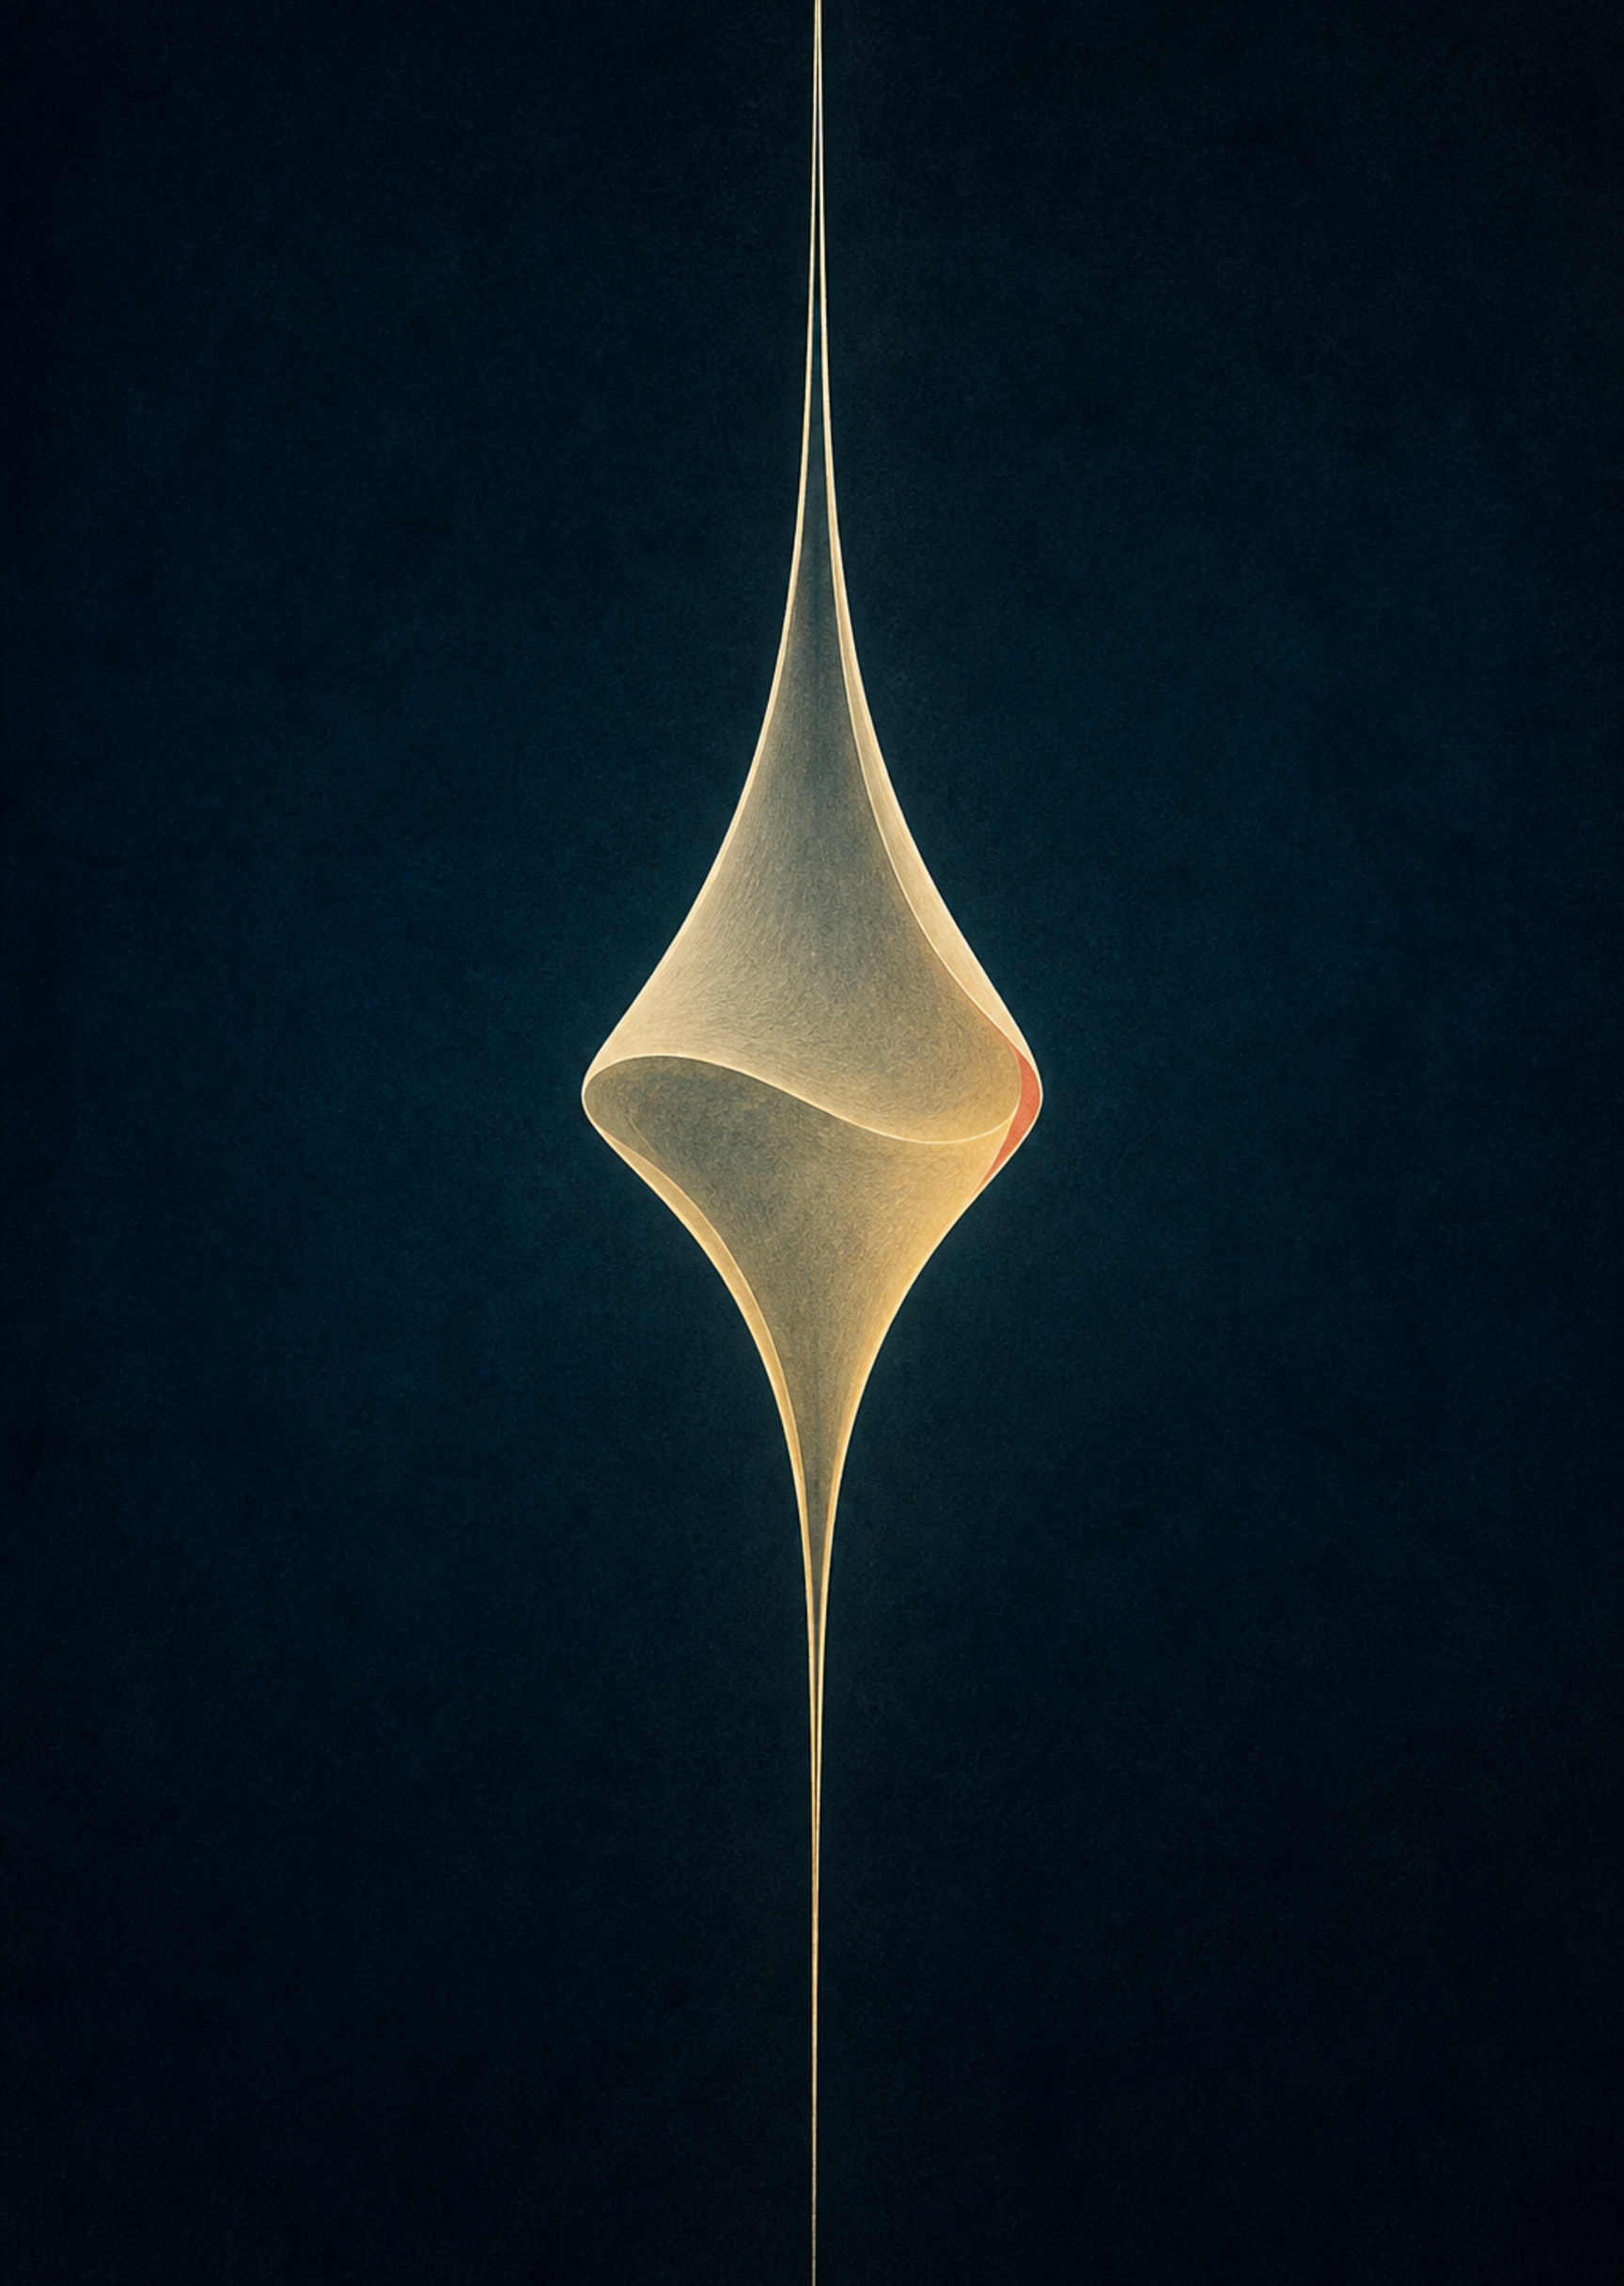
\includegraphics[height=\paperheight,keepaspectratio]{../../../generated_course_notes/supplementary/string_theory/2010_fall_string_theory_and_m_theory/assets/cover-art.png}%
  };
  \node[
    anchor=north west,
    align=left,
    text width=0.78\paperwidth,
    fill=white,
    fill opacity=0.9,
    rounded corners=8pt,
    inner xsep=10pt,
    inner ysep=8pt
  ] at ([xshift=0.08\paperwidth,yshift=-0.06\paperheight]current page.north west) {%
    {\fontsize{30}{33}\selectfont\bfseries\color{black!88} 弦理论与M理论\\[0.85em]}
    {\large\color{black!72} 中文版 / 2010 fall string theory and m theory}
  };
  \node[
    anchor=south west,
    align=left,
    text width=0.68\paperwidth,
    fill=white,
    fill opacity=0.82,
    text opacity=1,
    rounded corners=6pt,
    inner sep=12pt
  ] at ([xshift=0.08\paperwidth,yshift=0.08\paperheight]current page.south west) {%
    {\normalsize\color{black!78} 原讲授：Leonard Susskind\\[0.35em]}
    {\small\color{black!72} 讲义辅助版本：\href{https://lazying.art}{LazyingArt LLC} / \href{https://github.com/lachlanchen/Video2Book}{Video2Book}}
  };
\end{tikzpicture}
\mbox{}
\end{titlepage}
\hypersetup{pageanchor=true}

\clearpage
\chapter*{关于本讲义}
这些经过独立编辑的配套讲义依据 Leonard Susskind 的讲座整理而成。它们由机器转录文本、字幕以及选定的黑板画面重建，并与可获得的原始材料进行了核对。它们并非 Susskind 教授的原稿，也未经其审阅或认可。

本版本由 \href{https://lazying.art}{LazyingArt LLC} 使用开源 \href{https://github.com/lachlanchen/Video2Book}{Video2Book} 工作流程制作。机器转录文本另行提供，可能包含识别错误。编辑性澄清与非平凡的重建均在脚注中标明。
\clearpage
\tableofcontents
\mainmatter
\chapter{从强子Regge轨迹到光锥弦}

\lectureoverview{弦理论最初并不是作为量子引力理论而诞生的。它起初是为了理解强子的谱与散射。笔直的Regge轨迹暗示存在一个延展客体；{\proseunicodefont π}介子--{\proseunicodefont π}介子散射中的对偶性则暗示，两个表面上不同的过程其实是同一曲面的两种切片方式。我们将沿着这些线索进入世界面图像，把强子弦重新解释为QCD流管，然后利用无限动量参照系推导开弦的横向力学。核心结果是，其有效内部哈密顿量度量的是质量的平方。因此，在该描述中与\(L^2\)成正比的胡克定律能量，就变成与\(L\)成正比的静止能量，这正是具有恒定张力的弦的定义性行为。}

\section{弦理论的强子起源}

大约在1968--1970年，导致弦理论出现的问题涉及质子、中子，尤其是介子。夸克模型当时已经是一个严肃的想法，但强子的夸克组分尚未以现代意义在实验上得到确立。胶子在通常讨论中的地位就更不显著了。南部曾提出过相关的规范场思想，但量子色动力学的成熟语言当时还不存在。当时的原材料反而是强相互作用粒子异常丰富的谱。

暂时忽略质子--中子的区分，把两种状态都称为核子，这是有用的。核子之外还有自旋更大的更重状态，接着是自旋更大的更重状态。Chew和Frautschi把这样的族组织在一张图上，纵轴是角动量，横轴是质量的平方。按当时的历史单位，质子质量约为1 BeV；同一单位现在称为GeV。

以\(\hbar\)为单位来度量角动量。对于重子族，无量纲自旋值为半整数，

\begin{equation}
  J=\frac12,\frac32,\frac52,\ldots,
\end{equation}

而介子族具有整数自旋。引人注目的经验事实是，无论哪一族，当以\(M^2\)为横轴作图时，都近似落在一条直线上。用现代记号可写为

\begin{equation}
  J\simeq \alpha_0+\alpha' M^2,
  \label{eq:l01-regge-trajectory}
\end{equation}

其中\(\alpha_0\)是截距，\(\alpha'\)是Regge斜率。\editorialnote{本讲强调所观测到的线性关系及其近乎普适的斜率。引入截距记号只是为了紧凑地陈述该关系；这些轨迹是经验的、近似的。}

最初的直线并不令人信服，因为它只经过两个已知点。任意两点都确定一条直线。令人惊讶的是后来发生的事：新发现的状态继续落在同一条直线附近。介子轨迹也显示出同样的组织方式。{\proseunicodefont π}介子从\(J=0\)附近开始，在GeV尺度上质量很小；{\proseunicodefont ρ}介子从\(J=1\)开始；进一步的激发继续向上延伸。一个族中可能出现五、六或七个状态。更引人注目的是，不同的重子和介子轨迹几乎平行。因此，角动量增加一个量子，对应着质量的平方增加大致相同的量：

\begin{equation}
  \Delta J=1
  \quad\Longrightarrow\quad
  \Delta M^2\simeq \frac{1}{\alpha'}.
  \label{eq:l01-regge-spacing}
\end{equation}

\begin{classroomqa}
\audiencequestion{不同的Regge轨迹平行意味着什么？\lecturetimestamp{00:09:32}}
\lecturerresponse{选取一族粒子，画出它的所有激发态；它们落在一条直线上。对另一个介子族或重子族重复这一做法。即使截距不同，这些直线也具有大致相同的斜率。因此，角动量增加相同的量，所付出的\(M^2\)增量也大致相同。这一共同的斜率被称为普适Regge斜率。}
\end{classroomqa}

与普通延展客体的比较说明了这一模式为何重要。篮球被旋转时会获得转动能量，但它的轨迹是弯曲的而非直线的，而且在角速度足够高时，球会被撕裂。原子也有转动激发，但最终会被电离；它的轨迹会终止。强子则显示出简单得多的序列，而且在现有数据范围内，没有迹象表明该序列会终止。

这一谱表明，强子的行为不像一个点。点没有可供旋转或形变的空间结构。电子没有观测到更高自旋内部态的塔，因而在目前的实验界限内是类点的。相比之下，强子可以被旋转起来。它的谱暗示了复合性，而自旋与质量之间的关系则暗示，该客体随着角动量增加而发生形变。

\section{{\proseunicodefont π}介子--{\proseunicodefont π}介子散射中的对偶性}

光谱学提供了一条线索。{\proseunicodefont π}--{\proseunicodefont π}散射提供了另一条线索。两个{\proseunicodefont π}介子可以结合成一个类{\proseunicodefont ρ}共振态，随后又作为两个{\proseunicodefont π}介子重新出现。在传统的费曼图中，这是一个湮灭与再产生过程，习惯上称为\(s\)道过程。把同一个基本图旋转过来，就得到一个交叉的，即\(t\)道过程，其中{\proseunicodefont π}介子之间交换了一个类{\proseunicodefont ρ}粒子。

{\proseunicodefont ρ}并不孤单。它属于一个Regge族，因此自洽性似乎要求在两个道中都包含{\proseunicodefont ρ}及其所有激发伙伴。示意地，

\begin{equation}
  \mathcal A(s,t)\simeq
  \sum_n \mathcal A^{(s)}_{\rho_n}(s,t),
  \qquad
  \mathcal A(s,t)\simeq
  \sum_n \mathcal A^{(t)}_{\rho_n}(s,t).
  \label{eq:l01-channel-sums}
\end{equation}

这些表达式并不是两个应当简单相加的近似。数值研究发现，在湮灭道中对共振塔求和，已经给出了大致相当于交换道所预期的贡献。反过来，交换的塔也能重现共振描述。因此，把两个完整的塔相加，似乎把同一物理计算了两次。通常的微扰记账法说，如果两个图存在，就必须都包括进来。而强子振幅却暗示，这两种道的描述是对偶的。

\begin{figure}[H]
  \centering
  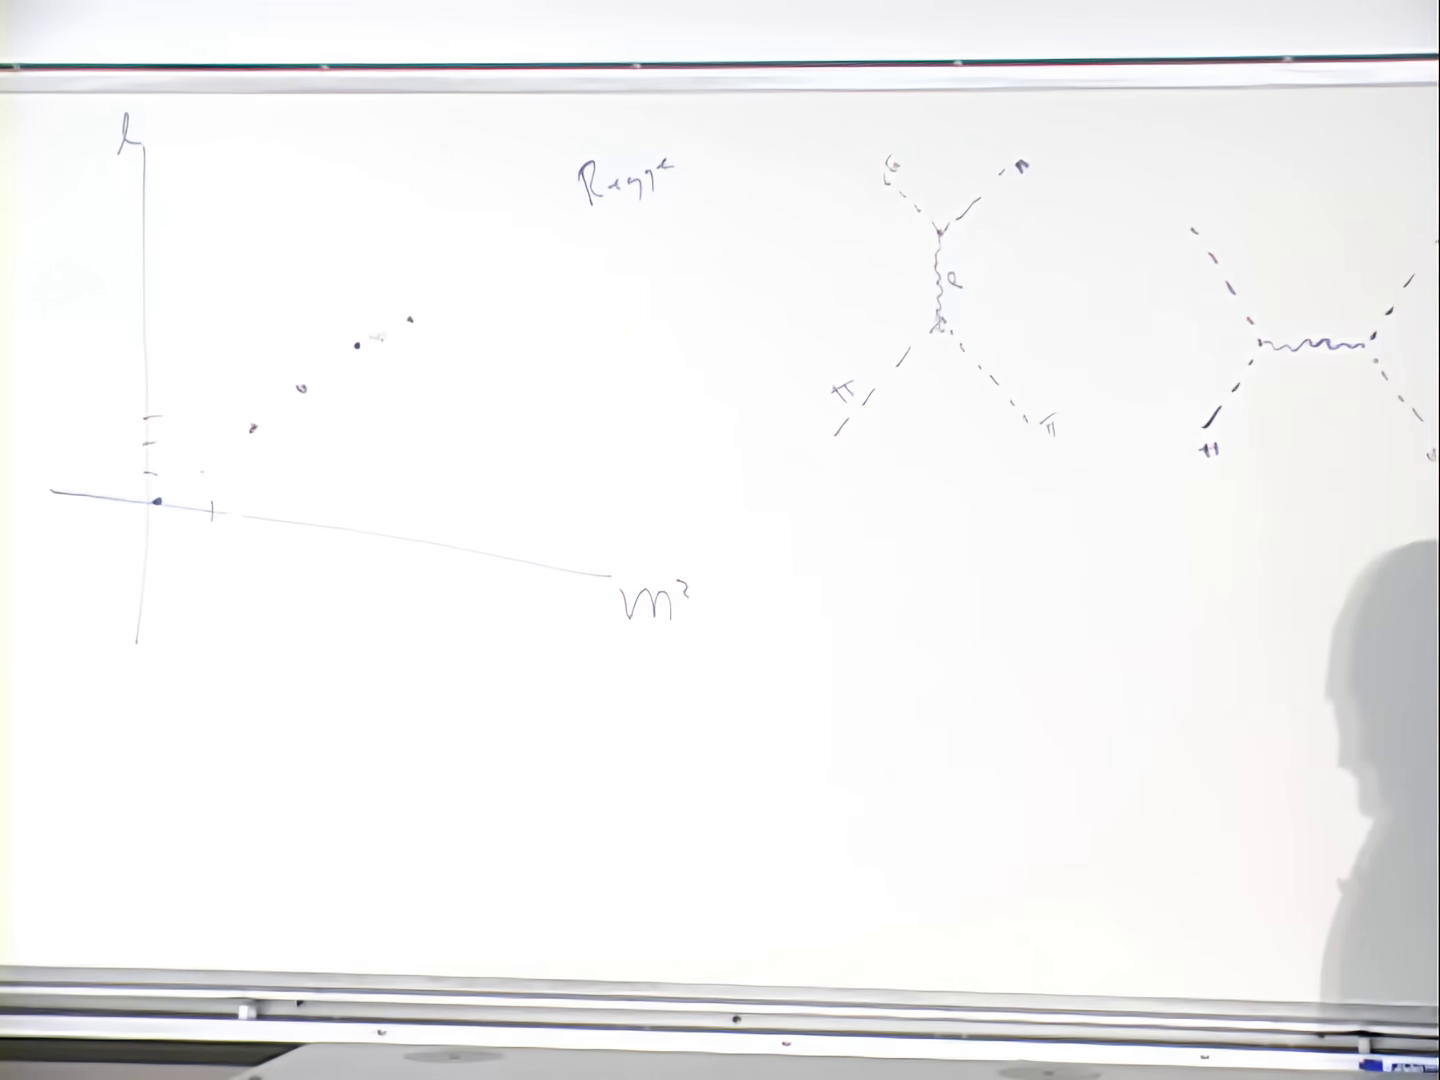
\includegraphics[width=0.82\textwidth]{lecture_01_figure_01.png}
  \caption{这张图把Chew--Frautschi图与湮灭道和交叉道图联系起来，使光谱线索和散射线索成为同一个问题的一部分。}
  \lectureframe{00:14:20}
  \label{fig:l01-regge-duality-board}
\end{figure}

同样的关系可以分离成一个清晰的示意图。第一个面板记录了线性谱；另外两个表示同一振幅的另一种道展开。

\begin{figure}[H]
  \centering
  \resizebox{\textwidth}{!}{%
  \begin{tikzpicture}[>=Latex,thick]
    \begin{scope}
      \draw[->] (0,0) -- (4.2,0) node[right] {$M^2$};
      \draw[->] (0,0) -- (0,3.4) node[above] {$J$};
      \draw[blue!65!black] (0.45,0.35) -- (3.55,2.95);
      \draw[orange!80!black] (0.75,0.20) -- (3.85,2.80);
      \foreach \x/\y in {0.65/0.52,1.35/1.10,2.05/1.69,2.75/2.27,3.45/2.86}
        \fill[blue!65!black] (\x,\y) circle (0.07);
      \foreach \x/\y in {0.95/0.37,1.65/0.95,2.35/1.54,3.05/2.12,3.75/2.71}
        \fill[orange!80!black] (\x,\y) circle (0.07);
      \node at (2.1,-0.55) {parallel Regge families};
    \end{scope}
    \begin{scope}[xshift=5.7cm]
      \draw[->] (-1.5,1.2) -- (-0.3,0.25);
      \draw[->] (-1.5,-1.2) -- (-0.3,-0.25);
      \draw[decorate,decoration={snake,amplitude=1.5pt,segment length=7pt}]
        (0,0.25) -- (0,-0.25);
      \draw[->] (0.3,0.25) -- (1.5,1.2);
      \draw[->] (0.3,-0.25) -- (1.5,-1.2);
      \node at (0,-1.75) {$s$-channel tower};
    \end{scope}
    \begin{scope}[xshift=10.5cm]
      \draw[->] (-1.5,1.2) -- (1.5,1.2);
      \draw[->] (-1.5,-1.2) -- (1.5,-1.2);
      \draw[decorate,decoration={snake,amplitude=1.5pt,segment length=7pt}]
        (0,0.95) -- (0,-0.95);
      \node at (0,-1.75) {$t$-channel tower};
    \end{scope}
  \end{tikzpicture}}
  \caption{平行的Regge族以及强子对偶中涉及的两种道展开。}
  \label{fig:l01-regge-duality-redraw}
\end{figure}

\section{一个世界面，两种切片方式}

自然的回应是寻找一段可以用两种方式解读的几何历史。用夸克--反夸克对表示一个{\proseunicodefont π}介子，并让时间向上流动。不要只画一维的粒子线，而是填充由夸克轨迹围成的区域。对这一二维历史作水平切片，可能显示两条入射弦结合，随后又分开。换一种切片方式，则显示一条弦从一侧交换到另一侧。这两幅费曼道图像不再是彼此独立的机制；它们是同一个曲面的不同分解。

\begin{figure}[H]
  \centering
  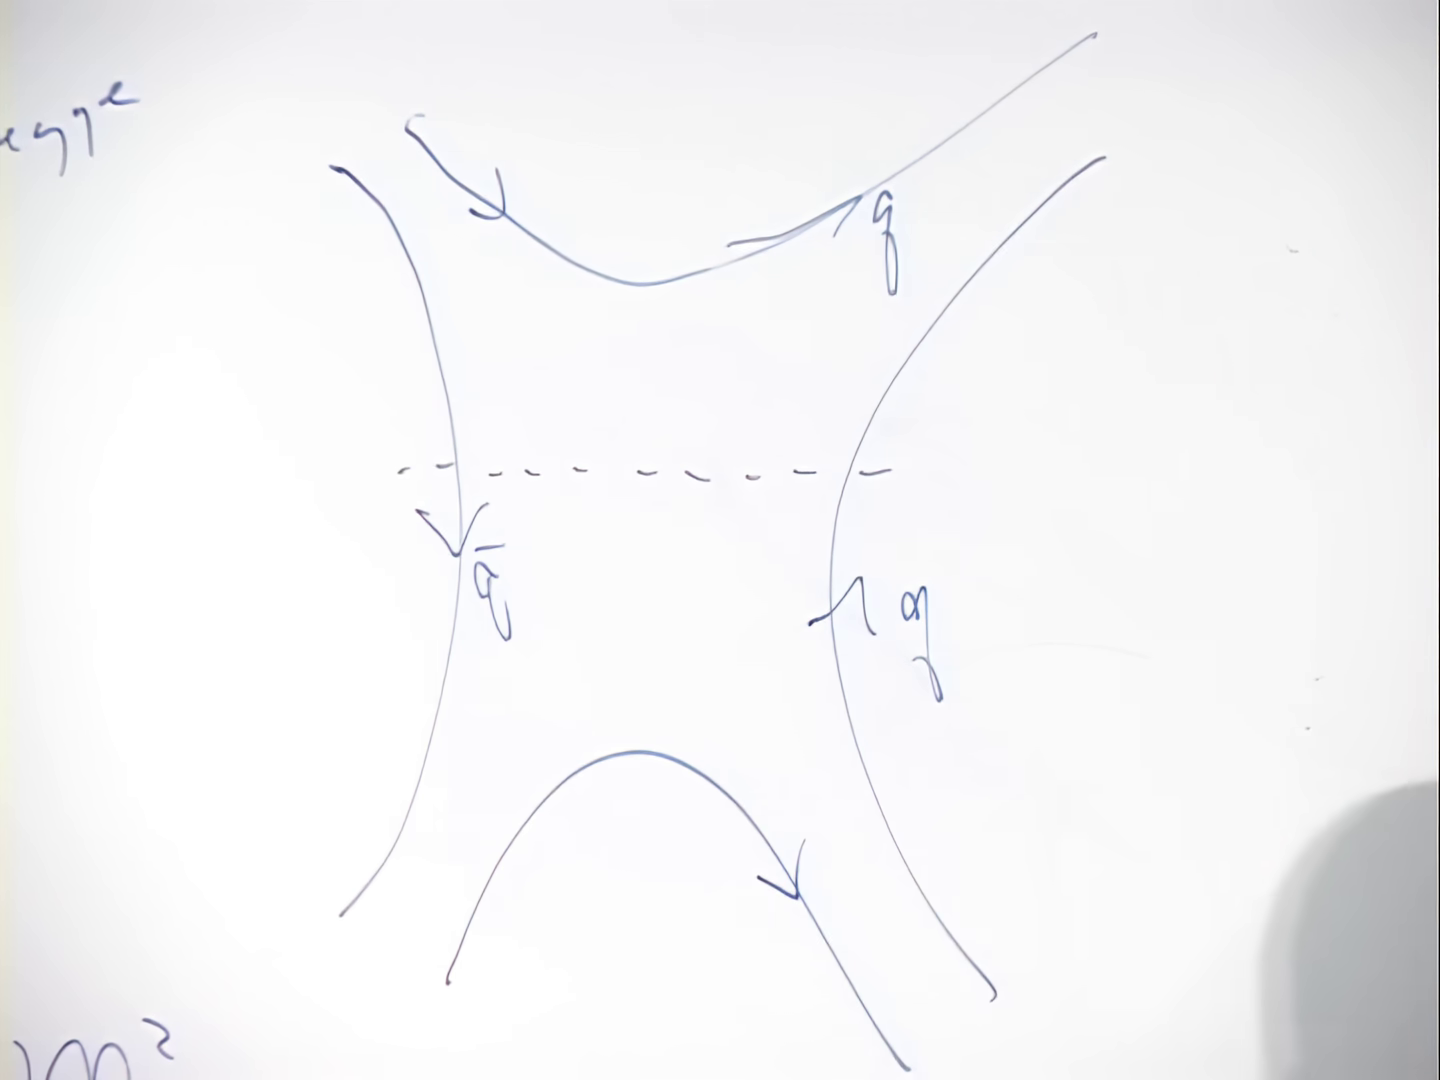
\includegraphics[width=0.78\textwidth]{lecture_01_figure_02.png}
  \caption{图上的夸克线拓扑。对同一二维历史作不同的切割，产生共振解读和交换解读。}
  \lectureframe{00:17:50}
  \label{fig:l01-worldsheet-topology-board}
\end{figure}

夸克与反夸克之间的区域提供了进一步的想法。在固定时刻，切片包含两个端点以及填满它们之间整个区间的某种东西。那个东西是一维的：一条弦。在相互作用过程中，弦扫出一个二维曲面。

\begin{definition}
点粒子的时空历史是一条\emph{世界线}。弦的时空历史是一个\emph{世界面}。某一瞬间的弦是其世界面的一个空间切片。
\end{definition}

\begin{figure}[H]
  \centering
  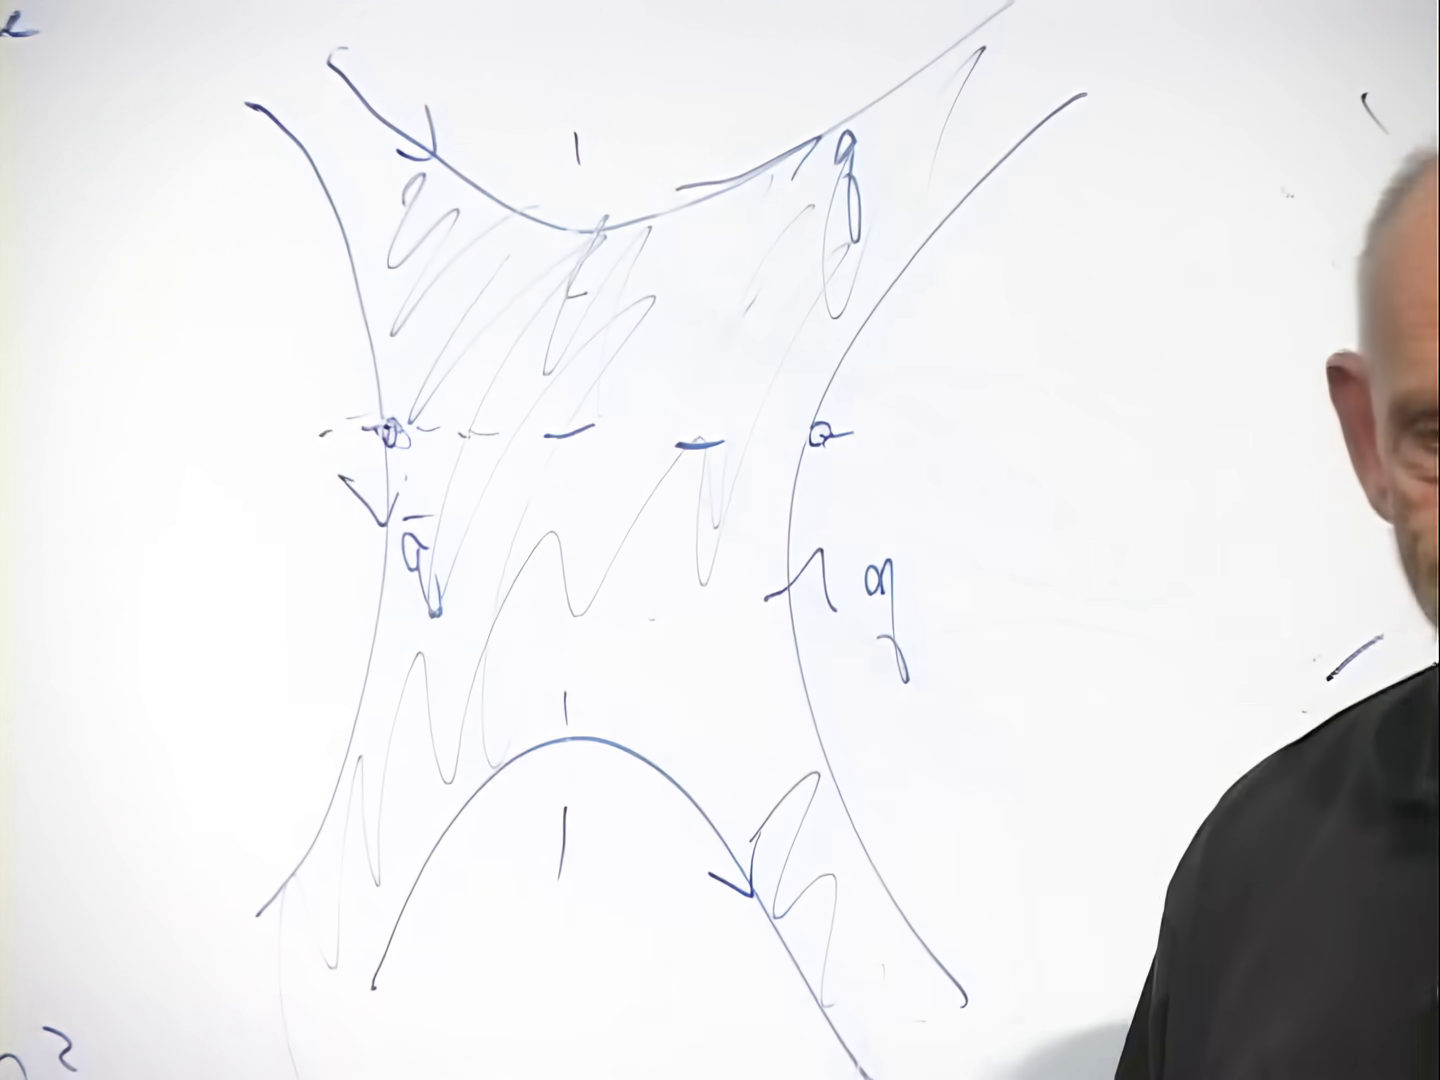
\includegraphics[width=0.78\textwidth]{lecture_01_figure_03.png}
  \caption{图上填充在端点轨迹之间的曲面。一个时间切片与它相交，得到一条一维弦。}
  \lectureframe{00:19:15}
  \label{fig:l01-worldsheet-filled-board}
\end{figure}

\begin{figure}[H]
  \centering
  \begin{tikzpicture}[>=Latex,scale=0.95]
    \fill[blue!10]
      (-2.6,-2.3) .. controls (-1.0,-1.0) and (-1.0,-0.4) .. (-0.2,0)
      .. controls (-1.0,0.5) and (-1.0,1.0) .. (-2.6,2.3)
      -- (2.6,2.3)
      .. controls (1.0,1.0) and (1.0,0.5) .. (0.2,0)
      .. controls (1.0,-0.4) and (1.0,-1.0) .. (2.6,-2.3) -- cycle;
    \draw[blue!65!black]
      (-2.6,-2.3) .. controls (-1.0,-1.0) and (-1.0,-0.4) .. (-0.2,0)
      .. controls (-1.0,0.5) and (-1.0,1.0) .. (-2.6,2.3);
    \draw[blue!65!black]
      (2.6,-2.3) .. controls (1.0,-1.0) and (1.0,-0.4) .. (0.2,0)
      .. controls (1.0,0.5) and (1.0,1.0) .. (2.6,2.3);
    \draw[red!75!black,dashed] (-2.9,-1.15) -- (2.9,-1.15)
      node[right] {time slice};
    \draw[orange!80!black,dashed] (-1.55,-2.5) -- (1.55,2.5)
      node[above] {crossed slicing};
    \draw[->] (3.45,-1.7) -- (3.45,1.8) node[above] {time};
    \node[blue!65!black] at (0,-2.7) {one world sheet};
  \end{tikzpicture}
  \caption{一个清晰的世界面示意图。不同的切片方式把同一个曲面组织成不同的中间道描述。}
  \label{fig:l01-worldsheet-redraw}
\end{figure}

这种几何重构是探索性的，并不是从第一性原理推导出完整理论。不同的人以不同方式达到了早期的弦图像。它的力量在于，同一个延展物体可以同时处理这两种观测：弦可以旋转和形变，而它的世界面可以编码对偶的散射道。

\begin{classroomqa}
\audiencequestion{为什么要引入一个弦状的桥梁，而不是在夸克之间交换一个普通粒子？\lecturetimestamp{00:21:20}}
\lecturerresponse{在某一瞬间，不仅仅存在一个局域化的交换粒子。存在一个夸克、一个反夸克，以及它们之间所有点处的结构。这种结构可能是基本连续的，也可能是大量组分密集聚集而近似为连续体；第一种图像并未作出判定。重要的是整个区间都被占据，而且观测到的轨迹没有表现出像两端系着重物的普通鞋带那样终止的倾向。}
\end{classroomqa}

\begin{classroomqa}
\audiencequestion{标准模型能描述{\proseunicodefont π}介子散射吗？
\lecturetimestamp{00:22:45}}
\lecturerresponse{能，尽管其有用性取决于能区。在低能下，标准模型通过QCD及其低能描述，能够解释大量的{\proseunicodefont π}介子散射。在较高能量下，当整族的强子交换都变得重要时，直接计算变得更加困难，而弦式的组织方式可能更为有用。}
\end{classroomqa}

\begin{classroomqa}
\audiencequestion{早期实验是否确立了Regge轨迹永不终止？\lecturetimestamp{00:23:37}}
\lecturerresponse{没有。它们只确立了所观测到的序列尚未显示出终点。关于可无限延伸的推断是一种富有启发性的外推，而不是被测量到的无限。}
\end{classroomqa}

\section{通量管与标度的变化}

现代QCD为这一旧图像提供了场论解释。夸克与反夸克充当胶子场的相反源。在普通电动力学中，当相反电荷被分开时，电通量会向侧面扩展。场随距离减弱，因此电荷之间的区域不会保持固定的横向剖面。QCD是非线性的。其动力学可以将相关的色电场通量限制在连接夸克与反夸克的狭窄管中。

\begin{figure}[H]
  \centering
  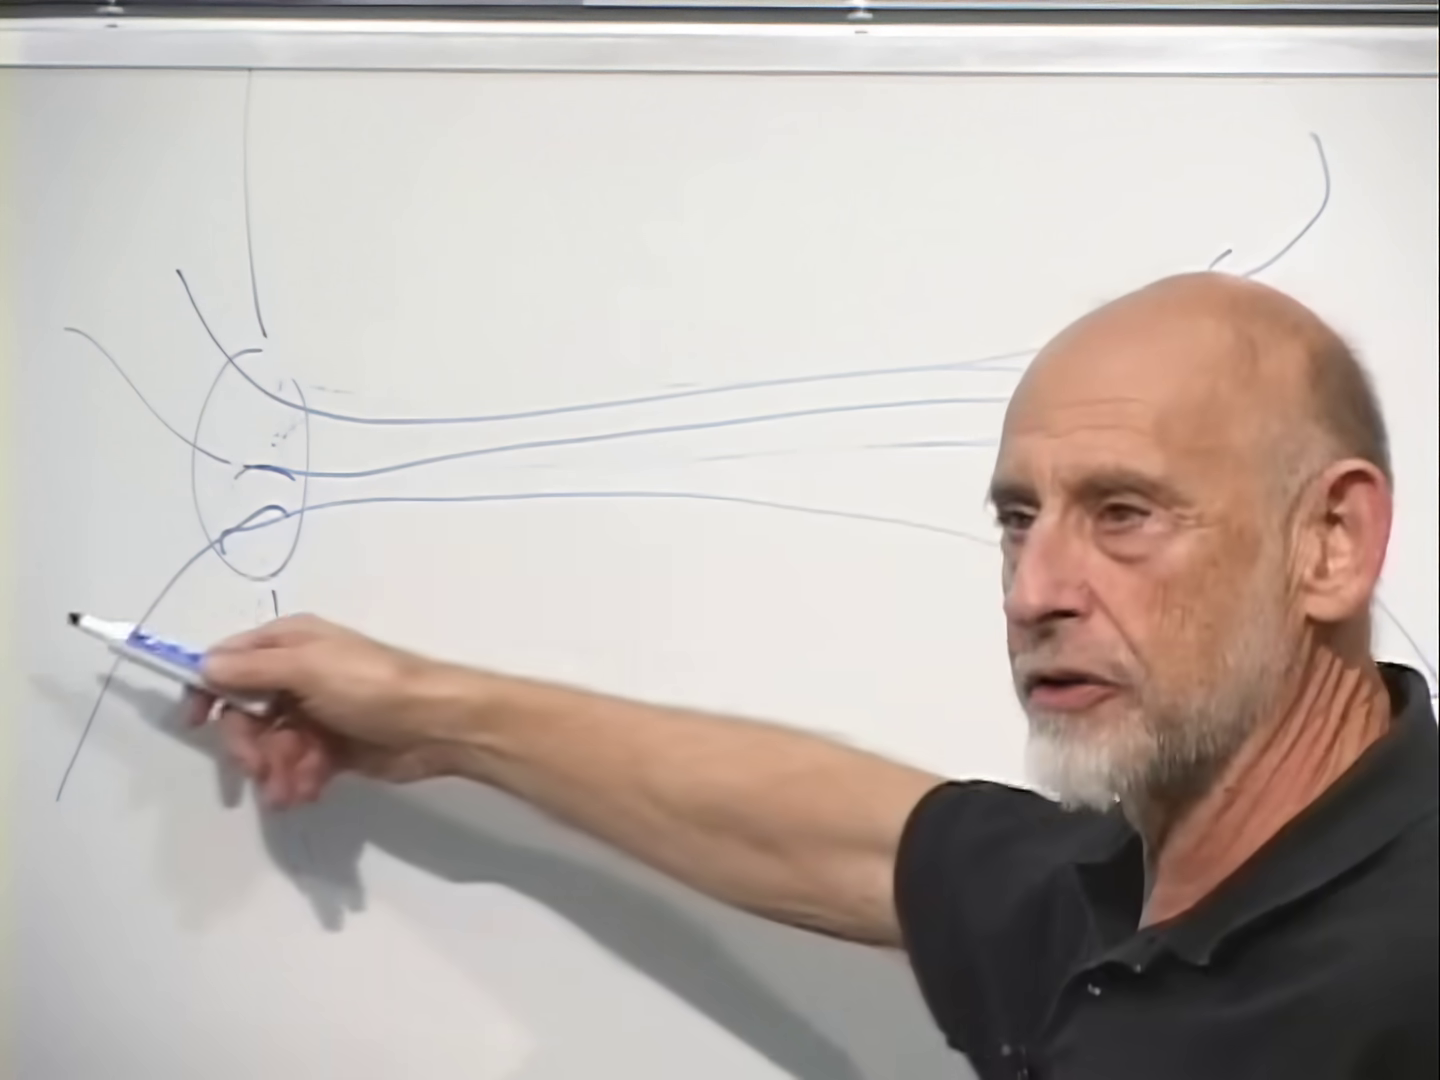
\includegraphics[width=0.78\textwidth]{lecture_01_figure_04.png}
  \caption{夸克与反夸克的场线被画成狭窄的通量管，而不是自由扩展的库仑场。}
  \lectureframe{00:25:15}
  \label{fig:l01-qcd-flux-board}
\end{figure}

\begin{figure}[H]
  \centering
  \begin{tikzpicture}[>=Latex]
    \fill[orange!14,rounded corners=8pt] (-3.0,-0.55) rectangle (3.0,0.55);
    \draw[orange!80!black,thick,rounded corners=8pt]
      (-3.0,-0.55) rectangle (3.0,0.55);
    \fill[blue!70!black] (-3.35,0) circle (0.17);
    \fill[red!75!black] (3.35,0) circle (0.17);
    \node[below] at (-3.35,-0.22) {$q$};
    \node[below] at (3.35,-0.22) {$\bar q$};
    \foreach \y in {-0.30,0,0.30}
      \draw[->,orange!85!black] (-3.05,\y) -- (3.05,\y);
    \draw[<->] (-2.9,-1.05) -- (2.9,-1.05) node[midway,below] {$L$};
    \node at (0,0.92) {approximately fixed transverse profile};
  \end{tikzpicture}
  \caption{被禁闭的通量管在伸长时不扩展。固定的单位长度能量给出\(E=TL\)。}
  \label{fig:l01-qcd-flux-redraw}
\end{figure}

粒子语言与场语言以不同方式表达同一件事。在场描述中，当两端分离时，管保持大致相同的场强和横截面积。在组分图像中，拉伸能量在两端之间产生更多的胶子结构。普通橡皮筋具有固定数目的分子，因此其分子会彼此分离，直到材料断裂。不妨设想，每当出现一个空隙时就插入一个新分子。这样，沿带的密度可以保持固定，而带却变得更长。这就是对胶子场的预期类比：管获得长度，而不是变细直至断裂。

\begin{classroomqa}
\audiencequestion{构成电子的弦是否也会由胶子组成？\lecturetimestamp{00:28:08}}
\lecturerresponse{得不出这样的结论。强子弦是质子尺度上的QCD客体。与量子引力相关的假想基本弦将位于小得多的普朗克尺度附近，而这里没有证据表明电子是强子胶子弦。引人注目的事实是，相关的数学在两个尺度上都出现了，而不是物理客体本身相同。}
\end{classroomqa}

将强子图像转变为完整的相互作用弦理论的尝试很有前景，但并未完全产生所期望的强子理论。该数学模型一再包含一个自旋为二的无质量粒子。在强子理论中，该态看起来像是一个不受欢迎的预言；而作为引力理论，它具有的量子数恰好就是引力子的量子数。Joel Scherk和John Schwarz作出了决定性的重新解释：也许这个理论告诉我们的不是强子，而是量子引力。强子应用与基本应用在物理上是不同的，尽管早期的强子问题提供了通向这一数学的路径。

\begin{classroomqa}
\audiencequestion{通量线如何从正端点走向负端点？\lecturetimestamp{00:31:46}}
\lecturerresponse{它们离开一个源并进入另一个源，正如磁力线从条形磁铁的北极延伸到南极。相反的端点标记表达了通量的取向；条形磁铁同样具有两个相反的磁极，而不是两个北极。}
\end{classroomqa}

\begin{classroomqa}
\audiencequestion{弦是连续的还是离散的？
\lecturetimestamp{00:32:45}}
\lecturerresponse{量子理论使这一区分变得微妙。电磁场被表示为连续场，同时也具有离散的量子。同样，弦可以被连续地处理，而其激发是量子化的。两种描述都可以是有效的，取决于所提出的问题。}
\end{classroomqa}

\begin{classroomqa}
\audiencequestion{如果穿过世界面的时空切片的角度发生改变，其交线仍然是一条弦吗？\lecturetimestamp{00:34:20}}
\lecturerresponse{是的。改变同时性切片是一种洛伦兹变换。新的切片与该曲面相交所得的弦，处于不同的运动状态。即使一条弦的质心处于静止，其内部也并非静止不动；它可能在振动。``静止''仅指其质心而言。}
\end{classroomqa}

\section{相对论能量的两种展开}

对延展的振动客体作直接的相对论描述颇为不便。有用的策略是找到一个参考系，使其相关运动具有普通非相对论力学的形式。先从单个粒子开始。非相对论情形下可写为

\begin{equation}
  E_{\mathrm{nr}}=\frac{\bm p^2}{2m}+B,
  \label{eq:l01-nonrel-energy}
\end{equation}

其中\(B\)是与总动量无关的内能或束缚能。对于多个无相互作用的粒子，动能项与内能常数项分别相加。由于只有能量差决定运动，与状态无关的相加常数往往可以略去。

精确的相对论能量为

\begin{equation}
  E=\sqrt{\bm p^2c^2+m^2c^4}.
  \label{eq:l01-rel-energy-c}
\end{equation}

\begin{figure}[H]
  \centering
  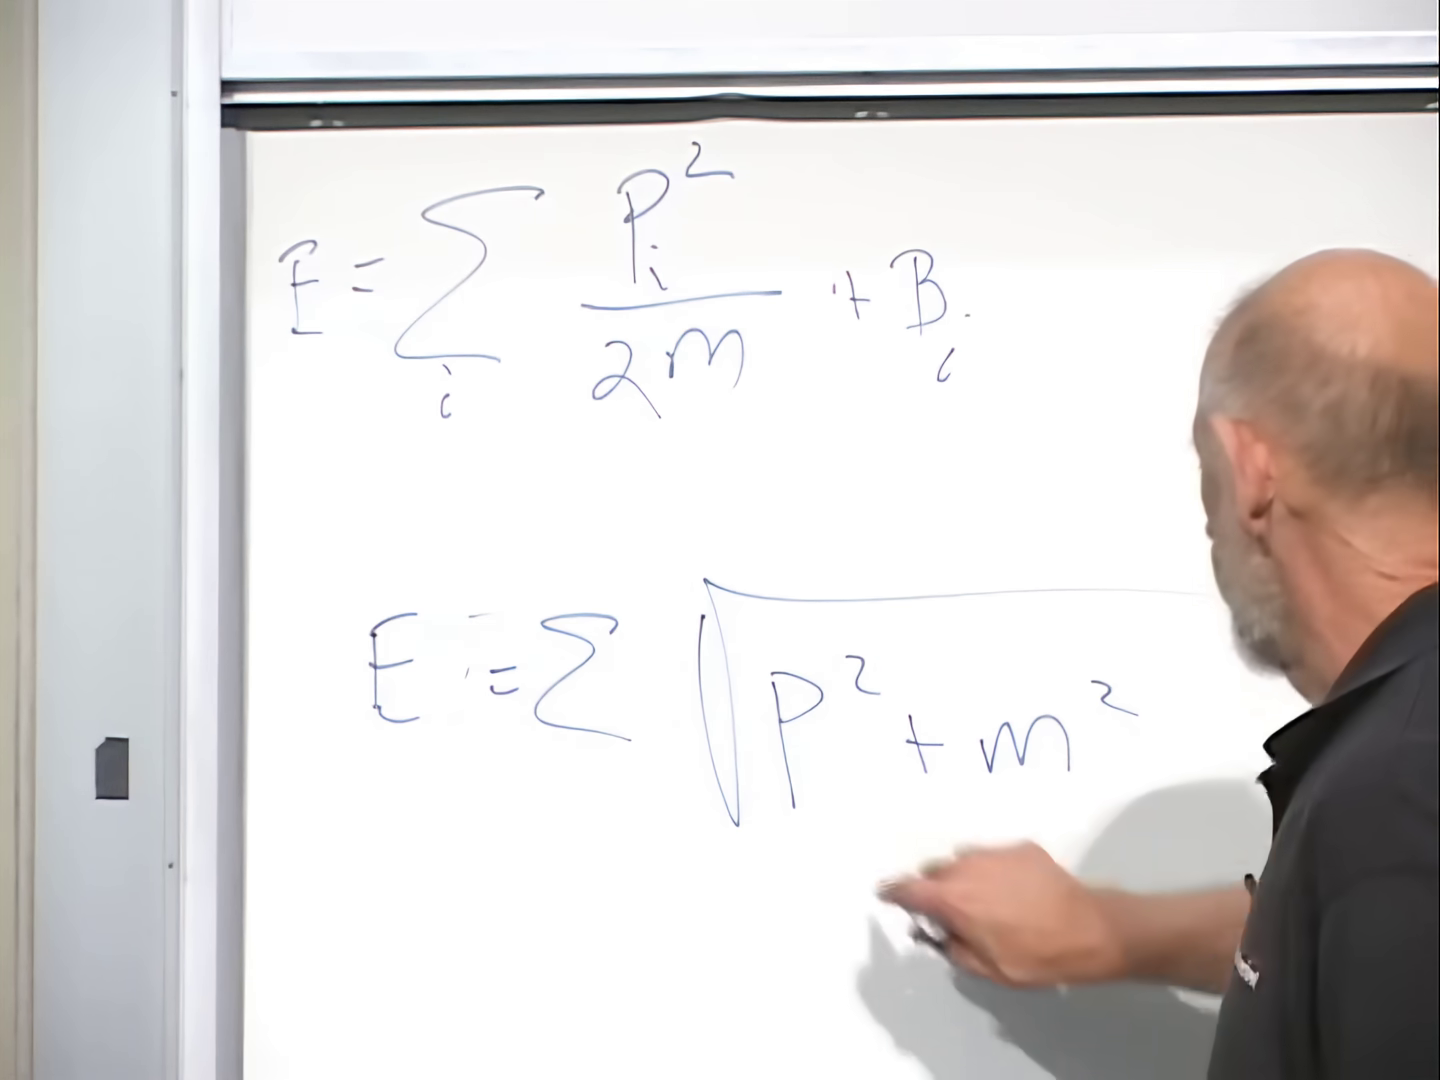
\includegraphics[width=0.76\textwidth]{lecture_01_figure_05.png}
  \caption{非相对论动能与精确的相对论平方根，讨论中已修正\(c\)的幂次。}
  \lectureframe{00:38:45}
  \label{fig:l01-relativistic-energy-board}
\end{figure}

\begin{classroomqa}
\audiencequestion{相对论公式中是否应包含\(p^2c^2\)和
\(m^2c^4\)，而不是最初写在黑板上的那些幂次？
\lecturetimestamp{00:39:12}}
\lecturerresponse{是的。量纲一致性将表达式确定为
\(E^2=p^2c^2+m^2c^4\)。在恢复非相对论极限之后，我们将取
\(c=1\)，但在此处保留这些幂次可使展开更为清晰。}
\end{classroomqa}

当\(p^2c^2\ll m^2c^4\)时，提出\(m^2c^4\)并利用
\(\sqrt{1+\epsilon}\simeq1+\epsilon/2\)：

\begin{align}
  E
  &=mc^2\sqrt{1+\frac{p^2}{m^2c^2}}
  \notag\\
  &\simeq mc^2+\frac{p^2}{2m}.
  \label{eq:l01-low-momentum-expansion}
\end{align}

\begin{figure}[H]
  \centering
  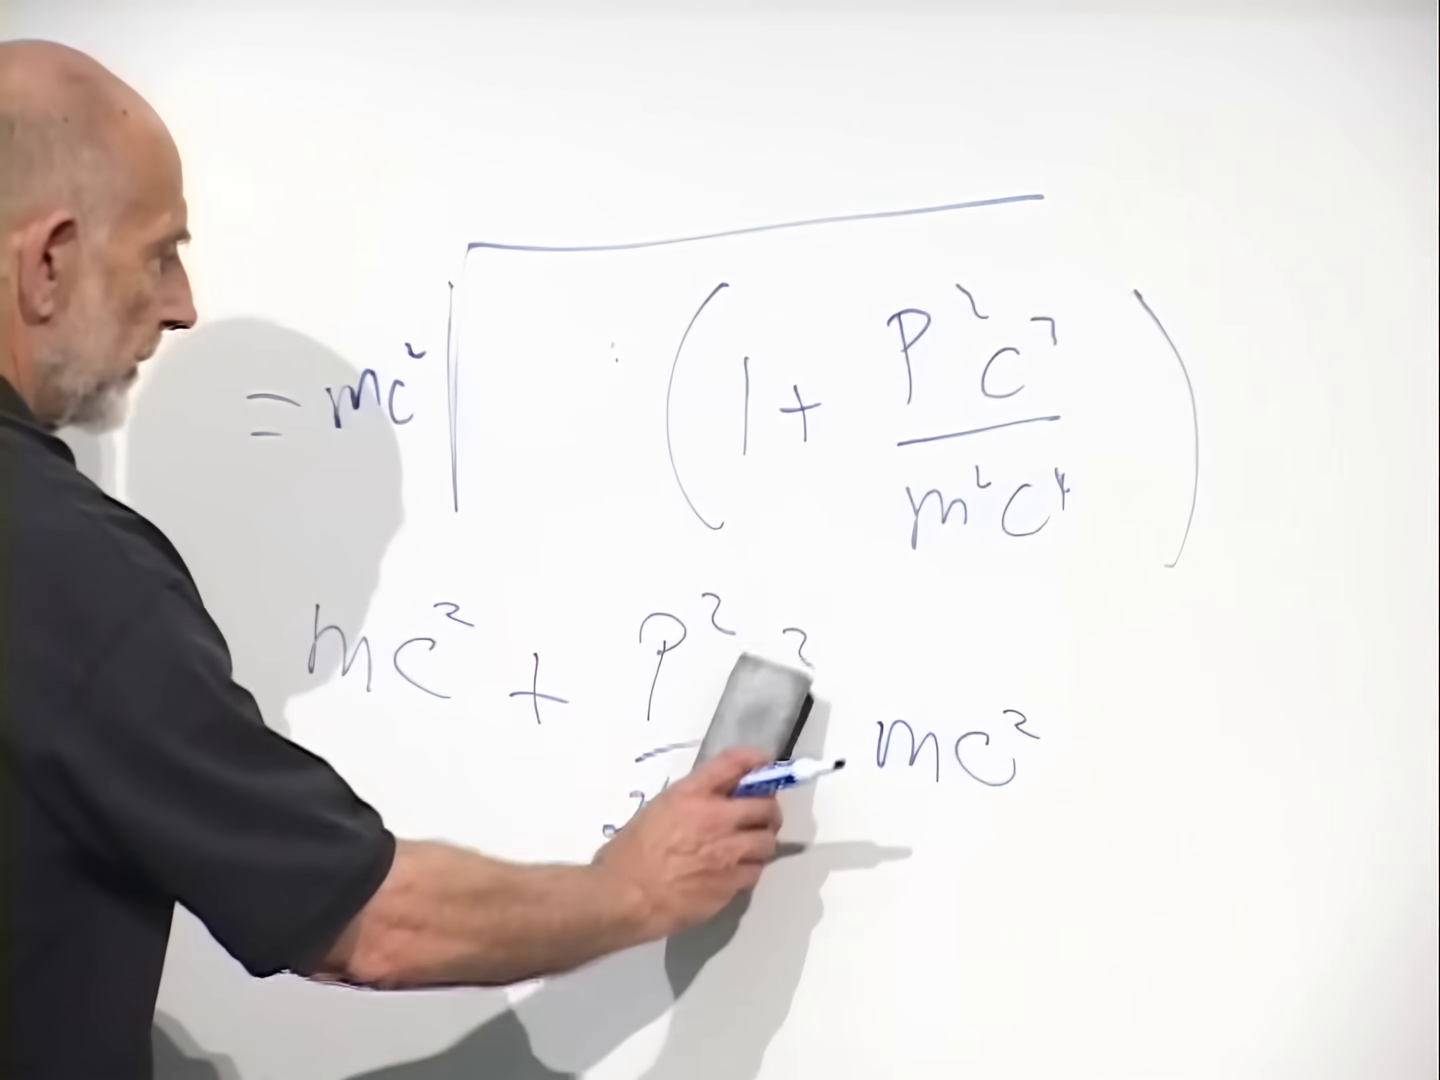
\includegraphics[width=0.76\textwidth]{lecture_01_figure_06.png}
  \caption{小动量展开，恢复出静止能量加上熟悉的非相对论动能项。}
  \lectureframe{00:41:30}
  \label{fig:l01-low-momentum-board}
\end{figure}

这一近似所要求的不仅仅是质心的缓慢运动。一个盒子可以缓慢漂移，而其中的粒子却以接近光速运动。在这种情况下，内部动力学仍然是相对论的。普通的非相对论极限要求所有相关组成粒子的速度在所选参考系中都很小。

还有另一种有用的极限。将整个系统沿\(z\)轴加速，直到每个组成粒子都具有很大的正纵向动量\(P_{zi}\)。任何最初向后运动的组成粒子都会被足够大的加速带到前方。横向动量和静止质量保持不变：

\begin{equation}
  P_{zi}\gg |p_{xi}|,|p_{yi}|,m_i,
  \qquad
  p_{\perp i}^2=p_{xi}^2+p_{yi}^2,
\end{equation}

其中从此刻起\(c=1\)。对大的\(P_{zi}\)作展开得到

\begin{align}
  E_i
  &=\sqrt{P_{zi}^2+p_{\perp i}^2+m_i^2}
  \notag\\
  &=P_{zi}\sqrt{1+\frac{p_{\perp i}^2+m_i^2}{P_{zi}^2}}
  \notag\\
  &\simeq P_{zi}
  +\frac{p_{\perp i}^2+m_i^2}{2P_{zi}}.
  \label{eq:l01-large-pz-one-particle}
\end{align}

\begin{figure}[H]
  \centering
  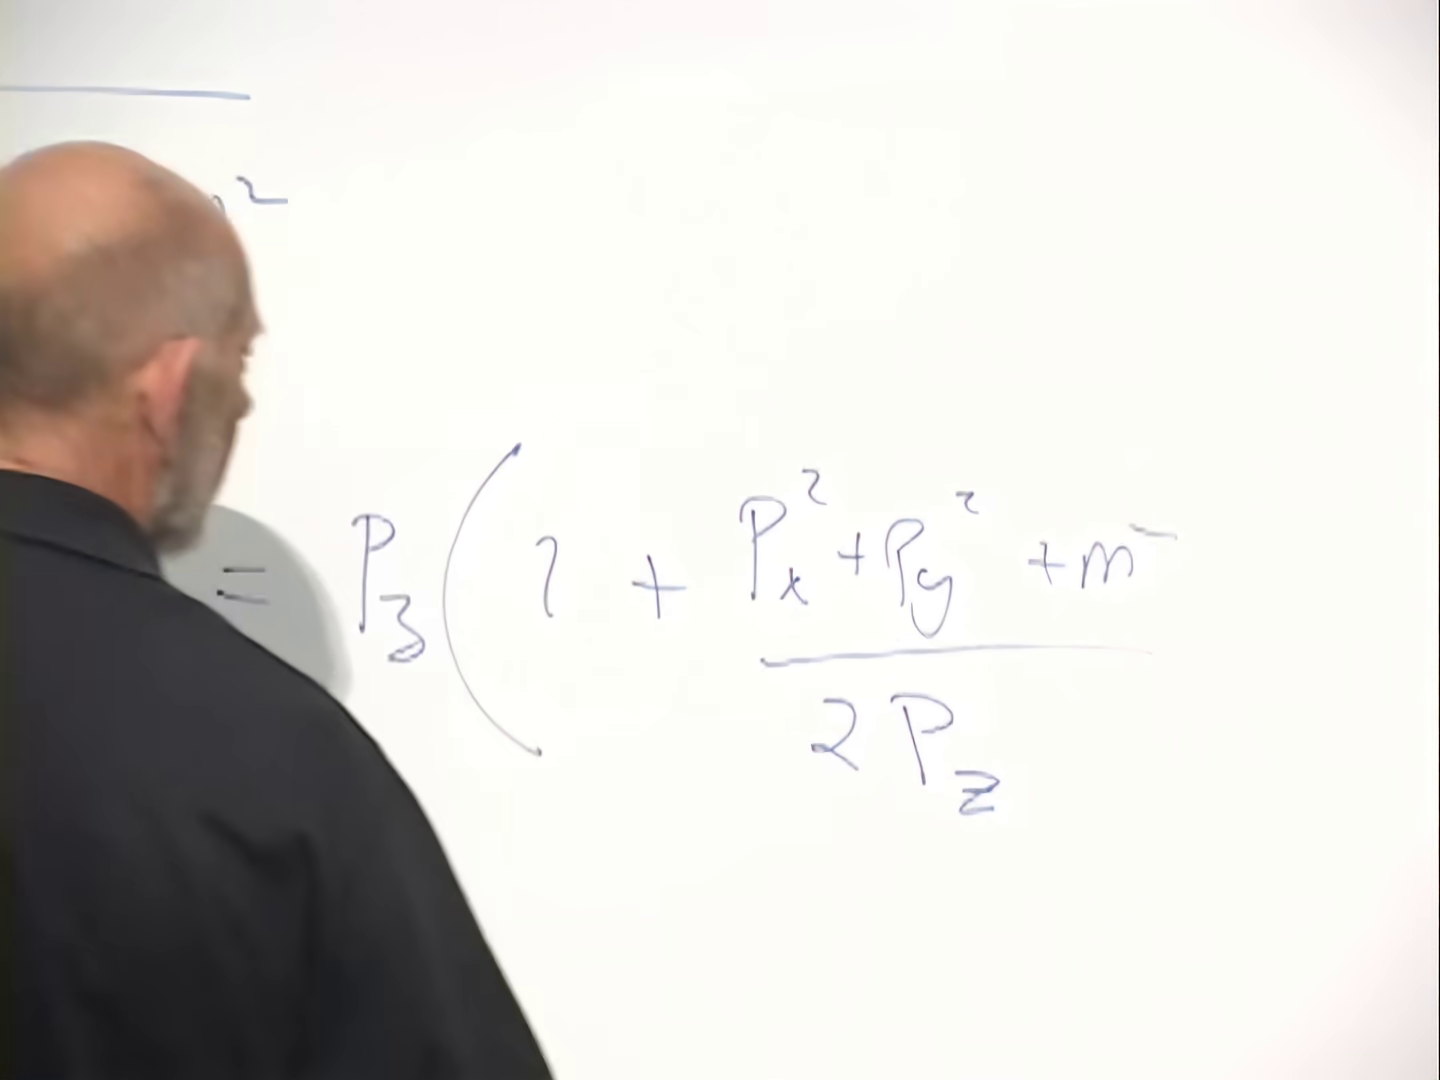
\includegraphics[width=0.76\textwidth]{lecture_01_figure_07.png}
  \caption{大\(P_z\)下的平方根展开，横向动量和质量作为小量保留。}
  \lectureframe{00:46:45}
  \label{fig:l01-large-pz-board}
\end{figure}

对于多个组成粒子，

\begin{equation}
  E\simeq
  \sum_i P_{zi}
  +\sum_i\frac{p_{\perp i}^2}{2P_{zi}}
  +\sum_i\frac{m_i^2}{2P_{zi}}.
  \label{eq:l01-large-pz-sum}
\end{equation}

第一项是守恒的总纵向动量。它极其巨大，但也是一个固定的相加贡献。保留它或减去它都不会改变任何能量差，正如在哈密顿量中加上任何其他守恒量都不会改变运动方程一样。因此动力学部分为

\begin{equation}
  \begin{aligned}
    H_{\perp}=E-P_z
    &\simeq
    \sum_i\left(
      \frac{p_{\perp i}^2}{2P_{zi}}
      +\frac{m_i^2}{2P_{zi}}
    \right),\\
    P_z&=\sum_iP_{zi}.
  \end{aligned}
  \label{eq:l01-transverse-hamiltonian}
\end{equation}

\begin{figure}[H]
  \centering
  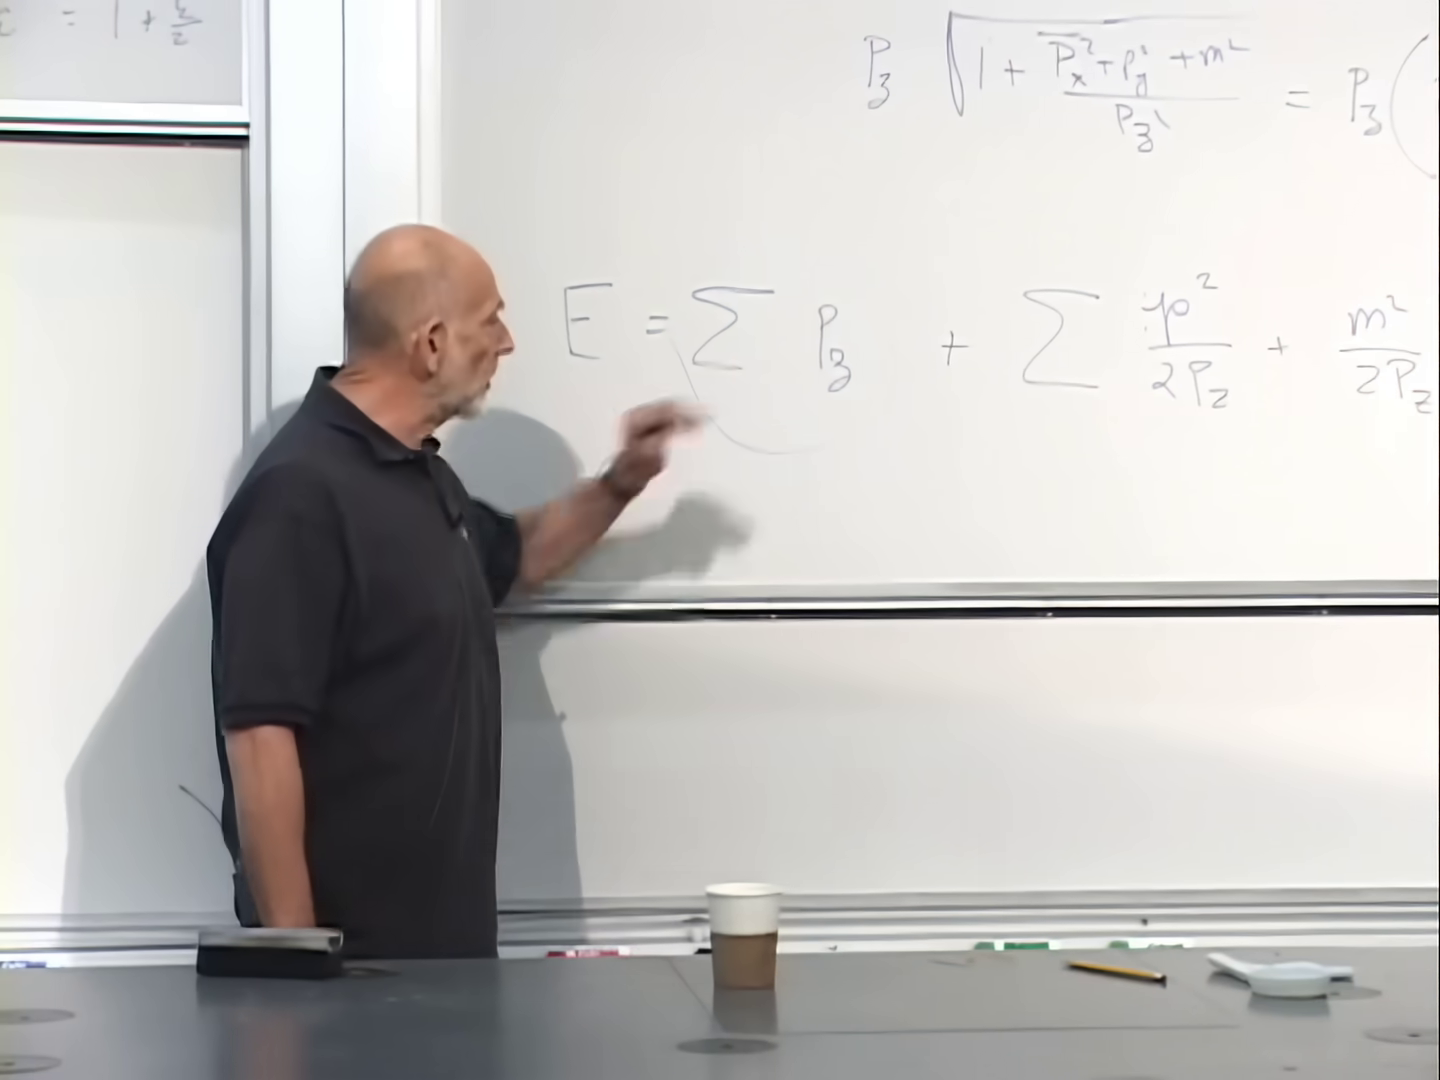
\includegraphics[width=0.78\textwidth]{lecture_01_figure_08.png}
  \caption{多粒子分解为守恒的纵向动量、横向动能以及依赖于质量的内部项。}
  \lectureframe{00:49:16}
  \label{fig:l01-energy-sum-board}
\end{figure}

\section{无限动量参考系}

上述极限在历史上被称为无限动量参考系，现在通常用光锥坐标来表述。其含义可以直接从哈密顿量读出。在量子力学中，

\begin{equation}
  i\hbar\frac{\partial}{\partial t}\ket{\psi}=H\ket{\psi}.
  \label{eq:l01-time-evolution}
\end{equation}

\(H_{\perp}\)中所有非平凡项都按\(1/P_z\)标度。随着加速增大，能量分裂缩小，变化发生得更慢。这就是时间膨胀。一个放射性系统在被高度加速时似乎衰变得更慢；人们可以通过按比例延长观测时间来补偿。这种减慢并未消除动力学。它只是重新标度了它们的时钟。

\begin{figure}[H]
  \centering
  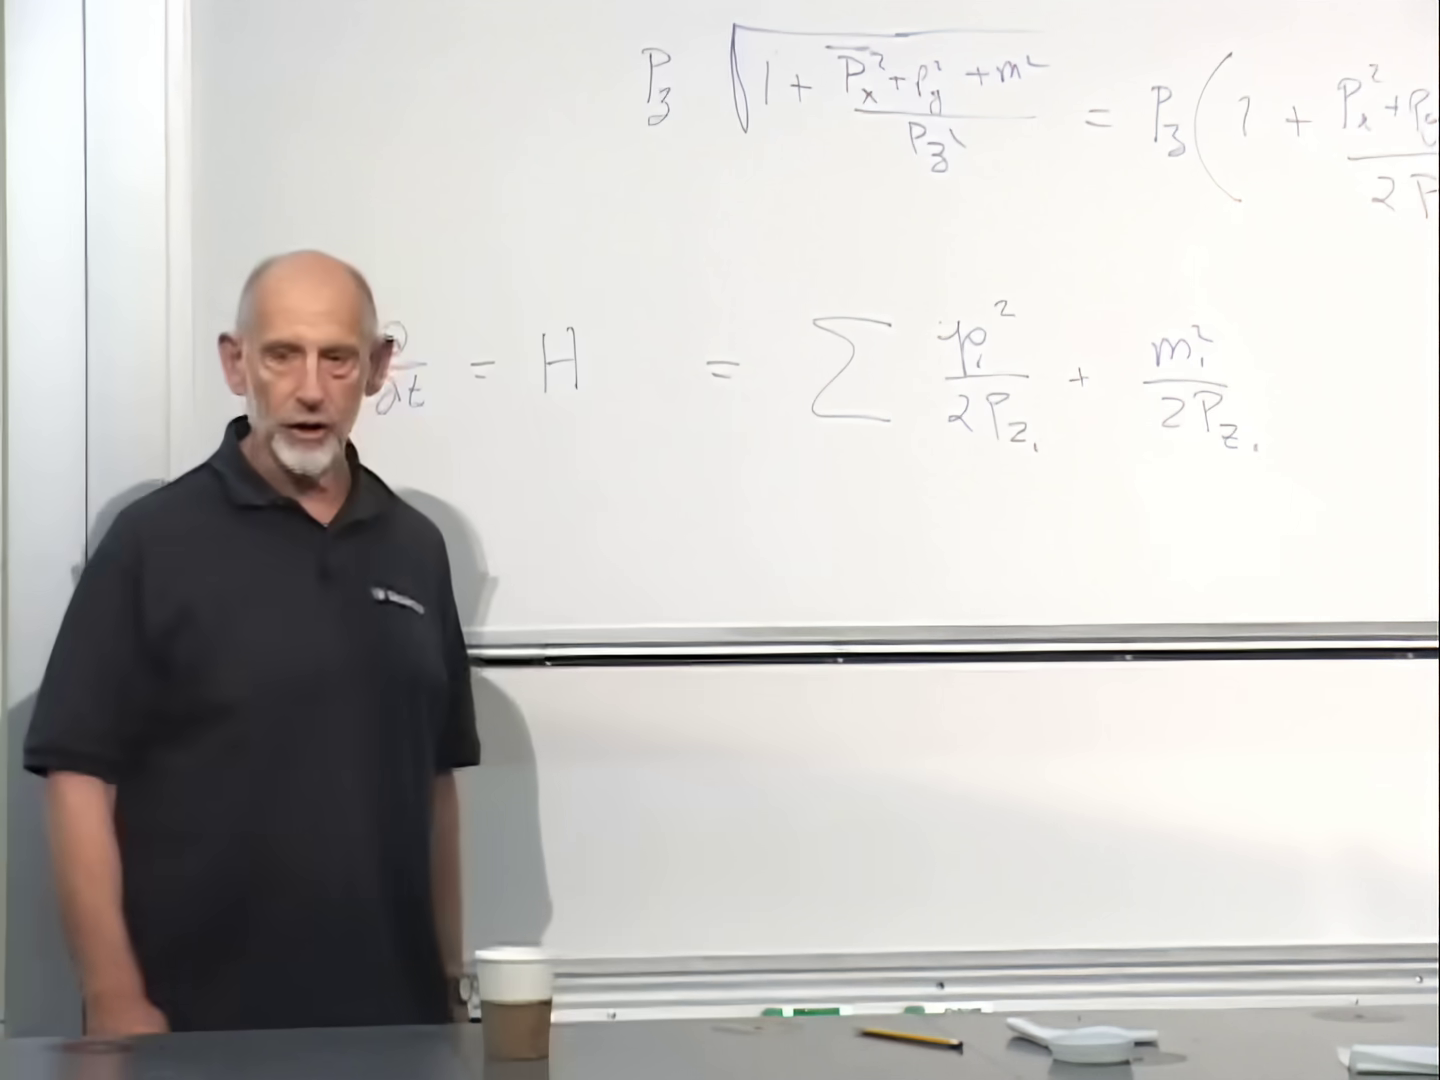
\includegraphics[width=0.78\textwidth]{lecture_01_figure_09.png}
  \caption{黑板上将约化能量等同于产生被加速系统减慢的时间演化的哈密顿量。}
  \lectureframe{00:52:57}
  \label{fig:l01-hamiltonian-board}
\end{figure}

横向项具有精确的非相对论形式 \(p^2/(2m)\)，但质量的角色由 \(P_z\) 扮演。这在物理上是合理的：更大的纵向动量使粒子更难被横向偏转，因此它起到横向惯性的作用。\(m_i^2/(2P_{zi})\) 项不依赖于二维运动状态，因此扮演内能或束缚能的角色。三个空间维度中的相对论运动已变成垂直于推进方向的两个维度中看似非相对论的运动。

这正是使用相对论弦的基本质量-弹簧模型所需的许可。该模型并非假装弦在其静止系中运动缓慢。它使用的是横向动力学具有所需非相对论结构的参考系。

\section{由珠子和弹簧构成的开弦}

取一根开弦，即具有两个端点的弦。之后可能有东西附着在这些端点上，但当前关注的是弦本身。用位于横向位置 \(\bm X_i(t)=(X_i(t),Y_i(t))\) 的珠子来近似它，珠子之间由相同的弹簧连接。离散哈密顿量为

\begin{equation}
  H_N=\sum_{i=1}^{N}
  \left[
    \frac{\mu_N}{2}\dot{\bm X}_i^{\,2}
    +\frac{k_N}{2}
      \left(\bm X_{i+1}-\bm X_i\right)^2
  \right].
  \label{eq:l01-discrete-string}
\end{equation}

仅动能项会使珠子飞散开来。最近邻胡克项才使它们成为一根弦。

\begin{figure}[H]
  \centering
  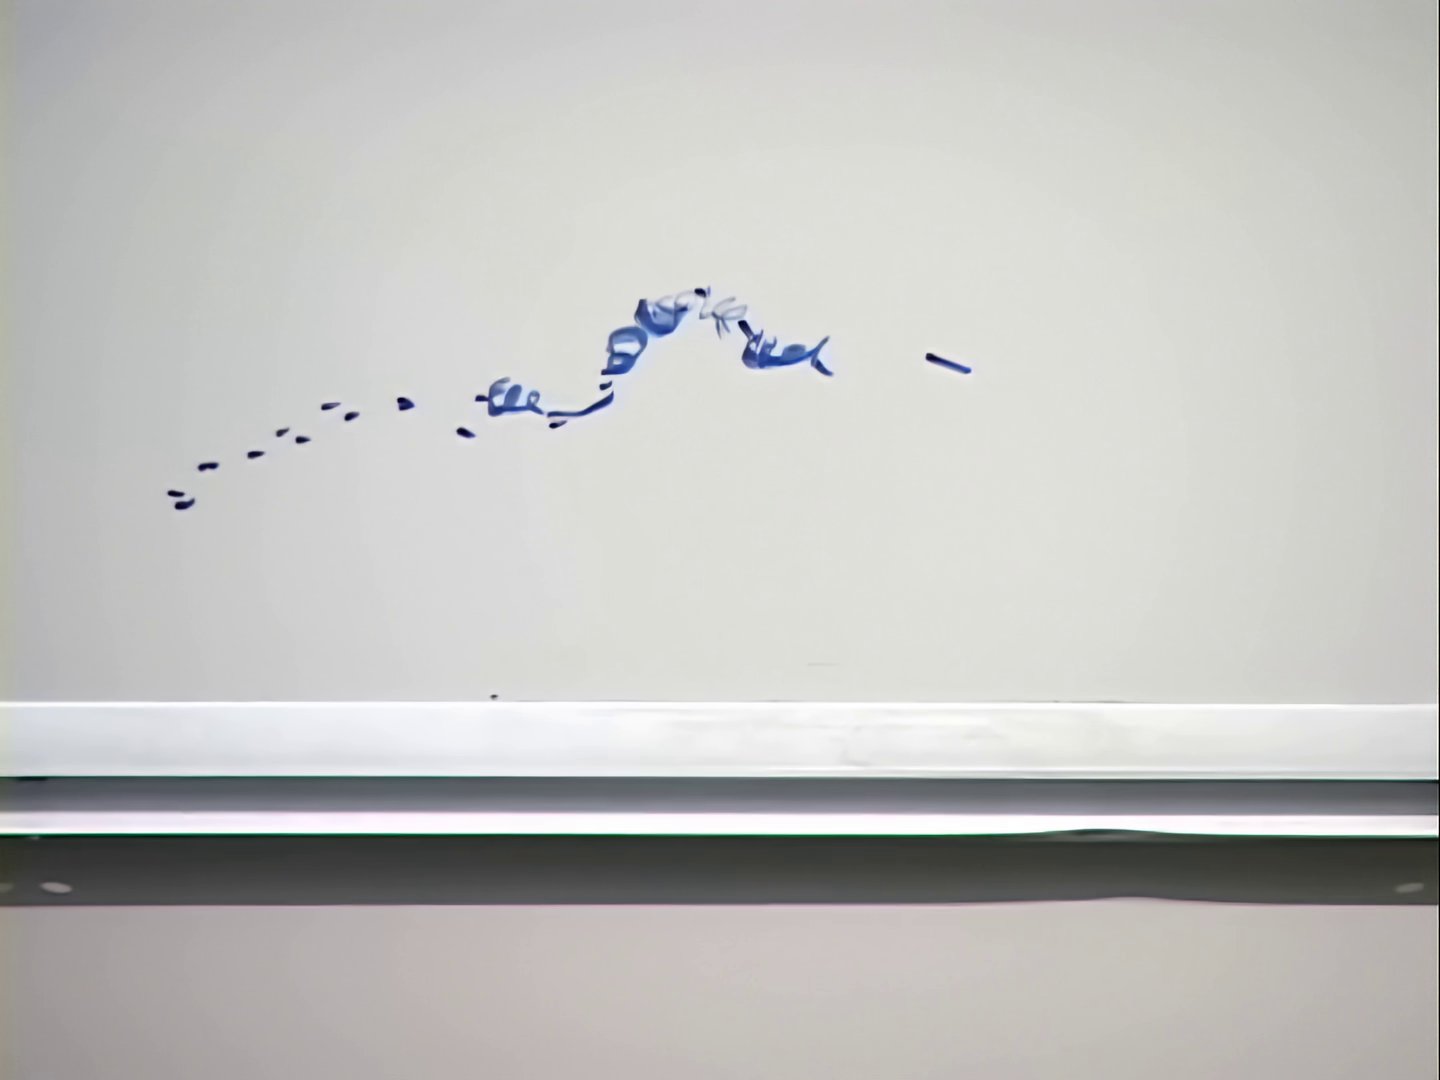
\includegraphics[width=0.75\textwidth]{lecture_01_figure_10.png}
  \caption{具有两个横向坐标的开弦的第一幅珠子-弹簧示意图。}
  \lectureframe{01:00:30}
  \label{fig:l01-bead-chain-board}
\end{figure}

\begin{figure}[H]
  \centering
  \begin{tikzpicture}[>=Latex]
    \foreach \x in {0,...,8} {
      \fill[blue!65!black] ({0.85*\x},0) circle (0.09);
    }
    \foreach \x in {0,...,7} {
      \draw[decorate,decoration={zigzag,segment length=4pt,amplitude=2pt}]
        ({0.85*\x+0.10},0) -- ({0.85*\x+0.75},0);
    }
    \draw[->] (3.4,0.15) -- (3.4,1.25) node[above] {$\bm X_i(t)$};
    \draw[<->] (0,-0.65) -- (6.8,-0.65)
      node[midway,below] {$0\leq\sigma\leq\pi$};
  \end{tikzpicture}
  \caption{开弦的离散正规化。在取连续极限之前，珠子质量和弹簧常数随间距缩放。}
  \label{fig:l01-bead-chain-redraw}
\end{figure}

\begin{figure}[H]
  \centering
  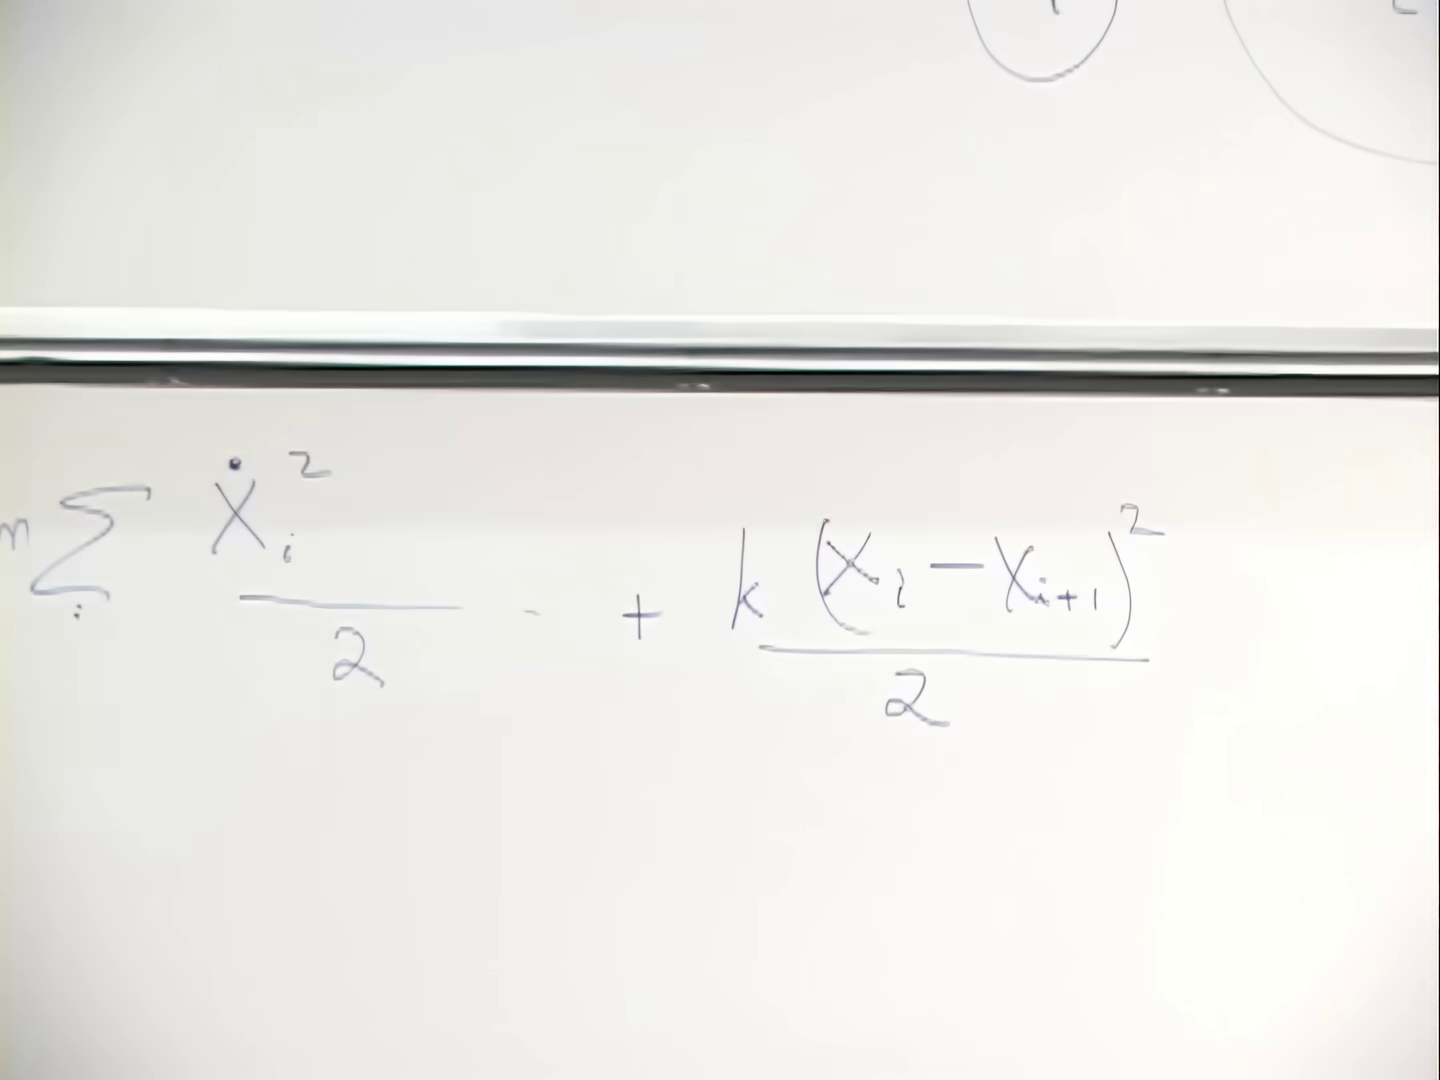
\includegraphics[width=0.78\textwidth]{lecture_01_figure_11.png}
  \caption{在取连续极限之前写在一起的离散动能项和胡克项。}
  \lectureframe{01:01:30}
  \label{fig:l01-discrete-energy-board}
\end{figure}

随着珠子数目的增加，每个珠子的质量 \(\mu_N\) 必须趋于零，以使整根弦保持有限的惯性。与此同时，弹簧常数 \(k_N\) 必须增大。一条长橡胶带比同种材料的一小段更容易被拉伸固定量；因此，如果连续材料要保持相同，被拉得更近的相邻点必须以更大的劲度相连。

引入沿弦的坐标 \(\sigma\)。其数值范围是一种约定。选择

\begin{equation}
  0\leq\sigma\leq\pi
\end{equation}

是方便的，因为闭弦之后可以从 \(0\) 参数化到 \(2\pi\)。求和变为积分，最近邻差分变为导数：

\begin{equation}
  \sum_i\longrightarrow\int_0^\pi d\sigma,
  \qquad
  \bm X_{i+1}-\bm X_i
  \longrightarrow
  \partial_\sigma\bm X.
  \label{eq:l01-continuum-replacements}
\end{equation}

在将依赖于间距的常数吸收进 \(t\)、\(\sigma\) 和 \(\bm X\) 的归一化之后，连续哈密顿量具有如下形式

\begin{equation}
  H_{\mathrm{string}}=
  \frac12\int_0^\pi d\sigma
  \left[
    \left(\partial_t\bm X\right)^2
    +\left(\partial_\sigma\bm X\right)^2
  \right].
  \label{eq:l01-continuum-hamiltonian}
\end{equation}

\begin{figure}[H]
  \centering
  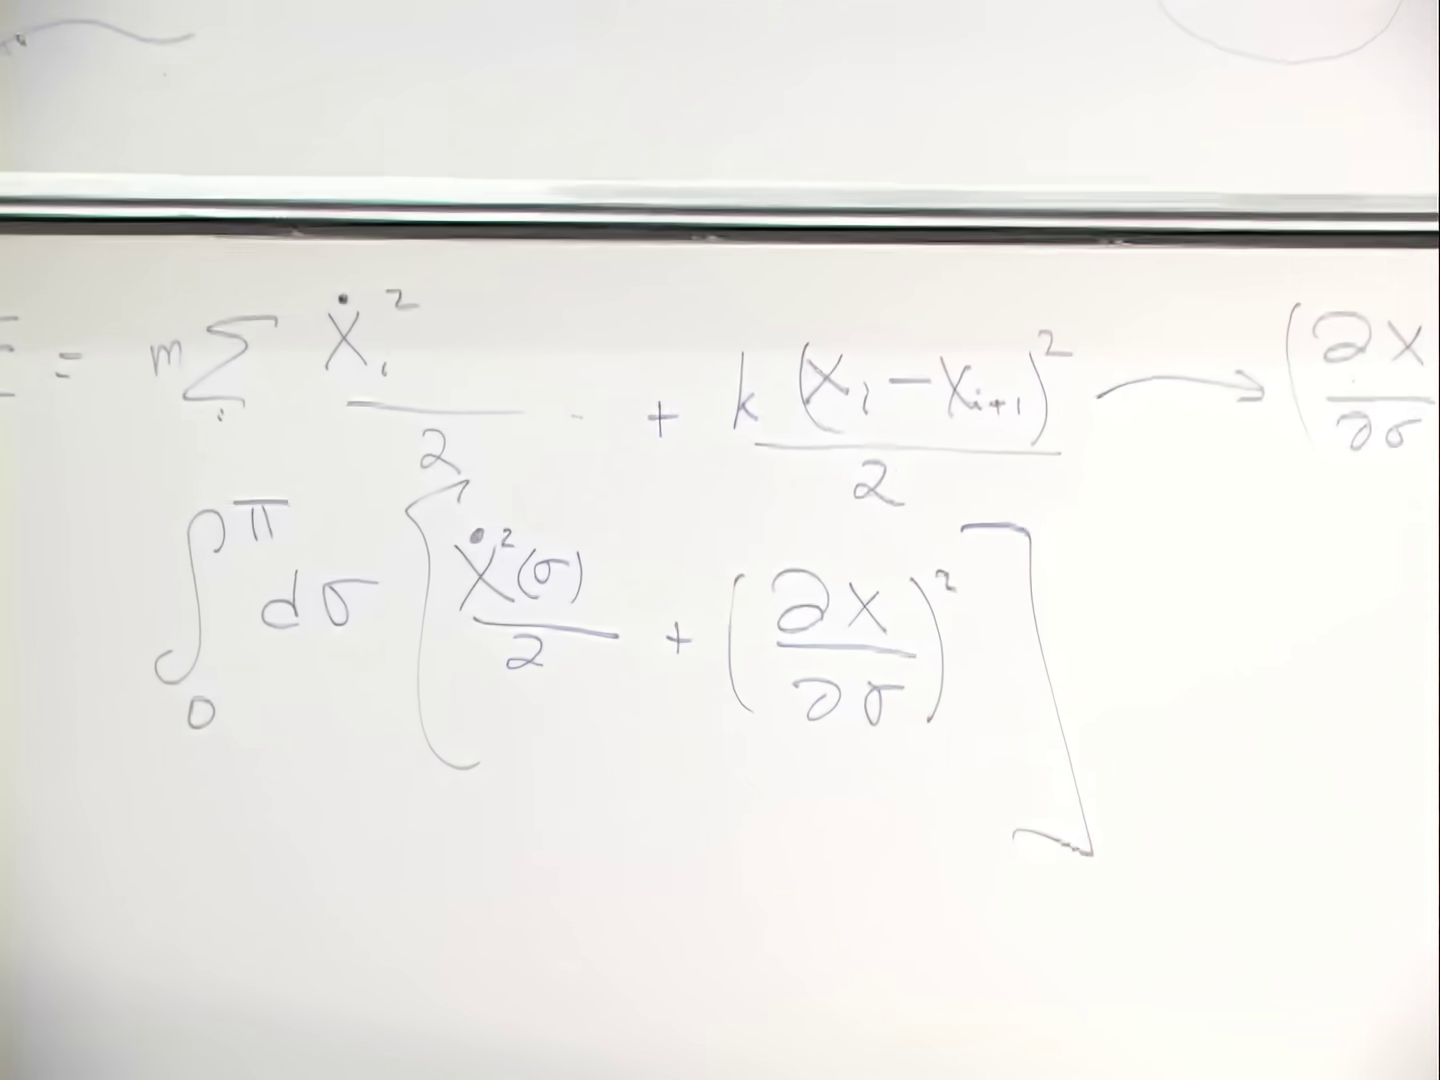
\includegraphics[width=0.78\textwidth]{lecture_01_figure_12.png}
  \caption{从珠子求和到 \(\int_0^\pi d\sigma\) 的板书推导过程，其中最近邻差分被替换为 \(\partial_\sigma\bm X\)。}
  \lectureframe{01:05:00}
  \label{fig:l01-continuum-board}
\end{figure}

第一项是两个横向方向上的动能。第二项度量沿弦的拉伸。两项都带正号，因为这是哈密顿量。在拉格朗日量中，势能项会以负号出现。精确的系数取决于约定，在此阶段尚未固定；真正重要的是动能加拉伸的结构。

将质心运动与相对运动分开。将每个点平移相同的量会使粒子整体移动。振荡、弯曲和相对拉伸是内部运动。质子、原子或任何其他复合物体都可以被称为粒子，即使其组分在内部运动。弦在这方面并无不同。

\section{为什么哈密顿量度量的是质量平方}

对于缓慢运动的物体，静能与其质量成正比。然而，在无穷动量描述中，内部贡献表现为 \(M^2/(2P_z)\)。一旦共同的纵向动量及其相关的时间重标度被固定，内部弦哈密顿量就与整个物体的不变质量平方成正比：

\begin{equation}
  H_{\mathrm{int}}\propto M^2.
  \label{eq:l01-hint-mass-squared}
\end{equation}

\editorialnote{更明确地说，光锥运动学给出形式为 \(M^2=2P^+P^- - \bm P_\perp^2\) 的不变关系。在质心横向参考系中且 \(P^+\) 固定时，光锥哈密顿量 \(P^-\) 因此与 \(M^2\) 成正比。本讲省略了这些归一化细节，只保留论证所需的比例关系。}

\begin{figure}[H]
  \centering
  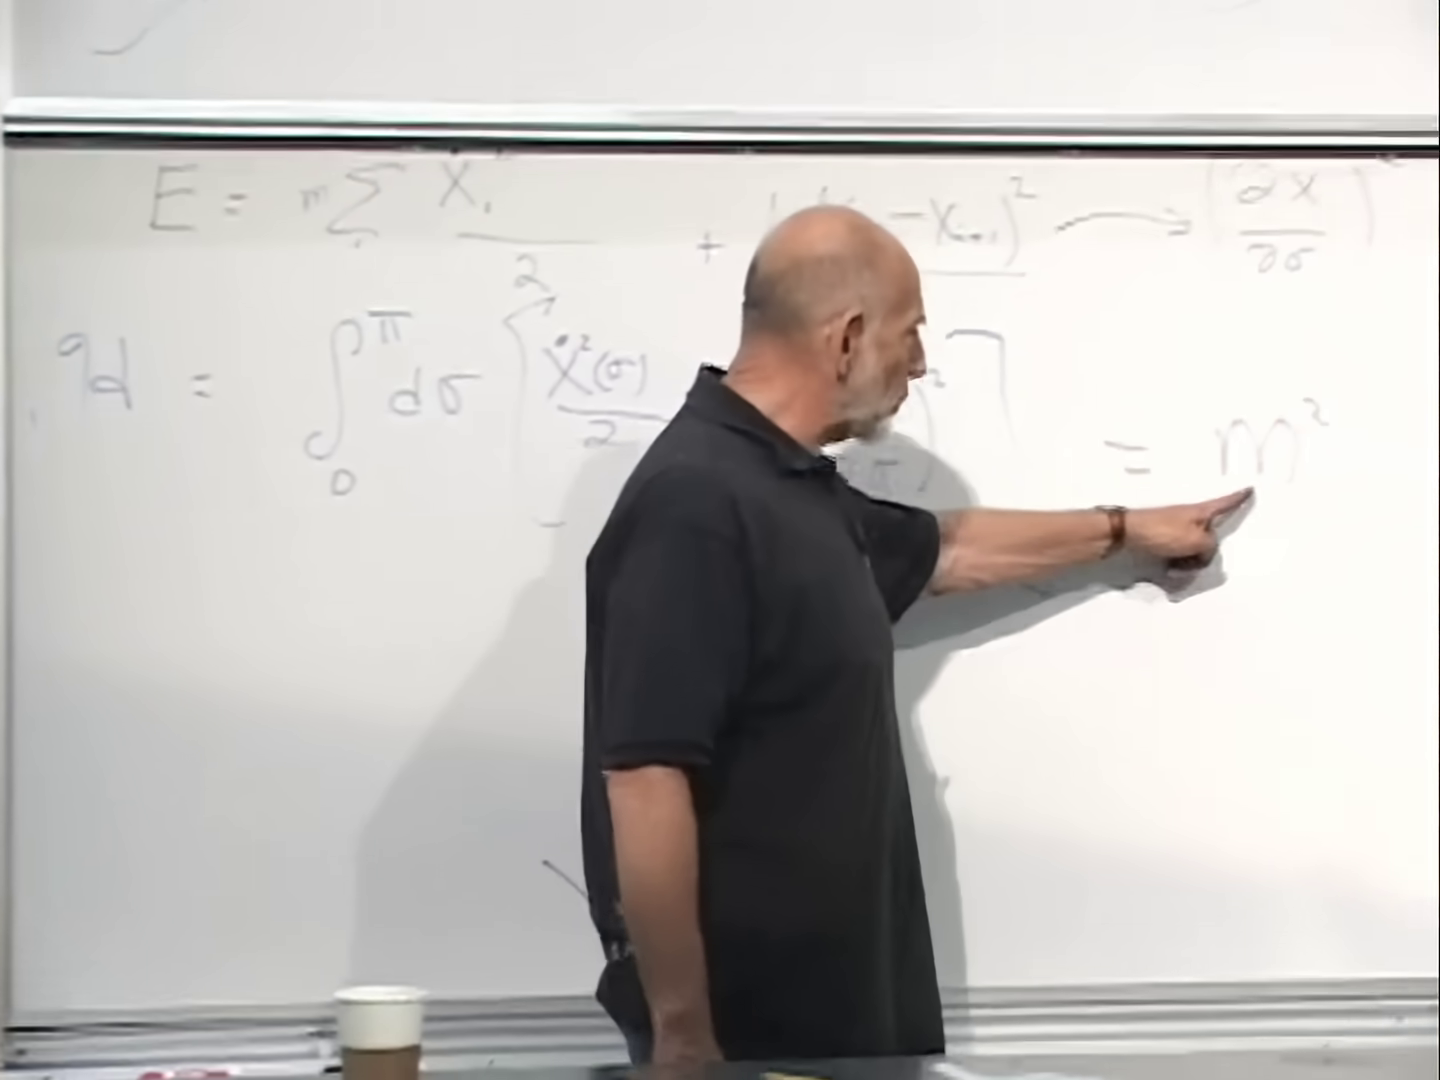
\includegraphics[width=0.76\textwidth]{lecture_01_figure_13.png}
  \caption{板书将内部弦能量等同于完整弦态的质量平方。}
  \lectureframe{01:10:30}
  \label{fig:l01-mass-squared-board}
\end{figure}

振动的弦是一组耦合振子。它的完整量子化被推迟了，但重要的谱结构事实已经可见。谐振子的能量以离散的台阶上升。由于这些内部能量对\(M^2\)有贡献，弦的激发自然会在质量平方中产生离散的台阶。这正是雷吉图在开头所预示的结构。

\begin{classroomqa}
\audiencequestion{\(M\)是整个弦的质量吗？如果将该质量加倍，相应的\(M^2\)贡献会变成四倍吗？
\lecturetimestamp{01:12:10}}
\lecturerresponse{是的。\(M\)是完整弦态的静止质量，包括振动、拉伸以及所有其他内部贡献。有效助推哈密顿量正比于\(M^2\)，因此质量加倍的态具有四倍的质量平方值。}
\end{classroomqa}

\begin{classroomqa}
\audiencequestion{这个描述如何能包含静止质量为零的光子？\lecturetimestamp{01:12:52}}
\lecturerresponse{无质量态对应于\(M=0\)。正的振子贡献如何能组合产生这样的态，是量子化理论的一个重要问题，而不是这里的经典模型所能解决的。在这一点上，\(M\)仅仅表示总静止质量，而量子力学尚未被引入。}
\end{classroomqa}

现在将一根不动的弦均匀拉伸到物理长度\(L\)。动能项消失，而在长度为\(\pi\)的参数区间上，

\begin{equation}
  \left|\partial_\sigma\bm X\right|\simeq\frac{L}{\pi}.
\end{equation}

因此，

\begin{align}
  H_{\mathrm{stretch}}
  &\propto
  \int_0^\pi d\sigma
    \left(\partial_\sigma\bm X\right)^2
  \notag\\
  &\simeq
  \pi\left(\frac{L}{\pi}\right)^2
  \propto L^2.
  \label{eq:l01-hooke-l2}
\end{align}

\begin{figure}[H]
  \centering
  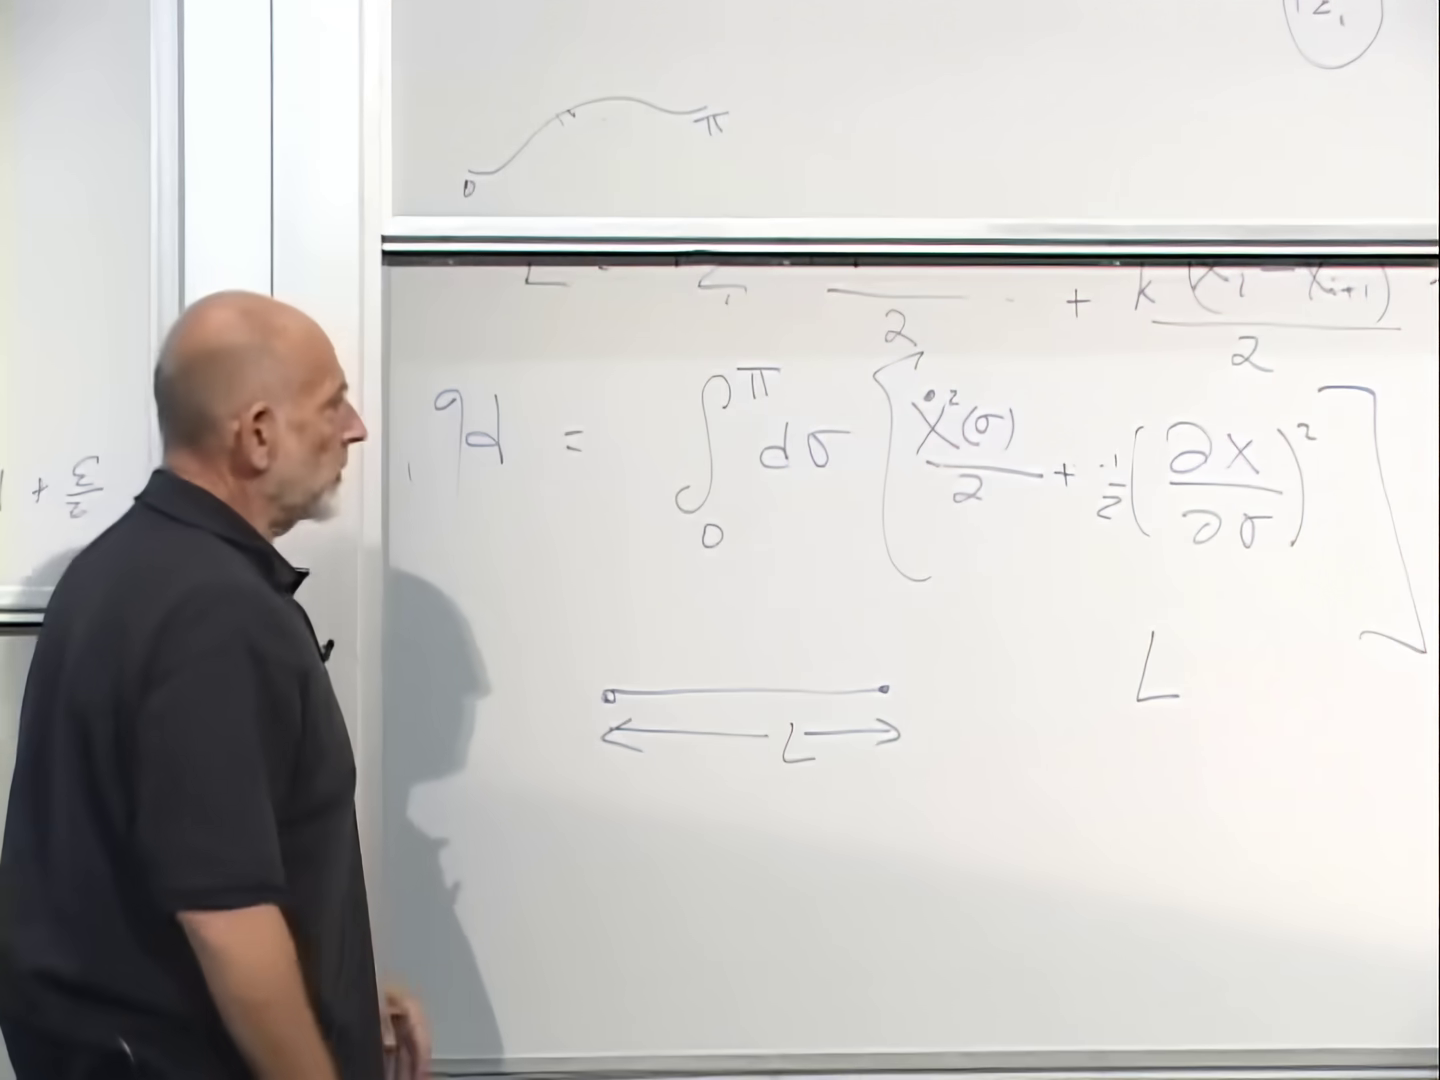
\includegraphics[width=0.76\textwidth]{lecture_01_figure_14.png}
  \caption{用于推断\(H_{\mathrm{stretch}}\propto L^2\)并进而推断\(M\propto L\)的均匀拉伸构型。}
  \lectureframe{01:15:30}
  \label{fig:l01-length-relation-board}
\end{figure}

这是有效横向力学中的胡克定律行为。但左边的量正比于\(M^2\)，而不是\(M\)。由此可得

\begin{equation}
  M^2\propto L^2,
  \qquad
  M\propto L.
  \label{eq:l01-mass-length}
\end{equation}

在静止系中能量为\(E_{\mathrm{rest}}=M\)，单位取\(c=1\)。将比例常数写为弦张力\(T\)，

\begin{equation}
  E_{\mathrm{rest}}=TL.
  \label{eq:l01-string-tension}
\end{equation}

结果与通量管图像一致。均匀的电场或磁场携带均匀的能量密度。如果其通量被限制在固定截面的管中，每增加一个单位长度就增加相同的能量。等价地，在新打开的每个间隙中填入新自由度的组分图像具有固定的单位长度能量。弦张力就是该单位长度能量。

这个结论是间接的。它并不声称任意被驱动到相对论速度的橡皮筋会自动获得\(E=TL\)。论证从大助推所导致的横向非相对论描述开始，将其内部能量等同于\(M^2\)，然后才将结果转换回静止系能量。

\section{同一物体在两个参考系中}

\(M\)与\(M^2\)之间的区别很容易被混淆，因此值得将两个展开式并排放置。取\(c=1\)，

\begin{align}
  E&=\sqrt{p^2+M^2}
  \simeq M+\frac{p^2}{2M},
  &&p\ll M,
  \label{eq:l01-rest-expansion-again}\\
  E&=\sqrt{P_z^2+M^2}
  \simeq P_z+\frac{M^2}{2P_z},
  &&P_z\gg M.
  \label{eq:l01-boost-expansion-again}
\end{align}

\begin{figure}[H]
  \centering
  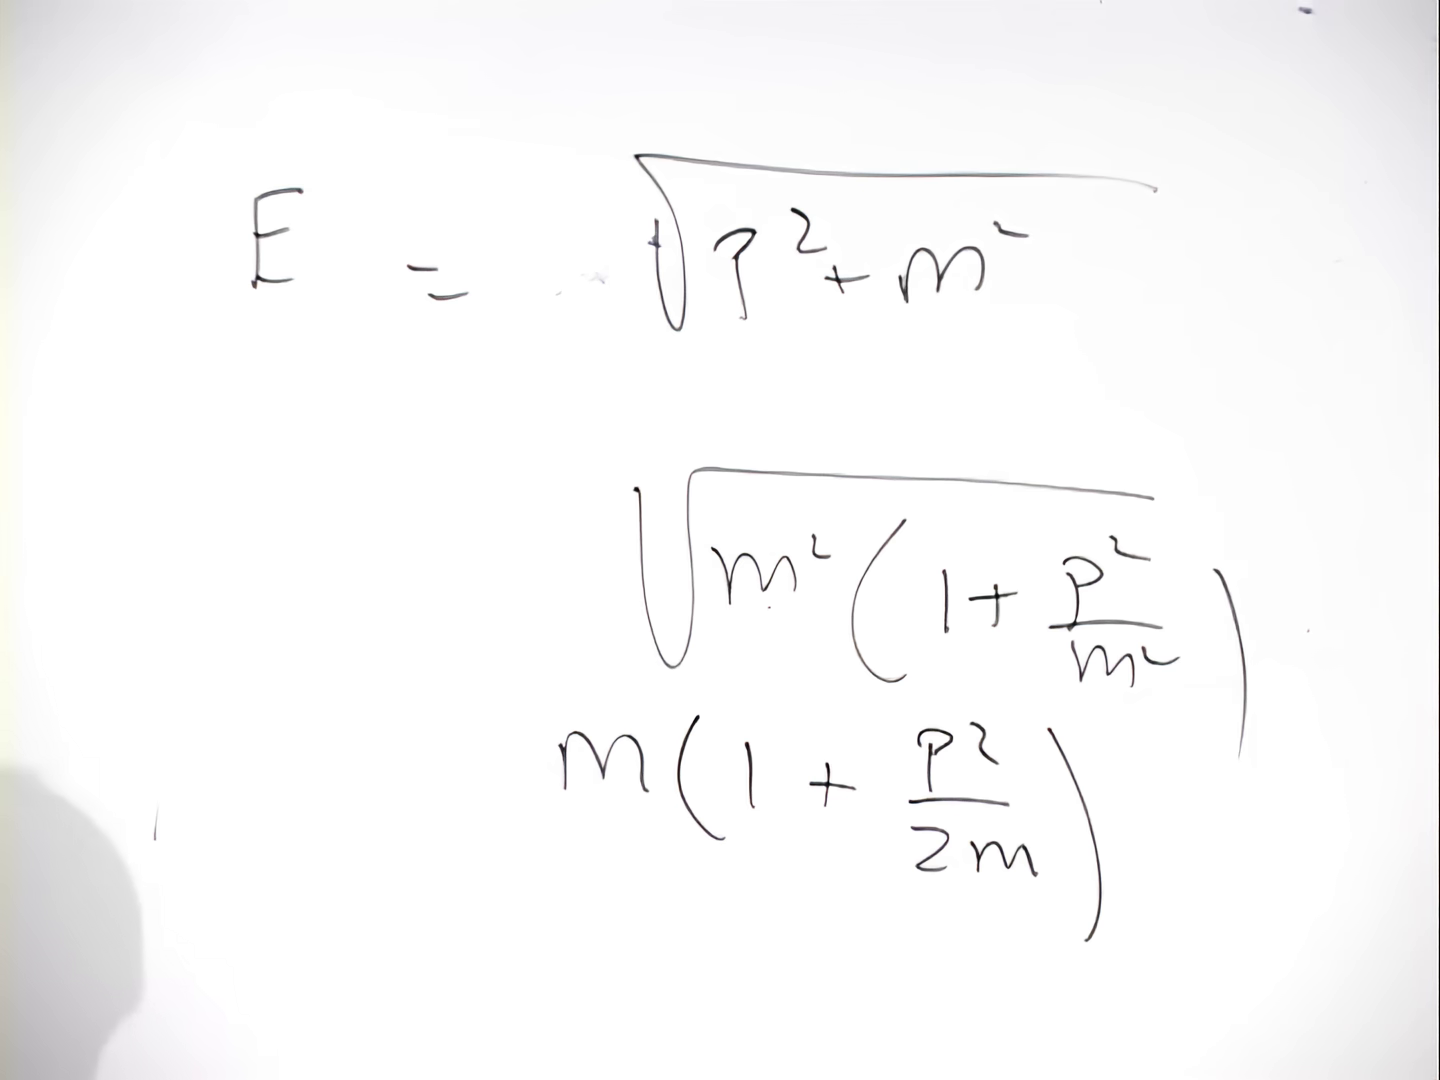
\includegraphics[width=0.74\textwidth]{lecture_01_figure_15.png}
  \caption{在分隔之后重复的小动量展开，其中内部静止能量被读作\(M\)。}
  \lectureframe{01:28:00}
  \label{fig:l01-rest-expansion-board-again}
\end{figure}

\begin{figure}[H]
  \centering
  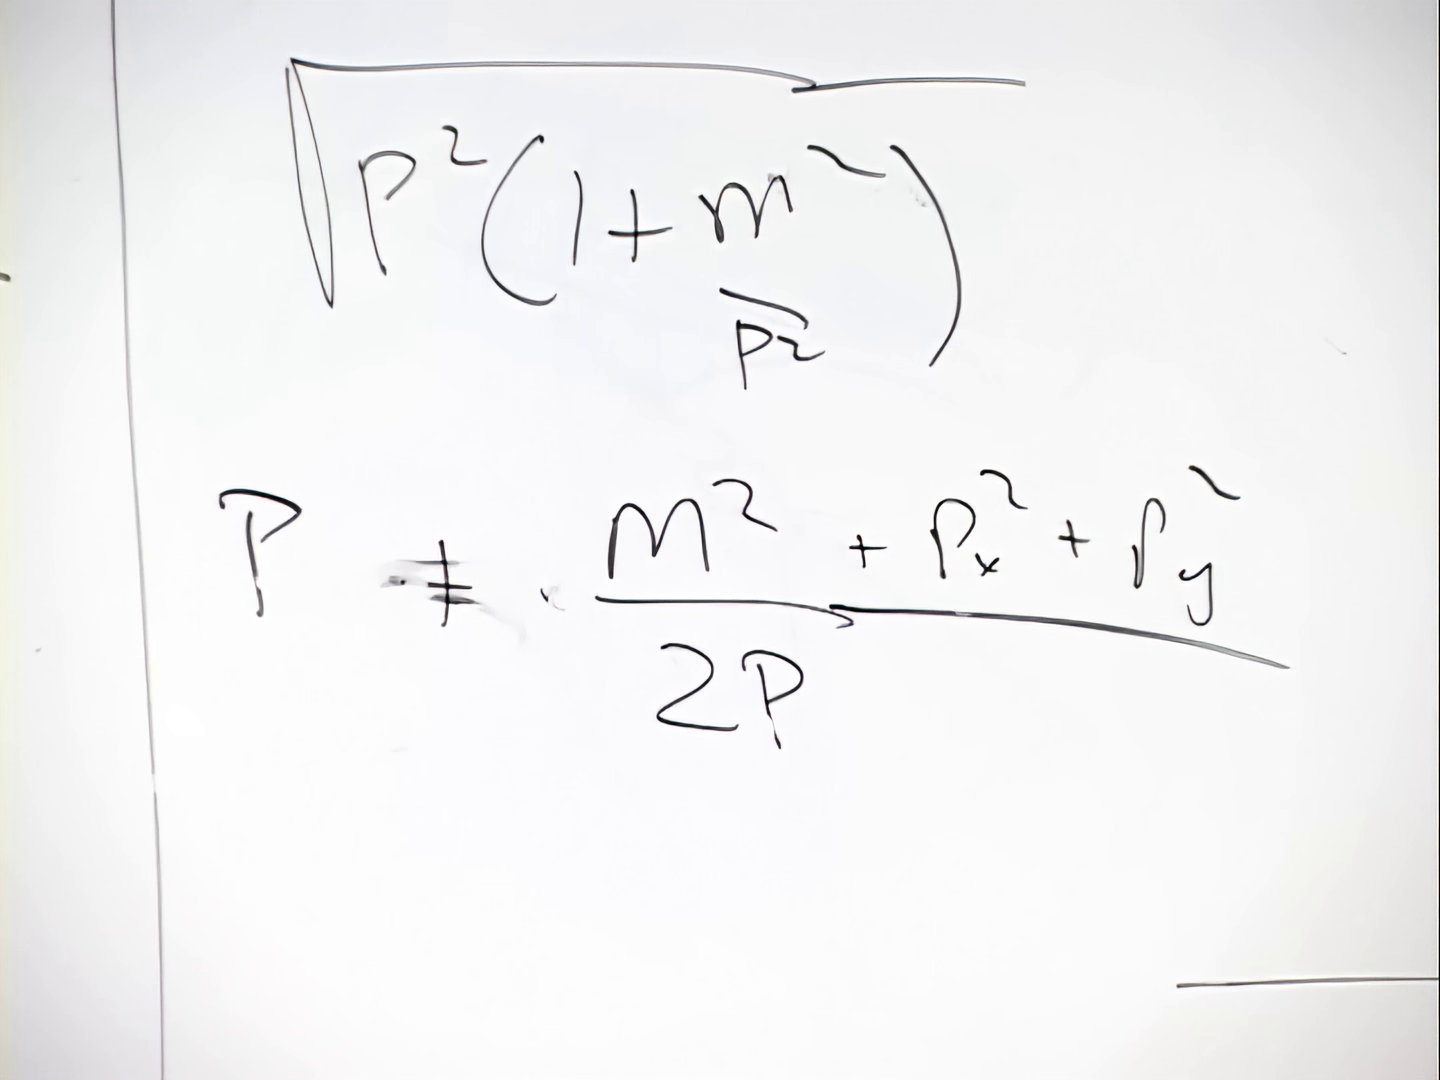
\includegraphics[width=0.74\textwidth]{lecture_01_figure_16.png}
  \caption{互补的大动量展开，其中剩余能量正比于\(M^2/(2P_z)\)。}
  \lectureframe{01:31:00}
  \label{fig:l01-boost-expansion-board-again}
\end{figure}

第一个展开将静止能量等同于质量，将普通惯性等同于\(M\)。在第二个展开中，守恒的\(P_z\)项被移除，横向惯性为\(P_z\)，内部能量由\(M^2/(2P_z)\)表示。无论在哪一个参考系中，质量都保持正比于弦长。变化的是质量的哪一个函数作为剩余哈密顿量出现。

\begin{classroomqa}
\audiencequestion{洛伦兹助推不应改变物理。为什么被助推的弦似乎服从不同的能量定律？
\lecturetimestamp{01:25:35}}
\lecturerresponse{它并不服从不同的物理。在两种描述中都有\(M\propto L\)和\(M^2\propto L^2\)。在静止系中，相关的能量是\(M\)；在大助推之后，守恒的\(P_z\)被分离出去，剩余的哈密顿量正比于\(M^2\)。助推改变的是有用的描述，而不是不变质量--长度关系。}
\end{classroomqa}

\section{一个超导的禁闭模型}

超导体将磁场从其体内排出。如果在材料变为超导态之前，磁通量被俘获在足够狭窄的通道中，那么磁通量就无法向侧面扩散，而是被限制在一根管中。一个有用的思想实验是：在正常态样品上钻一个窄孔，将一根长条形磁铁插入其中，冷却样品，然后抽出磁铁。这一构造是示意性的，而非实用的实验室操作方案。其目的是隔离出一条磁通线，使其场强和能量密度沿其长度方向近似均匀。

\begin{figure}[H]
  \centering
  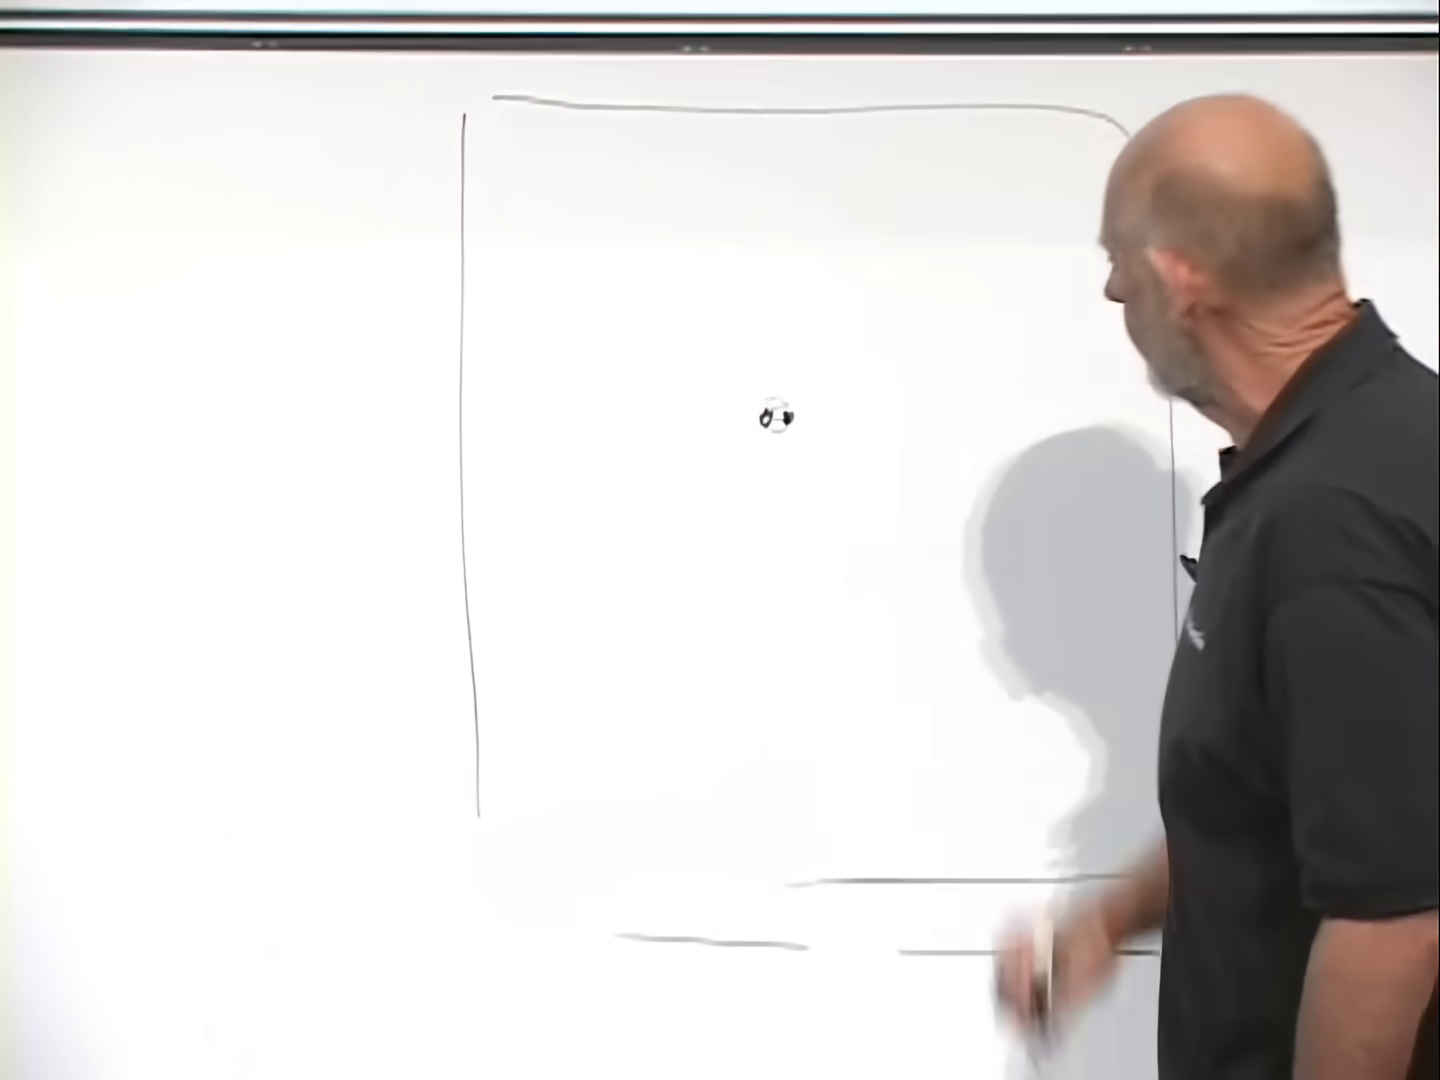
\includegraphics[width=0.76\textwidth]{lecture_01_figure_17.png}
  \caption{超导磁通线构造以及相应的单极子--反单极子禁闭图像。}
  \lectureframe{01:35:30}
  \label{fig:l01-superconductor-board}
\end{figure}

作为进一步的思想实验，假设可以将一个磁单极子和一个反单极子置于超导介质中并使其分离。它们之间的磁通量将被挤压成一根管。由于管每单位长度携带相同的能量，

\begin{equation}
  V(R)=T_{\mathrm{flux}}R.
  \label{eq:l01-linear-confinement}
\end{equation}

力 \(F=-dV/dR\) 的大小恒定。将这对粒子拉开变得越来越费力，因此这对粒子被禁闭。这正是人们为强子中的夸克所寻求的行为。

\begin{figure}[H]
  \centering
  \begin{tikzpicture}[>=Latex]
    \fill[blue!8,rounded corners=5pt] (-4,-1.35) rectangle (4,1.35);
    \node[blue!55!black] at (0,1.65) {superconducting medium};
    \fill[red!75!black] (-2.8,0) circle (0.17);
    \fill[blue!70!black] (2.8,0) circle (0.17);
    \node[below] at (-2.8,-0.22) {monopole};
    \node[below] at (2.8,-0.22) {antimonopole};
    \fill[orange!18,rounded corners=7pt] (-2.65,-0.42) rectangle (2.65,0.42);
    \draw[orange!85!black,thick,rounded corners=7pt]
      (-2.65,-0.42) rectangle (2.65,0.42);
    \foreach \y in {-0.22,0,0.22}
      \draw[->,orange!85!black] (-2.55,\y) -- (2.55,\y);
    \draw[<->] (-2.8,-1.00) -- (2.8,-1.00) node[midway,below] {$R$};
  \end{tikzpicture}
  \caption{磁通禁闭给出均匀的管和线性势
  \(V(R)=T_{\mathrm{flux}}R\)。}
  \label{fig:l01-superconductor-redraw}
\end{figure}

\begin{classroomqa}
\audiencequestion{在强子中，什么扮演了超导介质的角色？\lecturetimestamp{01:36:57}}
\lecturerresponse{所提出的类比将电和磁的角色互换。普通的超导凝聚体是带电的，并禁闭磁通量。在QCD的对偶超导体图像中，色磁物体的凝聚体禁闭夸克的色电荷。这类物体不会作为孤立粒子出现，因为它们被表示为凝聚在真空中。}
\end{classroomqa}

\editorialnote{对偶超导体描述是一种有影响力的禁闭机制，此处以讲座的历史性语言呈现。它应被理解为QCD真空的一种物理图像，而非从第一性原理出发对禁闭的完整推导。}

\begin{classroomqa}
\audiencequestion{能量与长度成正比，对于任何被高度相对论化的普通弦来说，这是一条普遍规则吗？\lecturetimestamp{01:38:10}}
\lecturerresponse{不是。人们首先需要一种关于该材料的自洽的相对论性理论，而其行为将取决于具体细节。线性能量是如下构型的特殊性质：其密度在被延伸时保持固定，或者磁通量被阻止横向扩散。将其拉开会产生更多的组分或更多均匀充满场的长度，而不仅仅是增大一组固定分子之间的间距。}
\end{classroomqa}

\section{横向自由度与粒子的尺度}

光锥构造直接以弦的横向坐标来书写弦。并不存在与每个横向振子相对应的、可独立指定的纵向振子。这种直接空间维度减少一个的现象是该形式体系的显著特征之一；不过，完整的理论仍必须满足洛伦兹不变性。

\begin{classroomqa}
\audiencequestion{沿 \(z\) 方向的剩余运动会发生什么？
\lecturetimestamp{01:40:10}}
\lecturerresponse{在光锥描述中，纵向运动不是作为独立自由度引入的。物理振荡由横向描述，而约束条件决定了纵向信息。这种经济性与如下想法在精神上相关：引力系统或许允许一种直接维度少一个的描述，尽管此处并未推导这一联系。}
\end{classroomqa}

\begin{classroomqa}
\audiencequestion{雷吉图上实际已知多少个点？
\lecturetimestamp{01:41:15}}
\lecturerresponse{确切的最大值取决于家族；粗略的数字大约是七个。这一序列在实验上并非无穷无尽。相关的事实是，已知的点并未显示出普通宏观材料中那种可见的失效或断裂端点。}
\end{classroomqa}

强子现象学提供了历史动机，但数学弦理论并不需要复现强子的每一个细节。一旦形式体系建立起来，人们就会问它实际上描述了什么。它的无质量自旋二态和其他性质更自然地指向引力。

强子与电子之间的表面差异可以用刚性转动的能量来量化，

\begin{equation}
  E_{\mathrm{rot}}=\frac{J^2}{2I},
  \qquad
  I\sim MR^2.
  \label{eq:l01-rotational-energy}
\end{equation}

角动量是量子化的。将 \(J^2\) 示意性地写作 \(\hbar^2 n^2\)，第一个转动台阶的量级为

\begin{equation}
  \Delta E_{0\to1}\sim\frac{\hbar^2}{2I}.
  \label{eq:l01-first-rotational-step}
\end{equation}

\begin{figure}[H]
  \centering
  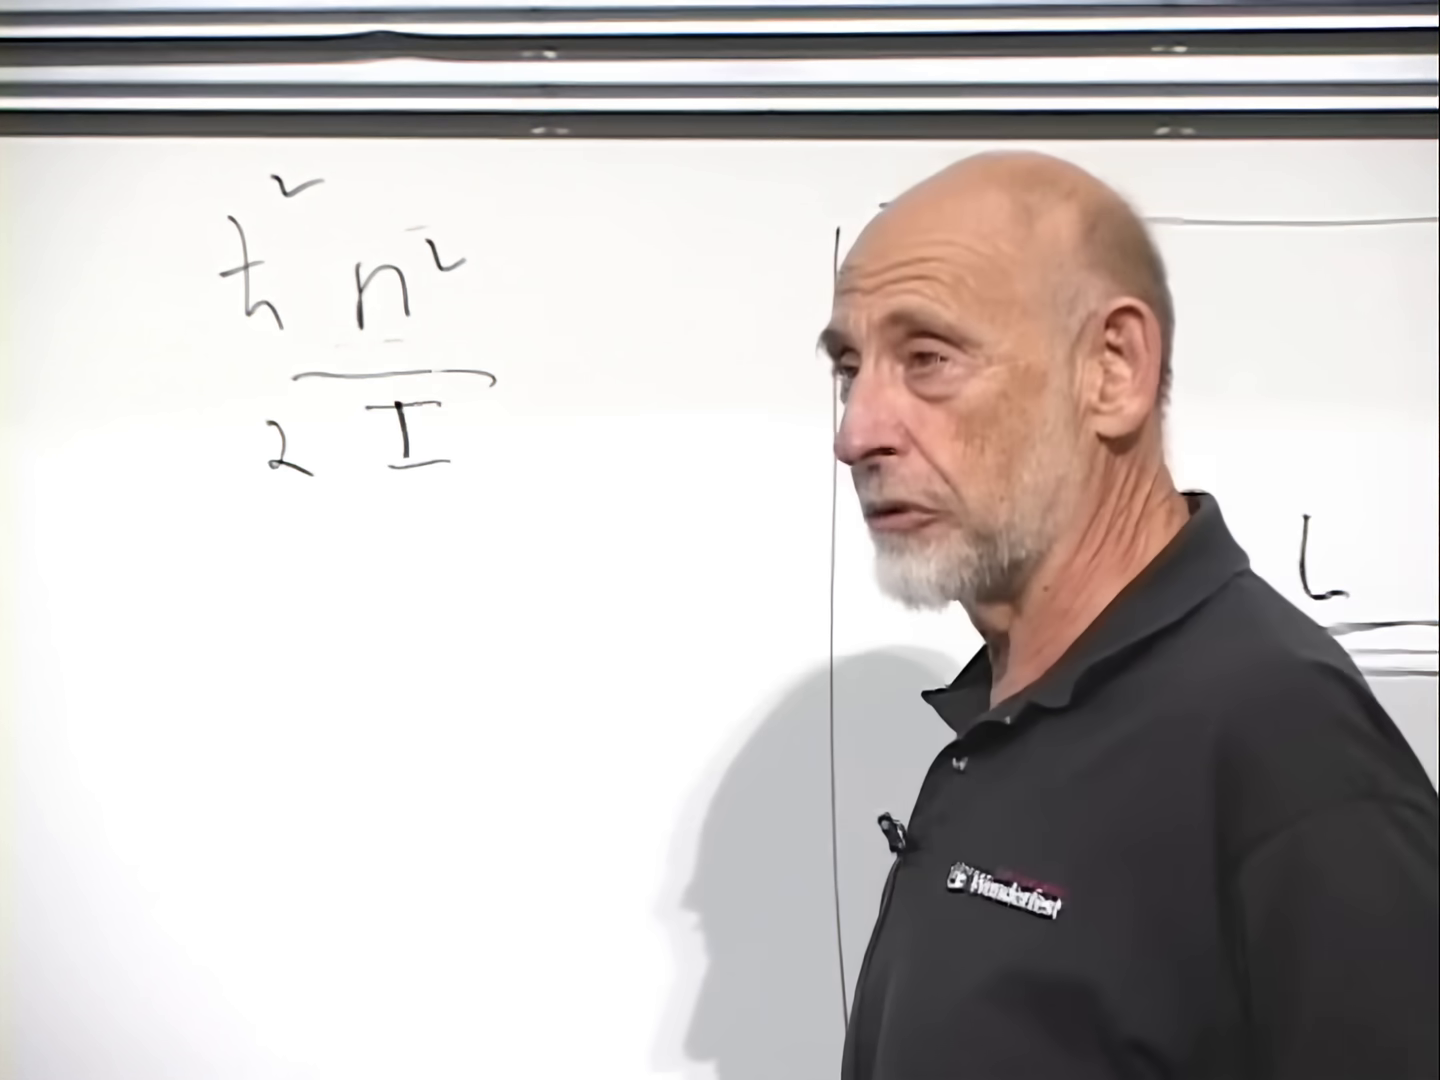
\includegraphics[width=0.76\textwidth]{lecture_01_figure_18.png}
  \caption{第一转动激发的转动惯量估计，\(\Delta E\sim\hbar^2/(2I)\)。}
  \lectureframe{01:44:00}
  \label{fig:l01-rotational-board}
\end{figure}

对于固定质量，半径越小意味着转动惯量小得多，而激发能量大得多。强子在自身内部动力学的尺度上很大，因此一次转动激发大约需要一GeV的能量，在粒子碰撞中是可以达到的。如果电子具有任何空间子结构，实验限制使其尺度远小于此，而转动激发将远超出可获得的能量范围。篮球则处于相反的极端：其转动惯量如此之大，以至于一个角动量量子所需的能量小得无法察觉。原子的转动或轨道能级跃迁介于这些极端之间，通常在电子伏特的量级。

\begin{classroomqa}
\audiencequestion{一个看似基本的电子是否仍可能具有空间结构和转动激发？\lecturetimestamp{01:42:04}}
\lecturerresponse{它只能将它们隐藏在非常高的能量处。一个单位角动量的代价按\(1/I\)标度，而\(I\sim MR^2\)。因此，极小的半径会将第一激发推到质量平方图上很远的地方。未观察到电子激发意味着，要么电子是点状的，要么任何复合尺度都远小于当前实验所能分辨的尺度。}
\end{classroomqa}

现在可以从动力学角度解读开篇的Regge图。强子之所以展现出可及的转动和振动状态，是因为它们是延展的。其质量平方谱中的等间距步长，正是将振子哈密顿量等同于\(M^2\)时所预期的特征。其能量随长度近似线性变化，是恒定张力通量管的特征。光谱学、散射对偶性、世界面几何和光锥力学，是对同一个组织性思想的四种描述：一个延展的相对论性客体，其自然的内部变量是质量平方。

\chapter{从边界条件到开弦谱}

\lectureoverview{我们的目标是量子化一根开弦，并判定它的态是否配得上被称为粒子。这条路线是初等的，但要求严格。我们首先准备 \(0\leq\sigma\leq\pi\) 上函数的微积分与傅里叶分析。随后，我们用粒子行为的谱判据取代点状性，回顾横向动力学变为非相对论性的无限动量描述，并用一链轻质量与刚性弹簧构造弦。连续弦是一个具有自由端点的波动系统。它的诺伊曼模解耦为频率为 \(1,2,3,\ldots\) 的谐振子；因此量子化产生离散的、有能隙的谱。弦的相互作用最终迫使我们超出开弦：一根开弦可以把自己的端点连接起来而变成闭弦。}

\section{开弦区间上的微积分}

计算将反复把离散求和变为积分，把最近邻差分变为导数。最好在它们打断物理讨论之前先把这些事实准备好。

设 \(x(\sigma)\) 是定义在

\begin{equation}
  0\leq \sigma\leq \pi .
\end{equation}

记号已经预示了弦论：\(\sigma\) 标记沿弦的位置，而 \(x\) 将成为它的一个横向坐标。把区间分成 \(N\) 段，

\begin{equation}
  \Delta\sigma=\frac{\pi}{N},
  \qquad
  \sigma_i=i\,\Delta\sigma,
  \qquad
  x_i=x(\sigma_i).
  \label{eq:l02-lattice}
\end{equation}

对于光滑的极限函数，

\begin{equation}
  \Delta x_i\equiv x_i-x_{i-1}
  =
  \frac{\partial x}{\partial\sigma}\,\Delta\sigma
  +O\!\left((\Delta\sigma)^2\right),
  \label{eq:l02-difference}
\end{equation}

而黎曼和变为

\begin{equation}
  \sum_i x_i\,\Delta\sigma
  \longrightarrow
  \int_0^\pi x(\sigma)\,d\sigma .
  \label{eq:l02-riemann}
\end{equation}

\begin{figure}[H]
  \centering
  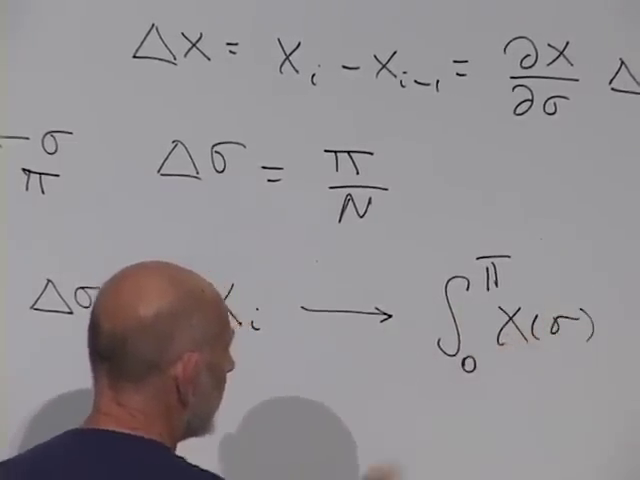
\includegraphics[width=0.78\textwidth]{lecture_02_figure_01.png}
  \caption{为后续连续极限保留在黑板上的有限差分与黎曼和规则。}
  \lectureframe{00:04:20}
  \label{fig:l02-calculus-board}
\end{figure}

这些都是微积分中熟悉的定义。它们在这里的重要性在于标度：\(\Delta x_i\) 带来一个 \(\Delta\sigma\) 的幂，而一个求和变为积分时则带来一个逆幂。

\subsection{狄利克雷端点与诺伊曼端点}

有限区间上的傅里叶分析始于端点处的一种选择。有两种选择会反复出现。

\begin{align}
  \text{Dirichlet:}\qquad
  &x(0)=x(\pi)=0,
  \label{eq:l02-dirichlet}\\
  \text{Neumann:}\qquad
  &\left.\partial_\sigma x\right|_{\sigma=0}
   =
   \left.\partial_\sigma x\right|_{\sigma=\pi}
   =0.
  \label{eq:l02-neumann}
\end{align}

两端被固定的提琴弦给出狄利克雷图像：其位移在边界处为零。诺伊曼函数则不必在边界处为零；它以零斜率与每个边界相接。这两种特征形状一起显示在黑板上。

\begin{figure}[H]
  \centering
  \begin{minipage}[t]{0.48\textwidth}
    \centering
    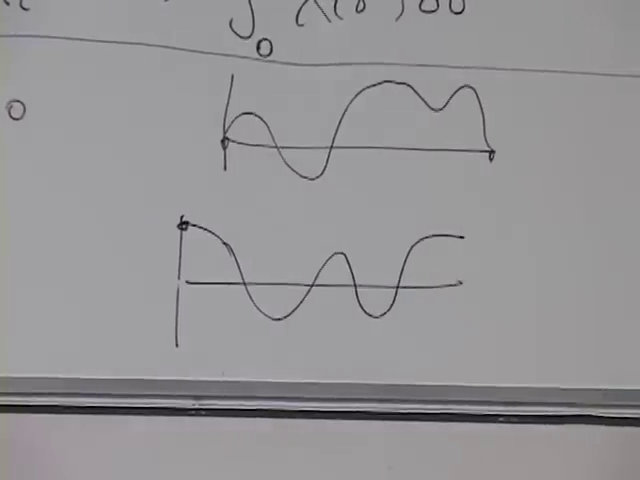
\includegraphics[width=\textwidth]{lecture_02_figure_02.png}
    \par\smallskip\footnotesize (a) 被钉住且平坦的端点剖面。
  \end{minipage}\hfill
  \begin{minipage}[t]{0.48\textwidth}
    \centering
    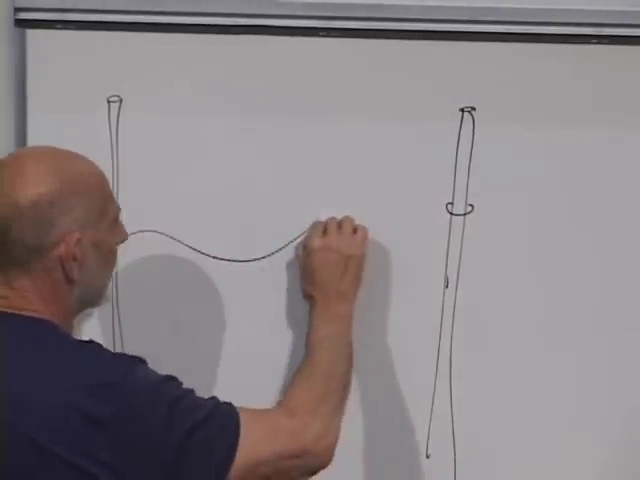
\includegraphics[width=\textwidth]{lecture_02_figure_03.png}
    \par\smallskip\footnotesize (b) 在竖直杆上滑动的轻环。
  \end{minipage}
  \caption{作为形状与力学的边界条件。滑动环构造赋予自由端点一个明确的横向运动。}
  \lectureframe{00:08:50 and 00:12:15}
  \label{fig:l02-boundaries-board}
\end{figure}

\begin{figure}[H]
  \centering
  \begin{adjustbox}{max width=\linewidth}
  \begin{tikzpicture}[>=Latex,thick,scale=0.92]
    \begin{scope}
      \draw[->] (0,0) -- (4.4,0) node[right] {\(\sigma\)};
      \draw[->] (0,-1.25) -- (0,1.35) node[above] {\(x\)};
      \draw[blue!70!black]
        (0,0) .. controls (0.8,1.1) and (1.4,1.0) .. (2.0,0)
        .. controls (2.7,-1.0) and (3.4,-0.8) .. (4.1,0);
      \fill (0,0) circle (0.06);
      \fill (4.1,0) circle (0.06);
      \node at (2.05,-1.65) {Dirichlet: \(x=0\)};
    \end{scope}
    \begin{scope}[xshift=5.8cm]
      \draw[->] (0,0) -- (4.4,0) node[right] {\(\sigma\)};
      \draw[->] (0,-1.25) -- (0,1.35) node[above] {\(x\)};
      \draw[orange!85!black]
        (0,0.65) .. controls (0.8,0.65) and (1.1,-0.9) .. (2.0,-0.9)
        .. controls (2.9,-0.9) and (3.2,0.55) .. (4.1,0.55);
      \draw[orange!85!black] (0,0.65) -- (0.45,0.65);
      \draw[orange!85!black] (3.65,0.55) -- (4.1,0.55);
      \node at (2.05,-1.65) {Neumann: \(\partial_\sigma x=0\)};
    \end{scope}
  \end{tikzpicture}
  \end{adjustbox}
  \caption{对于狄利克雷数据，函数值固定；对于诺伊曼数据，斜率固定。}
  \label{fig:l02-boundaries-redraw}
\end{figure}

\begin{classroomqa}
\audiencequestion{开管或闭管风琴能否为这些边界条件之一提供一个清晰的例子？\lecturetimestamp{00:09:19}}
\lecturerresponse{可以，但首先必须说明正在展开的是哪个声学变量。压力扰动与纵向位移在开口端服从互补的理想化条件。与其在黑板上解决这个枝节问题，不如使用滑动环模型：近乎无质量的环可以在杆上竖直移动，因此弦的端点是自由的，诺伊曼图像是直接的。}
\end{classroomqa}

\begin{classroomqa}
\audiencequestion{图像能否竖直上升并包含一个尖锐的跳跃？\lecturetimestamp{00:09:53}}
\lecturerresponse{傅里叶分析允许分段连续函数中存在孤立跳跃。物理弦则更具限制性。一个跳跃会断开相邻点，并使空间导数 \(\partial_\sigma x\) 在下面导出的连续能量中奇异。因此我们只关注连续且可微的剖面。}
\end{classroomqa}

\begin{classroomqa}
\audiencequestion{为什么管子的开口端，或任何自由端，竟然要满足边界条件？\lecturetimestamp{00:11:14}}
\lecturerresponse{声学例子取决于所选的场，在讨论中未得到解决。力学例子则不然。一个非常轻的环可以自由滑动，但仍然连接在最后一段弦上。我们将从牛顿定律推导它的条件，而不是假设它：有限的端点加速度迫使斜率消失。}
\end{classroomqa}

\subsection{傅里叶基}

一旦端点类别固定，相应的傅里叶基也就固定。在 \(0\leq\sigma\leq\pi\) 上，

\begin{align}
  x_D(\sigma)
  &=
  \sum_{n=1}^{\infty}x_n\sin(n\sigma),
  \label{eq:l02-dirichlet-series}\\
  x_N(\sigma)
  &=
  \sum_{n=0}^{\infty}x_n\cos(n\sigma).
  \label{eq:l02-neumann-series}
\end{align}

\eqref{eq:l02-dirichlet-series} 中的每个正弦都在两个端点处为零。
\eqref{eq:l02-neumann-series} 中的每个余弦都有零端点导数。
下限不同是有原因的：
\(\sin(0\sigma)=0\) 不贡献任何东西，而
\(\cos(0\sigma)=1\) 是常数模，或零模。它记录诺伊曼函数的平均值。

\begin{figure}[H]
  \centering
  \begin{minipage}[t]{0.48\textwidth}
    \centering
    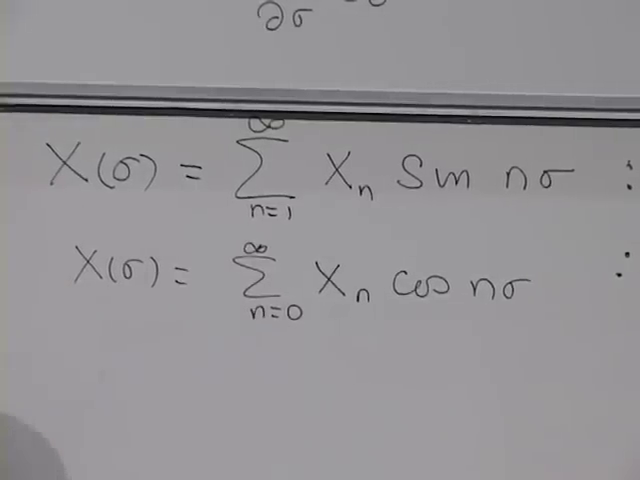
\includegraphics[width=\textwidth]{lecture_02_figure_04.png}
    \par\smallskip\footnotesize (a) 正弦与余弦展开。
  \end{minipage}\hfill
  \begin{minipage}[t]{0.48\textwidth}
    \centering
    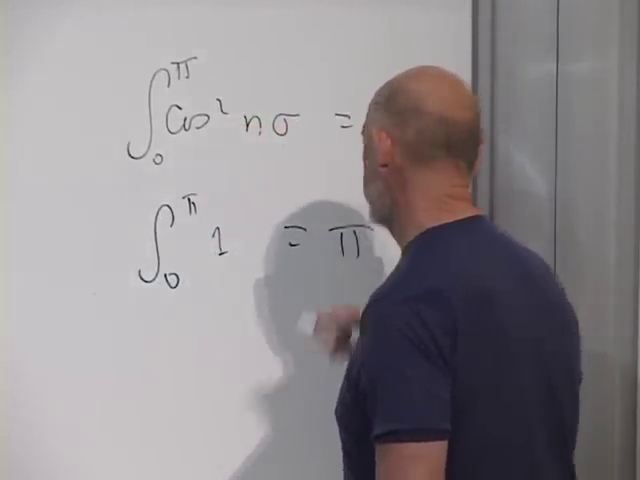
\includegraphics[width=\textwidth]{lecture_02_figure_05.png}
    \par\smallskip\footnotesize (b) 正交性与例外的
    常数模式。
  \end{minipage}
  \caption{后文用于将弦对角化的傅里叶事实。}
  \lectureframe{00:16:15 and 00:20:30}
  \label{fig:l02-fourier-board}
\end{figure}

求导交换这两类：

\begin{equation}
  \begin{aligned}
    \partial_\sigma\sin(n\sigma)&=n\cos(n\sigma),\\
    \partial_\sigma\cos(n\sigma)&=-n\sin(n\sigma).
  \end{aligned}
  \label{eq:l02-basis-derivatives}
\end{equation}

因此，Dirichlet 级数的导数具有 Neumann 行为，而 Neumann 级数的导数具有 Dirichlet 行为。正交性随后消去不同模式之间的交叉项：

\begin{align}
  \int_0^\pi\cos(n\sigma)\cos(m\sigma)\,d\sigma
  &=
  \frac{\pi}{2}\delta_{nm},
  && n,m\geq1,
  \label{eq:l02-cos-orthogonality}\\
  \int_0^\pi\sin(n\sigma)\sin(m\sigma)\,d\sigma
  &=
  \frac{\pi}{2}\delta_{nm},
  && n,m\geq1,
  \label{eq:l02-sin-orthogonality}\\
  \int_0^\pi 1\,d\sigma&=\pi .
  \label{eq:l02-zero-norm}
\end{align}

最后一行是例外的 \(n=m=0\) 余弦范数。常数并不像非零谐波那样被归一化，而那个因子二将把弦的质心模式与其内部模式区分开来。

\subsection{一个要记住的振子公式}

在重新标度坐标使其力学质量为 1 之后，胡克定律振子有

\begin{align}
  E_{\mathrm{osc}}
  &=
  \frac12\dot q^{\,2}
  +\frac12\omega^2q^2,
  \label{eq:l02-oscillator-energy}\\
  L_{\mathrm{osc}}
  &=
  \frac12\dot q^{\,2}
  -\frac12\omega^2q^2.
  \label{eq:l02-oscillator-lagrangian}
\end{align}

\begin{figure}[H]
  \centering
  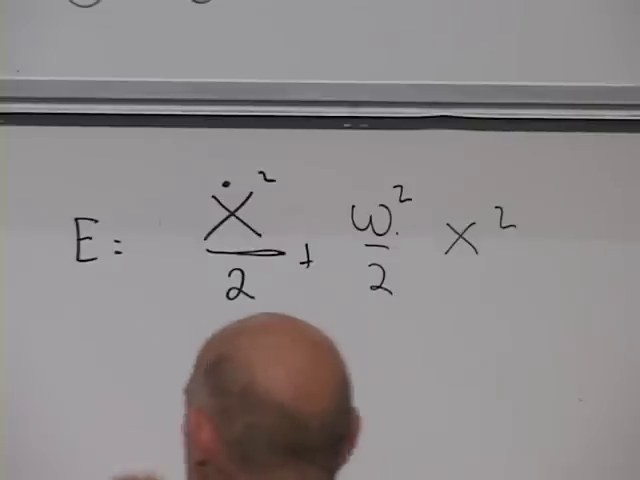
\includegraphics[width=0.68\textwidth]{lecture_02_figure_06.png}
  \caption{振子能量，如此写出使得 \(q^2\) 的系数
  立即标识出 \(\omega^2\)。}
  \lectureframe{00:24:00}
  \label{fig:l02-oscillator-board}
\end{figure}

经典地，\(\omega=\sqrt{\kappa/m}\)；坐标的重新标度已设定
\(m=1\)。量子力学地，

\begin{equation}
  E_Q=\hbar\omega\left(Q+\frac12\right),
  \qquad Q=0,1,2,\ldots .
  \label{eq:l02-oscillator-spectrum}
\end{equation}

对于能级间距，我们可以减去共同的基态项，并说每个量子花费 \(\hbar\omega\)。弦的计算最初将恰好这样做，并推迟总零点能。

\begin{classroomqa}
\audiencequestion{如何从能量公式读出振子频率？\lecturetimestamp{00:23:21}}
\lecturerresponse{在重新标度之前它是
\(\omega=\sqrt{\kappa/m}\)。在单位质量下，势项为
\(\frac12\omega^2q^2\)，因此其二次系数就是频率的平方。}
\end{classroomqa}

\section{是什么使一个复合系统成为粒子？}

弦是延展的，并将由许多耦合的片段来建模。那么，在什么意义上它的一个量子态仍可以是粒子？点状性不能是决定性的判据。质子和中子是复合的。电子和光子即使没有分辨出任何内禀子结构，也伴随着量子场的缀饰。一个周围空无一物的经典几何点并不是量子激发的正确图像。

质量和质心位置也不充分。一个密封的气体盒子两者都有。一杯咖啡两者都有。我们通常不把其中任何一个称为粒子。不可分性也不成立，因为质子是可分的，而自旋并不区分微观粒子与宏观物体。

有用的判据是谱隔离。把静能放在竖直轴上，并问需要多少能量才能到达另一个内部态。电子在紧邻其上方没有实验上可及的电子激发塔。质子确实有共振，但最初的几个共振要花费几百 MeV，即质子质量的相当一部分。那些态被分隔得足够开，可以逐个辨认。

一杯咖啡则相反。人们可以向一个长波长声模式加入任意小的能量，轻推一个分子，或产生一个声子。有极多的态挤在一个微小的间隔内。在实验室尺度上，它们形成一个连续统。这就是粒子与 \emph{糊状物} 之间的实际区别。

\begin{figure}[H]
  \centering
  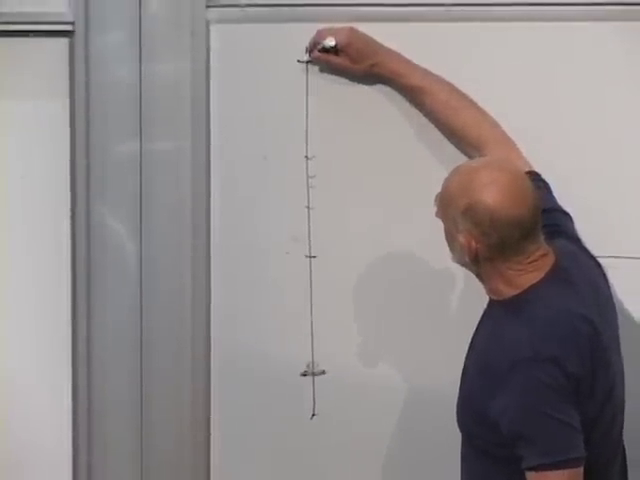
\includegraphics[width=0.58\textwidth]{lecture_02_figure_07.png}
  \caption{在比较孤立粒子能级与普通物质的密集激发时，黑板上的竖直能量轴。}
  \lectureframe{00:31:10}
  \label{fig:l02-spectrum-board}
\end{figure}

\begin{figure}[H]
  \centering
  \begin{adjustbox}{max width=\linewidth}
  \begin{tikzpicture}[>=Latex,thick]
    \begin{scope}
      \draw[->] (0,0) -- (0,4.8) node[above] {energy};
      \draw[blue!70!black,line width=1.2pt] (-1.0,0.65) -- (1.0,0.65);
      \draw[blue!70!black,line width=1.2pt] (-1.0,3.65) -- (1.0,3.65);
      \node[right] at (1.05,0.65) {ground state};
      \node[right] at (1.05,3.65) {first internal excitation};
      \draw[<->] (0.65,0.75) -- (0.65,3.55)
        node[midway,right] {large gap};
      \node at (0,-0.55) {particle-like};
    \end{scope}
    \begin{scope}[xshift=7.0cm]
      \draw[->] (0,0) -- (0,4.8) node[above] {energy};
      \foreach \y in {0.55,0.69,0.82,0.94,1.05,1.15,1.24,1.32,1.39,1.45,
        1.51,1.57,1.63,1.70,1.78,1.87,1.97,2.09,2.22,2.36,2.51,2.67,2.84,
        3.02,3.21,3.41,3.62,3.84,4.07}
        \draw[orange!85!black] (-0.95,\y) -- (0.95,\y);
      \node[right] at (1.05,2.25) {dense phonon and internal states};
      \node at (0,-0.55) {macroscopic matter};
    \end{scope}
  \end{tikzpicture}
  \end{adjustbox}
  \caption{谱隔离，而非字面上的点状性，是讲座中使用的操作性粒子判据。}
  \label{fig:l02-particle-redraw}
\end{figure}

这个判据把哲学问题变成了一个计算。量子化弦，找出它的内部能级，并检查它们的间距。如果弦的第一激发态位于普朗克尺度附近，而观测到的基态很轻，那么这个间隙超过当前加速器能量二十多个数量级。于是弦在整个可及范围内都表现为一个基本粒子。

\begin{classroomqa}
\audiencequestion{粒子行为仅仅是一个观测尺度的问题吗？如果我们放大得足够远，能级会不再分离吗？\lecturetimestamp{00:33:33}}
\lecturerresponse{放大可能揭示一个物体有许多组分，但并不会抹去谱。相关的比较是实验的能量分辨率与到第一内部激发的间隙之间的比较。当那个间隙巨大时，一个复合物体可以保持类粒子性。}
\end{classroomqa}

\begin{classroomqa}
\audiencequestion{为什么普通的小提琴弦不是粒子？\lecturetimestamp{00:34:37}}
\lecturerresponse{一个振动量子所携带的能量与宏观弦的静止能量相比小得无法测量。因此许多量子态都挤在一个极小的相对间隔内。它属于谱比较中密集的一侧，而不是孤立的一侧。}
\end{classroomqa}

\begin{classroomqa}
\audiencequestion{如果量子场以虚涨落环绕光子和电子，它们还是点粒子吗？\lecturetimestamp{00:35:40}}
\lecturerresponse{经典意义上的\emph{点}这个词承担了太多含义。物理上的电子和光子是着装场激发，然而实验尚未发现二者具有内禀组分结构或有限形状因子。对当前论证而言，重要的是二者都没有密集的近似简并内态塔。\editorialnote{讲座将电子的反常磁矩与可测量的量子模糊性联系起来。用现代术语来说，反常磁矩是一种辐射着装效应，而不是电子具有可分辨有限半径的证据。点状按惯例意味着在已检验的尺度上尚未探测到任何内禀子结构或形状因子。}}
\end{classroomqa}

\begin{classroomqa}
\audiencequestion{光子的大小取决于它的频率吗？\lecturetimestamp{00:36:49}}
\lecturerresponse{它的波长当然取决于频率。这与内禀组分大小不同。改变频率改变的是波包和波长，而不是光子可分辨的内部半径。}
\end{classroomqa}

\section{大动量下的精确横向力学}

现在我们回到相对论性困难。一根快速旋转的短棒不能仅仅通过把其质心置于静止就作非相对论处理。它的两端相对于彼此仍然作相对论性运动。非相对论近似之所以失效，是因为存在内部相对运动。

然而，存在另一种极限。选取一根\(z\)轴，将整个系统助推到非常大的正纵向动量\(P_z\)。保持其横向动量

\begin{equation}
  p_\perp^2=p_x^2+p_y^2
\end{equation}

有限。于是在\(P_z\to\infty\)极限下，横向投影允许一个精确的非相对论哈密顿量形式，即使未助推的内部运动是相对论性的。

\begin{classroomqa}
\audiencequestion{无限动量是否意味着有质量的系统实际达到了光速？\lecturetimestamp{00:40:43}}
\lecturerresponse{任何有限助推都达不到光速。人们构造的是当\(P_z\)变得任意大时具有良定义极限的量。这个说法命名的是一种取极限的程序，而不是一个具有\(v=c\)的有限物理状态。}
\end{classroomqa}

\begin{classroomqa}
\audiencequestion{必须选取哪根轴？如果物体绕该轴旋转或横穿该轴，又会怎样？\lecturetimestamp{00:41:14}}
\lecturerresponse{可以选取任意轴，并沿该轴助推整个系统。作为显式力学保留下来的，是到垂直平面上的投影。一根旋转的杆可能看起来被透视缩短，或扫过该平面，但它的横向投影具有非相对论形式。}
\end{classroomqa}

弦还有一个额外性质，使这种表示异常强大。在光前规范中，它们的纵向内部坐标不是独立振子。约束由横向运动决定它们。因此，知道横向弦就足以重构物理自由度。

\begin{classroomqa}
\audiencequestion{不存在独立的纵向坐标，是否意味着弦只是被困在一个薄三明治中？\lecturetimestamp{00:42:26}}
\lecturerresponse{洛伦兹收缩确实使它在助推系中的纵向延展变小，但这个陈述更强。任何残余的纵向运动都受到横向运动的约束；它不能被独立指定。}
\end{classroomqa}

\begin{classroomqa}
\audiencequestion{这种向横向数据的约化与全息原理有关吗？\lecturetimestamp{00:43:12}}
\lecturerresponse{它与导致全息思想的那条思路密切相关，不过追究这一联系会使我们偏离当前的计算。在这里，它只用于证明使用横向弦是合理的。}
\end{classroomqa}

\subsection{减去助推并重新标度时间}

设\(M\)为整个系统的不变质量，包括组分质量、动能和束缚能。在单位\(c=1\)下，

\begin{equation}
  E=\sqrt{P_z^2+p_\perp^2+M^2}.
  \label{eq:l02-relativistic-energy}
\end{equation}

当\(P_z\)远大于\(p_\perp\)和\(M\)时，

\begin{equation}
  E
  =
  P_z+\frac{p_\perp^2+M^2}{2P_z}
  +O(P_z^{-3}).
  \label{eq:l02-large-pz}
\end{equation}

\begin{figure}[H]
  \centering
  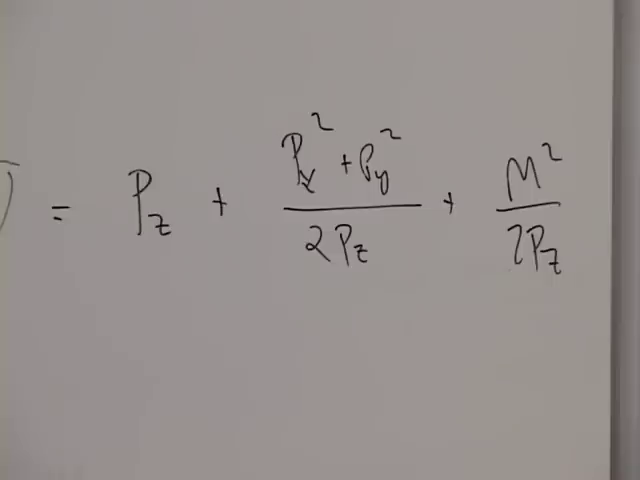
\includegraphics[width=0.76\textwidth]{lecture_02_figure_08.png}
  \caption{完成的大\(P_z\)展开，其中保留了横向动量和不变质量。}
  \lectureframe{00:47:30}
  \label{fig:l02-large-pz-board}
\end{figure}

领头项很大，但它不携带任何关于内部状态的信息。在守恒\(P_z\)的过程中，例如一个被加速的原子在不改变其总纵向动量的情况下于内部能级之间跃迁，该项会从每个能量差中消去。因此我们研究

\begin{equation}
  E-P_z=\frac{p_\perp^2+M^2}{2P_z}+O(P_z^{-3}).
  \label{eq:l02-residual-energy}
\end{equation}

分母具有物理意义。由于哈密顿量生成时间演化，这个小的剩余能量表明内部演化在实验室时间中显得缓慢。这就是时间膨胀。为了保留内部运动，引入一个重新标度的演化参数\(\tau\)，或者等价地将剩余哈密顿量乘以\(P_z\)：

\begin{equation}
  H_\perp
  \equiv
  \lim_{P_z\to\infty}P_z(E-P_z)
  =
  \frac12p_\perp^2+\frac12M^2.
  \label{eq:l02-transverse-hamiltonian}
\end{equation}

\begin{figure}[H]
  \centering
  \begin{minipage}[t]{0.48\textwidth}
    \centering
    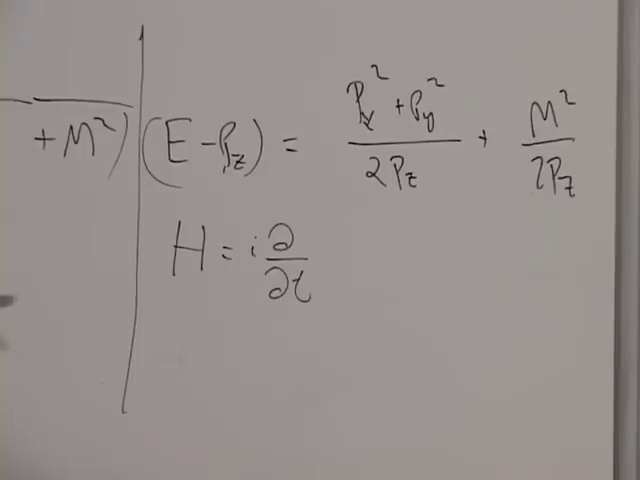
\includegraphics[width=\textwidth]{lecture_02_figure_09.png}
    \par\smallskip\footnotesize (a) \(H=i\partial_t\) 以及被减慢的内部
    演化。
  \end{minipage}\hfill
  \begin{minipage}[t]{0.48\textwidth}
    \centering
    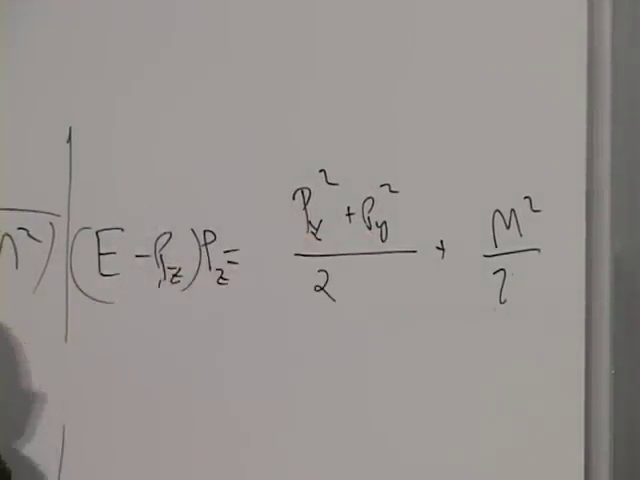
\includegraphics[width=\textwidth]{lecture_02_figure_10.png}
    \par\smallskip\footnotesize (b) 时间重标度之后的有限横向哈密顿量。
  \end{minipage}
  \caption{从时间膨胀的剩余能量到有限的
  二维哈密顿量。}
  \lectureframe{00:49:20 and 00:52:40}
  \label{fig:l02-lightfront-board}
\end{figure}

这正是一个单位质量粒子在二维中运动的哈密顿量形式：动能\(p_\perp^2/2\)加上内部能量\(M^2/2\)。不寻常的特征在于平方。在这一描述中，扮演静止能量或束缚能量角色的量正比于不变质量的平方。\editorialnote{采用传统的光前变量\(P^\pm=(E\pm P_z)/\sqrt2\)时，精确的质壳关系为\(2P^+P^-=p_\perp^2+M^2\)。方程\eqref{eq:l02-transverse-hamiltonian}是本讲中同一不变关系的大\(P_z\)归一化形式。}

\begin{classroomqa}
\audiencequestion{复合系统各个组成部分的纵向动量到哪里去了？\lecturetimestamp{00:51:30}}
\lecturerresponse{对于一般的复合客体，必须保留其组分所携带的总\(P_z\)的分数。上面的公式使用了总质心动量。弦理论之所以特殊，是因为其约束从横向自由度决定了相对纵向运动，因此不需要添加独立的纵向振子。}
\end{classroomqa}

\section{离散开弦}

被加速的弦现在明确地只在横向平面中运动。将其两个坐标标记为\(X\)和\(Y\)，并首先用\(N\)个质点由\(N-1\)根弹簧连接来近似它。如果\(\mu\)是每个质点的类比质量，\(k\)是最近邻弹簧常数，则能量为

\begin{equation}
  E_N
  =
  \sum_i
  \left[
    \frac{\mu}{2}
    \left(\dot X_i^2+\dot Y_i^2\right)
    +
    \frac{k}{2}
    \left((\Delta X_i)^2+(\Delta Y_i)^2\right)
  \right].
  \label{eq:l02-discrete-energy}
\end{equation}

每个\(X\)项都有一个相同的\(Y\)项，因为横向平面有两个方向。指标\(i\)标记链上的一个点；它不是空间坐标。

\begin{figure}[H]
  \centering
  \begin{minipage}[t]{0.48\textwidth}
    \centering
    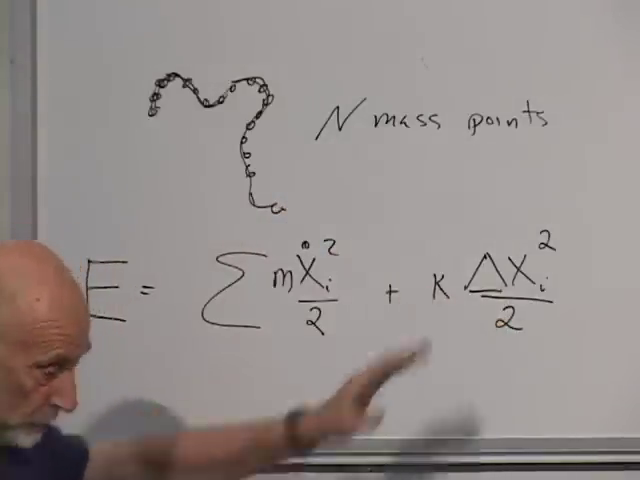
\includegraphics[width=\textwidth]{lecture_02_figure_11.png}
    \par\smallskip\footnotesize (a) 珠链及其离散能量。
  \end{minipage}\hfill
  \begin{minipage}[t]{0.48\textwidth}
    \centering
    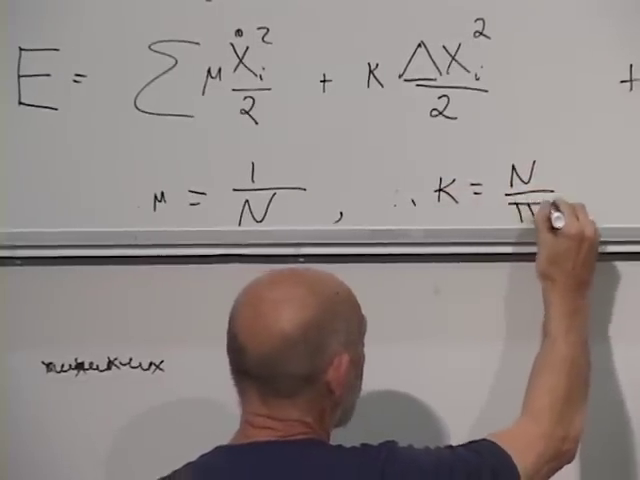
\includegraphics[width=\textwidth]{lecture_02_figure_12.png}
    \par\smallskip\footnotesize (b) \(\mu\)和\(k\)的大\(N\)标度行为。
  \end{minipage}
  \caption{取连续极限之前的正则化开弦。}
  \lectureframe{00:57:42 and 01:02:40}
  \label{fig:l02-chain-board}
\end{figure}

\begin{figure}[H]
  \centering
  \begin{adjustbox}{max width=\linewidth}
  \begin{tikzpicture}[>=Latex,thick]
    \foreach \i in {0,...,8} {
      \coordinate (p\i) at ({1.05*\i},{0.30*sin(55*\i)});
      \filldraw[white] (p\i) circle (0.10);
      \draw (p\i) circle (0.10);
    }
    \foreach \i in {0,...,7} {
      \pgfmathtruncatemacro{\j}{\i+1}
      \draw[decorate,decoration={zigzag,segment length=4pt,amplitude=2pt}]
        (p\i) -- (p\j);
    }
    \node[above=0.35cm of p0] {\(i=0\)};
    \node[above=0.35cm of p8] {\(i=N-1\)};
    \draw[<->] (0,-1.15) -- (8.4,-1.15)
      node[midway,below] {\(0\leq\sigma\leq\pi\)};
    \node at (4.2,1.25)
      {\(\mu=1/N,\quad k=N/\pi^2,\quad\Delta\sigma=\pi/N\)};
  \end{tikzpicture}
  \end{adjustbox}
  \caption{一幅清晰的正则化图像。随着链被细化，质点变得更轻，而微观弹簧变得更硬。}
  \label{fig:l02-chain-redraw}
\end{figure}

参数\(\sigma\)标记沿链的位置。选择\(0\leq\sigma\leq\pi\)是一种约定，而不是物理长度测量。它提醒我们弦有两个端点。稍后闭弦将在\(0\leq\sigma<2\pi\)上周期性地标记。

连续极限必须保持集体力学量有限。固定的珠质量会使总类比质量发散，因此选择

\begin{equation}
  \mu=\frac{1}{N}.
  \label{eq:l02-mu-scaling}
\end{equation}

于是\(N\mu=1\)。这不是相对论静止质量\(M\)；它是横向类比模型中的惯性系数。

串联的弹簧随着数目增加而变软。为了使整条链保持有限的劲度，每根微观弹簧必须变得更硬：

\begin{equation}
  k=\frac{N}{\pi^2}
  =\frac{1}{\pi\,\Delta\sigma}.
  \label{eq:l02-k-scaling}
\end{equation}

只有\(k\propto N\)是本质的。因子\(\pi^2\)是为了从连续公式中消除多余的\(\pi\)因子而选择的归一化。

\begin{classroomqa}
\audiencequestion{\(\mu\)是每个弦点的物理静止质量吗？\lecturetimestamp{01:10:34}}
\lecturerresponse{不是。它是横向链中出现的非相对论类比质量。把它称为\(M\)会与整个相对论弦状态的不变静止质量相混淆。它目前唯一的作用是产生正确的连续惯性。}
\end{classroomqa}

\section{连续波系统}

应用开头准备好的规则。由于\(1/N=\Delta\sigma/\pi\)，

\begin{align}
  \sum_i\frac{\mu}{2}\dot X_i^2
  &=
  \frac{1}{2\pi}
  \sum_i\dot X_i^2\,\Delta\sigma
  \longrightarrow
  \frac{1}{2\pi}
  \int_0^\pi
  \left(\partial_\tau X\right)^2d\sigma ,
  \label{eq:l02-kinetic-limit}\\
  \sum_i\frac{k}{2}(\Delta X_i)^2
  &\longrightarrow
  \frac{1}{2\pi}
  \int_0^\pi
  \left(\partial_\sigma X\right)^2d\sigma .
  \label{eq:l02-potential-limit}
\end{align}

对于第二行，使用\(\Delta X_i=\partial_\sigma X\,\Delta\sigma\)以及\(k=1/(\pi\Delta\sigma)\)。同样的计算适用于\(Y\)。

\begin{figure}[H]
  \centering
  \begin{minipage}[t]{0.48\textwidth}
    \centering
    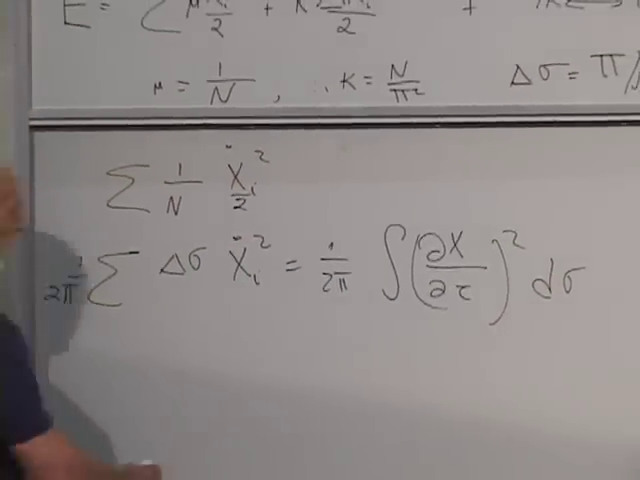
\includegraphics[width=\textwidth]{lecture_02_figure_13.png}
    \par\smallskip\footnotesize (a) 求和化为积分以及
    差分化为导数的替换。
  \end{minipage}\hfill
  \begin{minipage}[t]{0.48\textwidth}
    \centering
    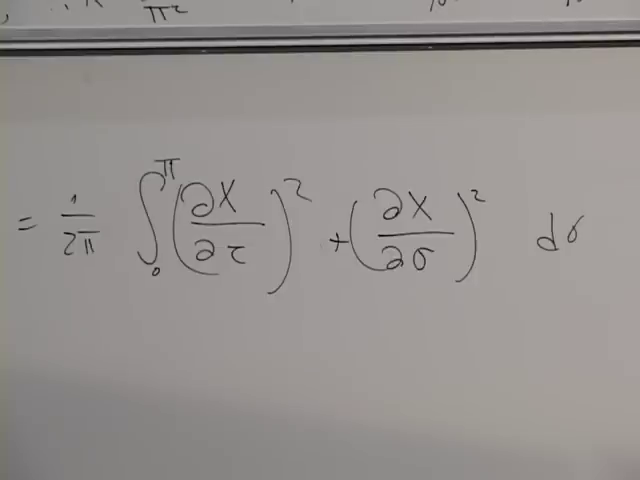
\includegraphics[width=\textwidth]{lecture_02_figure_14.png}
    \par\smallskip\footnotesize (b) 完成后的连续极限能量。
  \end{minipage}
  \caption{离散链在 \(\sigma\) 区间上变为场。}
  \lectureframe{01:05:40 and 01:07:00}
  \label{fig:l02-continuum-board}
\end{figure}

由此得到的能量和拉格朗日量为

\begin{align}
  E
  &=
  \frac{1}{2\pi}
  \int_0^\pi d\sigma\,
  \left[
    (\partial_\tau X)^2+(\partial_\tau Y)^2\right.\notag\\[-0.25em]
  &\hspace{6.5em}\left.
    +(\partial_\sigma X)^2+(\partial_\sigma Y)^2
  \right],
  \label{eq:l02-continuum-energy}\\
  L
  &=
  \frac{1}{2\pi}
  \int_0^\pi d\sigma\,
  \left[
    (\partial_\tau X)^2+(\partial_\tau Y)^2\right.\notag\\[-0.25em]
  &\hspace{6.5em}\left.
    -(\partial_\sigma X)^2-(\partial_\sigma Y)^2
  \right].
  \label{eq:l02-continuum-lagrangian}
\end{align}

\begin{figure}[H]
  \centering
  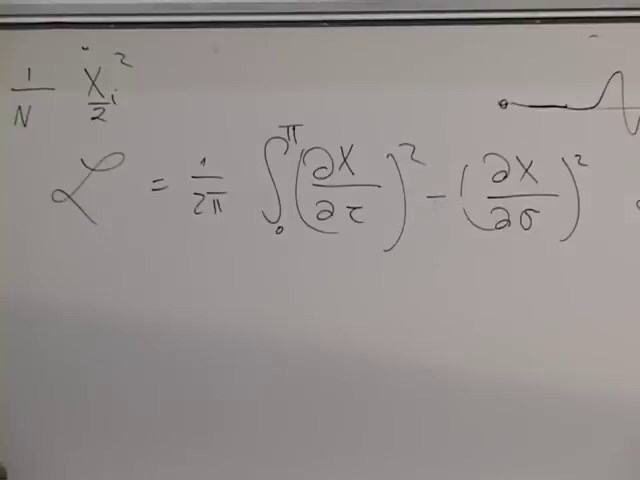
\includegraphics[width=0.78\textwidth]{lecture_02_figure_15.png}
  \caption{连续极限下的拉格朗日量，其动能项与拉伸项
  带有相反的符号。}
  \lectureframe{01:08:48}
  \label{fig:l02-lagrangian-board}
\end{figure}

如果我们把 \(\sigma\) 重新命名为一个普通空间坐标，把 \(X\) 重新命名为
一个场 \(\phi\)，那么这些就是一个一维波场的能量和拉格朗日量。对 \eqref{eq:l02-continuum-lagrangian} 作变分得到

\begin{equation}
  \left(\partial_\tau^2-\partial_\sigma^2\right)X=0,
  \qquad
  \left(\partial_\tau^2-\partial_\sigma^2\right)Y=0.
  \label{eq:l02-wave-equation}
\end{equation}

眼前的论证并不要求我们直接求解这些方程。有用的图像仅仅是：波沿弦向左和向右传播，并在端点处反射。Dirichlet 反射使位移改变符号；Neumann 反射则保持其符号不变。

\begin{classroomqa}
\audiencequestion{时间变量 \(\tau\) 究竟是什么？\lecturetimestamp{01:08:54}}
\lecturerresponse{它是在大 \(P_z\) 描述中用来追踪内部运动的重新标度时间。随系统一起作洛伦兹加速的时钟相对于实验室时间走得慢；\(\tau\) 消除了这种时间膨胀，使内部振荡保持有限的频率。对于这一横向力学而言，它可以简单地被当作时间来对待。\editorialnote{讲义中非正式地把 \(\tau\) 称为固有时。对于一根延展的弦，精确的光前演化参数是一个规范固定的重新标度时间，而不是每个点所共有的单一不变固有时。原本想要表达的时间膨胀论证并未改变。}}
\end{classroomqa}

当质心在横向平面内静止时，\eqref{eq:l02-continuum-energy} 的内部部分在
\eqref{eq:l02-transverse-hamiltonian} 的归一化下正比于 \(M^2\)。这就是为什么量子化这个表面上普通的波动系统会揭示出相对论性质量谱。

\begin{classroomqa}
\audiencequestion{\(P_z(E-P_z)\) 有
名称吗？\lecturetimestamp{01:11:00}}
\lecturerresponse{它通常被称为光锥能量或光前能量。
光前更好地描述了用作演化曲面的零平面；
传统术语对计算并不重要。}
\end{classroomqa}

\begin{classroomqa}
\audiencequestion{锥这个词是指通常的时空光锥吗，这个术语是 Dirac 引入的吗？\lecturetimestamp{01:11:17}}
\lecturerresponse{零坐标构造可以用
45 度轴来画出，但这里的演化曲面是一个光前，而不是完整的膨胀锥。Dirac 发展了相对论动力学的相关形式；历史命名问题仍悬而未决，且不影响方程。}
\end{classroomqa}

\section{为什么自由端点对应 Neumann}

我们现在可以推导而不是假设端点条件。牛顿定律是合法的，因为加速后的横向力学恰好具有非相对论形式。内部质点受到两侧弹簧的拉拽。最后一个点只受到将它与其相邻点连接起来的弹簧的拉拽。

\begin{classroomqa}
\audiencequestion{为什么在讨论相对论性弦时我们可以使用牛顿定律？\lecturetimestamp{01:14:52}}
\lecturerresponse{我们并不是把牛顿力学应用于完整的未加速时空运动。我们把它应用于无限动量描述中的横向变量，其哈密顿量恰好具有非相对论形式。}
\end{classroomqa}

在右端点处，胡克定律给出（不计取向）

\begin{equation}
  F_{\mathrm{end}}
  =
  -k\,\Delta X
  =
  -\frac{1}{\pi\Delta\sigma}
   \left(\partial_\sigma X\,\Delta\sigma\right)
  =
  -\frac{1}{\pi}\partial_\sigma X .
  \label{eq:l02-endpoint-force}
\end{equation}

\begin{figure}[H]
  \centering
  \begin{minipage}[t]{0.48\textwidth}
    \centering
    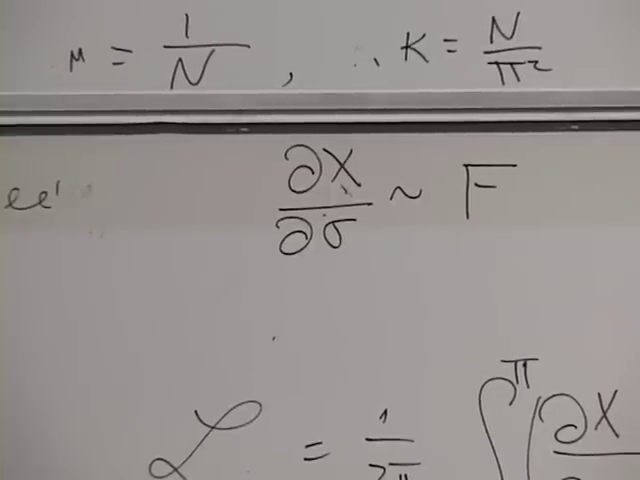
\includegraphics[width=\textwidth]{lecture_02_figure_16.png}
    \par\smallskip\footnotesize (a) 端点力正比于局部
    斜率。
  \end{minipage}\hfill
  \begin{minipage}[t]{0.48\textwidth}
    \centering
    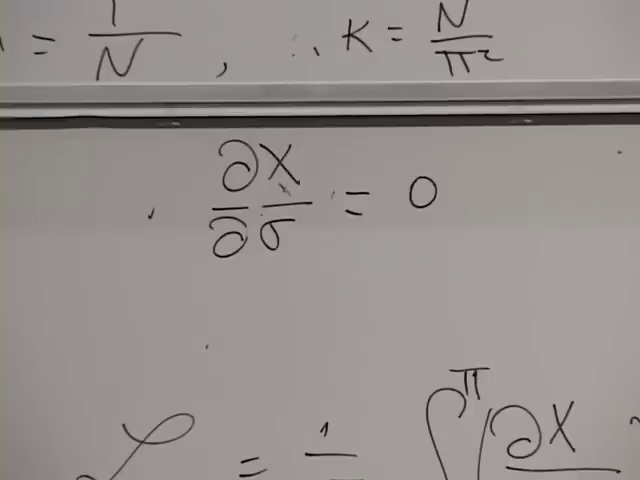
\includegraphics[width=\textwidth]{lecture_02_figure_17.png}
    \par\smallskip\footnotesize (b) 有限加速度条件。
  \end{minipage}
  \caption{自由端边界条件的牛顿定律推导。}
  \lectureframe{01:18:20 and 01:20:10}
  \label{fig:l02-neumann-board}
\end{figure}

最后一个点的牛顿方程为

\begin{equation}
  \mu\,\partial_\tau^2X=F_{\mathrm{end}},
  \qquad
  \mu=\frac1N=\frac{\Delta\sigma}{\pi}.
  \label{eq:l02-endpoint-newton}
\end{equation}

结合 \eqref{eq:l02-endpoint-force} 与
\eqref{eq:l02-endpoint-newton}，

\begin{equation}
  \partial_\sigma X
  =
  -\Delta\sigma\,\partial_\tau^2X
  \quad\text{at the right endpoint},
  \label{eq:l02-endpoint-scaling}
\end{equation}

在左端点处力的符号相反。如果
\(\partial_\sigma X\) 在
\(\Delta\sigma\to0\) 时趋于一个非零常数，则端点加速度将像 \(N\) 那样发散。
因此，一个具有有限加速度的合理连续极限要求

\begin{equation}
  \left.\partial_\sigma X\right|_{0,\pi}=0,
  \qquad
  \left.\partial_\sigma Y\right|_{0,\pi}=0.
  \label{eq:l02-open-neumann}
\end{equation}

\begin{figure}[H]
  \centering
  \begin{adjustbox}{max width=\linewidth}
  \begin{tikzpicture}[>=Latex,thick,scale=1.0]
    \coordinate (a) at (0,0);
    \coordinate (b) at (4.5,0.75);
    \filldraw[white] (a) circle (0.12);
    \draw (a) circle (0.12);
    \filldraw[white] (b) circle (0.12);
    \draw (b) circle (0.12);
    \draw[decorate,decoration={zigzag,segment length=6pt,amplitude=3pt}]
      (a) -- (b);
    \draw[dashed] (a) -- (0,-1.2);
    \draw[dashed] (b) -- (4.5,-1.2);
    \draw[<->] (4.85,0) -- (4.85,0.75)
      node[midway,right] {\(\Delta X\)};
    \draw[->,red!70!black] (b) -- (5.75,0.95)
      node[right] {\(F_{\rm end}=-k\Delta X\)};
    \node[below] at (0,-1.2) {\(N-1\)};
    \node[below] at (4.5,-1.2) {\(N\)};
    \node at (2.5,-2.0)
      {\(\mu\ddot X=-k\Delta X
      \ \Longrightarrow\
      \partial_\sigma X=-\Delta\sigma\,\ddot X\to0\)};
  \end{tikzpicture}
  \end{adjustbox}
  \caption{在正规化极限下最后一个点的质量趋于零。只有当端点斜率消失时，
  才可能有有限的加速度。}
  \label{fig:l02-neumann-redraw}
\end{figure}

在两端以及在两个横向方向上作同样的论证，就得到自由开弦的 Neumann 边界条件。

\section{开弦的简正模}

现在我们已经有了一个完整的经典系统：一个拉格朗日量及其边界条件。经过傅里叶分析之后，量子化就变得简单了。由于端点是诺伊曼端点，

\begin{align}
  X(\sigma,\tau)
  &=
  \sum_{n=0}^{\infty}X_n(\tau)\cos(n\sigma),
  \label{eq:l02-X-expansion}\\
  Y(\sigma,\tau)
  &=
  \sum_{n=0}^{\infty}Y_n(\tau)\cos(n\sigma).
  \label{eq:l02-Y-expansion}
\end{align}

余弦项包含了全部\(\sigma\)依赖。系数包含了全部时间依赖；弦之所以振动，是因为\(X_n(\tau)\)和\(Y_n(\tau)\)在变化。

\begin{figure}[H]
  \centering
  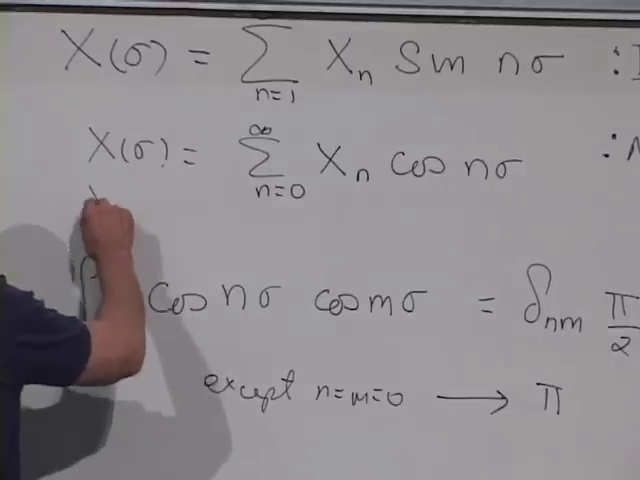
\includegraphics[width=0.78\textwidth]{lecture_02_figure_18.png}
  \caption{诺伊曼模展开式，与将把双重求和消去的正交性规则并列展示。}
  \lectureframe{01:21:45}
  \label{fig:l02-mode-expansion-board}
\end{figure}

\subsection{动能项与零模}

对时间求导给出

\begin{equation}
  \partial_\tau X
  =
  \sum_{n=0}^{\infty}\dot X_n(\tau)\cos(n\sigma).
  \label{eq:l02-time-mode}
\end{equation}

平方之后产生一个关于\(n\)和\(m\)的双重求和，但\eqref{eq:l02-cos-orthogonality}会消去每一个满足\(n\neq m\)的项。将常数模单独处理，

\begin{equation}
  \frac{1}{2\pi}\int_0^\pi
  (\partial_\tau X)^2\,d\sigma
  =
  \frac12\dot X_0^{\,2}
  +
  \frac14\sum_{n=1}^{\infty}\dot X_n^{\,2}.
  \label{eq:l02-mode-kinetic}
\end{equation}

\begin{figure}[H]
  \centering
  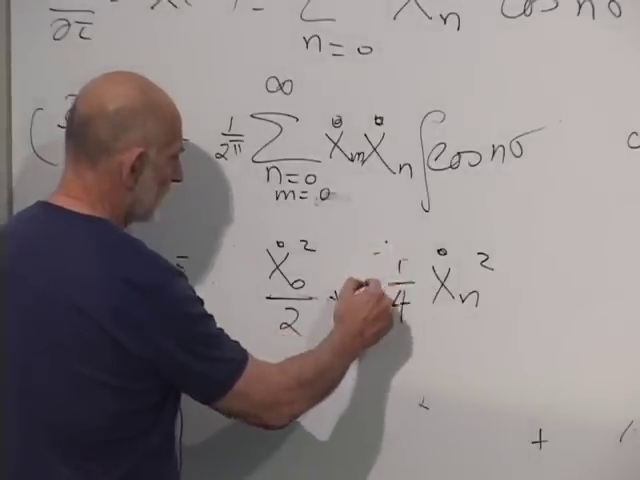
\includegraphics[width=0.76\textwidth]{lecture_02_figure_19.png}
  \caption{正交性积分将动能双重求和化为零模加上一个对角求和。}
  \lectureframe{01:29:10}
  \label{fig:l02-mode-kinetic-board}
\end{figure}

常数系数就是平均位置，

\begin{equation}
  X_0(\tau)=\frac1\pi\int_0^\pi X(\sigma,\tau)\,d\sigma ,
  \label{eq:l02-center-of-mass}
\end{equation}

对\(Y_0\)也类似。在均匀的模拟质量密度下，这些就是质心坐标。它们具有动能但没有回复力：整条弦可以在横向平面内自由运动。

\subsection{拉伸项与振子频率}

对空间求导给出

\begin{equation}
  \partial_\sigma X
  =
  -\sum_{n=1}^{\infty}nX_n(\tau)\sin(n\sigma).
  \label{eq:l02-spatial-mode}
\end{equation}

零模消失了，因为均匀平移不会拉伸弦。利用正弦正交性，

\begin{equation}
  \frac{1}{2\pi}\int_0^\pi
  (\partial_\sigma X)^2\,d\sigma
  =
  \frac14\sum_{n=1}^{\infty}n^2X_n^{\,2}.
  \label{eq:l02-mode-potential}
\end{equation}

\begin{figure}[H]
  \centering
  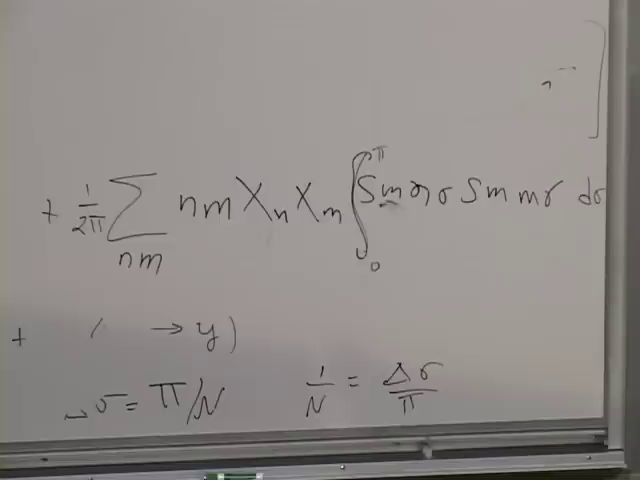
\includegraphics[width=0.76\textwidth]{lecture_02_figure_20.png}
  \caption{对余弦级数求导产生正弦双重求和；正交性再次强制\(n=m\)。}
  \lectureframe{01:31:40}
  \label{fig:l02-mode-potential-board}
\end{figure}

因此\(X\)部分的拉格朗日量为

\begin{equation}
  L_X
  =
  \frac12\dot X_0^{\,2}
  +
  \frac14\sum_{n=1}^{\infty}
  \left(
    \dot X_n^{\,2}-n^2X_n^{\,2}
  \right),
  \label{eq:l02-X-lagrangian}
\end{equation}

对\(Y\)有完全相同的表达式。相应的能量在\(n^2X_n^2\)前面有一个正号。每一个非零模都是一个独立的谐振子，与\eqref{eq:l02-oscillator-lagrangian}比较可得

\begin{equation}
  \omega_n=n,
  \qquad n=1,2,3,\ldots .
  \label{eq:l02-mode-frequency}
\end{equation}

\begin{figure}[H]
  \centering
  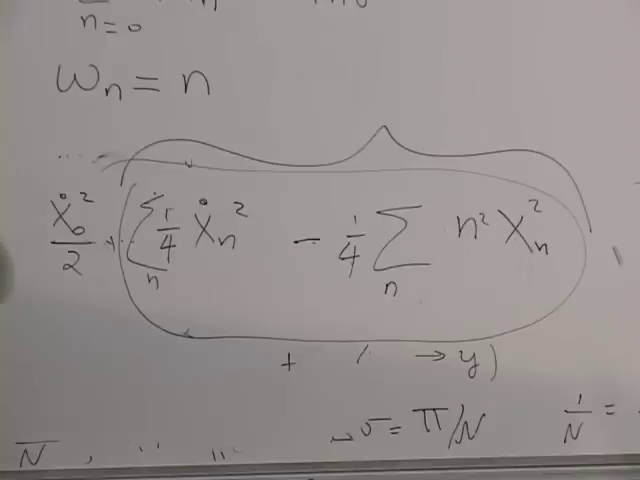
\includegraphics[width=0.80\textwidth]{lecture_02_figure_21.png}
  \caption{解耦的振子拉格朗日量以及结论\(\omega_n=n\)，下面还给出了完全相同的\(Y\)塔。}
  \lectureframe{01:35:50}
  \label{fig:l02-oscillator-modes-board}
\end{figure}

简正模就是弦的各个谐波。第一个缓慢弯曲，第二个频率是它的两倍，第三个是三倍，依此类推。正交性正是自由理论中防止一个谐波与另一个谐波耦合的原因。

\begin{classroomqa}
\audiencequestion{\(n=0\)振子怎么样了？\lecturetimestamp{01:34:49}}
\lecturerresponse{它的频率为零，因为它根本不是一个内部振子。它平移的是质心。没有任何弹簧会把整条弦恢复到某个偏好的横向位置，所以零模是一个自由粒子坐标。}
\end{classroomqa}

去掉质心动能项后，剩下的就是内能

\begin{equation}
  E_{\mathrm{int}}
  =
  \frac14
  \sum_{n=1}^{\infty}
  \left[
    \dot X_n^{\,2}+n^2X_n^{\,2}
    +\dot Y_n^{\,2}+n^2Y_n^{\,2}
  \right].
  \label{eq:l02-internal-energy}
\end{equation}

在光前归一化中，这正比于弦态的不变质量平方。这样我们就将相对论性质量问题转化成了两个可数振子塔的量子力学。

\section{量子化能级与粒子行为}

设\(a_n^\dagger\)在频率为\(n\)的\(X\)振子中产生一个量子，而\(b_n^\dagger\)对\(Y\)做同样的事。本讲推迟了系统的算符处理，但这种记号使能级计数变得透明。相对于基态偏移，

\begin{equation}
  \begin{aligned}
    \Delta E_{\mathrm{int}}
    &=\sum_{n=1}^{\infty}n\left(Q_n^X+Q_n^Y\right),\\
    Q_n^X,Q_n^Y&\in\{0,1,2,\ldots\}.
  \end{aligned}
  \label{eq:l02-quantized-energy}
\end{equation}

其中\(\hbar=1\)。整数\(n\)标记哪个振子被激发；\(Q_n\)计算它占据了多少个量子。\editorialnote{每个振子还贡献一份零点能。这个无穷求和需要正规化，并提供了弦质量公式的截距。本讲在此有意不指定基态偏移，只计激发能级。}

振子真空\(\ket{0}\)并不是空无一物的时空。它是一条没有内部振子被激发的开弦。它具有能量、动量，并在弦谱中占有确定的位置。

在第一能级上有两个态，

\begin{equation}
  a_1^\dagger\ket{0},
  \qquad
  b_1^\dagger\ket{0},
  \label{eq:l02-level-one}
\end{equation}

对应于沿\(X\)或\(Y\)极化的最低谐波。线性组合描述任意横向极化。

在第二能级上有五个态：

\begin{equation}
  (a_1^\dagger)^2\ket{0},
  \quad
  a_1^\dagger b_1^\dagger\ket{0},
  \quad
  (b_1^\dagger)^2\ket{0},
  \quad
  a_2^\dagger\ket{0},
  \quad
  b_2^\dagger\ket{0}.
  \label{eq:l02-level-two}
\end{equation}

三个使用第一谐波的两个量子；两个使用第二谐波的一个量子。两种构造都耗费两个单位。

\begin{figure}[H]
  \centering
  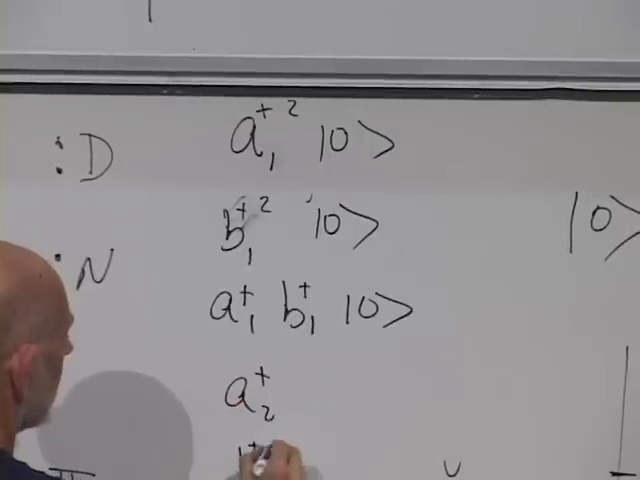
\includegraphics[width=0.76\textwidth]{lecture_02_figure_22.png}
  \caption{在听众质疑之后重新清点五个第二能级态：两个双激发、一个混合激发，以及两个第二谐波激发。}
  \lectureframe{01:44:00}
  \label{fig:l02-levels-board}
\end{figure}

\begin{figure}[H]
  \centering
  \begin{adjustbox}{max width=\linewidth}
  \begin{tikzpicture}[>=Latex,thick]
    \draw[->] (0,0) -- (0,5.1) node[above] {\(\Delta E_{\rm int}\)};
    \draw[blue!70!black] (-0.65,0.55) -- (0.65,0.55);
    \node[right] at (0.85,0.55) {\(\ket{0}\) \quad multiplicity \(1\)};
    \draw[blue!70!black] (-0.65,2.15) -- (0.65,2.15);
    \node[right] at (0.85,2.15)
      {\(a_1^\dagger\ket{0},\ b_1^\dagger\ket{0}\)
      \quad multiplicity \(2\)};
    \draw[blue!70!black] (-0.65,3.75) -- (0.65,3.75);
    \node[right,text width=8.6cm] at (0.85,3.75)
      {\((a_1^\dagger)^2\ket{0},
      a_1^\dagger b_1^\dagger\ket{0},
      (b_1^\dagger)^2\ket{0},
      a_2^\dagger\ket{0},\ b_2^\dagger\ket{0}\)
      \quad multiplicity \(5\)};
    \node[left] at (-0.75,0.55) {\(0\)};
    \node[left] at (-0.75,2.15) {\(1\)};
    \node[left] at (-0.75,3.75) {\(2\)};
  \end{tikzpicture}
  \end{adjustbox}
  \caption{两个横向方向的开弦的前三个激发能级。}
\label{fig:l02-levels-redraw}
\end{figure}

\begin{classroomqa}
\audiencequestion{第二激发态有四个还是五个态？\lecturetimestamp{01:43:04}}
\lecturerresponse{五个。将\(X_1\)激发两次、将\(Y_1\)激发两次，以及将二者各激发一次，给出三个态。将\(X_2\)激发一次或将\(Y_2\)激发一次，又给出两个态。所提议的练习是数出接下来的两个能级。}
\end{classroomqa}

本质性的结论已经显现。相邻能级之间由有限间隙分隔，且每个能级都具有有限的重数。因此，按照将其与咖啡、气体或普通小提琴弦区分开来的谱判据，量子化弦是类粒子的。稍后我们将确定哪些态在物理上是可接受的，以及哪些病态必须被去除。

\section{为什么开弦相互作用会产生闭弦}

开弦有两个端点。它的基本相互作用使弦连接和分裂。在强子图像中，可以想象一端是夸克、另一端是反夸克；它们的湮灭使两段弦连接起来。稍后所关注的基本弦不必带有那种字面意义上的强子端点解释，但局域的连接规则仍然成立。

现在让一根开弦涨落，直到它自己的两个端点彼此接近。局域地看，一个端点无法知道另一个端点属于同一根弦而不是另一根弦。如果端点终究可以连接，那么它们就可以在这里连接，从而产生一个闭合的圈。

\begin{figure}[H]
  \centering
  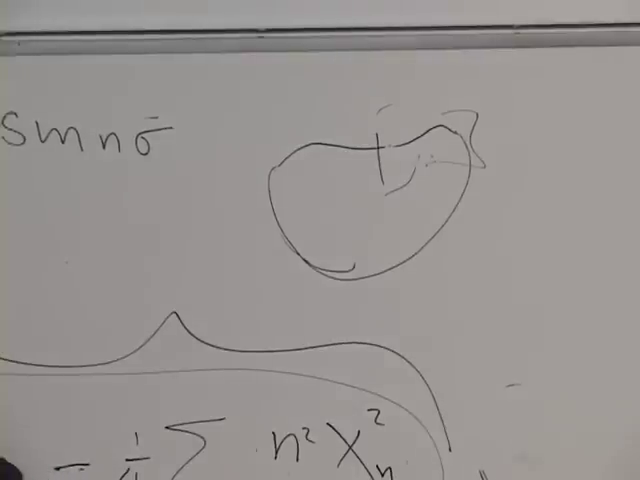
\includegraphics[width=0.70\textwidth]{lecture_02_figure_23.png}
  \caption{开弦涨落直至其两个端点相遇并形成一个闭合圈的板书示意图。}
  \lectureframe{01:47:00}
  \label{fig:l02-closed-board}
\end{figure}

\begin{figure}[H]
  \centering
  \begin{adjustbox}{max width=\linewidth}
  \begin{tikzpicture}[>=Latex,thick]
    \begin{scope}
      \draw[blue!70!black]
        (0,0) .. controls (0.8,1.2) and (1.7,-1.0) .. (2.6,0.45)
        .. controls (3.4,1.55) and (4.0,0.3) .. (4.7,0.85);
      \fill (0,0) circle (0.09);
      \fill (4.7,0.85) circle (0.09);
      \node at (2.35,-1.25) {open string fluctuation};
    \end{scope}
    \draw[->,line width=1pt] (5.25,0.3) -- (6.65,0.3)
      node[midway,above] {join};
    \begin{scope}[xshift=8.1cm]
      \draw[orange!85!black]
        (0,0) .. controls (0.3,1.5) and (2.5,1.8) .. (3.1,0.3)
        .. controls (3.5,-1.1) and (0.7,-1.5) .. (0,0);
      \node at (1.55,-1.85) {closed string};
    \end{scope}
  \end{tikzpicture}
  \end{adjustbox}
  \caption{一旦允许端点连接，开弦就可以自身闭合。}
  \label{fig:l02-closed-redraw}
\end{figure}

因此，一个理论可以包含闭弦而不包含开弦，但一个带有开弦的相互作用理论无法自洽地避免闭弦。这种不对称性就是重要的预言。谱的对应关系将在稍后展开，但目标已经显现：无质量的开弦态常常提供诸如光子之类的规范粒子，而闭弦谱则包含一个无质量的自旋二态，即引力子。一旦弦理论是相互作用的，闭弦、因而引力，就不是可有可无的装饰。

\chapter{从开弦量子到快子与引力}

\lectureoverview{我们现在对上一讲中得到的简正模进行量子化，并追问它们产生什么样的粒子态。每个横向模都是一个谐振子，但其归一化略显陌生：激发第\(n\)模会使光前能量、从而质量平方能级升高\(n\)个单位。开弦的第一激发能级的变换性质恰好与无质量矢量的两个横向极化相同。因此，相对论一致性要求基态质量平方为负。该态就是玻色弦快子，其真正意义在于真空不稳定，而不是一种实际可用的超光速粒子。最后，一旦弦发生相互作用，弦的合并与分裂使得闭弦不可避免；最低的闭弦激发将成为引力子。}

\section{隐藏在每个弦模中的谐振子}

对于一个横向坐标\(X\)，第\(n\)个非零简正模具有能量和拉格朗日量

\begin{align}
  E_n
  &=
  \frac14\dot X_n^{\,2}
  +\frac{n^2}{4}X_n^2,
  \label{eq:l03-mode-energy}\\
  L_n
  &=
  \frac14\dot X_n^{\,2}
  -\frac{n^2}{4}X_n^2.
  \label{eq:l03-mode-lagrangian}
\end{align}

\(1/4\)的因子并非错误。它们记录了将弦作用量约化为独立傅里叶模时所选择的归一化。因此，构造哈密顿量的第一步是计算正则动量，

\begin{equation}
  p_n=\frac{\partial L_n}{\partial\dot X_n}
     =\frac12\dot X_n,
  \qquad
  \dot X_n=2p_n.
  \label{eq:l03-canonical-momentum}
\end{equation}

勒让德变换给出

\begin{equation}
  H_n=p_n\dot X_n-L_n
     =p_n^2+\frac{n^2}{4}X_n^2.
  \label{eq:l03-mode-hamiltonian}
\end{equation}

\begin{figure}[H]
  \centering
  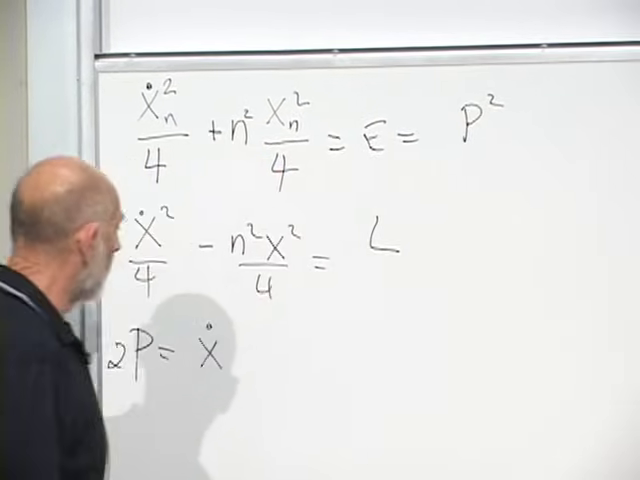
\includegraphics[width=0.82\textwidth]{lecture_03_figure_01.png}
  \caption{在从开弦继承的归一化下，模能量、拉格朗日量、正则动量与哈密顿量。}
  \lectureframe{00:05:40}
  \label{fig:l03-mode-hamiltonian-board}
\end{figure}

为了将\(H_n\)因式分解，把\(X_n\)与\(p_n\)组合为

\begin{equation}
  \frac{nX_n}{2}\pm i p_n.
\end{equation}

经典地，这两个因子会对易，但量子力学地

\begin{equation}
  [X_n,p_m]=i\delta_{nm}
  \label{eq:l03-canonical-commutator}
\end{equation}

在以\(\hbar=1\)为单位的条件下。交叉项并不会无害地相消。对于一个固定模，

\begin{align}
  \left[\frac{nX_n}{2}+ip_n,
        \frac{nX_n}{2}-ip_n\right]
  &=n,
  \label{eq:l03-unscaled-commutator}\\
  \left(\frac{nX_n}{2}-ip_n\right)
  \left(\frac{nX_n}{2}+ip_n\right)
  &=H_n-\frac n2.
  \label{eq:l03-factorized-hamiltonian}
\end{align}

\begin{figure}[H]
  \centering
  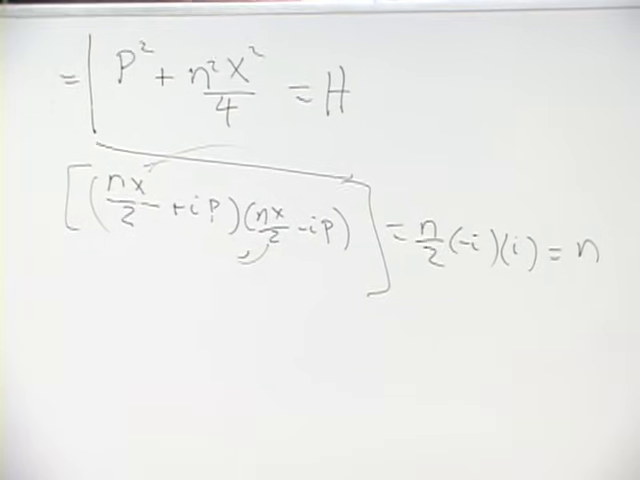
\includegraphics[width=0.82\textwidth]{lecture_03_figure_02.png}
  \caption{黑板计算中，正则对易子提供了\(n\)的因子。}
  \lectureframe{00:10:30}
  \label{fig:l03-commutator-board}
\end{figure}

\(n\)的因子告诉我们如何归一化升降算符：

\begin{align}
  a_n
  &\equiv
  \frac{\sqrt n}{2}X_n+\frac{i}{\sqrt n}p_n,
  \label{eq:l03-annihilator}\\
  a_n^\dagger
  &\equiv
  \frac{\sqrt n}{2}X_n-\frac{i}{\sqrt n}p_n.
  \label{eq:l03-creator}
\end{align}

它们满足

\begin{equation}
  [a_n,a_m^\dagger]=\delta_{nm},
  \qquad
  H_n=n\left(a_n^\dagger a_n+\frac12\right).
  \label{eq:l03-oscillator-algebra}
\end{equation}

因此，\(a_n^\dagger\)增加第\(n\)个谐振子的一个量子，但该量子携带\(n\)个单位的模能量。熟悉的谐振子间距并未丢失；其频率为\(\omega_n=n\)。

\begin{figure}[H]
  \centering
  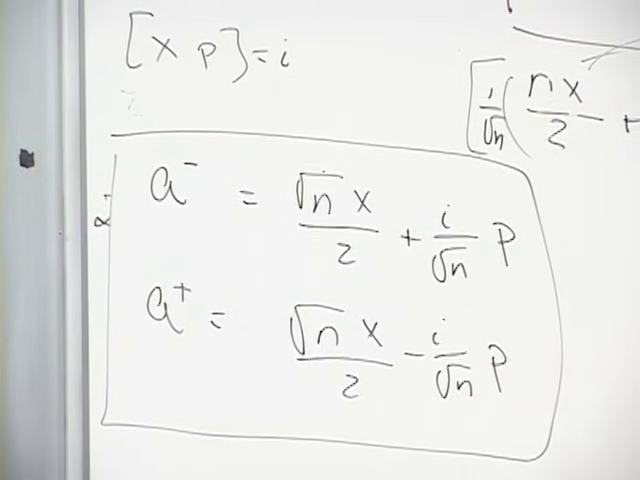
\includegraphics[width=0.82\textwidth]{lecture_03_figure_03.png}
  \caption{第\(n\)个弦谐振子的归一化湮灭算符与产生算符。}
  \lectureframe{00:12:00}
  \label{fig:l03-ladder-board}
\end{figure}

\subsection{两座横向振子塔}

在四维时空中，一根沿\(z\)轴携带极大动量的弦有两个横向坐标，\(X\)和\(Y\)。因此我们需要两座独立的振子塔。令\(a_n,a_n^\dagger\)作用于\(X\)模，\(b_n,b_n^\dagger\)作用于\(Y\)模。由\eqref{eq:l03-annihilator}--\eqref{eq:l03-creator}解出坐标，得到

\begin{equation}
  X_n=\frac{a_n+a_n^\dagger}{\sqrt n},
  \qquad
  Y_n=\frac{b_n+b_n^\dagger}{\sqrt n}.
  \label{eq:l03-mode-coordinates}
\end{equation}

\begin{figure}[H]
  \centering
  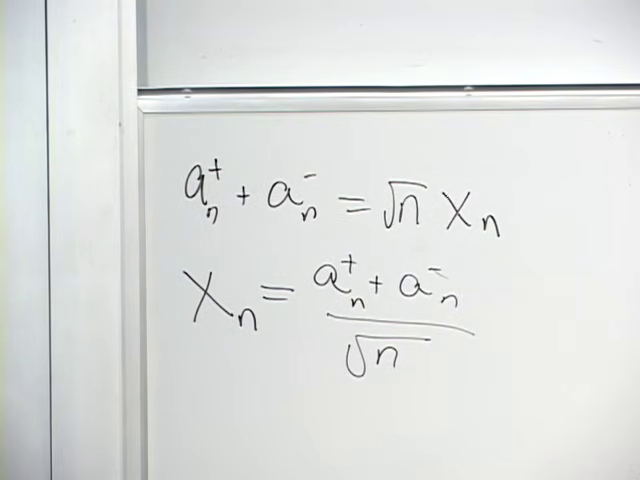
\includegraphics[width=0.78\textwidth]{lecture_03_figure_04.png}
  \caption{用产生算符与湮灭算符解出模坐标。}
  \lectureframe{00:17:05}
  \label{fig:l03-coordinate-operator-board}
\end{figure}

开弦坐标按诺伊曼模展开，

\begin{align}
  X(\sigma,\tau)
  &=X_{\rm cm}(\tau)
    +\sum_{n=1}^{\infty}X_n(\tau)\cos(n\sigma),
  \label{eq:l03-X-fourier}\\
  Y(\sigma,\tau)
  &=Y_{\rm cm}(\tau)
    +\sum_{n=1}^{\infty}Y_n(\tau)\cos(n\sigma).
  \label{eq:l03-Y-fourier}
\end{align}

出现余弦是因为端点斜率消失。代入\eqref{eq:l03-mode-coordinates}使弦本身成为一个算符：

\begin{align}
  X(\sigma,\tau)
  &=X_{\rm cm}(\tau)
    +\sum_{n=1}^{\infty}
      \frac{a_n(\tau)+a_n^\dagger(\tau)}{\sqrt n}
      \cos(n\sigma),
  \label{eq:l03-X-operator}\\
  Y(\sigma,\tau)
  &=Y_{\rm cm}(\tau)
    +\sum_{n=1}^{\infty}
      \frac{b_n(\tau)+b_n^\dagger(\tau)}{\sqrt n}
      \cos(n\sigma).
  \label{eq:l03-Y-operator}
\end{align}

\begin{figure}[H]
  \centering
  \begin{minipage}[t]{0.48\textwidth}
    \centering
    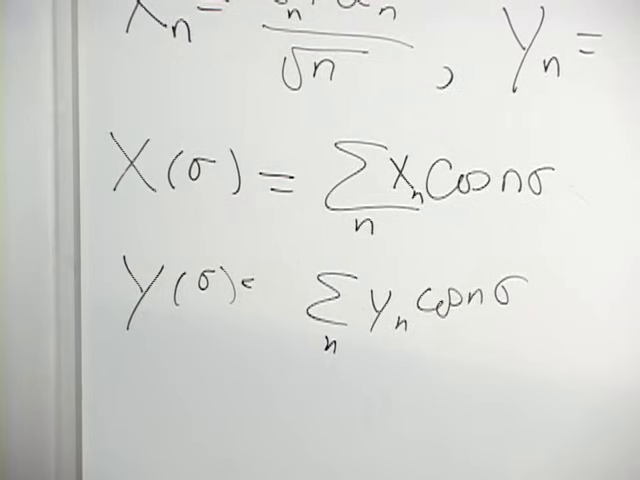
\includegraphics[width=\textwidth]{lecture_03_figure_05.png}
    \par\smallskip\footnotesize (a) 坐标模展开。
  \end{minipage}\hfill
  \begin{minipage}[t]{0.48\textwidth}
    \centering
    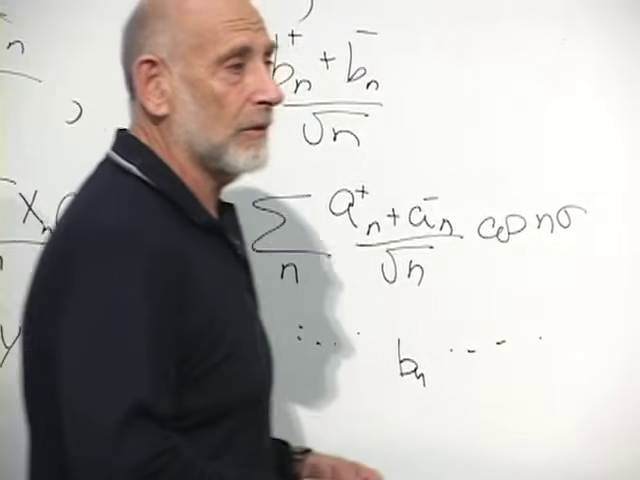
\includegraphics[width=\textwidth]{lecture_03_figure_06.png}
    \par\smallskip\footnotesize (b) 将升降算符代入弦坐标。
  \end{minipage}
  \caption{量子开弦的形状由其所有横向振子算符组装而成。}
  \lectureframe{00:20:35 and 00:21:05}
  \label{fig:l03-string-coordinate-board}
\end{figure}

\begin{classroomqa}
\audiencequestion{\(X_n\)也是\(\sigma\)的函数吗？\lecturetimestamp{00:21:48}}
\lecturerresponse{不是。对\(\sigma\)的依赖完全在\(\cos(n\sigma)\)中。系数\(X_n\)是该空间模式的时间依赖振幅，所以\(X_n=X_n(\tau)\)。}
\end{classroomqa}

\begin{classroomqa}
\audiencequestion{为什么被称为升算符和降算符的算符，其符号看起来是反的？\lecturetimestamp{00:23:13}}
\lecturerresponse{\(ip_n\)的可见符号并不是命名规则。计算其与哈密顿量的对易子。满足\([H_n,a_n^\dagger]=n a_n^\dagger\)的算符升高能量；满足\([H_n,a_n]=-n a_n\)的算符降低能量。}
\end{classroomqa}

这两座横向振子塔是一种教学性的四维图像。一致量子化的玻色弦有二十六维时空，因此它有二十四个横向振子族，而不是两个。下面的逻辑不变：第一能级态的数目必须与同一维度中无质量矢量的物理极化数目相匹配。

\section{有质量自旋与无质量螺旋度}

在给弦态指定自旋之前，我们需要一个明确的区分。一个自旋为\(J\)的有质量粒子有\(2J+1\)个自旋态，

\begin{equation}
  m_J=-J,-J+1,\ldots,J-1,J.
  \label{eq:l03-massive-spin-multiplet}
\end{equation}

例如，一个有质量的自旋为1的粒子有三种极化，一个有质量的自旋为2的粒子有五种。我们可以通过转到静止系来理解原因。在静止系中，所有空间旋转都是可用的。旋转自旋轴，再变换回去，所有\(2J+1\)个分量都属于同一个相对论性粒子。

无质量粒子没有静止系。它的不变自旋标签是螺旋度，即沿其运动方向的角动量。光子只有\(h=+1\)和\(h=-1\)；引力子只有\(h=+2\)和\(h=-2\)。标量有一个\(h=0\)态。本讲用反射对称性将两个螺旋度配对。在手性理论中，单个无质量不可约表示可能只携带一个螺旋度，因此这种配对是一个额外的对称性陈述，而不是仅由无质量性带来的结果。\editorialnote{现代小群分类允许单螺旋度的无质量表示。在熟悉的光子和引力子例子中，宇称或适当的CPT完备场内容提供了相反的螺旋度。}

\begin{figure}[H]
  \centering
  \begin{minipage}[t]{0.45\textwidth}
    \centering
    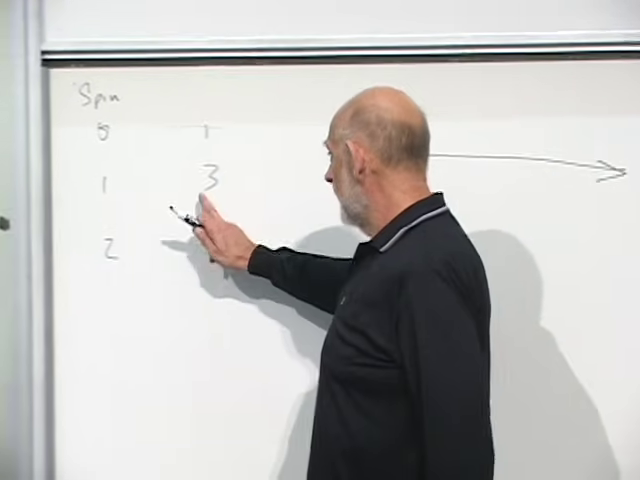
\includegraphics[width=\textwidth]{lecture_03_figure_07.png}
    \par\smallskip\footnotesize (a) 黑板上开始的自旋态计数。
  \end{minipage}\hfill
  \begin{minipage}[t]{0.5\textwidth}
    \centering
    \begin{adjustbox}{max width=\linewidth}
    \begin{tabular}{@{}ccc@{}}
      \toprule
      自旋 & 有质量态 & 无质量螺旋度 \\
      \midrule
      \(0\) & \(1\) & \(0\) \\
      \(1\) & \(3\) & \(+1,-1\) \\
      \(2\) & \(5\) & \(+2,-2\) \\
      \bottomrule
    \end{tabular}
    \end{adjustbox}
  \end{minipage}
  \caption{质量消除了静止系，也消除了中间的自旋投影。}
  \lectureframe{00:27:40}
  \label{fig:l03-spin-count}
\end{figure}

\subsection{线偏振与圆偏振光子}

取一个沿\(z\)运动的光子。它的两个横向线偏振是\(\ket{x}\)和\(\ket{y}\)。它们不是螺旋度本征态。圆偏振态是

\begin{align}
  \ket{R}
  &=\frac{1}{\sqrt2}\left(\ket{x}+i\ket{y}\right),
  \label{eq:l03-right-circular}\\
  \ket{L}
  &=\frac{1}{\sqrt2}\left(\ket{x}-i\ket{y}\right),
  \label{eq:l03-left-circular}
\end{align}

其螺旋度为\(+1\)和\(-1\)，取决于用来命名右旋和左旋的约定。线偏振光子是这两种结果的叠加。它的平均螺旋度可以为零，但螺旋度测量永远不会发现自旋为零的光子。同样，

\begin{equation}
  \frac{1}{\sqrt2}\left(\ket{x}+\ket{y}\right)
\end{equation}

就是四十五度方向的线偏振。

\begin{figure}[H]
  \centering
  \begin{minipage}[t]{0.48\textwidth}
    \centering
    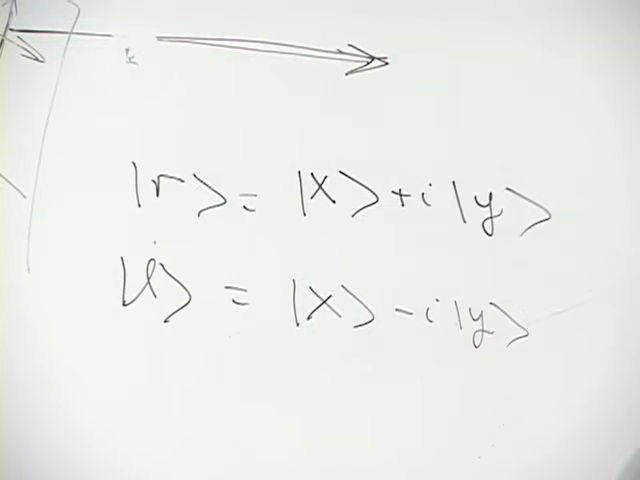
\includegraphics[width=\textwidth]{lecture_03_figure_08.png}
    \par\smallskip\footnotesize (a) 黑板上的圆偏振态。
  \end{minipage}\hfill
  \begin{minipage}[t]{0.48\textwidth}
    \centering
    \begin{adjustbox}{max width=\linewidth}
    \begin{tikzpicture}[>=Latex,scale=0.9]
      \draw[->,thick] (0,0) -- (3.4,0) node[right] {\(z\)};
      \draw[->,blue!70!black,thick] (0,0) -- (0,2.0)
        node[above] {\(x\)};
      \draw[->,orange!85!black,thick] (0,0) -- (-1.4,-1.2)
        node[below left] {\(y\)};
      \draw[red!70!black,thick,->]
        plot[domain=0:320,samples=80]
        ({1.0*cos(\x)},{0.58*sin(\x)+0.4});
      \node[red!70!black] at (1.55,1.25) {circular};
    \end{tikzpicture}
    \end{adjustbox}
  \end{minipage}
  \caption{线偏振提供横向基；圆偏振组合使螺旋度对角化。}
  \lectureframe{00:37:45}
  \label{fig:l03-polarization}
\end{figure}

\begin{classroomqa}
\audiencequestion{这是否类似于Stern--Gerlach实验中自旋态的分离？\lecturetimestamp{00:37:40}}
\lecturerresponse{量子叠加的想法是一样的，但对光子来说，直接的语言是偏振。圆偏振测量区分两个螺旋度；束流中不存在纵向的自旋为零的光子。}
\end{classroomqa}

引力子在自旋为2时重复了这一模式。为了进行自旋记账，可以示意性地写出

\begin{equation}
  \ket{+2}\sim\ket{+1}\otimes\ket{+1},
  \qquad
  \ket{-2}\sim\ket{-1}\otimes\ket{-1}.
  \label{eq:l03-graviton-helicity}
\end{equation}

这并不意味着引力子字面上由两个光子组成。它说的是两个相等的螺旋度相加得到正确的自旋为2的螺旋度。

\begin{classroomqa}
\audiencequestion{双光子类比是否推广到其他量子数？\lecturetimestamp{00:41:05}}
\lecturerresponse{不能作为组分模型。有一些强有力的公式，其中引力振幅看起来像规范理论振幅的乘积，或``平方，''但引力子仍然是它自己的粒子。这里的类比最可靠之处在于它是关于螺旋度的陈述。\editorialnote{现代Kawai--Lewellen--Tye关系和双拷贝关系在适当的理论中使振幅陈述变得精确；它们并不会把引力子变成两个光子的束缚态。}}
\end{classroomqa}

\begin{classroomqa}
\audiencequestion{光子可以具有任意动量，那么它难道不具有连续谱，而不是粒子所要求的孤立谱吗？\lecturetimestamp{00:42:17}}
\lecturerresponse{连续变量是质心动量。保持该动量固定，检查内部不变质量。粒子由孤立的质谱层来标识；改变其总动量则产生通常的连续色散关系。}
\end{classroomqa}

\section{最低的开弦能级}

现在我们可以回到弦。在大动量描述中，有限的内部光前能量正比于不变质量的平方。略去整体弦标度，将谱写成

\begin{equation}
  \begin{aligned}
    M^2
    &=m_0^2
      +\sum_{n=1}^{\infty}n
       \left(N_n^{(a)}+N_n^{(b)}\right),\\
    N_n^{(a)}&=a_n^\dagger a_n,
    \qquad
    N_n^{(b)}=b_n^\dagger b_n.
  \end{aligned}
  \label{eq:l03-open-spectrum}
\end{equation}

振子基态满足

\begin{equation}
  a_n\ket{0}=0,
  \qquad
  b_n\ket{0}=0,
  \qquad n=1,2,\ldots .
  \label{eq:l03-ground-annihilation}
\end{equation}

它并不是弦的空无缺席。它是最低激发的量子弦，其坐标仍然在涨落。设其质量平方为\(m_0^2\)，尚未确定。

\begin{figure}[H]
  \centering
  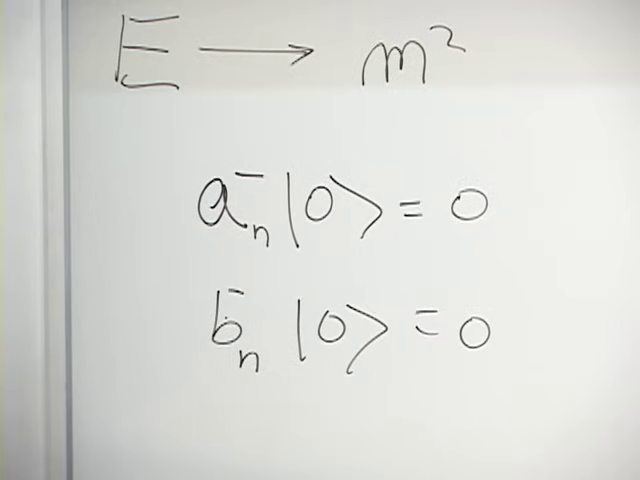
\includegraphics[width=0.78\textwidth]{lecture_03_figure_09.png}
  \caption{开弦基态以及定义它的湮灭条件。}
  \lectureframe{00:45:20}
  \label{fig:l03-ground-state-board}
\end{figure}

最廉价的激发使用\(n=1\)产生算符：

\begin{equation}
  a_1^\dagger\ket{0},
  \qquad
  b_1^\dagger\ket{0},
  \qquad
  M^2=m_0^2+1.
  \label{eq:l03-first-level}
\end{equation}

\begin{figure}[H]
  \centering
  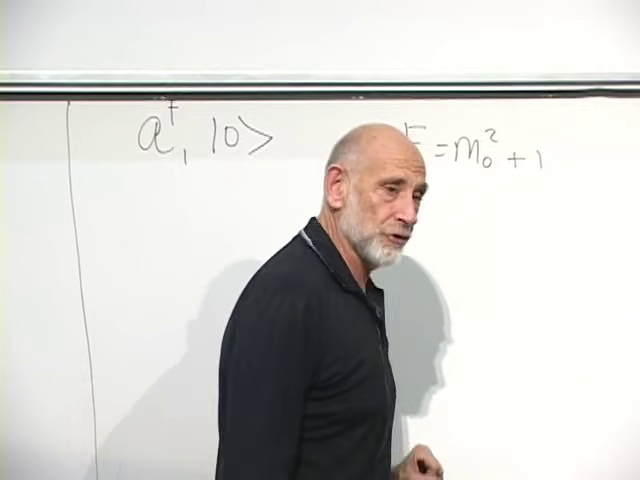
\includegraphics[width=0.78\textwidth]{lecture_03_figure_10.png}
  \caption{两个简并的第一能级态之一，黑板上写有其质量平方增量。}
  \lectureframe{00:49:25}
  \label{fig:l03-first-level-board}
\end{figure}

``一''在式{eq:l03-first-level}中不是一焦耳、一电子伏特，也不是一个普朗克质量。我们已经隐去了有量纲的弦标度。就目前而言，它指的是振子质量平方阶梯中的一步；缺失的单位将在下一讲中恢复。

这两个简并态的任何线性组合也是此能级上的一个态。特别地，

\begin{equation}
  \frac{1}{\sqrt2}
  \left(a_1^\dagger\pm i b_1^\dagger\right)\ket{0}
  \label{eq:l03-string-circular-states}
\end{equation}

是圆偏振的弦类比。在\(x\)-\(y\)平面中的旋转下，\(a_1^\dagger\)和\(b_1^\dagger\)的变换如同横向矢量的两个分量。因此\eqref{eq:l03-string-circular-states}中的组合具有螺旋度\(+1\)和\(-1\)。

\begin{figure}[H]
  \centering
  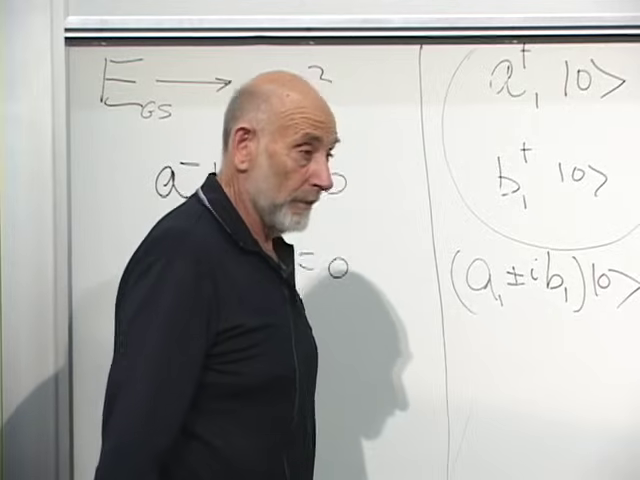
\includegraphics[width=0.82\textwidth]{lecture_03_figure_11.png}
  \caption{黑板上汇集了基态条件、两个第一能级激发及其圆组合。}
  \lectureframe{00:56:00}
  \label{fig:l03-level-structure-board}
\end{figure}

不存在可作为纵向偏振的第三个简并态。如果这两个态具有非零质量，自旋为一的相对论性粒子将需要三种偏振。恰好只有两种，该态就必须是无质量的。因此

\begin{equation}
  m_0^2+1=0,
  \qquad
  m_0^2=-1.
  \label{eq:l03-intercept-condition}
\end{equation}

第一能级是类光子的：它是一个无质量规范矢量态。它不必是电磁学中的光子；其最终的规范身份取决于弦模型。其下方的基态具有负质量平方。那就是玻色开弦快子。\editorialnote{在完整临界玻色弦中，正规序截距和洛伦兹代数与\(D=26\)相联系。本讲中两个横向方向的计算是同一态计数论证的四维投影：\(D-2\)个第一能级振子态与无质量矢量的\(D-2\)个物理偏振相匹配。}

\begin{classroomqa}
\audiencequestion{我们为什么应当关心\(m_0^2\)为负？\lecturetimestamp{00:56:35}}
\lecturerresponse{因为质量平方是二次场势关于我们称为真空的态的曲率。负曲率意味着该构型不是稳定的基态。接下来的计算将使这一陈述变得精确。}
\end{classroomqa}

\section{快子真正意味着什么}

``快子''这一名称会招致一种误导性的第一想法。从\(c=1\)的相对论色散关系出发，

\begin{equation}
  E(p)=\sqrt{p^2+m^2}.
  \label{eq:l03-relativistic-dispersion}
\end{equation}

对于波包，群速度为

\begin{equation}
  v_g=\frac{dE}{dp}.
  \label{eq:l03-group-velocity}
\end{equation}

这重现了熟悉的情形：

\begin{align}
  E_{\rm nr}(p)&=\frac{p^2}{2m},
  &v_g&=\frac{p}{m},
  \label{eq:l03-nr-group-velocity}\\
  E_\gamma(p)&=|p|,
  &|v_g|&=1,
  \label{eq:l03-photon-group-velocity}\\
  E_m(p)&=\sqrt{p^2+m^2},
  &|v_g|&=\frac{|p|}{\sqrt{p^2+m^2}}<1.
  \label{eq:l03-massive-group-velocity}
\end{align}

\begin{figure}[H]
  \centering
  \begin{minipage}[t]{0.48\textwidth}
    \centering
    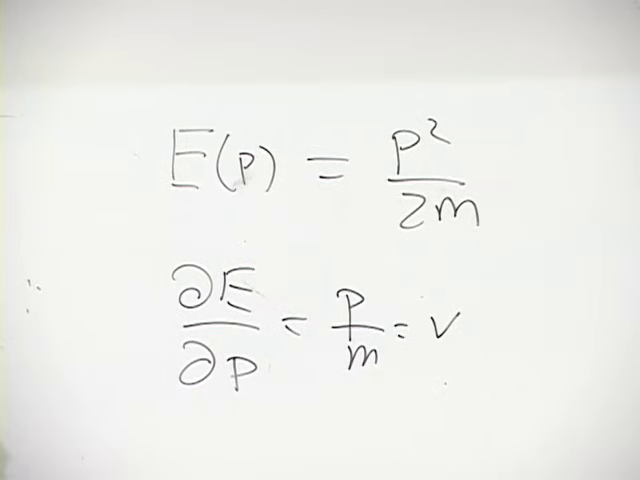
\includegraphics[width=\textwidth]{lecture_03_figure_12.png}
    \par\smallskip\footnotesize (a) 非相对论群速度。
  \end{minipage}\hfill
  \begin{minipage}[t]{0.48\textwidth}
    \centering
    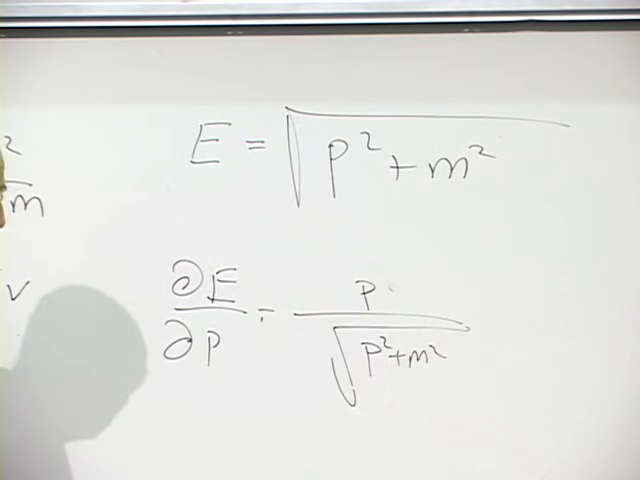
\includegraphics[width=\textwidth]{lecture_03_figure_13.png}
    \par\smallskip\footnotesize (b) 相对论色散及其
    导数。
  \end{minipage}
  \caption{从\(E(p)\)的斜率读取传播速率。}
  \lectureframe{01:01:50 and 01:03:15}
  \label{fig:l03-group-velocity-board}
\end{figure}

如果\(m^2=-\mu^2\)，形式表达式变为

\begin{equation}
  E(p)=\sqrt{p^2-\mu^2},
  \qquad
  v_g=\frac{p}{\sqrt{p^2-\mu^2}},
  \label{eq:l03-formal-tachyon-dispersion}
\end{equation}

只要平方根为实数，它就有\(|v_g|>1\)。但这不是玻色弦基态的正确物理解释。问题在低动量处就已经出现，那里频率是虚的。

\subsection{场势的负曲率}

考虑一维空间中的实标量场，

\begin{equation}
  \left(\partial_t^2-\partial_x^2+m^2\right)\phi=0.
  \label{eq:l03-klein-gordon}
\end{equation}

对于平面波\(\phi\propto e^{-i\omega t+ikx}\)，

\begin{equation}
  \omega^2=k^2+m^2.
  \label{eq:l03-kg-dispersion}
\end{equation}

\begin{figure}[H]
  \centering
  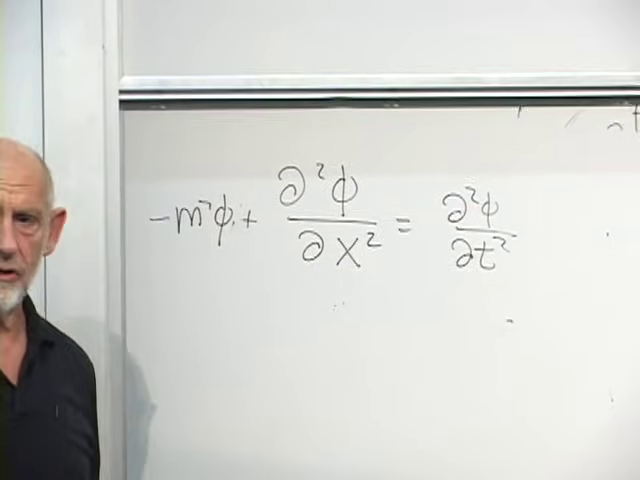
\includegraphics[width=0.82\textwidth]{lecture_03_figure_14.png}
  \caption{用于揭示负质量平方背后不稳定性的Klein--Gordon方程。}
  \lectureframe{01:06:40}
  \label{fig:l03-klein-gordon-board}
\end{figure}

守恒的二次能量为

\begin{equation}
  \mathcal E
  =\frac12\int dx\,
  \left[
    \dot\phi^{\,2}
    +(\partial_x\phi)^2
    +m^2\phi^2
  \right].
  \label{eq:l03-field-energy}
\end{equation}

\begin{figure}[H]
  \centering
  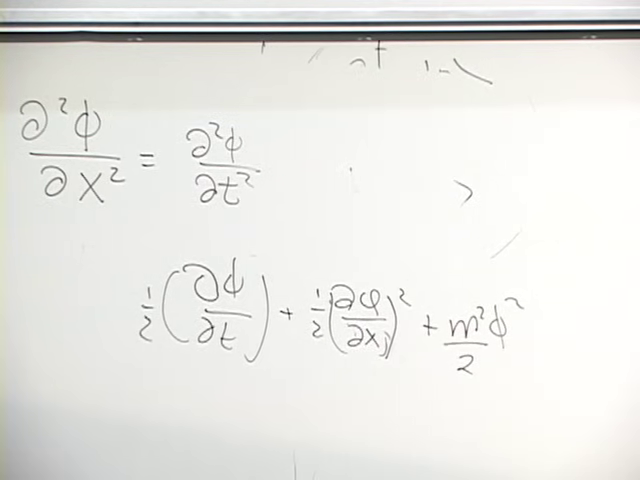
\includegraphics[width=0.82\textwidth]{lecture_03_figure_15.png}
  \caption{标量场能量，其中质量项提供势的局部曲率。}
  \lectureframe{01:08:10}
  \label{fig:l03-field-energy-board}
\end{figure}

对于\(m^2>0\)，局部势\(V(\phi)=\tfrac12m^2\phi^2\)是一个碗。构型\(\phi=0\)位于其底部。对于\(m^2=-\mu^2\)，同一点是倒置碗的顶部。方程\eqref{eq:l03-kg-dispersion}变为

\begin{equation}
  \omega^2=k^2-\mu^2.
  \label{eq:l03-tachyonic-modes}
\end{equation}

具有\(k^2<\mu^2\)的模有

\begin{equation}
  \omega=\pm i\sqrt{\mu^2-k^2},
  \qquad
  \phi_k(t)\propto
  e^{\pm\sqrt{\mu^2-k^2}\,t}.
  \label{eq:l03-growing-mode}
\end{equation}

一个分支指数增长。因此所谓的真空是不稳定的：任意小的长波扰动都会驱使场离开\(\phi=0\)。这就是谱中存在快子的含义。

\subsection{倒立摆链}

一排耦合摆使这一区别变得可见。让每个摆都竖直向上。均匀构型存在，但它平衡在势能的极大值处。轻推一个摆，它就会倒下，并拉动它的邻居。一个倒下的摆形成的前沿以由耦合固定的有限信号速度在链中传播。

\begin{figure}[H]
  \centering
  \begin{minipage}[t]{0.48\textwidth}
    \centering
    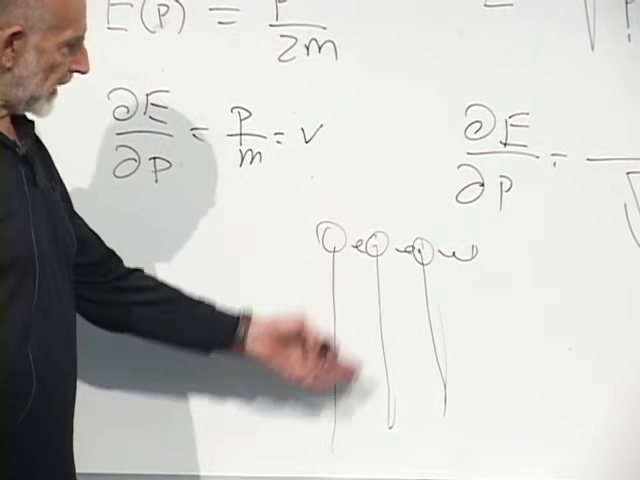
\includegraphics[width=\textwidth]{lecture_03_figure_16.png}
    \par\smallskip\footnotesize (a) 黑板上的耦合竖直摆模型。
  \end{minipage}\hfill
  \begin{minipage}[t]{0.48\textwidth}
    \centering
    \begin{adjustbox}{max width=\linewidth}
    \begin{tikzpicture}[>=Latex,scale=0.78]
      \draw[thick] (-0.3,0) -- (6.3,0);
      \foreach \x/\a in {0/0,1/0,2/8,3/28,4/55,5/72,6/78}{
        \fill (\x,0) circle (0.06);
        \draw[thick] (\x,0) -- ++({90-\a}:1.25);
        \fill[blue!65!black]
          ($(\x,0)+({90-\a}:1.25)$) circle (0.11);
      }
      \draw[red!70!black,->,thick] (1.7,-0.45) -- (4.6,-0.45)
        node[midway,below] {falling front};
    \end{tikzpicture}
    \end{adjustbox}
  \end{minipage}
  \caption{不稳定性在一个系统中以因果方式传播，即使其线性化谱包含负质量平方。}
  \lectureframe{01:10:40}
  \label{fig:l03-pendulum-instability}
\end{figure}

这一机制中没有任何东西允许受控信号超过因果前沿。快子模式诊断的是一个糟糕的展开点，而不是一个稳定的超光速信使。\editorialnote{对于局部相对论性场方程，前沿速度仍然是因果速度。实的高-\(k\)支的形式群速度并不会把不稳定真空变成超光速通信通道。}

\begin{classroomqa}
\audiencequestion{刚刚发现的无质量态就是弦理论预言的引力子吗？\lecturetimestamp{01:14:27}}
\lecturerresponse{不是。它是开弦的双极化自旋一态，因此类似规范玻色子。引力子是闭弦的自旋二激发。}
\end{classroomqa}

\begin{classroomqa}
\audiencequestion{倒置的势在数学上允许吗？系统在落下之后会在哪里结束？\lecturetimestamp{01:15:17}}
\lecturerresponse{它是一个完全合法的局部近似，但仅凭它自身没有基态，因为能量无下界。更完整的势可能再次向上弯折并拥有一个更低的极小值。系统随后会滚向或凝聚到那个稳定构型。}
\end{classroomqa}

普通的玻色弦恰好具有这一缺陷。它的更高振子态仍然是谱的一部分，但它们是不稳定背景的激发。自洽的超弦理论在其稳定扇区中移除开弦快子，同时保留无质量和有质量的弦激发。

\begin{classroomqa}
\audiencequestion{开弦态的其他性质是否也像它的两个极化那样与光子相符？\lecturetimestamp{01:17:07}}
\lecturerresponse{该态的行为如同无质量规范玻色子。它的详细电荷分配、辐射规则和身份取决于弦模型，因此应当称它类光子，而不是立即把它等同于电磁作用。那些相互作用性质将在后面展开。}
\end{classroomqa}

\section{弦如何相互作用}

自由谱只是理论的一半。弦也会结合和分裂。首先记住，一个激发的自由弦可以携带角动量是有用的。一根直的旋转弦绕其质心转动，它的能量和角动量沿着熟悉的弦轨迹一起上升。

\begin{figure}[H]
  \centering
  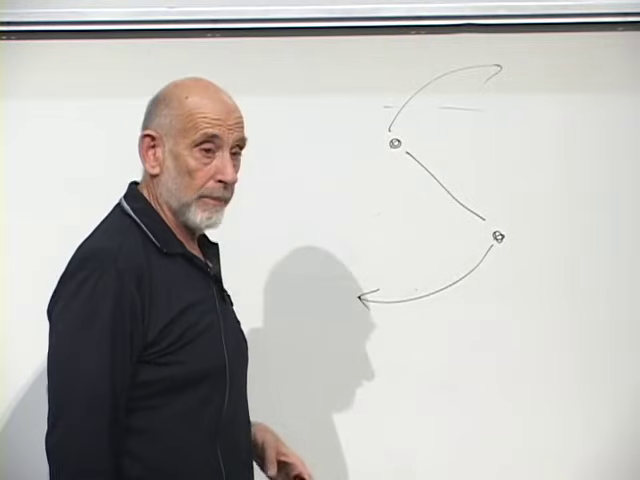
\includegraphics[width=0.72\textwidth]{lecture_03_figure_17.png}
  \caption{一根绕其质心点旋转的开弦的示意图。}
  \lectureframe{01:19:30}
  \label{fig:l03-rotating-string-board}
\end{figure}

\begin{classroomqa}
\audiencequestion{一根自由弦能绕一个固定端点翻转旋转吗？\lecturetimestamp{01:20:02}}
\lecturerresponse{没有锚点就不行。一个自由的孤立系统绕其质心旋转。如果一个端点附着在另一个物体或一个膜上，那么组合系统可以绕一个不同的中心旋转，正如电子和原子核绕它们的共同质心运动，而重得多的原子核看起来几乎固定。}
\end{classroomqa}

\subsection{开弦顶点}

对于开弦，基本相互作用发生在两个端点在同一时空点相遇时。它们结合并形成一根弦的振幅为 \(g_s\)。反转这一历史就给出了一根弦分裂成两根的振幅。示意地，

\begin{equation}
  \text{open}+\text{open}
  \quad\rightleftarrows\quad
  \text{open}.
  \label{eq:l03-open-joining}
\end{equation}

\begin{figure}[H]
  \centering
  \begin{minipage}[t]{0.48\textwidth}
    \centering
    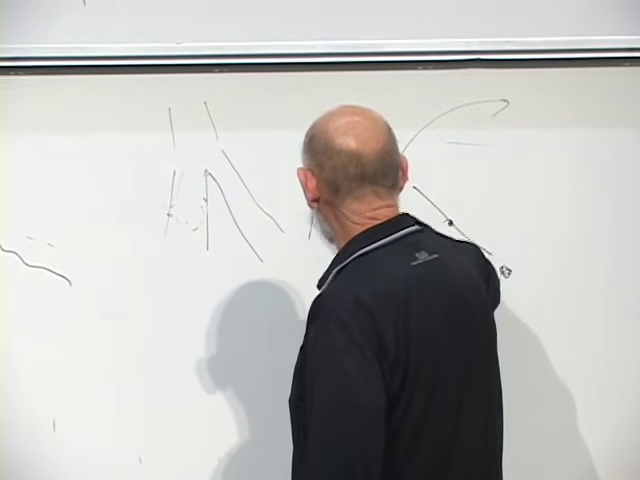
\includegraphics[width=\textwidth]{lecture_03_figure_18.png}
    \par\smallskip\footnotesize (a) 黑板上的结合历史。
  \end{minipage}\hfill
  \begin{minipage}[t]{0.48\textwidth}
    \centering
    \begin{tikzpicture}[>=Latex,scale=0.9]
      \draw[->] (0,-2.1) -- (0,2.2) node[above] {time};
      \draw[blue!70!black,thick] (-2,-1.6) .. controls (-1.3,-0.9)
        and (-0.7,-0.35) .. (0,0);
      \draw[blue!70!black,thick] (2,-1.6) .. controls (1.3,-0.9)
        and (0.7,-0.35) .. (0,0);
      \draw[orange!85!black,thick] (0,0) .. controls (0.25,0.7)
        and (-0.15,1.25) .. (0.15,1.9);
      \fill[red!70!black] (0,0) circle (0.09);
      \node[right] at (0.12,0) {\(g_s\)};
    \end{tikzpicture}
  \end{minipage}
  \caption{端点结合是局部粒子相互作用顶点的弦类似物；时间反演给出分裂。}
  \lectureframe{01:24:05}
  \label{fig:l03-open-vertex}
\end{figure}

耦合是一个振幅。对于一个指定的基本过程，相应的概率从 \(|g_s|^2\) 阶开始，相空间和归一化因子由完整计算提供。因此，把 \(g_s\) 称为 ``概率'' 是非正式的简写；保持振幅与概率的区分可以防止一个虚假的平方。

这种相互作用并不取决于外部弦恰好是在振动、旋转，还是处于某种其他的振子态。那些态会改变具体的矩阵元，但所用的仍是同一条局部连接规则。

\subsection{开弦可以自身闭合}

假设一条开弦的两个端点相遇。连接规则无法知道它们属于同一条弦。它们可以融合，产生一个闭合圈：

\begin{equation}
  \text{open}\longrightarrow\text{closed}.
  \label{eq:l03-self-closing}
\end{equation}

\begin{figure}[H]
  \centering
  \begin{minipage}[t]{0.48\textwidth}
    \centering
    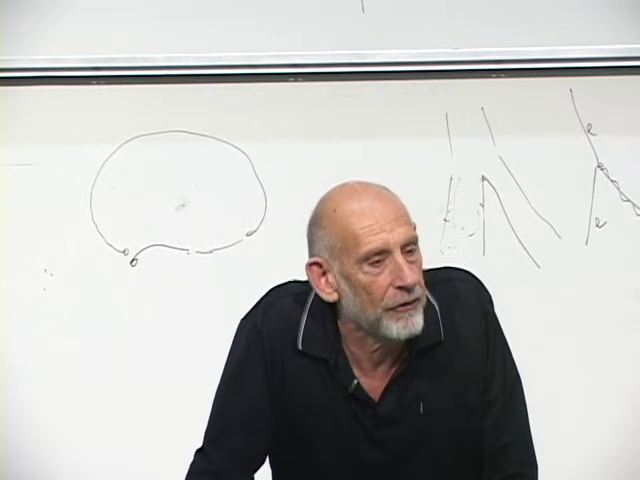
\includegraphics[width=\textwidth]{lecture_03_figure_19.png}
    \par\smallskip\footnotesize (a) 开弦把它的两个端点带到一起。
  \end{minipage}\hfill
  \begin{minipage}[t]{0.48\textwidth}
    \centering
    \begin{tikzpicture}[>=Latex,scale=0.92]
      \draw[blue!70!black,thick]
        (-2,0) .. controls (-1.2,1.5) and (1.2,1.5) .. (2,0);
      \fill[red!70!black] (-2,0) circle (0.08);
      \fill[red!70!black] (2,0) circle (0.08);
      \draw[->,thick] (-0.45,-0.45) -- (0.45,-0.45);
      \draw[orange!85!black,thick] (0,-1.55) ellipse (1.15 and 0.58);
      \node at (0,-2.25) {closed string};
    \end{tikzpicture}
  \end{minipage}
  \caption{相互作用的开弦不可避免地会产生闭弦。}
  \lectureframe{01:27:20}
  \label{fig:l03-open-becomes-closed}
\end{figure}

这不是可有可无的装饰。任何关于相互作用开弦的理论都必须包含闭弦态。逆过程则允许闭弦在存在允许的端点和边界条件时打开成一条开弦。

\begin{classroomqa}
\audiencequestion{当弦融合或分裂时，它们的振子能量会改变吗，理论是否决定了如何改变？\lecturetimestamp{01:28:05}}
\lecturerresponse{会。对于整个过程，能量和动量守恒，而激发可以在出射弦之间重新分配。相互作用顶点和外部波函数决定跃迁振幅。}
\end{classroomqa}

\subsection{闭弦可以在不打开的情况下相互作用}

这一蕴含关系是单向的。相互作用的开弦需要闭弦，但一个理论可以只从闭弦开始。两个闭合圈可以接触、重新连接，并变成一个闭合圈；相反的历史则把一个圈分裂成两个。无需出现任何开端点。

\begin{figure}[H]
  \centering
  \begin{minipage}[t]{0.48\textwidth}
    \centering
    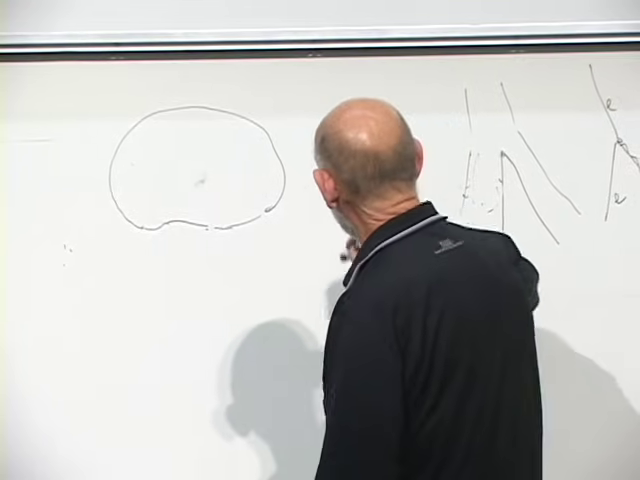
\includegraphics[width=\textwidth]{lecture_03_figure_20.png}
    \par\smallskip\footnotesize (a) 黑板上的闭弦融合。
  \end{minipage}\hfill
  \begin{minipage}[t]{0.48\textwidth}
    \centering
    \begin{tikzpicture}[>=Latex,scale=0.88]
      \draw[blue!70!black,thick] (-1.35,0) circle (0.75);
      \draw[blue!70!black,thick] (1.35,0) circle (0.75);
      \draw[->,thick] (-0.35,-1.15) -- (0.35,-1.15);
      \draw[orange!85!black,thick] (0,-2.3) ellipse (1.35 and 0.68);
      \node at (0,1.2) {closed \(+\) closed};
      \node at (0,-3.25) {closed};
    \end{tikzpicture}
  \end{minipage}
  \caption{闭弦拥有自己的连接与分裂相互作用，无需经过开弦态。}
  \lectureframe{01:29:05}
  \label{fig:l03-closed-fusion}
\end{figure}

\begin{classroomqa}
\audiencequestion{如果一个理论从闭弦开始，它是否也必须包含开弦？\lecturetimestamp{01:28:35}}
\lecturerresponse{不。闭弦可以通过重新连接而相互作用，同时始终保持闭合。开弦需要额外的边界数据，例如允许的端点或膜。}
\end{classroomqa}

\section{为什么引力无法避免}

闭弦振子的计算与开弦的类似，但存在独立的左行和右行激发。它们最低的非平凡匹配能级包含一个无质量的自旋二态。该态具有引力子的螺旋度。因此，每一个自洽的相互作用闭弦理论都包含引力。

\begin{classroomqa}
\audiencequestion{为什么最低的闭弦激发必须是引力子，正如开弦能级必须是类光子的那样？
\lecturetimestamp{01:30:59}}
\lecturerresponse{答案是同一种态计数，现在带有左行和右行振子矢量。它们的张量积包含一个无质量的对称无迹自旋二极化。显式的闭弦谱将在下一步算出；在现阶段，要点是那个态的不可避免性。}
\end{classroomqa}

开弦和闭弦也可以彼此相互作用。一个闭合圈可以遇到一条开弦并被吸收，留下一条更大或激发方式不同的开弦。反过来，一条开弦可以辐射出一个闭合圈。在粒子层面，这就是物质对引力子的发射或吸收。

\begin{figure}[H]
  \centering
  \begin{minipage}[t]{0.48\textwidth}
    \centering
    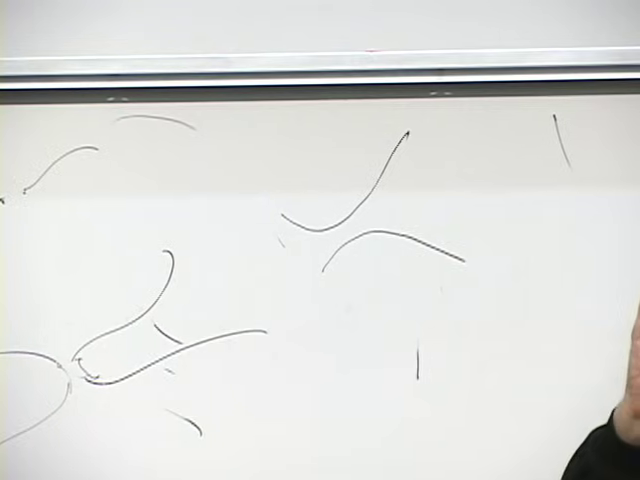
\includegraphics[width=\textwidth]{lecture_03_figure_21.png}
    \par\smallskip\footnotesize (a) 弦段的局部重新连接。
  \end{minipage}\hfill
  \begin{minipage}[t]{0.48\textwidth}
    \centering
    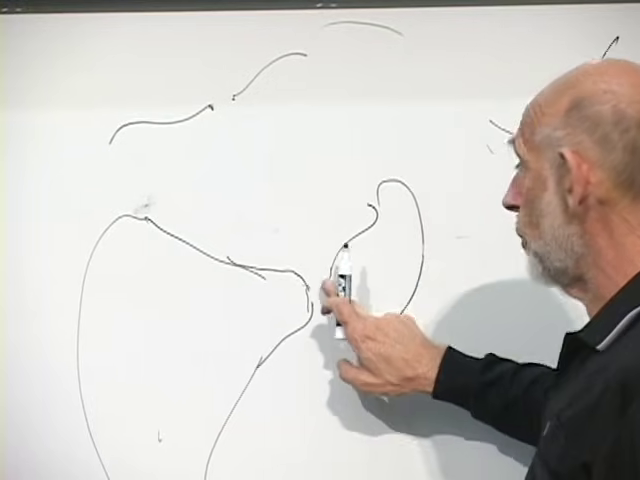
\includegraphics[width=\textwidth]{lecture_03_figure_22.png}
    \par\smallskip\footnotesize (b) 一个闭合圈附着到一条开弦上。
  \end{minipage}
  \caption{混合开--闭相互作用以及引力子交换的普遍可能性背后的黑板图景。
  }
  \lectureframe{01:33:10 and 01:34:35}
\label{fig:l03-mixed-interactions-board}
\end{figure}

\begin{figure}[H]
  \centering
  \begin{tikzpicture}[>=Latex,scale=0.88]
    \draw[blue!70!black,thick]
      (-3,-0.5) .. controls (-1.7,-0.1) and (-0.8,0.2) .. (0,0);
    \draw[blue!70!black,thick]
      (0,0) .. controls (0.9,0.3) and (2.0,0.1) .. (3,0.55);
    \draw[orange!85!black,thick] (-0.8,1.55) ellipse (0.75 and 0.45);
    \draw[->,red!70!black,thick] (-0.45,1.15) -- (-0.05,0.35);
    \node[blue!70!black] at (-2.2,-0.95) {open string};
    \node[orange!85!black] at (-0.8,2.25) {closed string};
    \node at (1.75,-0.5) {excited open string};
  \end{tikzpicture}
  \caption{一幅干净的、不依赖时空的闭弦被开弦吸收的示意图。}
  \label{fig:l03-mixed-interaction-redraw}
\end{figure}

引力子可以耦合到每一种弦态，因为每条弦都携带能量和动量，而且连接规则允许闭弦交换。这就是引力普适性的弦论起源。

\begin{classroomqa}
\audiencequestion{闭弦能否变成开弦，或者能否在不违反端点规则的情况下与开弦结合？\lecturetimestamp{01:31:20}}
\lecturerresponse{在同时包含这两个部分的弦理论中，闭弦可以附着到开弦上并改变其状态。单独一根闭弦能否直接打开，取决于该理论是否提供了允许的端点。局域重联规则保持不变。}
\end{classroomqa}

\begin{classroomqa}
\audiencequestion{闭圈能否永久地相互链接或打结？\lecturetimestamp{01:35:10}}
\lecturerresponse{在弱耦合下弦基本上是透明的：除非很小的重联振幅起作用，它们可以相互穿过。因此链接或结可以在一段时间内持续存在，但当允许的弦相互作用发生时，拓扑可以改变。}
\end{classroomqa}

\begin{classroomqa}
\audiencequestion{相互作用概率是否与弦的状态或速率无关？\lecturetimestamp{01:36:09}}
\lecturerresponse{局域耦合是同一个参数，但总跃迁概率还取决于波函数以及相关部分保持接触的时间长短。快速的相遇通常比缓慢的相遇提供更少的相互作用时间。}
\end{classroomqa}

\section{仍然缺失的标度和耦合}

有两笔账被有意推迟了。第一，\(X\) 是长度，而 \(a_n\) 是无量纲的，因此 \eqref{eq:l03-mode-coordinates} 中的比例关系必须包含一个长度标度。第二，提高振子能级不可能真的把一个无量纲数加到物理质量的平方上。恢复弦长 \(\ell_s\)，或等价地恢复 Regge 斜率 \(\alpha'\sim\ell_s^2\)，就补上了缺失的量纲：

\begin{equation}
  M^2\sim\frac{1}{\alpha'}(N-a).
  \label{eq:l03-dimensional-spectrum}
\end{equation}

精确的约定和归一化将在下一讲中确定。

\begin{classroomqa}
\audiencequestion{是什么确定了弦长的单位和单个产生算符所增加的质量？\lecturetimestamp{01:37:03}}
\lecturerresponse{一个带量纲的常数被省略了。它就是弦标度，通常写作 \(\ell_s\) 或 \(\alpha'\)。振子算符是无量纲的；该标度的幂次把它们的能级数转换为物理长度、张力和质量平方。}
\end{classroomqa}

第二个参数是弦耦合 \(g_s\)。在最简单的讨论中，它是一个控制结合与分裂的普适数。在更丰富的模型中，端点可以携带不同的标记，弦可以在交汇处相遇。Y 形构型是三条通量管相遇的弦类比；在旧强子图像中，它与三夸克重子相关联，而单个开弦段则类似于夸克--反夸克介子。

\begin{classroomqa}
\audiencequestion{不同的弦端点能否具有不同的结合概率？\lecturetimestamp{01:39:31}}
\lecturerresponse{最简单的模型使用一个耦合。更精细的理论把荷或边界标记附着到端点上，然后由选择定则决定哪些结合是允许的。详细构造留待以后，但普适的局域结合思想仍然成立。}
\end{classroomqa}

\begin{classroomqa}
\audiencequestion{弦能否纵向分裂或形成 Y 形交汇？\lecturetimestamp{01:40:01}}
\lecturerresponse{某些弦系统确实允许交汇。它们不是刚才画出的普通双端点分裂过程，而是当理论具有相容的弦荷时才会出现。介子--重子通量管类比是理解这一区别的有用图像。}
\end{classroomqa}

\begin{classroomqa}
\audiencequestion{改变时空维数会改变相互作用耦合吗？\lecturetimestamp{01:42:25}}
\lecturerresponse{维数会改变谱、相空间以及紧致化后得到的有效耦合。基本弦耦合仍然组织微扰展开，但它在低维中的表现取决于额外维的几何和体积。}
\end{classroomqa}

\begin{classroomqa}
\audiencequestion{引力是自由弦一开始运动的原因吗？\lecturetimestamp{01:43:17}}
\lecturerresponse{维持运动不需要力。初始位置和速度指定了一个自由解；惯性使它继续前进。引力或其他力会改变这种运动。追问初始条件的成因是一个独立的问题，不属于局域运动方程的一部分。}
\end{classroomqa}

因此我们得到了三个相互关联的结论。对开弦进行量子化会在其第一激发能级产生一个无质量矢量；其下方的玻色子基态是不稳定的；而相互作用不可避免地引入闭弦，其谱中包含引力。接下来的任务是恢复缺失的标度，并明确地进行闭弦量子化。

\chapter{闭弦、能级匹配与对偶性}

\lectureoverview{闭弦在其两个内禀方向上支持彼此独立的波。对这些波作量子化，乍看之下似乎会使开弦的光子加倍，但弦坐标原点平移下的不变性消去了那些单侧状态。第一个存活下来的能级包含一个无质量的自旋二粒子。随后，改变描述方式这一同样的想法引出了一个更广泛的问题：当耦合常数变化时，说某个对象是基本的究竟意味着什么？}

\section{一个被留作备用的生成元}

在画出闭弦之前，让我们从正则力学中回顾一个事实。设
\begin{equation}
  L=L(q_i,\dot q_i),
\end{equation}
并定义与\(q_i\)共轭的动量为
\begin{equation}
  p_i=\frac{\partial L}{\partial\dot q_i}.
\end{equation}
一个无穷小连续变换可以写成
\begin{equation}
  \delta q_i=\epsilon f_i(q),
  \label{eq:l04-infinitesimal-transformation}
\end{equation}
其中\(\epsilon\)是一个小参数。若该变换是一个对称性，诺特定理便给出一个守恒荷。将坐标位移除以公共参数，即得生成元
\begin{equation}
  Q=\sum_i p_i f_i(q)
   =\frac{1}{\epsilon}\sum_i p_i\,\delta q_i.
  \label{eq:l04-noether-charge}
\end{equation}
在量子力学中，\(Q\)就是生成相应小变换的算符。

\(xy\)平面内的旋转是熟悉的例子。取一种取向选择，
\begin{equation}
  \delta x=\epsilon y,
  \qquad
  \delta y=-\epsilon x,
\end{equation}
而\eqref{eq:l04-noether-charge}就成为角动量，至多相差同一个符号选择。这个具体例子并不重要。重要的是那个模式：动量与无穷小位移缩并便给出生成元。

\begin{figure}[H]
  \centering
  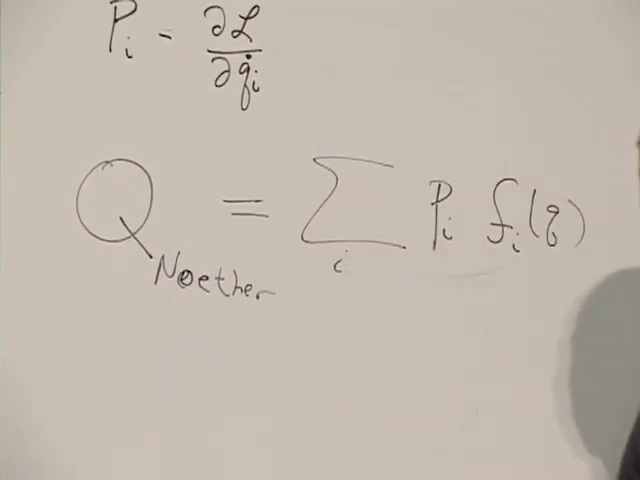
\includegraphics[width=0.76\textwidth]{lecture_04_figure_01.png}
  \caption{为闭弦坐标的后续平移而保留的正则动量与诺特生成元。}
  \lectureframe{00:05:00}
  \label{fig:l04-noether-board}
\end{figure}

我们不久将遇到一个对称性，其坐标不是普通空间中的点，而是弦上各点的标记。式\eqref{eq:l04-noether-charge}正是为此而被置于手边。

\section{环绕一圈的坐标}

闭弦没有端点。选取一个参数
\begin{equation}
  0\leq \sigma<2\pi
\end{equation}
并暂且把某一点标记为\(\sigma=0\)。绕行一半处是\(\sigma=\pi\)；四分之一圈和四分之三圈分别是\(\pi/2\)和\(3\pi/2\)。这个标记确立的是一种坐标约定，尚不是物理特征。

\begin{figure}[H]
  \centering
  \begin{minipage}[t]{0.58\textwidth}
    \centering
    \includegraphics[width=\textwidth]{lecture_04_figure_02.png}
    \par\smallskip\footnotesize (a) 黑板上的带标记的圈。
  \end{minipage}\hfill
  \begin{minipage}[t]{0.37\textwidth}
    \centering
    \begin{adjustbox}{max width=\linewidth}
    \begin{tikzpicture}[scale=0.82]
      \draw[thick]
        (0.1,1.1)
        .. controls (1.0,1.55) and (2.4,1.45) .. (2.9,0.4)
        .. controls (3.25,-0.45) and (2.45,-1.35) .. (1.55,-1.05)
        .. controls (0.65,-1.45) and (-0.35,-1.0) .. (-0.35,-0.05)
        .. controls (-0.35,0.55) and (-0.05,0.9) .. (0.1,1.1);
      \fill (0.1,1.1) circle (1.8pt);
      \node[above] at (0.1,1.12) {\(\sigma=0\)};
      \draw[->,thick] (2.55,0.95) arc[start angle=42,end angle=-25,radius=0.62];
      \node[right] at (3.05,0.55) {increasing \(\sigma\)};
    \end{tikzpicture}
    \end{adjustbox}
    \par\smallskip\footnotesize (b) 内禀取向。
  \end{minipage}
  \caption{标记一个点以定义原点，箭头则固定\(\sigma\)增大的方向。}
  \lectureframe{00:06:48}
  \label{fig:l04-closed-string-origin}
\end{figure}

沿圈的箭头是一种\emph{内禀}取向。切不可把它与\(xy\)平面内的顺时针或逆时针运动相混淆。想象一条带标记的橡皮筋从黑板上被提起、翻面，再放回去。它表观的顺时针方向反转了，而其内禀标记的次序并未反转。\(\sigma\)增大仍然是\(\sigma\)增大。

这一区分支配着右行波与左行波的语言。在本章中，右行扰动指的是朝\(\sigma\)增大的方向传播的扰动，左行扰动指的是朝\(\sigma\)减小的方向传播的扰动。这两个名称都没有告诉我们该扰动在房间里看起来朝哪个方向运动。

取向在最初的强子弦图像中曾起过具体作用。断开一根有取向的流管，会在一端产生一个夸克，在另一端产生一个反夸克；内禀箭头区分了这两端。人们也可以构造无取向的弦理论，但在目前的讨论中，我们保留箭头以及沿它的两个方向。

\section{周期性条件与行波}

设\(X(\sigma,\tau)\)和\(Y(\sigma,\tau)\)为弦的两个横向坐标，\(\tau\)表示时间。若还存在额外的横向坐标，其处理方式完全相同。由于\(\sigma=0\)和\(\sigma=2\pi\)标记的是同一个点，
\begin{equation}
  X(\sigma+2\pi,\tau)=X(\sigma,\tau),
  \qquad
  Y(\sigma+2\pi,\tau)=Y(\sigma,\tau).
  \label{eq:l04-periodicity}
\end{equation}

\begin{figure}[H]
  \centering
  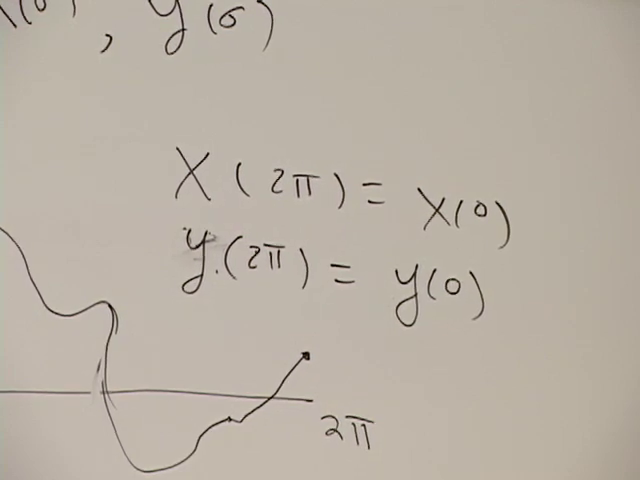
\includegraphics[width=0.76\textwidth]{lecture_04_figure_03.png}
  \caption{两个横向坐标的周期性边界条件。}
  \lectureframe{00:12:40}
  \label{fig:l04-periodicity-board}
\end{figure}

因此，一个局域化的抖动可以无限期地循环传播。当它到达\(2\pi\)时，它就直接在\(0\)处重新出现。这与开弦不同：在开弦上，行波到达端点后会反射；原本左行的变成右行，反之亦然。驻波对开弦来说是自然的，而闭弦则容许两个独立传播的波族。

\subsection{复傅里叶模式}

周期函数的一个便利基是
\begin{equation}
  e^{in\sigma}=\cos(n\sigma)+i\sin(n\sigma),
  \qquad n\in\mathbb Z.
\end{equation}
整数条件由周期性强制给出：
\(e^{in(\sigma+2\pi)}=e^{in\sigma}\)。例如，若把\(n\)替换为半整数，则绕行一周后函数就会改变。

暂时略去时间依赖，黑板上的展开式为
\begin{align}
  X(\sigma)
  &=
  X_0+
  \sum_{n>0}X_n e^{in\sigma}
  +\sum_{n>0}X_{-n}e^{-in\sigma},
  \label{eq:l04-fourier-x}\\
  Y(\sigma)
  &=
  Y_0+
  \sum_{n>0}Y_n e^{in\sigma}
  +\sum_{n>0}Y_{-n}e^{-in\sigma}.
  \label{eq:l04-fourier-y}
\end{align}
对于实的\(X\)和\(Y\)，在经典层面上，负指标系数是正指标系数的复共轭。零模\(X_0\)和\(Y_0\)确定质心位置；它们是位置，而不是内部振动。

\begin{figure}[H]
  \centering
  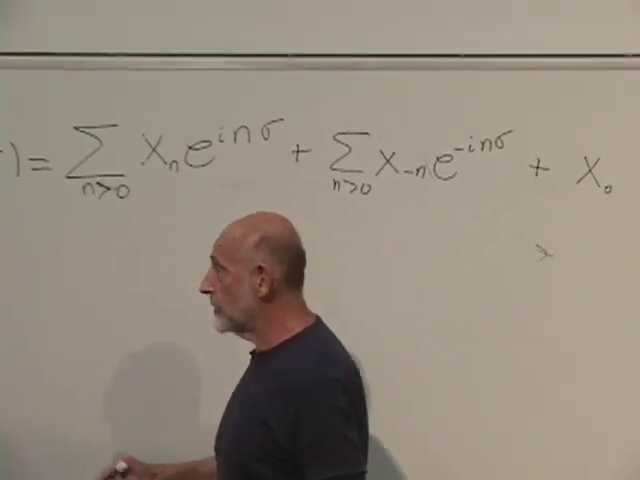
\includegraphics[width=0.82\textwidth]{lecture_04_figure_04.png}
  \caption{周期傅里叶展开的正指标部分与负指标部分，随后是零模。}
  \lectureframe{00:20:00}
  \label{fig:l04-fourier-board}
\end{figure}

\begin{classroomqa}
\audiencequestion{如果这些是行波，那么时间坐标在哪里？\lecturetimestamp{00:19:05}}
\lecturerresponse{它只是在黑板记号中被略去了。行波解携带一个同时涉及\(\sigma\)和\(\tau\)的相位。按照下文所用的约定，一族有
\(e^{-in(\tau-\sigma)}\)，另一族有
\(e^{-in(\tau+\sigma)}\)。}
\end{classroomqa}

因此，决定传播的是完整的相位，而不是单纯空间傅里叶因子中\(n\)的符号本身。我们可以写出
\begin{equation}
  X(\sigma,\tau)=X_R(\tau-\sigma)+X_L(\tau+\sigma),
  \label{eq:l04-chiral-solution}
\end{equation}
对\(Y\)也类似。哪一族被称为\(R\)而不是\(L\)只是一个约定；不变的事实是，沿\(\sigma\)圆有两个相反方向。\editorialnote{某一瞬间的因子\(e^{in\sigma}\)本身并不指定一个行波。只有在给定时间相位之后，传播才被确定。}

\section{两个方向上的能量}

局域动力学与开弦相同。在这里所用的简化归一化下，
\begin{equation}
  L\propto
  \int_0^{2\pi}d\sigma\,
  \left[
    \dot X^2-X'^2+\dot Y^2-Y'^2
  \right],
  \label{eq:l04-string-lagrangian}
\end{equation}
其中点表示\(\partial_\tau\)，撇表示
\(\partial_\sigma\)。能量在动能项与弹性项之间取正号：
\begin{equation}
  E\propto
  \int_0^{2\pi}d\sigma\,
  \left[
    \dot X^2+X'^2+\dot Y^2+Y'^2
  \right].
  \label{eq:l04-string-energy}
\end{equation}
对任一横向坐标，
\begin{equation}
  \dot X^2+X'^2
  =
  \frac12(\dot X+X')^2+
  \frac12(\dot X-X')^2.
  \label{eq:l04-energy-square-completion}
\end{equation}
交叉项相消，恰好留下原来的动能与梯度能量。

\begin{figure}[H]
  \centering
  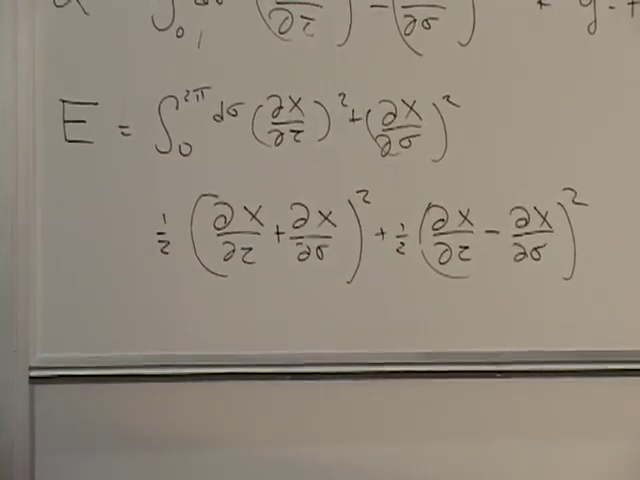
\includegraphics[width=0.82\textwidth]{lecture_04_figure_05.png}
  \caption{总能量被重新组织到两个行波扇区中。}
  \lectureframe{00:25:10}
  \label{fig:l04-energy-board}
\end{figure}

对于\(X_R(\tau-\sigma)\)，有\(\dot X_R=-X_R'\)；对于
\(X_L(\tau+\sigma)\)，有\(\dot X_L=X_L'\)。因此，\eqref{eq:l04-energy-square-completion}中的两个平方项分离出两个手征族。包括每一个横向坐标，定义
\begin{align}
  E_L&\propto
  \frac12\int_0^{2\pi}d\sigma
  \sum_I(\dot X^I+X^{I\prime})^2,\\
  E_R&\propto
  \frac12\int_0^{2\pi}d\sigma
  \sum_I(\dot X^I-X^{I\prime})^2.
  \label{eq:l04-left-right-energies}
\end{align}
于是\(E=E_L+E_R\)。由于在这一阶段方程是线性的，来自两个扇区的波彼此穿过而不发生散射。

\subsection{两倍的振子数}

把傅里叶级数代入
\eqref{eq:l04-string-lagrangian}，会把每个非零模系数变成一个谐振子。其频率正比于\(|n|\)：波长越短，频率越高，因此激发能越大。与开弦不同，每个正频率都以两个独立传播的副本出现。

黑板上把\(X\)极化的产生算符标为
\(a_n^+\)和\(a_{-n}^+\)，把\(Y\)极化的产生算符标为
\(b_n^+\)和\(b_{-n}^+\)。为了更清楚地区分产生与传播，我们将写出
\begin{equation}
  a_n^\dagger,\quad b_n^\dagger,
  \qquad
  \widetilde a_n^\dagger,\quad\widetilde b_n^\dagger,
  \qquad n>0.
  \label{eq:l04-oscillator-notation}
\end{equation}
无波浪号与带波浪号的算符产生相反的世界面方向；
\(a\)和\(b\)表示两个横向极化。

\begin{figure}[H]
  \centering
  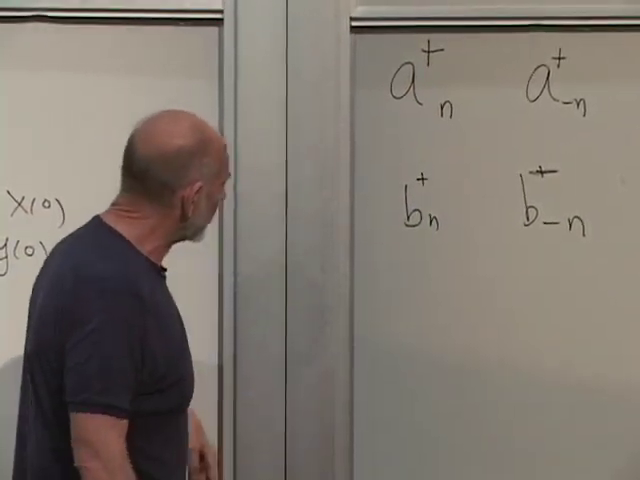
\includegraphics[width=0.65\textwidth]{lecture_04_figure_06.png}
  \caption{黑板记号中加倍后的\(X\)极化和\(Y\)极化产生算符。}
  \lectureframe{00:29:10}
  \label{fig:l04-oscillators-board}
\end{figure}

如果\(N_n^{(a)},N_n^{(b)}\)及其带波浪号的伙伴是占据数，那么两个方向上携带的振子能级示意为
\begin{equation}
  \begin{aligned}
    N&=\sum_{n>0}n\bigl(N_n^{(a)}+N_n^{(b)}+\cdots\bigr),\\
    \widetilde N&=\sum_{n>0}n
      \bigl(\widetilde N_n^{(a)}+\widetilde N_n^{(b)}+\cdots\bigr).
  \end{aligned}
  \label{eq:l04-level-operators}
\end{equation}
省略号表示额外的横向方向。

\section{失败的谱猜测}

回忆开弦的第一能级。用\(a_1^\dagger\)或\(b_1^\dagger\)作用于基态，给出两个线偏振。它们的圆组合，
\begin{equation}
  c_\pm^\dagger
  =
  \frac{1}{\sqrt2}
  \left(a_1^\dagger\pm i b_1^\dagger\right),
  \label{eq:l04-open-circular}
\end{equation}
携带螺旋度\(h=\pm1\)。没有螺旋度为零的伙伴，正是在这个初等四维描述中无质量矢量的标志。

设闭弦基态的质量平方为\(m_0^2\)。第一个朴素的猜测是用
\begin{equation}
  a_1^\dagger,\quad b_1^\dagger,\quad
  \widetilde a_1^\dagger,\quad\widetilde b_1^\dagger.
  \label{eq:l04-naive-one-sided}
\end{equation}
中的任意一个作用一次。这类似于开弦光子的两个副本，每个传播方向一个。然而在下一个能量级，不受限制的列表并不能组装成合理的转动多重态。更精细的记账并不能修复这个问题。认为每个振子单项式都是物理态这一前提是错误的。

\subsection{能级匹配，首先作为一条规则}

物理的闭弦条件是
\begin{equation}
  N=\widetilde N,
  \qquad\text{equivalently}\qquad E_L=E_R.
  \label{eq:l04-level-matching}
\end{equation}
目前先把它当作一个假设；只有在看到它达成了什么之后，才会推导它的起源。

\eqref{eq:l04-naive-one-sided}中的每个态在一个扇区中具有一份能量单位，而在另一个扇区中没有能量单位，因此每一个都被排除。最先存活下来的态从每一族中携带一个振子：
\begin{align}
  a_1^\dagger\widetilde a_1^\dagger\ket{0},
  &\qquad
  b_1^\dagger\widetilde b_1^\dagger\ket{0},
  \label{eq:l04-four-matched-a}\\
  a_1^\dagger\widetilde b_1^\dagger\ket{0},
  &\qquad
  b_1^\dagger\widetilde a_1^\dagger\ket{0}.
  \label{eq:l04-four-matched-b}
\end{align}
它们具有总振子能量二，在两个方向之间均分。单个\(n=2\)产生算符具有相同的总振子能量，但不满足\eqref{eq:l04-level-matching}；它只向一侧贡献两份能量单位。

\begin{figure}[H]
  \centering
  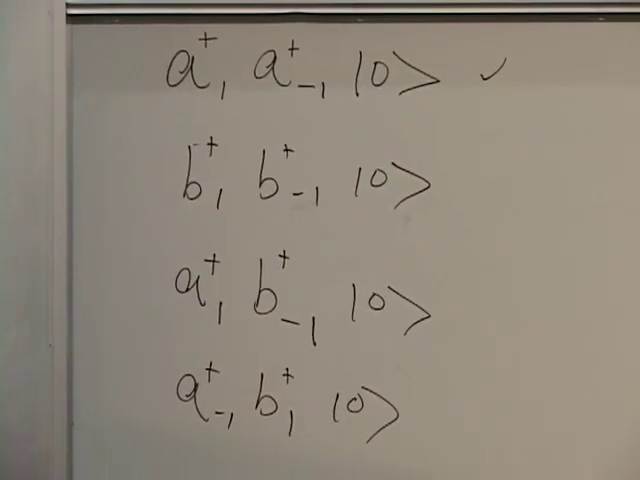
\includegraphics[width=0.70\textwidth]{lecture_04_figure_07.png}
  \caption{存活下来并通过能级匹配的四个第一能级态。图中使用下标\(1\)和\(-1\)，而\eqref{eq:l04-four-matched-a}--\eqref{eq:l04-four-matched-b}使用无波浪号和有波浪号的算符。}
  \lectureframe{00:41:05}
  \label{fig:l04-level-matched-board}
\end{figure}

\section{第一匹配能级中的引力子}

将两个手征族放入圆基：
\begin{equation}
  c_\pm^\dagger
  =\frac{a_1^\dagger\pm i b_1^\dagger}{\sqrt2},
  \qquad
  \widetilde c_\pm^\dagger
  =\frac{\widetilde a_1^\dagger\pm i\widetilde b_1^\dagger}{\sqrt2}.
  \label{eq:l04-closed-circular}
\end{equation}
每个因子在普通横向空间中贡献螺旋度\(+1\)或\(-1\)。因此它们的乘积给出
\begin{center}
\begin{tabular}{c c}
  \toprule
  态&螺旋度\\
  \midrule
  \(c_+^\dagger\widetilde c_+^\dagger\ket0\) & \(+2\) \\
  \(c_-^\dagger\widetilde c_-^\dagger\ket0\) & \(-2\) \\
  \(c_+^\dagger\widetilde c_-^\dagger\ket0\) & \(0\) \\
  \(c_-^\dagger\widetilde c_+^\dagger\ket0\) & \(0\) \\
  \bottomrule
\end{tabular}
\end{center}

\begin{classroomqa}
\audiencequestion{第二个圆偏振因子是否应来自相反的传播扇区？\lecturetimestamp{00:43:20}}
\lecturerresponse{是的。黑板上写下的第一个表达式正是因为这个原因而被更正。这里的物理态必须将一个右行振子与一个左行振子配对；否则它就不是能级匹配的。螺旋度指的是横向空间偏振，而这两个因子指的是相反的世界面方向。}
\end{classroomqa}

\begin{figure}[H]
  \centering
  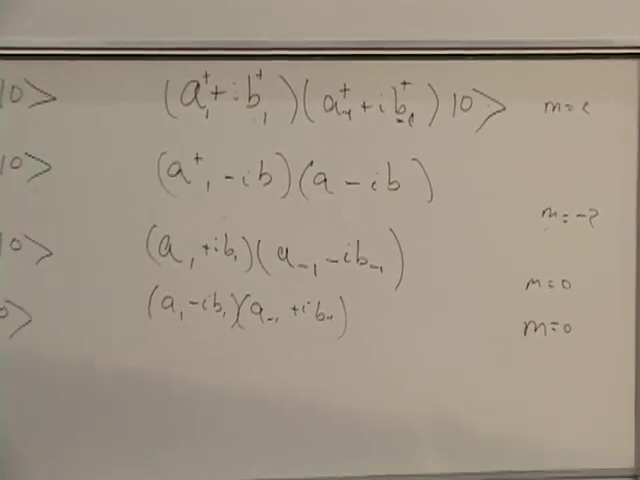
\includegraphics[width=0.82\textwidth]{lecture_04_figure_08.png}
  \caption{黑板更正后的四个圆基乘积，其螺旋度为\(+2,-2,0,0\)。}
  \lectureframe{00:46:10}
  \label{fig:l04-helicity-board}
\end{figure}

有质量的自旋二粒子有五个自旋投影，
\begin{equation}
  m=2,1,0,-1,-2.
\end{equation}
匹配能级不包含\(m=\pm1\)伙伴。因此它不可能是有质量的自旋二多重态。相比之下，无质量的自旋二粒子只有螺旋度\(+2\)和\(-2\)。同螺旋度乘积恰好就是这两个态：它们就是引力子偏振。

还剩下两个螺旋度为零的组合。用课上使用的语言来说，一个是膨胀子，另一个是轴子。对一般闭玻色弦的协变描述细化了这一陈述：
\begin{equation}
  \begin{aligned}
    \alpha_{-1}^{I}\widetilde\alpha_{-1}^{J}\ket{0;k}
    &\longrightarrow
    \underbrace{h_{IJ}}_{\text{symmetric traceless}}
    \oplus
    \underbrace{B_{IJ}}_{\text{antisymmetric}}\\
    &\hspace{2.5em}\oplus
    \underbrace{\Phi}_{\text{trace}}.
  \end{aligned}
  \label{eq:l04-massless-tensor-decomposition}
\end{equation}
这些是引力子、反对称二形式和膨胀子。在四维中，二形式可以对偶化为类轴子赝标量，这就是讲座中采用的语言。\editorialnote{第二个螺旋度为零的态在一般闭弦谱中从根本上就是反对称张量场\(B_{\mu\nu}\)。称其为轴子是四维对偶描述。}

在这个形式层面上，这三个场是无质量的。紧致化、投影和背景动力学可以改变哪些标量或二形式自由度保持轻。引力子则不同：一旦存在一个自洽的相互作用闭弦扇区，其无质量自旋二态就是不可避免的。这就是为什么引力从闭弦中涌现，而不是作为单独的成分被附加进去。

\section{为什么能级必须匹配}

我们现在回到\(\sigma=0\)处的标记。它是附着在圈上的物理珠子，还是仅仅是我们参数的起点？对于一条普通的无标记闭弦，不应有任何点享有特权。当所有标签一起平移时，量子态必须保持不变。

\subsection{离散版本}

将圈正则化为\(M\)个有序点，其横向坐标为\((X_i,Y_i)\)。暂时抑制\(Y_i\)。一个位形空间波函数是
\begin{equation}
  \Psi(X_1,X_2,\ldots,X_M).
\end{equation}
改变哪个点被称为第一个给出一个循环置换：
\begin{align}
  \Psi(X_1,X_2,\ldots,X_M)
  &=
  \Psi(X_2,\ldots,X_M,X_1)\nonumber\\
  &=
  \Psi(X_3,\ldots,X_M,X_1,X_2).
  \label{eq:l04-cyclic-wavefunction}
\end{align}
这不是在任意置换下的不变性。例如，在\(X_1\)和\(X_2\)之间插入\(X_3\)会改变邻接结构，并有效地撕裂和重新连接离散化的弦。只有共同的循环重标记
\begin{equation}
  X_i\longrightarrow X_{i+1}\qquad(\text{mod }M)
  \label{eq:l04-discrete-shift}
\end{equation}
表达了不存在优先起点。

\begin{figure}[H]
  \centering
  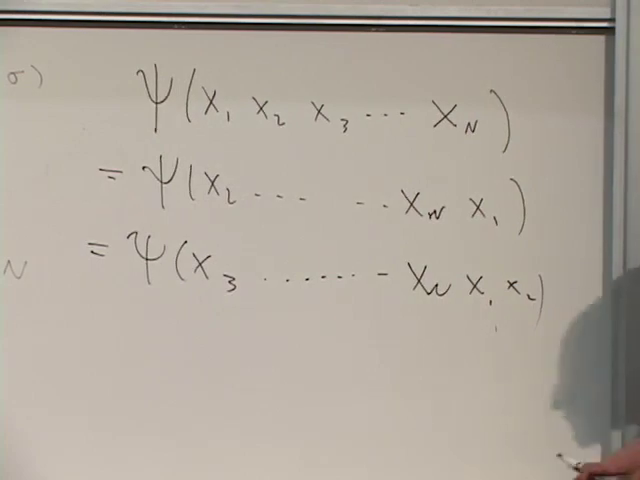
\includegraphics[width=0.82\textwidth]{lecture_04_figure_09.png}
  \caption{离散化闭弦的循环波函数恒等式。}
  \lectureframe{00:56:20}
  \label{fig:l04-cyclic-board}
\end{figure}

\subsection{连续版本}

在连续极限\(M\to\infty\)下，态是波泛函
\begin{equation*}
  \Psi[X(\sigma),Y(\sigma)].
\end{equation*}
循环重标记变为
\begin{equation}
  \sigma\longrightarrow\sigma+\epsilon.
\end{equation}
不变性表明
\begin{equation}
  \Psi[X(\sigma+\epsilon),Y(\sigma+\epsilon)]
  =
  \Psi[X(\sigma),Y(\sigma)].
  \label{eq:l04-wavefunctional-invariance}
\end{equation}

\begin{figure}[H]
  \centering
  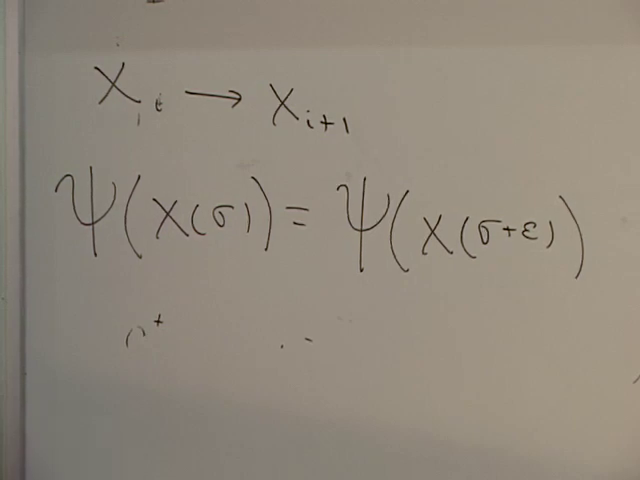
\includegraphics[width=0.72\textwidth]{lecture_04_figure_10.png}
  \caption{离散平移及其波泛函连续形式。}
  \lectureframe{00:58:40}
  \label{fig:l04-wavefunctional-board}
\end{figure}

在一阶近似下，
\begin{equation}
  \delta X(\sigma)=\epsilon X'(\sigma),
  \qquad
  \delta Y(\sigma)=\epsilon Y'(\sigma),
  \label{eq:l04-profile-shift}
\end{equation}
直到区分剖面的主动平移与坐标的被动平移的那个整体符号。相应的波泛函变分为
\begin{equation}
  \delta\Psi
  =
  \epsilon\int_0^{2\pi}d\sigma
  \left[
    \frac{\delta\Psi}{\delta X(\sigma)}X'(\sigma)
    +
    \frac{\delta\Psi}{\delta Y(\sigma)}Y'(\sigma)
  \right].
  \label{eq:l04-functional-variation}
\end{equation}

\begin{figure}[H]
  \centering
  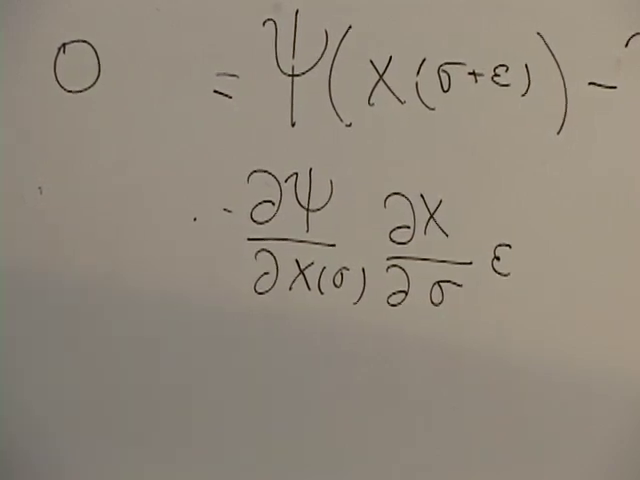
\includegraphics[width=0.72\textwidth]{lecture_04_figure_11.png}
  \caption{平移后波泛函自变量的一阶展开。}
  \lectureframe{01:01:31}
  \label{fig:l04-functional-expansion-board}
\end{figure}

\begin{classroomqa}
\audiencequestion{一阶条件是对\(\sigma\)的每一个值分别成立的独立方程吗？\lecturetimestamp{01:01:30}}
\lecturerresponse{不是。该变换将弦的每一点一起平移。某一点的变分必须与所有其他点的变分相加，这就是连续表达式包含对\(\sigma\)的积分的原因。}
\end{classroomqa}

在坐标表象中，
\begin{equation}
  P_X(\sigma)=-i\frac{\delta}{\delta X(\sigma)},
  \qquad
  P_Y(\sigma)=-i\frac{\delta}{\delta Y(\sigma)}
  \label{eq:l04-functional-momenta}
\end{equation}
其中\(\hbar=1\)。因此方程\eqref{eq:l04-functional-variation}由下式生成：
\begin{equation}
  G_\sigma=
  \int_0^{2\pi}d\sigma\,
  \left[
    P_X(\sigma)X'(\sigma)+P_Y(\sigma)Y'(\sigma)
  \right].
  \label{eq:l04-sigma-generator}
\end{equation}
这正是Noether模式\eqref{eq:l04-noether-charge}：正则动量乘以坐标位移，并对所有自由度求和。一个无标记的闭弦态满足
\begin{equation}
  G_\sigma\ket{\mathrm{phys}}=0.
  \label{eq:l04-physical-generator-condition}
\end{equation}

对于\eqref{eq:l04-string-lagrangian}的归一化，
\(P_I\propto\dot X^I\)，因此同一条件可写为
\begin{equation}
  \int_0^{2\pi}d\sigma
  \sum_I\dot X^I X^{I\prime}=0.
  \label{eq:l04-momentum-constraint}
\end{equation}

\begin{figure}[H]
  \centering
  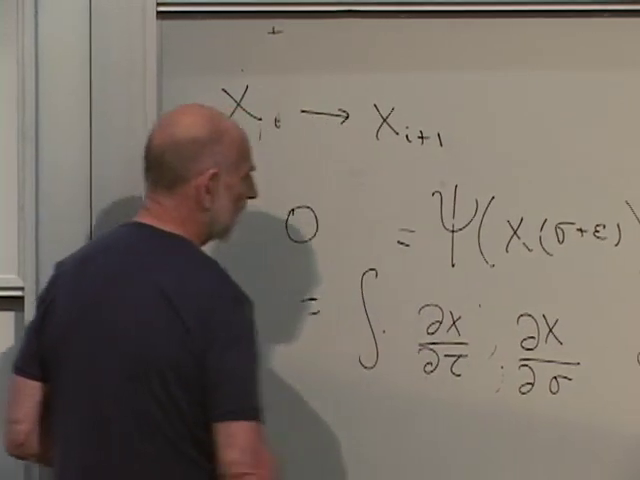
\includegraphics[width=0.75\textwidth]{lecture_04_figure_12.png}
  \caption{在波泛函的导数被等同于动量之后，积分后的生成元。}
  \lectureframe{01:05:10}
  \label{fig:l04-generator-board}
\end{figure}

\subsection{生成元是能量差}

\eqref{eq:l04-left-right-energies}中两个表达式之和是总能量。它们的差为
\begin{align}
  E_L-E_R
  &\propto
  \frac12\int_0^{2\pi}d\sigma\sum_I
  \left[
    (\dot X^I+X^{I\prime})^2\right.\nonumber\\[-0.25em]
  &\hspace{7em}\left.
    -(\dot X^I-X^{I\prime})^2
  \right]\\
  &=
  2\int_0^{2\pi}d\sigma\sum_I
  \dot X^I X^{I\prime}.
  \label{eq:l04-energy-difference}
\end{align}
该积分就是必须湮灭物理态的生成元。因此
\begin{equation}
  E_L-E_R=0,
  \qquad\text{or}\qquad
  N-\widetilde N=0.
\end{equation}
能级匹配所陈述的是：\(\sigma\)坐标的原点是不可观测的。

\begin{figure}[H]
  \centering
  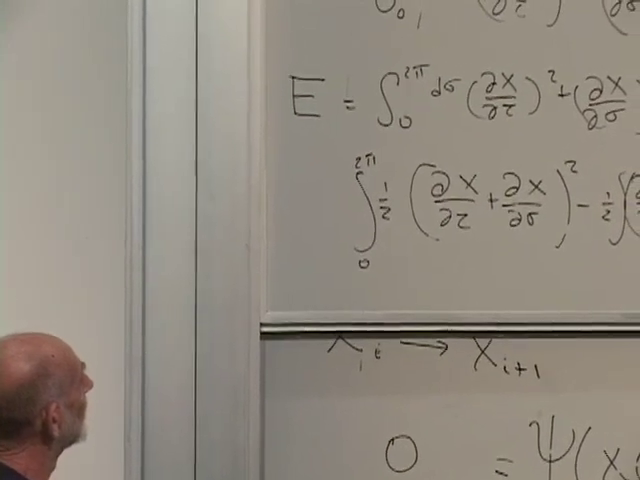
\includegraphics[width=0.78\textwidth]{lecture_04_figure_13.png}
  \caption{在能级匹配推导末尾一起展示的能量之和与能量之差。}
  \lectureframe{01:06:40}
  \label{fig:l04-energy-difference-board}
\end{figure}

\begin{classroomqa}
\audiencequestion{为什么这些展示的公式似乎把二分之一因子的位置放得不同？\lecturetimestamp{01:06:28}}
\lecturerresponse{这里只用到相对结构。恢复一个一致的整体归一化，就得到配平方恒等式\eqref{eq:l04-energy-square-completion}中的二分之一。求和给出总能量，而差值仍正比于
\(\int d\sigma\,\dot X X'\)。它的消失，从而能级匹配，与那个共同的约定无关。}
\end{classroomqa}

该约束去掉了朴素振子谱的很大一部分，而且恰好去掉了那些未能形成合理粒子多重态的态。它并不去掉开弦光子，因为开弦不具有两个受此闭弦回路条件约束的独立循环扇区。对于闭弦，它保留了引力子、膨胀子、反对称张量态或类轴子态，以及更高的匹配能级。
\editorialnote{在协变弦量子化中，能级匹配是零模条件\(L_0-\widetilde L_0=0\)，即世界面约束系统中的一个成员。这里的推导揭示了它的直观起源：闭弦绕圈平移下的不变性。}

\section{左与右的两种含义}

现在“手性”语言有两种互不相关的用法：
\begin{enumerate}
  \item \(X_R(\tau-\sigma)\)与\(X_L(\tau+\sigma)\)描述沿内禀\(\sigma\)圆朝相反方向的传播。
  \item \(c_+^\dagger\)与\(c_-^\dagger\)描述物理横向\(xy\)平面中的圆偏振。
\end{enumerate}
能级匹配的引力子态包含来自每个世界面方向的一个振子。然而这两个振子可以具有相同的时空螺旋度，从而产生\(h=+2\)或\(h=-2\)。混淆这两种左与右，会使谱看起来自相矛盾，而实际上并非如此。

\section{基本是什么意思？}

一旦开弦和闭弦在这个初等层面上被量子化，一个自然的问题仍然存在：弦是最终组分吗，还是它们本身也可能由别的东西构成？

\begin{classroomqa}
\audiencequestion{是否有证据或理由把弦视为最基本客体，其下没有更小的东西？\lecturetimestamp{01:10:44}}
\lecturerresponse{不存在有用的、与参数无关的答案。在某一区域看起来基本的自由度，在另一区域可能变得重、延展，并且显得像是复合的。最好把“基本”理解为关于在所考虑的耦合下哪些变量提供了有用描述的陈述。}
\end{classroomqa}

电荷与磁荷为这一答案提供了最干净的模型。假设一个理论包含电荷 \(e\) 和磁荷 \(g\)。附着在单极子上的不可观测的狄拉克弦要求
\begin{equation}
  eg=2\pi n,
  \qquad n\in\mathbb Z.
  \label{eq:l04-dirac-quantization}
\end{equation}
对于最小电荷，\(n=1\)。一个绕狄拉克弦运动的带电粒子随后获得相位 \(e^{ieg}=1\)，因此这条辅助弦无法被探测到。

\begin{figure}[H]
  \centering
  \begin{minipage}[t]{0.58\textwidth}
    \centering
    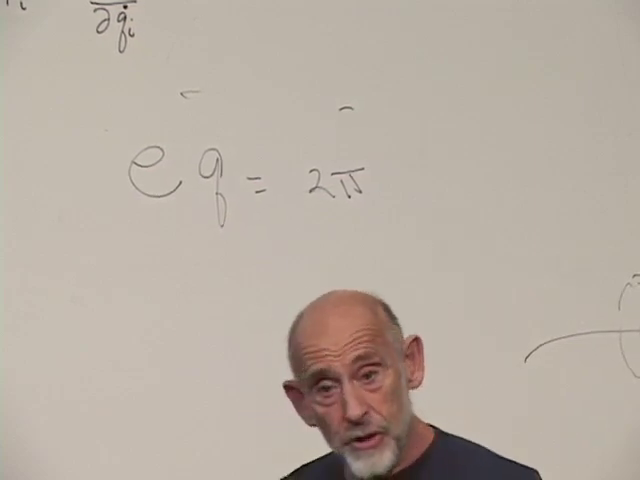
\includegraphics[width=\textwidth]{lecture_04_figure_14.png}
    \par\smallskip\footnotesize (a) 黑板上的狄拉克量子化。
  \end{minipage}\hfill
  \begin{minipage}[t]{0.36\textwidth}
    \centering
    \begin{adjustbox}{max width=\linewidth}
    \begin{tikzpicture}[scale=0.85]
      \fill (0,0) circle (2.5pt);
      \node[above left] at (0,0) {monopole \(g\)};
      \draw[thick] (0,0) -- (3.0,0);
      \node[below] at (1.5,0) {Dirac string};
      \draw[->,thick] (1.5,0.15) arc[start angle=205,end angle=-145,
        x radius=0.8,y radius=0.55];
      \node[right] at (2.15,0.8) {charge \(e\)};
    \end{tikzpicture}
    \end{adjustbox}
    \par\smallskip\footnotesize (b) 围绕弦的相位实验。
  \end{minipage}
  \caption{电荷与磁荷通过狄拉克条件成反比关系。}
  \lectureframe{01:13:20}
  \label{fig:l04-dirac-board}
\end{figure}

如果 \(e\) 很小，则以电变量进行的普通微扰论是有用的。带有额外电顶点的费曼图受到越来越强的压低。但 \eqref{eq:l04-dirac-quantization} 随后使 \(g\) 变大，因此以磁顶点进行的图解展开并不有用。用通常的无量纲耦合常数表示，
\begin{equation}
  \alpha_e=\frac{e^2}{4\pi},
  \qquad
  \alpha_m=\frac{g^2}{4\pi},
  \qquad
  \alpha_e\alpha_m=\frac{n^2}{4}.
  \label{eq:l04-dual-couplings}
\end{equation}
弱电耦合就是强磁耦合，反之亦然。

强耦合的单极子从电的描述来看也显得复杂。它的场能很大；它被强烈的规范场涨落云和虚的带磁荷对所包裹。它表现为一个沉重的、延展的客体，是电微扰级数的一个糟糕出发点。这并不证明它不那么基本。它只是说，对于那个区域而言，它是错误的初等变量。

现在想象连续增大 \(e\)。量子化条件迫使 \(g\) 减小。在自对偶区域附近，两种描述都不特别弱，而越过该区域后，磁变量可以成为更简单、更轻的变量，而电客体则变得被强烈包裹。哪个电荷应被称为基本电荷已经改变，而理论的物理内容并未改变。

\subsection{维格纳之问}

这一模糊性曾在关于希格斯玻色子是基本的还是复合的讨论中浮现出来。尤金·维格纳反复追问复合意味着什么。一个被提出的区分是衰变：也许基本客体不能衰变，而复合客体可以。但基态氢原子不能衰变，却显然是复合的；质子可能稳定而中子衰变，然而这并不使其中一个成为基本的、另一个成为所意指意义上的复合的。每一个简单的定义都产生了另一个反例。

赫拉尔杜斯·特霍夫特以操作性的判据结束了讨论：当一个客体把它想成基本的很有用时，它就是基本的。这不是回避。它承认，基本一词标识的是动力学在其中简单的那些变量，而简单性可以依赖于耦合和环境。

\section{走向M理论}

弦理论以特别鲜明的方式实现了这种角色的交换。在一个参数区域中，弦是轻的且是微扰的，而D膜看起来像是由弦自由度构成的沉重孤子式复合体。随着参数变化，D膜可以成为更轻的基本客体，而在第一个区域中被描述为弦的位形可以用它们来重新解释。看起来基本的可以变成复合的；看起来复合的可以变成基本的。

旧的还原论图景暗示着从大的事物到更小的组分、最终到唯一底层的一种单向下降。对偶性暗示着某种不那么线性的东西：描述可以随着耦合变化而相互转化，没有任何单一组变量在所有地方都享有特权。这正是接近下一个主题——M理论——的视角。

为什么玻色弦的临界维数是二十六、超弦的临界维数是十，这些问题在此仍然悬而未决。与其在继续前进之前解决每一个技术问题，我们现在改变视角，追问M理论如何能在适当的极限下产生弦理论。

\chapter{尺度、弦与二十六维}

\lectureoverview{是什么决定了弦谱的间距？答案是张力，一个具有质量平方量纲的量。对于基本弦而言，这一观察将我们引向普朗克单位、直接激发的实际不可能性，以及强引力的出现。经过一段有意的中断之后，我们回到玻色开弦基态。对其零点能进行正规化，便给出了历史上那条\emph{容易}的途径，通向二十四个横向方向，从而通向二十六维时空。}

\section{我们此前略去的尺度}

到目前为止，我们谈论了振动和旋转的弦，却没有说明一个单位的激发意味着什么。一个强子可以被描绘成一根弦，它的振子可以被激发，但从一个态到下一个态的跃迁有多大？是什么决定了它？

在基本弦模型中只有一个有量纲的参数。要找到它，先从一根普通的拉伸弹簧开始。如果其两端相距\(\ell\)，胡克定律给出
\begin{equation}
  E_{\mathrm{spring}}=\frac{k\ell^2}{2}.
  \label{eq:l05-hooke}
\end{equation}
这个二分之一因子是在第一版写出之后由全班补上的。在这个开篇估计中，没有什么本质性的东西会依赖于这类数值因子。

\begin{figure}[H]
  \centering
  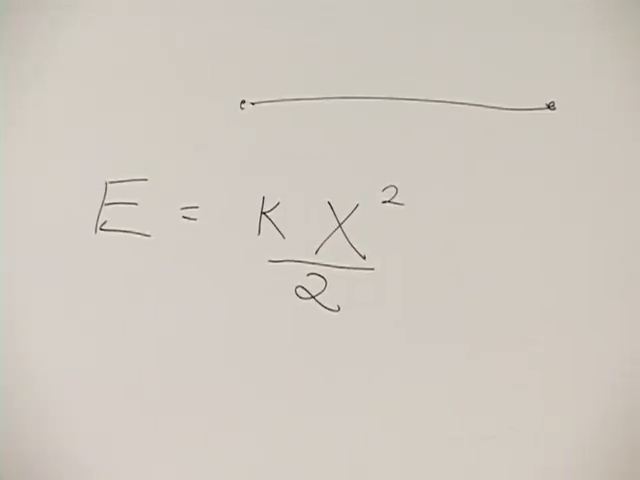
\includegraphics[width=0.72\textwidth]{lecture_05_figure_01.png}
  \caption{拉伸的线段及其胡克定律势能。}
  \lectureframe{00:02:28}
  \label{fig:l05-hooke-board}
\end{figure}

\eqref{eq:l05-hooke}中的能量是非相对论性的。在前几讲所用的无限动量描述中，内部非相对论能量并不正比于\(m\)，而是正比于\(m^2\)。因此我们示意性地写出
\begin{equation}
  m^2\sim k\ell^2,
  \qquad
  m\sim \sqrt{k}\,\ell.
  \label{eq:l05-mass-length}
\end{equation}
在弦的静止系中，其质量就是其能量，所以第二个关系式具有如下形式
\begin{equation}
  E_{\mathrm{rest}}\sim T_s\ell,
  \qquad
  T_s\equiv\sqrt{k}.
  \label{eq:l05-tension}
\end{equation}
系数\(T_s\)就是弦张力：单位长度所储存的能量。

\begin{figure}[H]
  \centering
  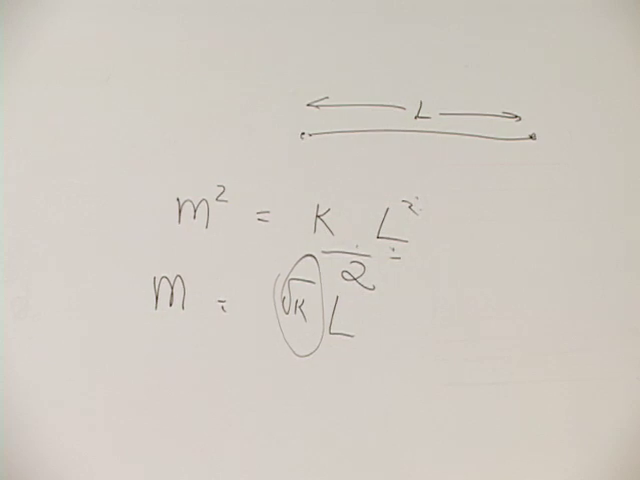
\includegraphics[width=0.78\textwidth]{lecture_05_figure_02.png}
  \caption{黑板从\(m^2\sim k\ell^2\)过渡到正比于长度的质量。}
  \lectureframe{00:05:42}
  \label{fig:l05-mass-length-board}
\end{figure}

这套记号是为本讲的弹簧类比而改写的。在标准的相对论性弦记号中，人们通常写出
\begin{equation}
  T_s=\frac{1}{2\pi\alpha'},
  \label{eq:l05-alpha-prime}
\end{equation}
于是弦能级的增量产生量级为\(1/\alpha'\)的\(m^2\)增量，等价地说，量级为张力。
\editorialnote{本讲中有效的\(k\)被选得使\(\sqrt{k}\)扮演张力的角色。与约定无关的陈述是：\(T_s\)具有质量平方的量纲，并且雷吉斜率满足\(\alpha'\propto T_s^{-1}\)。}

\subsection{量纲与振子能隙}

令\(c=\hbar=1\)。能量于是具有长度倒数的量纲：
\begin{equation}
  [E]=L^{-1}.
\end{equation}
由于张力是单位长度的能量，
\begin{equation}
  [T_s]=L^{-2}=E^2.
  \label{eq:l05-tension-dimension}
\end{equation}
这就是为什么弦谱自然地以质量平方为间距。

\begin{figure}[H]
  \centering
  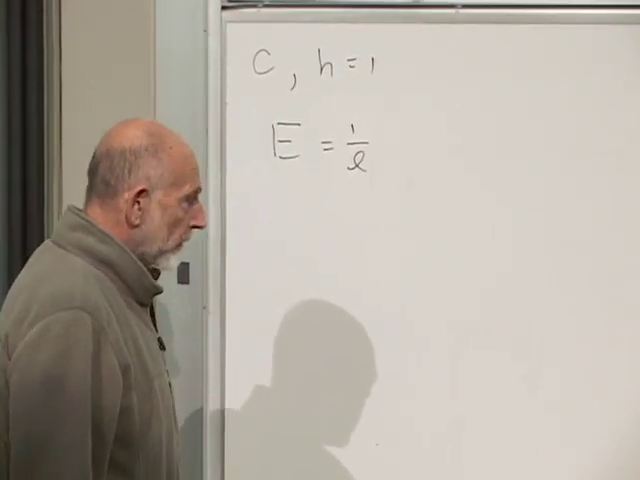
\includegraphics[width=0.68\textwidth]{lecture_05_figure_03.png}
  \caption{黑板上的自然单位：\(c=\hbar=1\)，能量是长度倒数，而振子频率由弹簧尺度控制。}
  \lectureframe{00:06:05}
  \label{fig:l05-natural-units-board}
\end{figure}

普通的振子从另一个方向说明了同一点。对于质量为\(\mu\)的弹簧，
\begin{equation}
  \omega=\sqrt{\frac{k}{\mu}},
  \qquad
  \Delta E=\hbar\omega.
\end{equation}
更硬的弹簧有更高的频率和更大的量子能隙。一根弦包含无穷多个这样的简正模，但它们的共同尺度由\(T_s\)固定。一旦张力已知，弦谱的间距也就已知了。

张力也具有力的量纲，因为力乘以距离就是能量。想象把一端固定，从另一端悬挂一个重物。一根满足\(E=T_s\ell\)的理想相对论性弦能够支撑一个由\(T_s\)设定的力，与它的长度无关。在这个刻意虚构的比较中，由观测到的激发能推断出的强子张力，相当于一辆卡车的重量。从来没有卡车被悬挂在介子上；测得的谱给出张力，而张力给出这一力学比较。

基本弦会硬得多。如果它们构成了电子、光子和引力子的基础，那么它们的第一次振子激发必定远高于观测到的粒子能量。在同一个虚构的引力实验中，它们的张力可以支撑星系量级的东西。这一比较的要点不在于工程。而在于：巨大的张力既意味着很大的激发能，也意味着极小的基态涨落。

\section{由普适常数构成的单位}

多大的尺度才算足够巨大？自然的基准是普朗克尺度。与其引用它，不如让我们把它构造出来。

米、千克和秒是极好的实验室单位，但它们的起源却是人体尺度。米适合量布或绳子；英尺得名于身体的一部分；秒则是一天的可操作分数。人们可以把质子半径设为1，从而简化某些核公式，但质子只是一种特定的复合粒子。这样的选择不会简化整个物理学。

三个量纲常数具有更普遍的作用范围：
\begin{itemize}
  \item \(c\) 为每个物质系统设定了极限速度；
  \item \(\hbar\) 出现在每个量子系统的不确定关系之中；
  \item \(G\) 将引力与每一种形式的质能耦合起来。
\end{itemize}
选择使 \(c=\hbar=G=1\) 的单位，等价于由这些常数构造出长度、时间和质量的单位。

它们的通常量纲为
\begin{equation}
  \begin{aligned}
    [c]&=LT^{-1},
    & [\hbar]&=ML^2T^{-1},\\
    [G]&=L^3M^{-1}T^{-2}.
  \end{aligned}
  \label{eq:l05-dimensions-constants}
\end{equation}
中间的关系直接来自
\(\Delta x\,\Delta p\gtrsim\hbar\)。最后一条则例如来自
\begin{equation}
  a=\frac{GM}{r^2}.
\end{equation}

\begin{figure}[H]
  \centering
  \begin{minipage}[t]{0.48\textwidth}
    \centering
    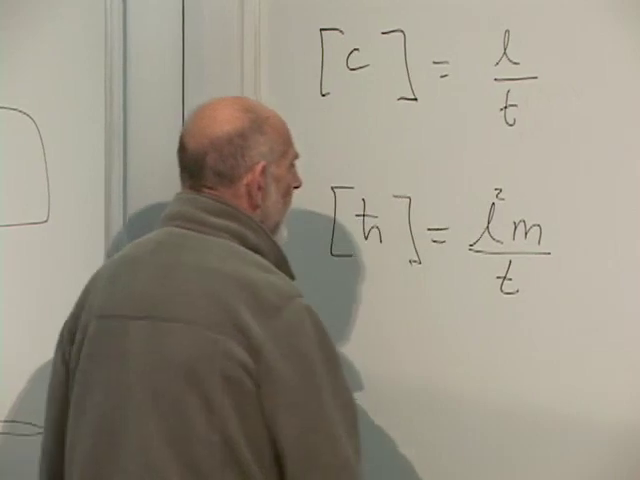
\includegraphics[width=\textwidth]{lecture_05_figure_04.png}
    \par\smallskip\footnotesize (a) \(c\) 和 \(\hbar\) 的单位。
  \end{minipage}\hfill
  \begin{minipage}[t]{0.48\textwidth}
    \centering
    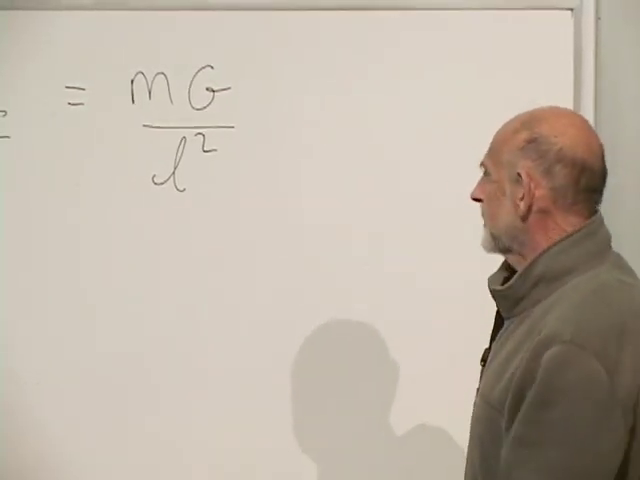
\includegraphics[width=\textwidth]{lecture_05_figure_05.png}
    \par\smallskip\footnotesize (b) 由牛顿加速度得到的 \(G\) 的单位。
  \end{minipage}
  \caption{课堂上汇集起来的量纲分析要素。}
  \lectureframe{00:25:43--00:26:40}
  \label{fig:l05-dimensional-analysis-board}
\end{figure}

\subsection{普朗克面积优先}

寻找幂次 \(p,q,r\)，使得
\begin{equation}
  G^p\hbar^q c^r
\end{equation}
具有量纲 \(L^2\)。优先选择面积可以避免过早出现平方根，也预示了面积日后在引力中将扮演的特殊角色。由
\eqref{eq:l05-dimensions-constants}，质量和时间的抵消给出
\begin{equation}
  -p+q=0,
  \qquad
  -2p-q-r=0.
\end{equation}
剩余的长度幂次必须满足
\begin{equation}
  3p+2q+r=2.
\end{equation}
因此 \(q=p\)、\(r=-3p\) 和 \(p=1\)。普朗克面积为
\begin{equation}
  \ell_P^2=\frac{G\hbar}{c^3},
  \label{eq:l05-planck-area}
\end{equation}
从而
\begin{equation}
  \ell_P=\sqrt{\frac{G\hbar}{c^3}},
  \qquad
  t_P=\frac{\ell_P}{c},
  \qquad
  m_P=\sqrt{\frac{\hbar c}{G}}.
  \label{eq:l05-planck-units}
\end{equation}

\begin{figure}[H]
  \centering
  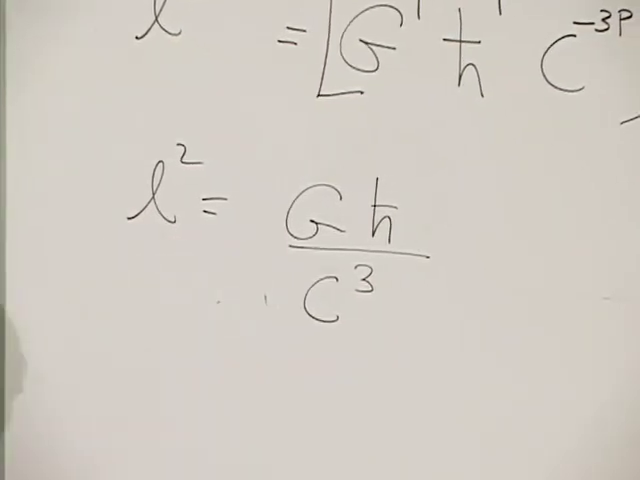
\includegraphics[width=0.78\textwidth]{lecture_05_figure_06.png}
  \caption{关于普朗克面积和长度的完整量纲论证。}
  \lectureframe{00:31:34}
  \label{fig:l05-planck-area-board}
\end{figure}

在数量级精度下，
\begin{equation}
  \begin{aligned}
    \ell_P&\sim10^{-35}\,\mathrm{m},
    &t_P&\sim10^{-43}\,\mathrm{s},\\
    m_P&\sim10^{-8}\,\mathrm{kg},
    &m_Pc^2&\sim10^{19}\,\mathrm{GeV}.
  \end{aligned}
  \label{eq:l05-planck-numbers}
\end{equation}

\begin{figure}[H]
  \centering
  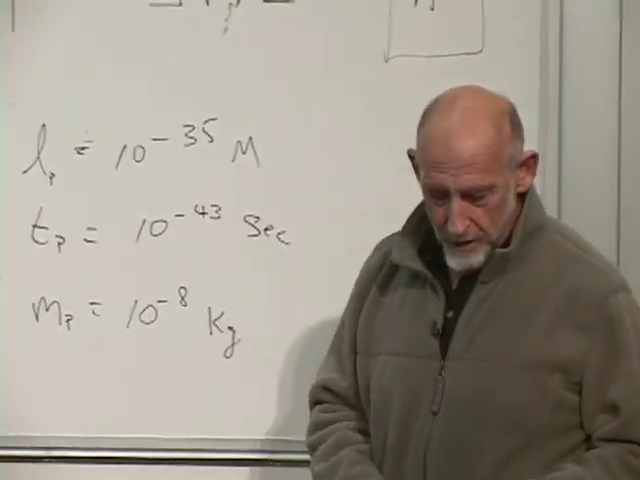
\includegraphics[width=0.72\textwidth]{lecture_05_figure_07.png}
  \caption{按数量级记录下来的三个普朗克尺度。}
  \lectureframe{00:35:12}
  \label{fig:l05-planck-values-board}
\end{figure}

长度和时间小得无法想象，而质量按粒子标准来看却大得惊人，大致相当于一粒细尘埃的质量。它的静能约为几吉焦，与一箱汽油中的化学能相当。相比之下，可观测宇宙大约跨越 \(10^{60}\) 个普朗克长度，并且已经存在了大约 \(10^{60}\) 个普朗克时间。这些比较意在赋予这些单位以物理分量，而不是提高它们的数值精度。

如果特征弦长 \(\ell_s=\sqrt{\alpha'}\) 接近 \(\ell_P\)，那么弦的量子尺度就接近 \(\ell_P\)，其振动周期接近 \(t_P\)，而其第一个有质量激发接近 \(m_P\)。讲座允许十倍、一百倍甚至更大的因子；这一认定是一种预期，而不是量纲恒等式。

\begin{classroomqa}
\audiencequestion{普朗克尺度质量是粒子基态之上的增量吗？\lecturetimestamp{00:38:37}}
\lecturerresponse{等间距的量是质量的平方。如果基态很轻，那么第一个弦激发的 \(m^2\) 会大出 \(m_P^2\) 量级的一个量，因此它的质量和所需的质心能量都在 \(m_P\) 量级。}
\end{classroomqa}

\section{两个尺度应当有多接近？}

\begin{classroomqa}
\audiencequestion{量纲分析给出 \(\ell_P\)，但为什么那个数就应该是弦的长度？\lecturetimestamp{00:40:21}}
\lecturerresponse{这是一个由引力和未观测到弦结构这一事实所支持的物理猜测，而不是仅由量纲分析得出的结论。弦长可能大于普朗克长度，这意味着其能标更低。讲座只论证了它不应是普通的粒子物理长度，并且把它压到远低于普朗克长度会遭遇引力坍缩。}
\end{classroomqa}

两个尺度之间的关系实际上依赖于耦合。在一个完整的紧致化中，\(\ell_P\)、\(\ell_s\)、弦耦合以及紧致化体积会一起进入。并不存在普适方程 \(\ell_s=\ell_P\)。讲座中留存下来的是尺度论证：弦效应必须在非常高的能标进入，而亚普朗克尺度的局域化不能在忽略引力的情况下讨论。
\editorialnote{现代弦构造不必把弦长与四维普朗克长度完全等同起来。它们的关系取决于弦耦合和紧致化数据。}

\begin{classroomqa}
\audiencequestion{如果把普朗克长度视为最小的有用长度，那么普朗克质量是否也是可能的最小质量？\lecturetimestamp{00:43:27}}
\lecturerresponse{不是。普通粒子要轻得多。普朗克质量是这样一个尺度：在此尺度下，一个致密物体的引力半径可以与其量子波长相当。用讲座中的启发式语言来说，它是最轻的半经典黑洞的尺度，其寿命为普朗克时间量级；最后这句话不应被误认为是对一个完全量子化物体的精确描述。}
\end{classroomqa}

\subsection{跑动耦合能告诉我们什么}

有间接证据表明，传统量子场论在远超加速器直接可达范围的尺度上仍然有效。三种标准模型规范耦合在可及能量下被测量，它们的尺度依赖性可以被外推。在讲座的示意图中，\(U(1)\)、\(SU(2)\)和\(SU(3)\)耦合在一个高统一尺度处彼此接近，该尺度也许比普朗克能量低几个数量级。

\begin{figure}[H]
  \centering
  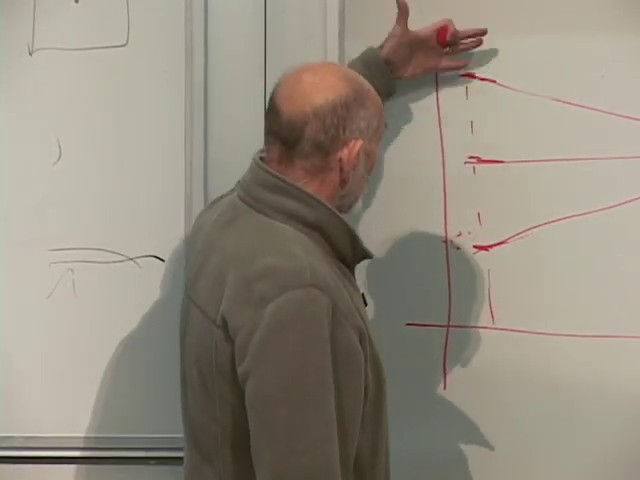
\includegraphics[width=0.70\textwidth]{lecture_05_figure_08.png}
  \caption{示意性的跑动耦合图。三条规范曲线在上升的引力强度变为量级一之前彼此接近。}
  \lectureframe{00:47:18}
  \label{fig:l05-running-couplings-board}
\end{figure}

这是外推，而不是在交叉点处的直接实验。实验室能量与统一能量之间的额外粒子或阈值可以改变斜率。谨慎的结论只是：已知场论在普通距离上没有显示出弦尺度子结构的迹象，而一个合理的弦尺度位于所推断的统一尺度与普朗克尺度之间的巨大区间中的某处。

\begin{classroomqa}
\audiencequestion{正在被外推的是哪三种耦合？\lecturetimestamp{00:48:28}}
\lecturerresponse{它们是与\(U(1)\)、\(SU(2)\)和\(SU(3)\)相关的规范耦合：超荷、弱和强相互作用。电磁作用从电弱混合中涌现，而不是在这一账目中作为一个独立的第四规范因子。}
\end{classroomqa}

\begin{classroomqa}
\audiencequestion{引力常数\(G\)本身会随着我们探测更高能量而增大吗？\lecturetimestamp{00:49:30}}
\lecturerresponse{\(G\)是有量纲的，因此它本身并不是与无量纲规范耦合相比较的正确量。在特征能量\(M\)下，无量纲引力强度示意性地表现为\(GM^2/(\hbar c)\)。该组合随能量增大，并在普朗克尺度处变为量级一。}
\end{classroomqa}

力律使这一比较变得可见：
\begin{equation}
  F_{\mathrm{em}}\sim\frac{e^2}{r^2},
  \qquad
  F_{\mathrm{grav}}\sim\frac{GM^2}{r^2}.
  \label{eq:l05-force-laws}
\end{equation}
因此，\(e^2\)不是与\(G\)比较，而是与自然单位下的\(GM^2\)比较。

\begin{figure}[H]
  \centering
  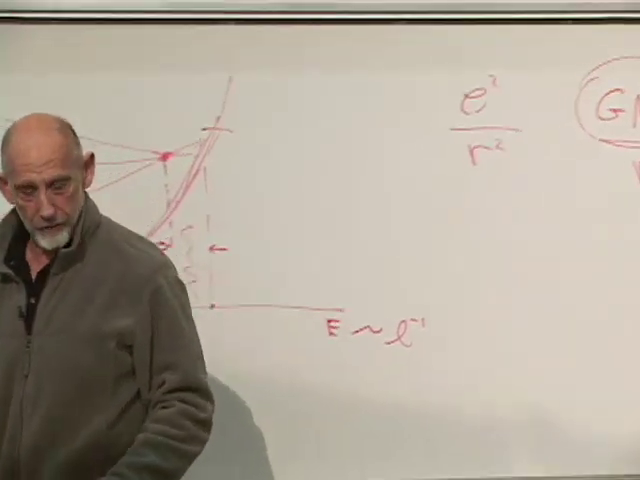
\includegraphics[width=0.74\textwidth]{lecture_05_figure_09.png}
  \caption{用于确定无量纲引力强度的电磁力律与引力力律。}
  \lectureframe{00:50:50}
  \label{fig:l05-force-laws-board}
\end{figure}

\section{为什么直接弦谱学遥不可及}

我们如何通过实验确立电子是一根弦？我们会做强子谱学做过的事：足够猛烈地撞击它，以激发其内部模式，并寻找一个质量遵循弦模式的态塔。如果第一个有质量能级位于\(10^{19}\,\mathrm{GeV}\)附近，那也远超任何直接机器。

总能量并不是唯一的障碍。它还必须被集中在极小的碰撞参数内。这就引出了黑洞。

\begin{classroomqa}
\audiencequestion{在这些能量下，加速器会开始产生小黑洞吗？\lecturetimestamp{00:50:57}}
\lecturerresponse{一旦质心能量被集中在引力半径之内，这就是启发式的预期。恒星黑洞是由引力势能挤压一颗大质量恒星而形成的。微观黑洞则相反，是由动能聚焦到微小碰撞区域而形成的。在四维引力中，所需尺度是普朗克量级。}
\end{classroomqa}

为了提供参照，直线加速器的能量增益大致与其长度成正比。讲座以大约两英里对应大约\(100\,\mathrm{GeV}\)作为简单的SLAC尺度标尺。若以相同梯度达到\(10^{19}\,\mathrm{GeV}\)，长度将乘以大约\(10^{17}\)，从而产生一台星系尺度的机器。

即便这样一台机器也需要光度。束流并不是一次一对地以普朗克长度精度瞄准；而是数量巨大的粒子交叉通过，使得少数粒子在所需碰撞参数下碰撞。将普朗克能量乘以巨大的碰撞率，会产生同样荒谬的功率需求。这些估计是有意粗略的，但其结论是稳定的：在普朗克尺度上进行直接弦谱学并不是一个能够合理设计的实验。

间接证据必须更具结构性：一种能够以足够的具体性给出所观测到的低能粒子与相互作用、从而可被检验的理论，或者紧致化效应在远低于弦尺度的能标下仍然存活。本讲并不声称这样一种决定性的构造已经掌握在手。

\subsection{额外维度与定域化极限}

\begin{classroomqa}
\audiencequestion{额外维度的大小是否也接近普朗克长度？\lecturetimestamp{00:56:23}}
\lecturerresponse{在这一基本图像中，它们预期是极其微小的，尽管这一论证并未将其精确固定。如果某个紧致维度大到足以在较低能量下被探测，那么新的 Kaluza--Klein 模式以及更高维的行为早就应当改变我们所观测到的场论了。因此，该场论的成功外推为这类维度给出了一个上界。}
\end{classroomqa}

\begin{classroomqa}
\audiencequestion{为什么弦或紧致维度不可能比 \(\ell_P\) 小许多个数量级？\lecturetimestamp{00:57:48}}
\lecturerresponse{分辨更短的距离需要更大的动量。超过普朗克尺度之后，定域化所需的能量其引力半径与被探测的区域相当，继而变得比该区域更大。实验在分辨出更小的普通弦之前，就已经制造出了一个黑洞。}
\end{classroomqa}

不确定性原理给出了这一估计。要定域化到 \(\Delta x\)，需要

\begin{classroomqa}
\audiencequestion{一旦选定了普朗克长度与普朗克时间，普朗克质量是如何在物理上被确定的？\lecturetimestamp{00:59:04}}
\lecturerresponse{使用 \(\hbar\) 或 \(G\) 将长度尺度换算为能量。不确定性原理表明，将两个粒子定域化在 \(\ell_P\) 之内需要量级为 \(\hbar/\ell_P\) 的动量，因而需要量级为 \(m_Pc^2\) 的能量。等价地说，它就是使量子长度与引力长度变得相当的那个质量。}
\end{classroomqa}

\begin{equation}
  \Delta p\gtrsim\frac{\hbar}{\Delta x},
  \qquad
  E\sim c\,\Delta p.
  \label{eq:l05-localization}
\end{equation}
在 \(\Delta x=\ell_P\) 处，该能量为
\begin{equation}
  E\sim\frac{\hbar c}{\ell_P}=m_Pc^2.
\end{equation}
与此同时，施瓦西半径
\begin{equation}
  r_s\sim\frac{GE}{c^4}
\end{equation}
在量级上为 \(\ell_P\)，相差若干数值常数。量子定域化与引力坍缩在同一尺度上相遇。

\begin{figure}[H]
  \centering
  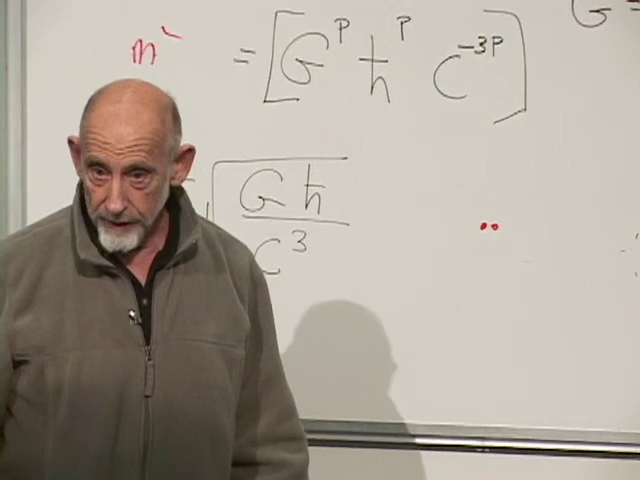
\includegraphics[width=0.74\textwidth]{lecture_05_figure_10.png}
  \caption{在定域化论证过程中重新审视的普朗克长度与质量公式。}
  \lectureframe{01:00:25}
  \label{fig:l05-localization-board}
\end{figure}

至此，尺度设定论证完成。

\section{基态必须位于光子之下}

休息之后有两条可能的方向：开始讲共形变换，或者给出通往临界维数的更古老、更容易的途径。我们选择后者，并附上一句警告。这条容易的论证并不容易，而且它也不是最深刻的理由。尽管如此，它是正确的，并且接近历史上的发现。

回到开弦玻色弦。用横向产生算符作用一次会产生两个极化态。由于不存在纵向的第三个态，该激发必须是一个无质量矢量。在取一个模式-\(1\) 量子使 \(m^2\) 升高一个单位的单位制下，
\begin{equation}
  m_{\mathrm{ground}}^2=-1,
  \qquad
  m_{\mathrm{first}}^2=-1+1=0.
  \label{eq:l05-open-intercept}
\end{equation}
快子基态仍然是玻色弦理论的一个问题；它被承认并暂时搁置。眼下的问题是 \eqref{eq:l05-open-intercept} 中的负单位从何而来。

每个弦模式都是一个谐振子。取 \(\hbar=1\)，其真空能量为
\begin{equation}
  E_{0,n}=\frac{\omega_n}{2}.
\end{equation}
对于弦，\(\omega_n=n\)，因此一个横向坐标形式上贡献
\begin{equation}
  E_0^{(1)}
  =\frac12\sum_{n=1}^{\infty}n.
  \label{eq:l05-formal-zero-point}
\end{equation}

\begin{figure}[H]
  \centering
  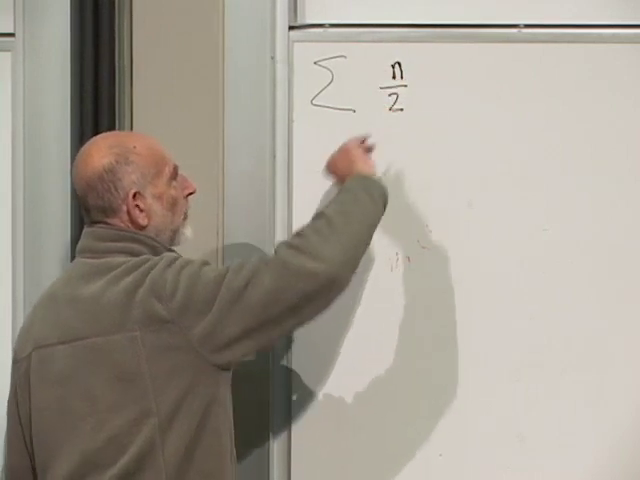
\includegraphics[width=0.70\textwidth]{lecture_05_figure_11.png}
  \caption{在回顾了模式频率之后写出的零点求和 \(\sum n/2\)。}
  \lectureframe{01:06:18}
  \label{fig:l05-zero-point-board}
\end{figure}

现在困难变得尖锐了。
\eqref{eq:l05-formal-zero-point} 中的每一项都是正的，而且该求和发散。它如何能给出一个有限的负截距？

\section{在读取谱之前先减去运动}

在对该求和进行正规化之前，回顾一下为什么内能会被等同于质量平方。对于一个携带大纵向动量 \(P>0\) 的粒子，
\begin{equation}
  E=\sqrt{P^2+m^2}
   =P+\frac{m^2}{2P}
   +O(P^{-3}).
  \label{eq:l05-large-p-energy}
\end{equation}

\begin{figure}[H]
  \centering
  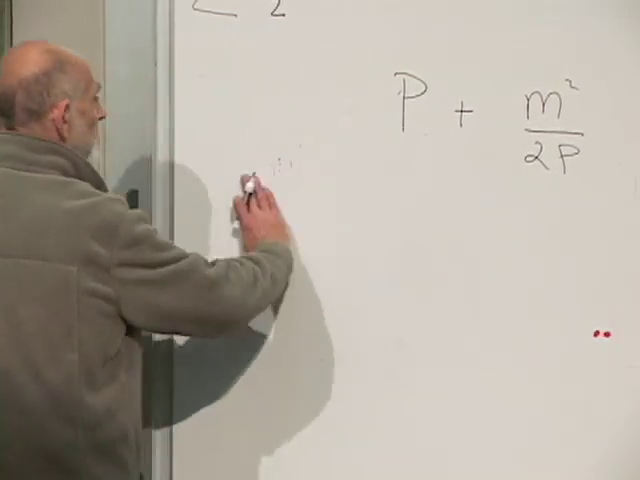
\includegraphics[width=0.70\textwidth]{lecture_05_figure_12.png}
  \caption{将整体动量与内部质量项分离开来的大-\(P\) 展开。}
  \lectureframe{01:07:35}
  \label{fig:l05-fast-energy-board}
\end{figure}

第一项是沿 \(z\) 轴的无趣的整体运动。它是守恒的，并且对于所有具有相同 \(P\) 的内部态都是共同的。减去它并重新标度，就消去了运动学上的时间膨胀：
\begin{equation}
  \begin{aligned}
    E-P&=\frac{m^2}{2P}+O(P^{-3}),\\
    2P(E-P)&=m^2+O(P^{-2}).
  \end{aligned}
  \label{eq:l05-internal-energy}
\end{equation}

原子提供了物理图像。对氢原子进行助推。它的总能量增大，但两个内部能级之间的能量差，按实验室时间测量，却缩小了，因为原子的时钟发生了膨胀。\eqref{eq:l05-large-p-energy} 中的因子 \(1/P\) 就是这种压低。乘以 \(2P\) 便恢复了不变的质量平方差。

因此，裸基态能量不必字面上就是 \(-1\)。它可能包含一个与整体纵向能量相关的大块状态无关部分，再加上一个有限的内禀剩余部分。讲义重写了助推后的关系式，以展示这两部分，然后才转回振子求和。

\begin{figure}[H]
  \centering
  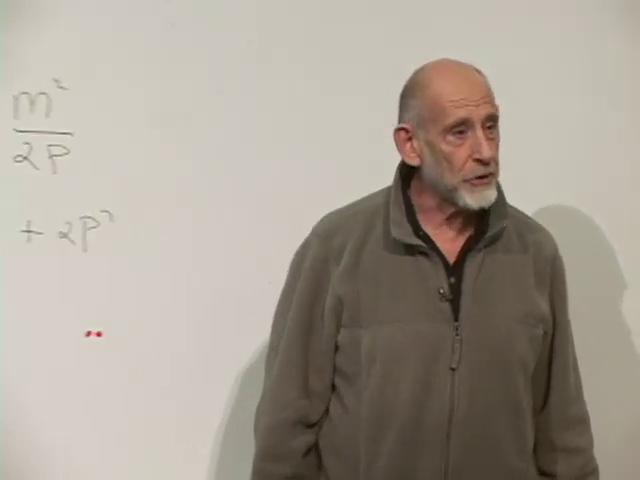
\includegraphics[width=0.76\textwidth]{lecture_05_figure_13.png}
  \caption{与大的状态无关纵向贡献并列展示的不变质量项。}
  \lectureframe{01:11:34}
  \label{fig:l05-infinite-piece-board}
\end{figure}

无穷大的真空能量在量子场论中是熟悉的。人们常常把一个发散的状态无关常数与可观测的能量差分开。讲义将此与房间中电磁场的零点能相比较，并坦率地称这一做法不能令人满意，但却是标准的。这里我们遵循同样的启发式做法：分离出发散部分，并追问是否留下一个确定的有限剩余。

\section{对求和进行正规化}

引入一个正的正规化因子 \(\epsilon\)：
\begin{equation}
  S_1(\epsilon)
  =\sum_{n=1}^{\infty}n e^{-n\epsilon}.
  \label{eq:l05-regulated-sum}
\end{equation}
对每个 \(\epsilon>0\)，指数最终会压倒因子 \(n\)，因此该求和收敛。让 \(\epsilon\) 趋于零便去掉了截断。

\begin{figure}[H]
  \centering
  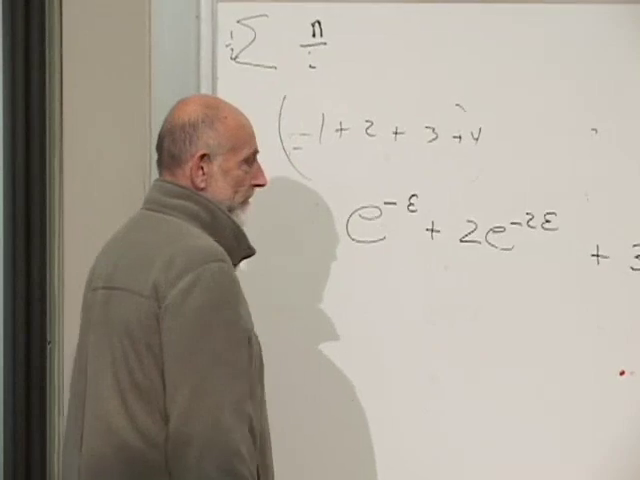
\includegraphics[width=0.78\textwidth]{lecture_05_figure_14.png}
  \caption{逐项施加于 \(1+2+3+\cdots\) 的指数正规化因子。}
  \lectureframe{01:16:42}
  \label{fig:l05-regulator-board}
\end{figure}

因子 \(n\) 可以通过微分生成：
\begin{equation}
  S_1(\epsilon)
  =
  -\frac{d}{d\epsilon}
  \sum_{n=1}^{\infty}e^{-n\epsilon}.
  \label{eq:l05-derivative-trick}
\end{equation}

\begin{figure}[H]
  \centering
  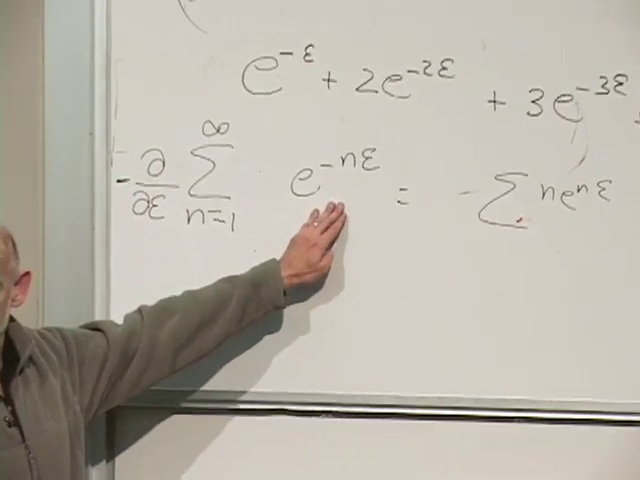
\includegraphics[width=0.76\textwidth]{lecture_05_figure_15.png}
  \caption{对截断参数求导会带下 \(-n\)。}
  \lectureframe{01:18:05}
  \label{fig:l05-derivative-board}
\end{figure}

剩下的级数是几何级数：
\begin{equation}
  S_0(\epsilon)
  \equiv
  \sum_{n=1}^{\infty}e^{-n\epsilon}
  =
  \frac{e^{-\epsilon}}{1-e^{-\epsilon}}
  =
  \frac{1}{e^\epsilon-1}.
  \label{eq:l05-geometric-sum}
\end{equation}

\begin{figure}[H]
  \centering
  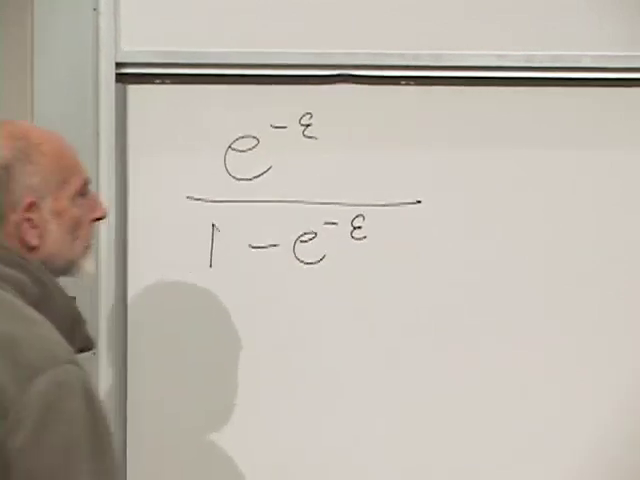
\includegraphics[width=0.68\textwidth]{lecture_05_figure_16.png}
  \caption{正规化后的几何级数的闭式形式。}
  \lectureframe{01:19:12}
  \label{fig:l05-geometric-board}
\end{figure}

在小的 \(\epsilon\) 处展开：
\begin{equation}
  S_0(\epsilon)
  =
  \frac{1}{\epsilon}
  -\frac12
  +\frac{\epsilon}{12}
  -\frac{\epsilon^3}{720}
  +O(\epsilon^5).
  \label{eq:l05-bernoulli-expansion}
\end{equation}
板书是通过分别展开分子和分母、提出一个 \(\epsilon\) 的幂、然后展开倒数而得到这一结果的。该计算包含若干课堂上的符号检查；紧凑表达式 \eqref{eq:l05-bernoulli-expansion} 是其整理后的结果。

\begin{figure}[H]
  \centering
  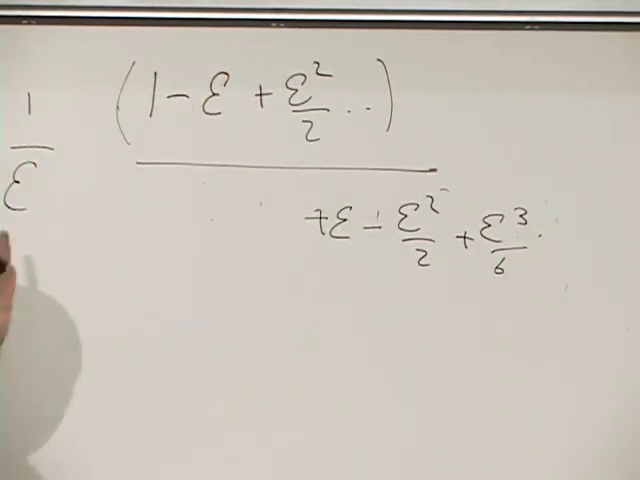
\includegraphics[width=0.78\textwidth]{lecture_05_figure_17.png}
  \caption{在简化倒数之前的分子和分母展开。}
  \lectureframe{01:23:10}
  \label{fig:l05-expansion-board}
\end{figure}

施加 \(-d/d\epsilon\) 得到
\begin{equation}
  S_1(\epsilon)
  =
  \frac{1}{\epsilon^2}
  -\frac{1}{12}
  +\frac{\epsilon^2}{240}
  +O(\epsilon^4).
  \label{eq:l05-regulated-result}
\end{equation}

\begin{figure}[H]
  \centering
  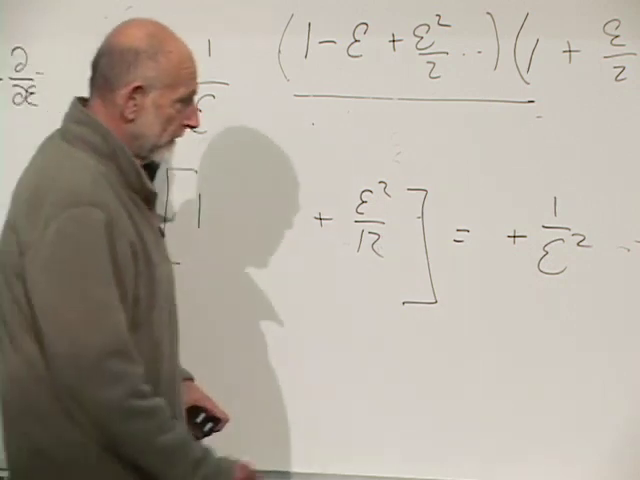
\includegraphics[width=0.78\textwidth]{lecture_05_figure_18.png}
  \caption{正规化计算末尾的发散 \(1/\epsilon^2\) 项和有限 \(-1/12\) 剩余。}
  \lectureframe{01:29:48}
  \label{fig:l05-minus-twelve-board}
\end{figure}

人们常开玩笑地把这一结果概括为
\(1+2+3+\cdots=-1/12\)。这并不是通常意义下的收敛。方程
\eqref{eq:l05-regulated-result} 表明，这个特定的正规化因子产生一个发散项加上一个与正规化因子无关的有限部分：
\begin{equation}
  \underbrace{\frac{1}{\epsilon^2}}_{\text{divergent}}
  \;+\;
  \underbrace{\left(-\frac{1}{12}\right)}_{\text{finite}}
  \;+\;O(\epsilon^2).
\end{equation}
讲义把第一项吸收进已经存在的状态无关部分，并保留第二项。它还保留了归因于泡利的警告：无穷大本身并不使一个量成为零。一个自洽的理论必须解释为什么允许做这种减法。

在
\eqref{eq:l05-formal-zero-point} 中恢复二分之一这个因子，一个横向坐标贡献
\begin{equation}
  E_0^{(1)}=-\frac{1}{24}.
  \label{eq:l05-one-transverse-zero-point}
\end{equation}

\begin{figure}[H]
  \centering
  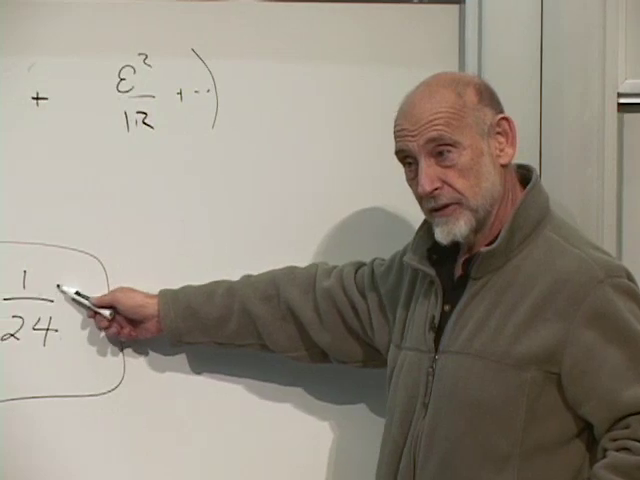
\includegraphics[width=0.68\textwidth]{lecture_05_figure_19.png}
  \caption{二分之一这个因子把有限的
  \(-1/12\) 转换为每个横向坐标的 \(-1/24\)。}
  \lectureframe{01:33:42}
  \label{fig:l05-minus-twenty-four-board}
\end{figure}

\section{数横向方向}

设 \(D_\perp\) 为横向弦坐标的数目。它们的总真空贡献为
\begin{equation}
  E_0^{\mathrm{open}}
  =-\frac{D_\perp}{24}.
  \label{eq:l05-open-vacuum}
\end{equation}
为了使第一个开弦振子把基态从
\(-1\) 提升到无质量能级，我们需要
\begin{equation}
  -\frac{D_\perp}{24}=-1.
\end{equation}
因此
\begin{equation}
  D_\perp=24.
\end{equation}
这些就是垂直于大纵向动量的方向。加上那个纵向空间方向和时间，得到
\begin{equation}
  D=D_\perp+2=26.
  \label{eq:l05-critical-dimension}
\end{equation}

\begin{classroomqa}
\audiencequestion{这个论证是何时进入弦理论的？\lecturetimestamp{01:35:27}}
\lecturerresponse{它属于最初强子弦的时代，大约在
1969 年和 1970 年代初。雷吉轨迹当时已在实验上为人所知。一旦振子模型被独立地探索，人们就发现第一激发态具有两个而非三个矢量极化，从而迫使它无质量。所需的截距随即迅速导致二十四个横向振子。}
\end{classroomqa}

在当时，这看起来几乎奇怪得令人难以置信。一个正规化后的真空求和为什么应当知道时空的维度？然而各个部分彼此吻合：无质量矢量、截距和横向振子数目都选出了同一个数。

\subsection{闭弦检验这个计数}

一根闭弦需要一个左行模式和一个右行模式才能达到它的第一个物理无质量能级。因此它的基态必须从零以下两个单位开始。

\begin{classroomqa}
\audiencequestion{如果二十四个横向方向只给出\(-1\)，那么闭弦是否必须生活在四十八个横向方向中？\lecturetimestamp{01:37:47}}
\lecturerresponse{不。同一个时空中同时包含开弦和闭弦。闭弦已经具有两倍的振子内容：在每个世界面方向上各有一个振子塔在循环。每个塔贡献\(-24/24=-1\)，因此两者合起来给出\(-2\)。}
\end{classroomqa}

因此
\begin{equation}
  E_0^{\mathrm{closed}}
  =
  2\left(-\frac{D_\perp}{24}\right)
  =-2
  \qquad (D_\perp=24).
\end{equation}
从每个扇区各添加一个振子会使态升高两个单位，并落在零质量平方处，这正是前一讲中引力子多重态出现的位置。

这一吻合使论证显得更合理，但它仍然不是深层的解释。在现代量子化中，正规序常数、洛伦兹代数或Virasoro代数的封闭性，以及共形反常的抵消，都属于同一个自洽结构。该结构同时确定了截距和临界维数；有限截断的剩余项只是通向它的历史途径。
\editorialnote{调节子计算是正规序常数的一种启发式看法。\(D=26\)的更深入推导需要世界面共形不变性，等价地需要共形反常的抵消和约束代数的自洽性。}

接下来就是那条更深入的路线。开始只需要少量复分析：复坐标、解析函数以及Cauchy--Riemann方程。所承诺的物理图像是土耳其软糖---，朝一个方向拉，朝另一个方向抻，在不破坏关键结构的情况下重塑形状。这一图像背后的数学就是共形不变性。

\chapter{散射、对偶性与Veneziano振幅}

\lectureoverview{散射将碰撞约化为可与实验比较的不变量数据。对于四个全同粒子，这些数据可以组织为Mandelstam变量\(s,t,u\)，其中只有两个是独立的。普通的粒子交换于是提示存在分离的直接道与交叉道。Veneziano振幅推翻了这一预期：一个函数同时包含两种道的描述。本讲的后半部分从两条开弦出发构造该函数：它们相接、作为一个振荡链演化，然后再次分裂。}

\section{理论必须预言什么}

费米弦解决了纯玻色模型的两个缺陷：它们允许费米子态，并且在适当的投影之后消除快子。它们的临界时空维数是十而不是二十六。因此额外维度仍然存在，但其紧致化被推迟。当前的主题是散射。
\editorialnote{无快子的陈述指的是在所需投影之后自洽的超弦谱；仅仅加入世界面费米子本身并不足够。}

散射未必是粒子所做的最有趣的事情。它只是实验能够干净地重复的操作。将指定的粒子相互射向对方，记录从碰撞中出射的粒子，并推断隐藏在相互作用区域内部的动力学。当一个理论给出复振幅
\begin{equation}
  \mathcal A(\hbox{incoming data}\to\hbox{outgoing data}),
\end{equation}
时，它才成为定量的；该振幅的模平方与通常的相空间因子一起给出该结果的概率。

\begin{figure}[H]
  \centering
  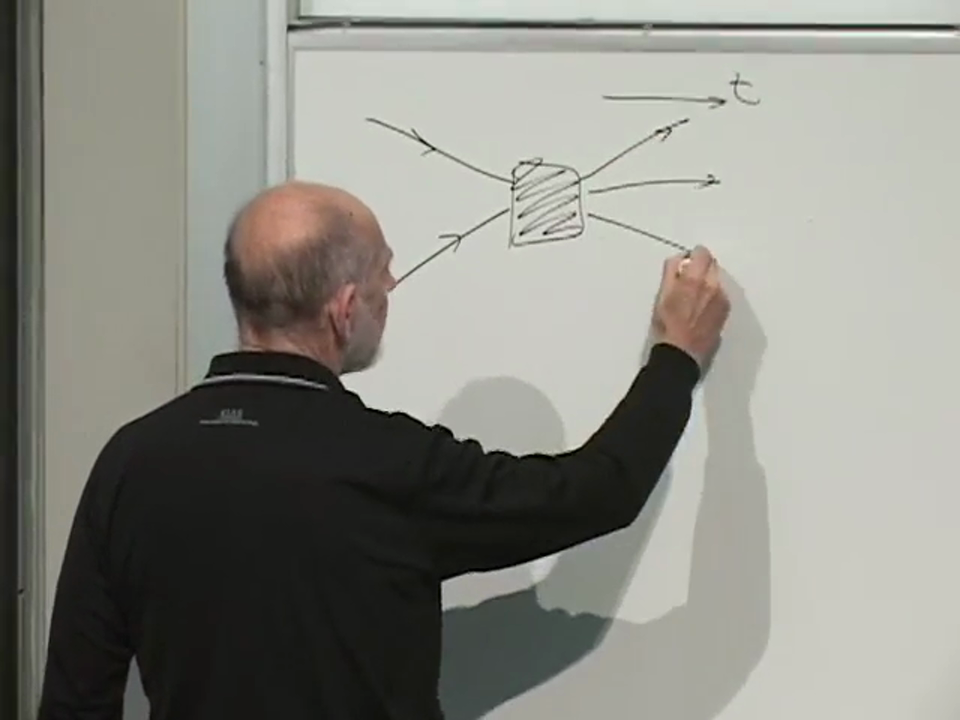
\includegraphics[width=0.72\textwidth]{lecture_06_figure_01.png}
  \caption{入射粒子进入黑箱相互作用区域，出射粒子从中射出；时间水平绘制。}
  \lectureframe{00:02:35}
  \label{fig:l06-black-box}
\end{figure}

粒子还带有自旋、电荷和种类标签。为了首先揭示运动学，让我们暂时抑制除动量以外的一切。

\section{四动量与全入射约定}

将一个粒子的四动量写为
\begin{equation}
  k^\mu=(k^0,\mathbf k)=(E,\mathbf p).
\end{equation}
本讲使用mostly-plus度规，因此
\begin{equation}
  k^2\equiv \mathbf p^2-E^2.
\end{equation}
相对论色散关系因此为
\begin{equation}
  E^2-\mathbf p^2=m^2,
  \qquad
  k^2=-m^2.
  \label{eq:l06-mass-shell}
\end{equation}
改变空间动量会改变能量，但不会使粒子离开其质量壳。

\begin{figure}[H]
  \centering
  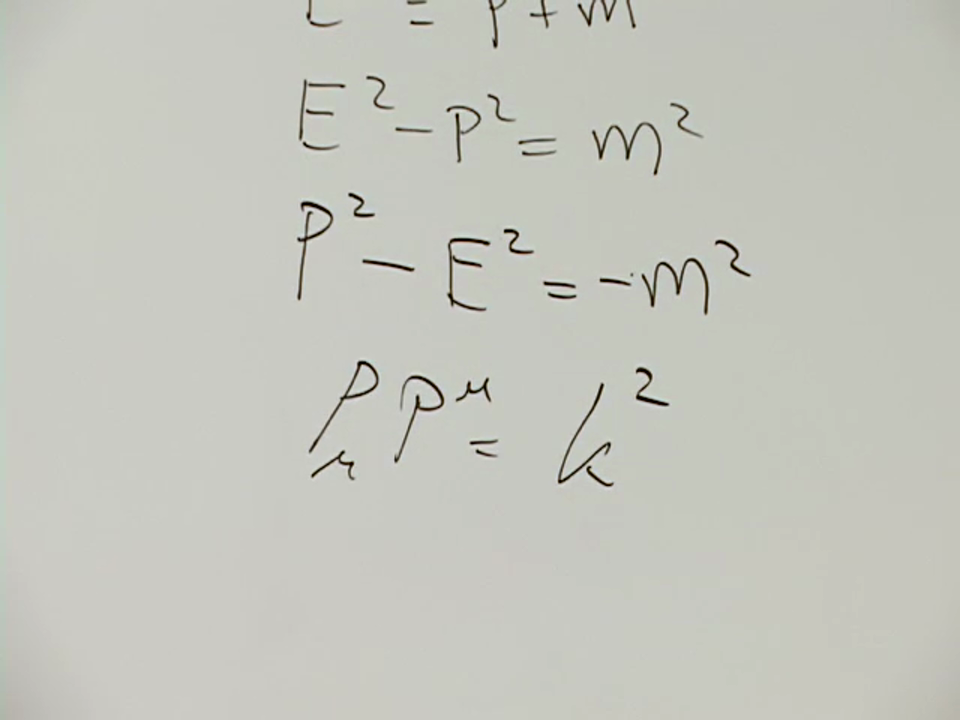
\includegraphics[width=0.66\textwidth]{lecture_06_figure_02.png}
  \caption{本讲通篇所用度规约定下的质量壳条件。}
  \lectureframe{00:05:56}
  \label{fig:l06-mass-shell}
\end{figure}

考虑两个粒子以动量\(k_1,k_2\)入射，两个粒子以物理动量\(q_3,q_4\)出射。能量与动量守恒是一个四矢量方程，
\begin{equation}
  k_1+k_2=q_3+q_4.
  \label{eq:l06-physical-conservation}
\end{equation}
方便的做法是为每条外线指定一个入射动量：
\begin{equation}
  k_3\equiv-q_3,
  \qquad
  k_4\equiv-q_4.
\end{equation}
于是
\begin{equation}
  k_1+k_2+k_3+k_4=0,
  \label{eq:l06-all-incoming}
\end{equation}
并且每条腿都满足\(k_i^2=-m_i^2\)。出射粒子只有在这种记账约定下才具有负能量；它们的物理能量仍然为正。

\begin{figure}[H]
  \centering
  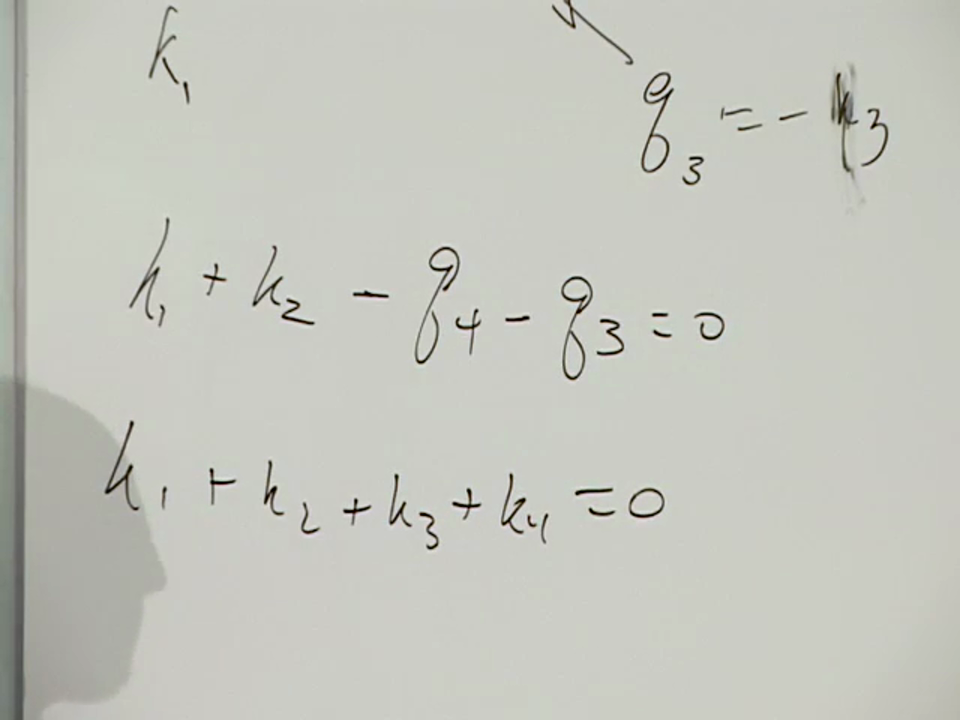
\includegraphics[width=0.68\textwidth]{lecture_06_figure_03.png}
  \caption{物理出射动量被反向，以便所有四个外部动量都可以对称地当作入射来处理。}
  \lectureframe{00:09:10}
  \label{fig:l06-all-incoming-board}
\end{figure}

起初振幅看起来是十六个分量的函数，
\(\mathcal A(k_1,k_2,k_3,k_4)\)。其中大多数是冗余的。转到质心系，将入射动量旋转到选定的轴上，并为了简单起见假设四个粒子质量相同。入射态于是由一个数固定，即质心能量。出射空间动量必须大小相等、方向相反，并且其大小与入射粒子对相同。只剩下它们的偏转角\(\theta\)。因此该过程有两个独立的运动学变量：
\begin{equation}
  E_{\mathrm{cm}},
  \qquad
  \theta.
  \label{eq:l06-two-data}
\end{equation}

\section{Mandelstam变量}

\eqref{eq:l06-two-data}中的两个物理量应当能够不选择参考系地表达。采用全入射约定，定义
\begin{equation}
  \begin{aligned}
    -s&=(k_1+k_2)^2,\\
    -t&=(k_1+k_3)^2,\\
    -u&=(k_1+k_4)^2.
  \end{aligned}
  \label{eq:l06-mandelstam}
\end{equation}
在质心系中，\(k_1+k_2\)的空间部分相消，因此
\begin{equation}
  s=E_{\mathrm{cm}}^2.
  \label{eq:l06-s-energy}
\end{equation}

对于出射物理动量\(q_3=-k_3\)，
\begin{equation}
  k_1+k_3=k_1-q_3
\end{equation}
是从腿1转移到腿3的动量。对于相等的外部质量，设入射空间动量大小为\(p\)，
\begin{equation}
  -t=2p^2(1-\cos\theta),
  \qquad
  -u=2p^2(1+\cos\theta).
  \label{eq:l06-tu-angle}
\end{equation}
因此\(t\)和\(u\)携带探测器所测量的角度信息。

\begin{figure}[H]
  \centering
  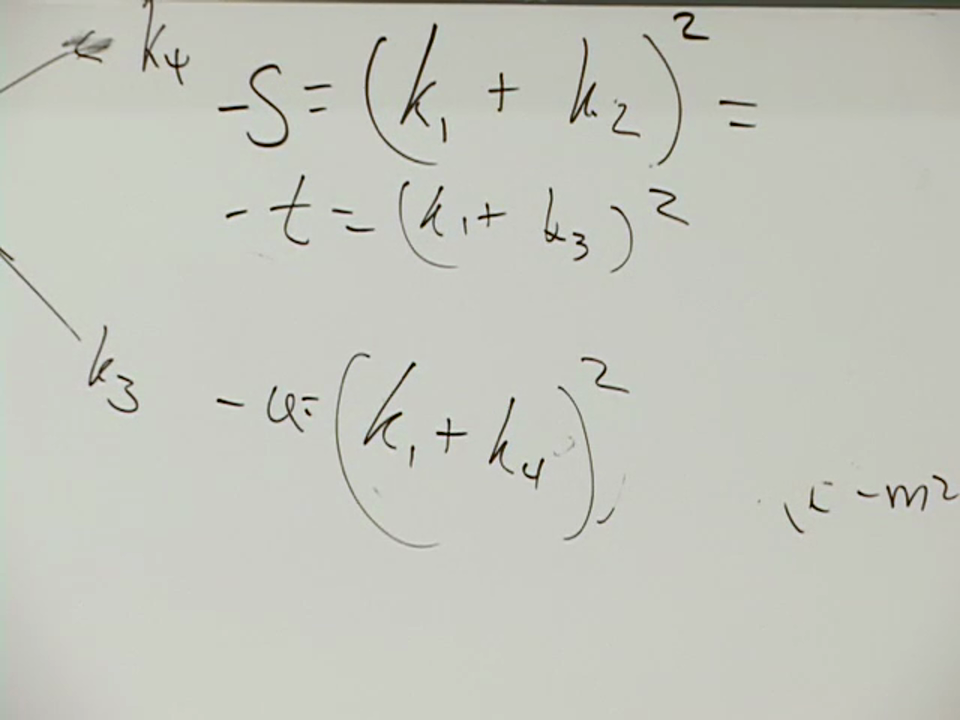
\includegraphics[width=0.74\textwidth]{lecture_06_figure_04.png}
  \caption{全入射约定下\(s,t,u\)的对称定义。}
  \lectureframe{00:26:20}
  \label{fig:l06-stu-board}
\end{figure}

三个符号并不意味着三个独立的数据。将
\eqref{eq:l06-all-incoming}平方并利用\(k_i^2=-m^2\)，对于相等质量给出
\begin{equation}
  s+t+u=4m^2
  \label{eq:l06-stu-constraint}
\end{equation}
一旦\(s\)和\(t\)已知，\(u\)就被固定。

\begin{classroomqa}
\audiencequestion{真空能否像摩擦那样使自由运动的粒子减速？\lecturetimestamp{00:27:17}}
\lecturerresponse{在平移不变的真空里不能。缺失的动量无处可去，因此动量守恒禁止这种摩擦。人们可以设想一种介质或一种不同的真空，它选定了一个优先的静止参考系，但那不是这里所使用的真空。}
\end{classroomqa}

\begin{classroomqa}
\audiencequestion{为什么两个出射粒子必须具有相等的能量？\lecturetimestamp{00:27:54}}
\lecturerresponse{在质心系中，它们的空间动量必须大小相等、方向相反。对于所讨论的等质量过程，相等的动量大小通过\(E^2=p^2+m^2\)给出相等的能量。如果出射粒子的质量不同，那么最后这个结论就必须修改。}
\end{classroomqa}

\section{直接道与交叉道}

一个简单的点粒子图让粒子1和2形成一个质量为\(M\)的中间粒子，该粒子随后衰变为3和4。忽略分子因子和极点规定，其特征依赖关系为
\begin{equation}
  \mathcal A_s\sim\frac{g^2}{s-M^2}.
  \label{eq:l06-s-channel}
\end{equation}
这就是直接过程，或称\(s\)道过程。把连接方式侧转过来，就得到两条外线之间的交换，
\begin{equation}
  \mathcal A_t\sim\frac{g^2}{t-M^2},
  \label{eq:l06-t-channel}
\end{equation}
即交叉过程，或称\(t\)道过程。第三种连接方式给出
\begin{equation}
  \mathcal A_u\sim\frac{g^2}{u-M^2}.
  \label{eq:l06-u-channel}
\end{equation}

\begin{figure}[H]
  \centering
  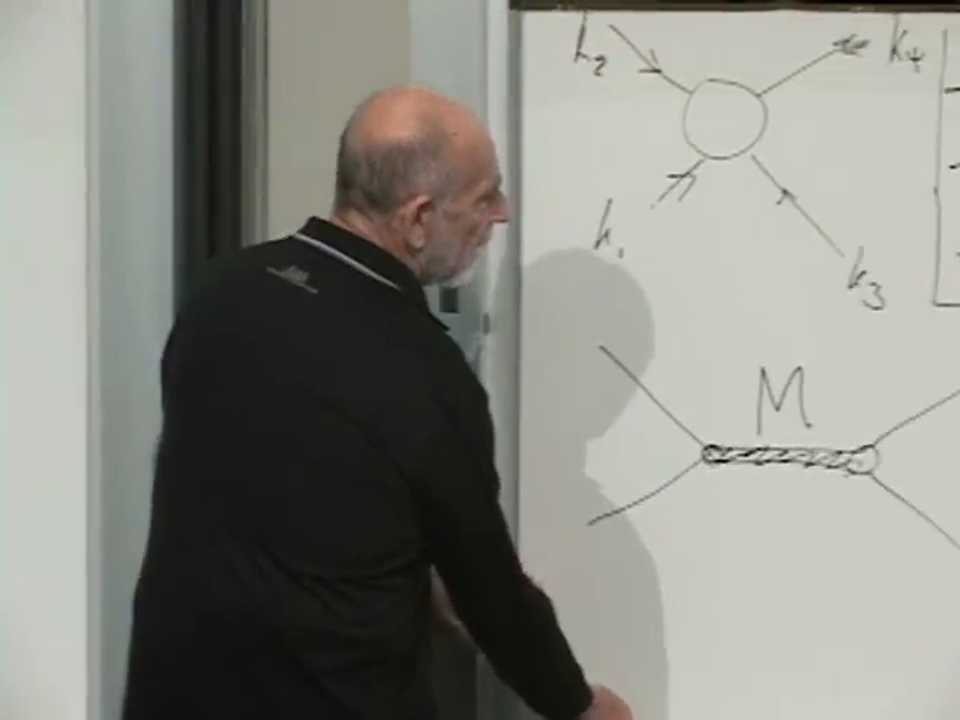
\includegraphics[width=0.72\textwidth]{lecture_06_figure_05.png}
  \caption{通过中间态的直接产生以及相应的极点\(g^2/(s-M^2)\)；交叉连接方式正在同一块黑板上拼装。}
  \lectureframe{00:30:50}
  \label{fig:l06-channel-board}
\end{figure}

这一区别是物理上的。在这个粗糙的标量层面上，\eqref{eq:l06-s-channel}依赖于碰撞能量，但不依赖于角度。复合态在衰变之前已经忘记了入射方向，因此它的衰变是各向同性的。交换振幅依赖于动量转移，因而依赖于角度；轻的交换粒子强烈倾向于小偏转。自旋会带来进一步的角度依赖，但极点结构已经可见。

\begin{classroomqa}
\audiencequestion{缺失的\(u\)道是否产生第三项？\lecturetimestamp{00:34:47}}
\lecturerresponse{是的，只要粒子身份和耦合允许这种连接方式。于是人们就纳入一个在\(u=M^2\)处有极点的项。它不是一个新的独立运动学变量，因为\(s+t+u=4m^2\)，但它是一个不同的道图。}
\end{classroomqa}

\section{一个函数，两种道描述}

单个极点作为介子散射的模型是很差的。两个介子可以形成许多共振态，具有一系列质量和角动量。1960年代的第一反应是添加更多的\(s\)道极点、更多的\(t\)道极点，以及允许的\(u\)道极点。随后人们发现了一个经济得多的函数。在讲座的单位制中，线性雷吉轨迹及其截距已被吸收进\(s\)和\(t\)，该函数为
\begin{equation}
  \mathcal A_{\mathrm V}(s,t)
  \propto
  \frac{\Gamma(-s)\Gamma(-t)}{\Gamma(-s-t)}.
  \label{eq:l06-veneziano}
\end{equation}
伽马函数延拓了阶乘：
\begin{equation}
  \Gamma(n)=(n-1)!
\end{equation}
在正整数处成立。

\begin{figure}[H]
  \centering
  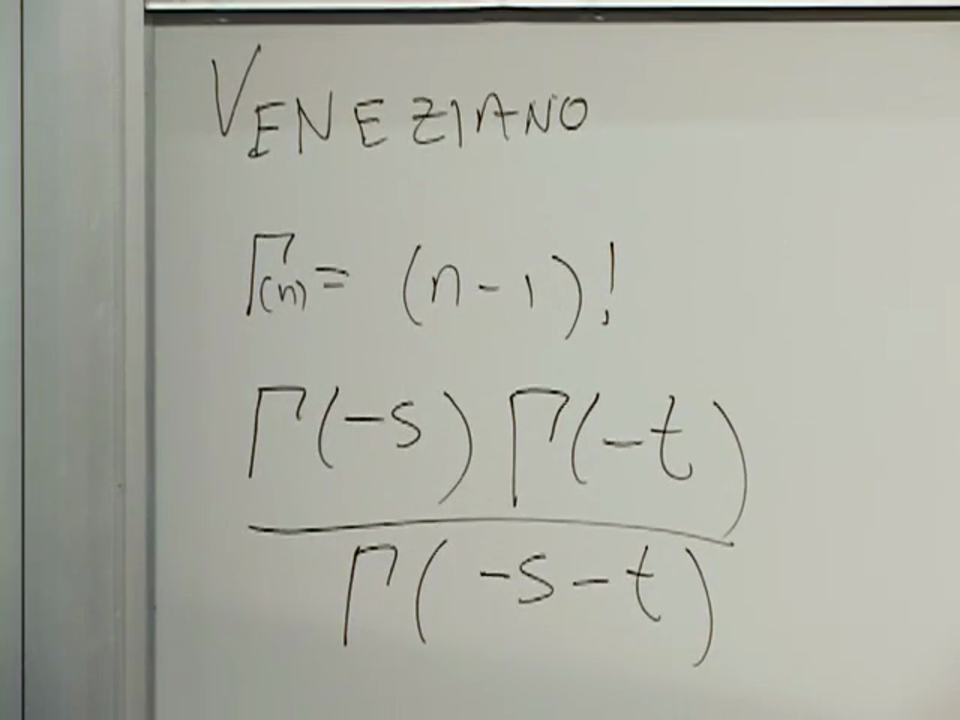
\includegraphics[width=0.68\textwidth]{lecture_06_figure_06.png}
  \caption{写成伽马函数对称比值的韦内齐亚诺振幅。}
  \lectureframe{00:42:25}
  \label{fig:l06-veneziano-board}
\end{figure}

\(\Gamma(-s)\)的极点再现了直接道共振态的无限序列。然而同一个表达式在\(s\leftrightarrow
t\)下是对称的，因此它的\(\Gamma(-t)\)极点给出交叉道展开。这些并不是两个分别添加的贡献。一个解析函数容许两种描述。这就是直接道共振态与交叉道交换之间对偶性的旧观念。

\begin{classroomqa}
\audiencequestion{一个振幅如何能在不把它们相加的情况下同时包含两个道的求和？\lecturetimestamp{00:43:32}}
\lecturerresponse{这正是令人惊讶之处。在\(s\)道极点附近展开该函数，就把它组织为直接共振态；在\(t\)道极点附近展开该函数，就把同一个函数组织为交换。要解释为什么这两种读法是同一回事，需要一个微观模型，而这个模型就是相互作用弦。}
\end{classroomqa}

\section{开弦扫出的一条带}

用下式参数化一条开弦：
\begin{equation}
  0\leq\sigma\leq\pi.
\end{equation}
标记\(\sigma\)不是时空位置。嵌入\(X^\mu(\sigma,\tau)\)告诉我们那个带标记的点位于时空中的何处，而\(\tau\)度量演化。点粒子扫出一条世界线；运动的弦扫出一个二维世界面。在自由理论中，每个嵌入坐标满足
\begin{equation}
  \frac{\partial^2X^\mu}{\partial\tau^2}
  -
  \frac{\partial^2X^\mu}{\partial\sigma^2}
  =0.
  \label{eq:l06-wave-equation}
\end{equation}

\begin{figure}[H]
  \centering
  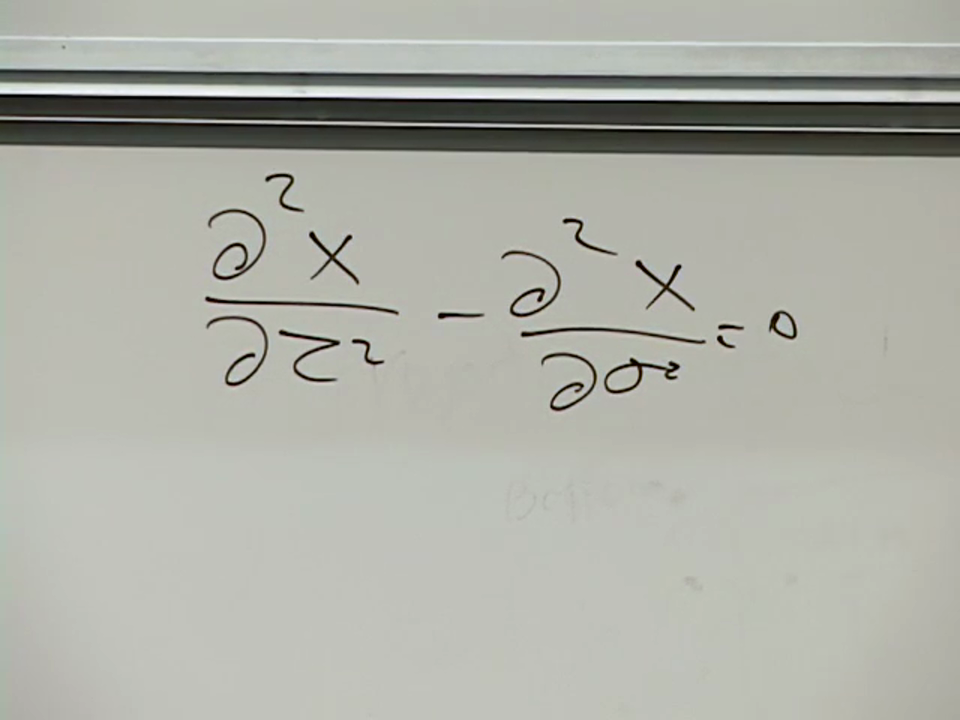
\includegraphics[width=0.70\textwidth]{lecture_06_figure_07.png}
  \caption{支配世界面带上的每个自由弦坐标的波动方程。}
  \lectureframe{00:49:10}
  \label{fig:l06-wave-equation-board}
\end{figure}

对于散射构造而言，不宜过早取连续极限。将每根弦替换为\(n\)个由弹簧连接的质量点。世界面于是成为邻近世界线的一个稠密集合，其简正模就是普通的谐振子。两条入射链可以在其端点处接触。在该事件处，一根新弹簧将它们连接起来，它们作为一根更长的链演化一段时间\(\tau\)，随后一根弹簧断裂，于是两条出射链出现。

\begin{figure}[H]
  \centering
  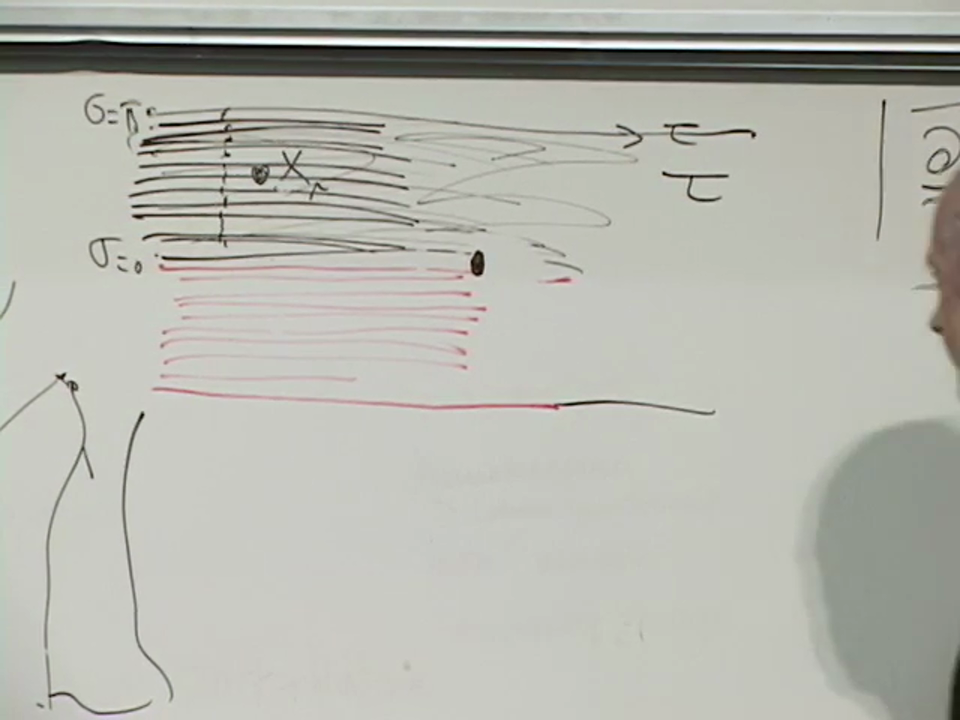
\includegraphics[width=0.72\textwidth]{lecture_06_figure_08.png}
  \medskip

  \begin{tikzpicture}[x=0.85cm,y=0.70cm]
    \draw[thick] (0,2.2) -- (2.1,2.2) -- (3.1,1.5);
    \draw[thick] (0,0.8) -- (2.1,0.8) -- (3.1,1.5);
    \draw[thick] (3.1,1.5) -- (5.5,1.5);
    \draw[thick] (5.5,1.5) -- (6.5,2.2) -- (8.6,2.2);
    \draw[thick] (5.5,1.5) -- (6.5,0.8) -- (8.6,0.8);
    \draw[<->] (3.1,0.35) -- node[below] {\(\tau\)} (5.5,0.35);
    \node[left] at (0,2.2) {1};
    \node[left] at (0,0.8) {2};
    \node[right] at (8.6,2.2) {3};
    \node[right] at (8.6,0.8) {4};
  \end{tikzpicture}
  \caption{两条离散化的开弦接触，形成一根中间弦并持续一段时间\(\tau\)，然后分裂。源帧保留了弹簧与世界线的构造；示意图则将其连通性单独抽出。}
  \lectureframe{00:51:25}
  \label{fig:l06-string-joining}
\end{figure}

这两根弦只是在参数空间中被画成相邻。它们的时空位置不必相邻，直到端点坐标真正重合为止。重参数化自由度使得连接与分裂事件可以被放置在图上方便的位置；这一几何自由度将在下一讲中成为共形对称性。

\section{慢动作中的振子计算}

设第一条链的坐标为\(x_1,\ldots,x_n\)，第二条链的坐标为\(x_{n+1},\ldots,x_{2n}\)。它们的质心坐标为
\begin{equation}
  X_{\mathrm{cm}}^{(1)}
  =\frac1n\sum_{a=1}^{n}x_a,
  \qquad
  X_{\mathrm{cm}}^{(2)}
  =\frac1n\sum_{a=n+1}^{2n}x_a.
  \label{eq:l06-chain-centers}
\end{equation}
具有确定动量\(k_1\)的链，其波函数为质心平面波乘以内部振子基态：
\begin{align}
  \Psi_1
  &=
  e^{ik_1\cdot X_{\mathrm{cm}}^{(1)}}
  \psi_0(x_1,\ldots,x_n),
  \\
  \Psi_2
  &=
  e^{ik_2\cdot X_{\mathrm{cm}}^{(2)}}
  \psi_0(x_{n+1},\ldots,x_{2n}).
  \label{eq:l06-two-wavefunctions}
\end{align}
因子\(\psi_0\)依赖于相对坐标，而不依赖于整条链的共同平移。由于入射弦最初是彼此分离的量子系统，
\begin{equation}
  \Psi_{\mathrm{in}}=\Psi_1\Psi_2.
  \label{eq:l06-product-state}
\end{equation}

\begin{figure}[H]
  \centering
  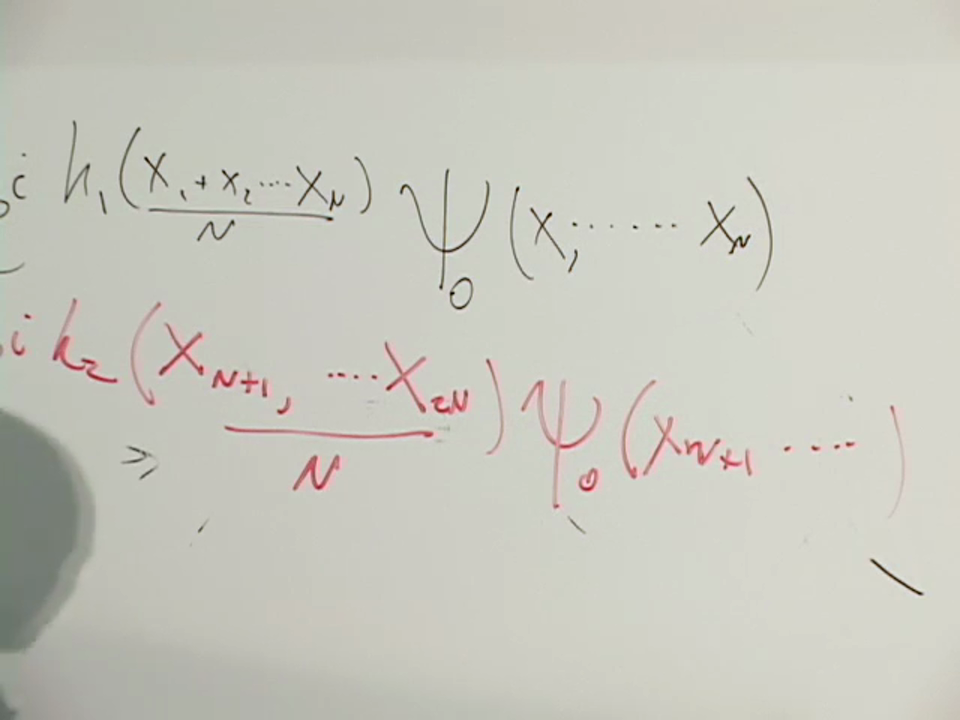
\includegraphics[width=0.76\textwidth]{lecture_06_figure_09.png}
  \caption{两个动量平面波及其内部振子基态因子，以不同颜色写出。}
  \lectureframe{00:58:05}
  \label{fig:l06-wavefunctions-board}
\end{figure}

连接操作选出该波函数中两个端点坐标相一致的部分：
\begin{equation}
  x_n=x_{n+1}.
  \label{eq:l06-endpoint-contact}
\end{equation}
在该瞬间，其余坐标保持不变。随后，所选出的态用单根更长链的哈密顿量\(H_{\mathrm{joined}}\)演化：
\begin{equation}
  \Psi(\tau)
  =
  e^{-iH_{\mathrm{joined}}\tau}\Psi(0).
  \label{eq:l06-time-evolution}
\end{equation}
最后，取它与携带动量\(q_3,q_4\)的出射弦态之积的重叠。

\begin{figure}[H]
  \centering
  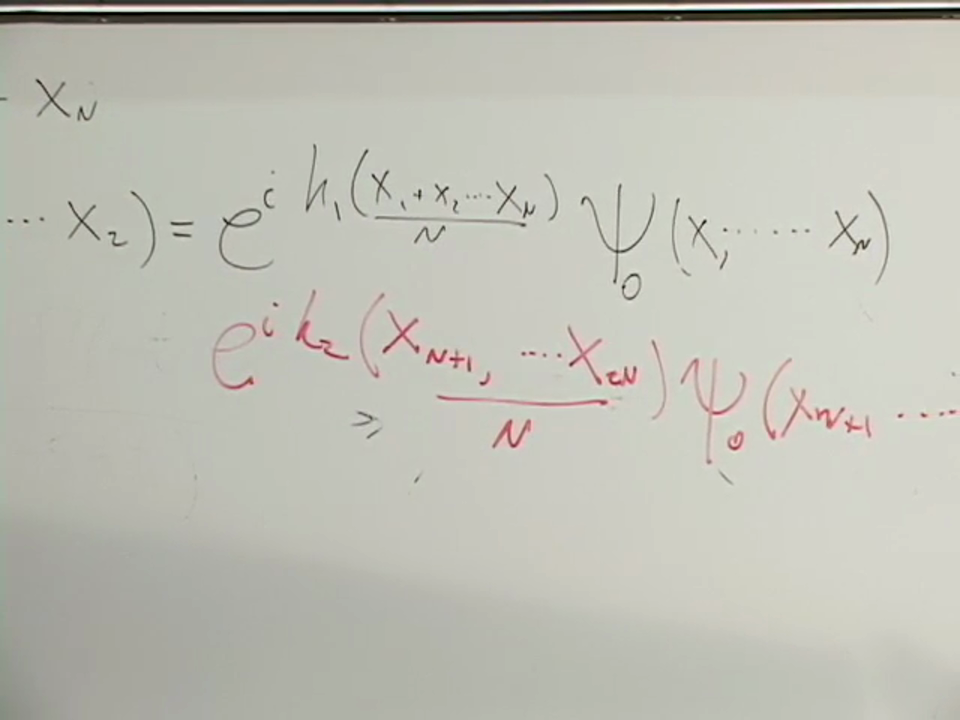
\includegraphics[width=0.76\textwidth]{lecture_06_figure_10.png}
  \caption{在施加端点重合条件之前的两链波函数。}
  \lectureframe{00:58:55}
  \label{fig:l06-endpoint-board}
\end{figure}

计算冗长但并不神秘。每个内部坐标都可以分解为振子模式，因此连接重叠、时间演化和最终投影都归结为高斯振子代数。尚未确定的是连接后弦的寿命\(\tau\)。

\begin{classroomqa}
\audiencequestion{黑色和红色波函数是相加还是相乘？\lecturetimestamp{01:02:26}}
\lecturerresponse{相乘。两个独立系统的张量积态在坐标基下由它们波函数的乘积表示。相加将描述各种备选可能性的叠加，而不是两条入射弦的同时存在。}
\end{classroomqa}

\begin{classroomqa}
\audiencequestion{为什么要对中间时间\(\tau\)积分？\lecturetimestamp{01:04:04}}
\lecturerresponse{连接后的弦并未被赋予固定的寿命。费曼规则是对所有允许的历史求和振幅。在这一描述中，剩余的连续历史参数就是连接与分裂之间的时间，因此求和变为对\(0\leq\tau<\infty\)的积分。}
\end{classroomqa}

\section{从传播时间到贝塔函数}

在计算完振子重叠之后，结果可以整理为
\begin{equation}
  \mathcal A(s,t)
  \propto
  \int_0^\infty d\tau\,
  e^{\tau(s+1)}
  \bigl(1-e^{-\tau}\bigr)^{-t-1}
  e^{-\tau}.
  \label{eq:l06-tau-integral}
\end{equation}
最后的\(e^{-\tau}\)保持可见，因为它是下一步所需的雅可比因子。等价地，第一个和最后一个指数因子合并为\(e^{s\tau}\)。

\begin{figure}[H]
  \centering
  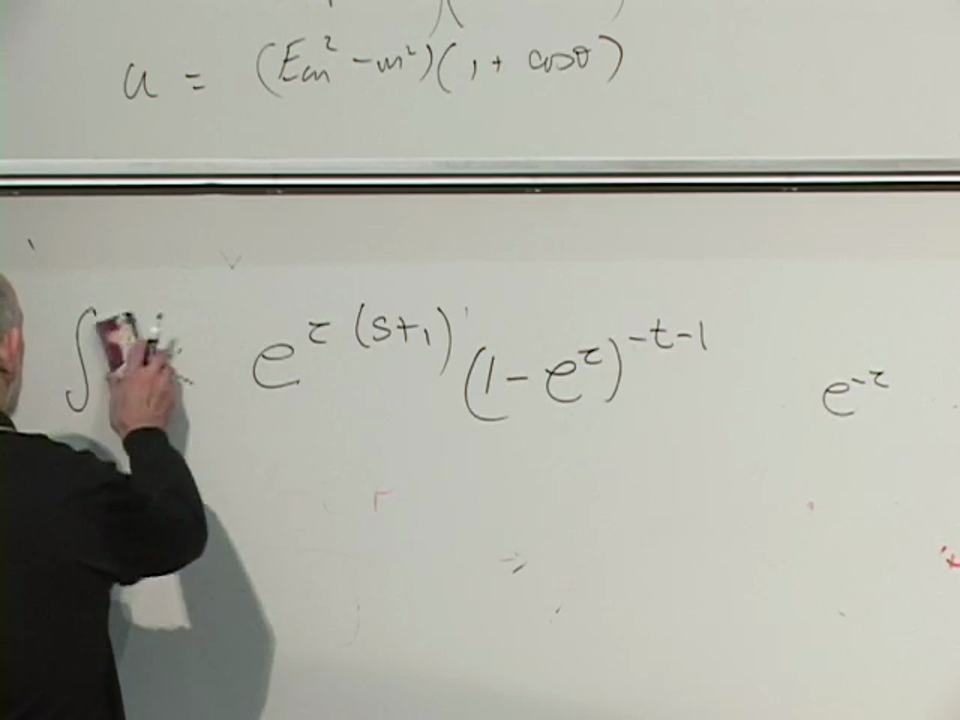
\includegraphics[width=0.76\textwidth]{lecture_06_figure_11.png}
  \caption{振子计算之后的传播时间被积函数；单独的\(e^{-\tau}\)因子提供变量替换的雅可比行列式。}
  \lectureframe{01:06:45}
  \label{fig:l06-tau-integral-board}
\end{figure}

现在令
\begin{equation}
  z=e^{-\tau},
  \qquad
  dz=-e^{-\tau}\,d\tau.
  \label{eq:l06-z-substitution}
\end{equation}
当\(\tau\)从\(0\)变到\(\infty\)时，\(z\)从\(1\)变到\(0\)。负号使积分限反转，得到
\begin{equation}
  \mathcal A(s,t)
  \propto
  \int_0^1
  z^{-s-1}(1-z)^{-t-1}\,dz.
  \label{eq:l06-beta-integral}
\end{equation}

\begin{figure}[H]
  \centering
  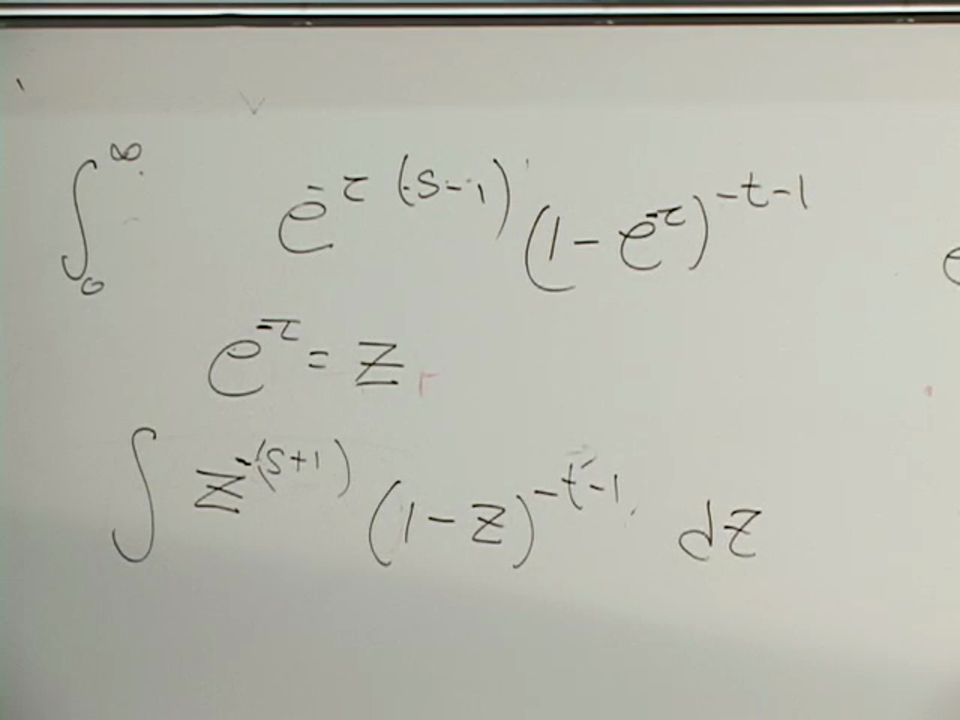
\includegraphics[width=0.74\textwidth]{lecture_06_figure_12.png}
  \caption{代换\(z=e^{-\tau}\)使欧拉贝塔积分显现出来。}
  \lectureframe{01:08:49}
  \label{fig:l06-beta-integral-board}
\end{figure}

该积分在其端点收敛之处直接有定义，在其他地方则由解析延拓定义。它就是欧拉贝塔函数：
\begin{equation}
  B(-s,-t)
  =
  \frac{\Gamma(-s)\Gamma(-t)}{\Gamma(-s-t)}.
  \label{eq:l06-beta-gamma}
\end{equation}

\begin{figure}[H]
  \centering
  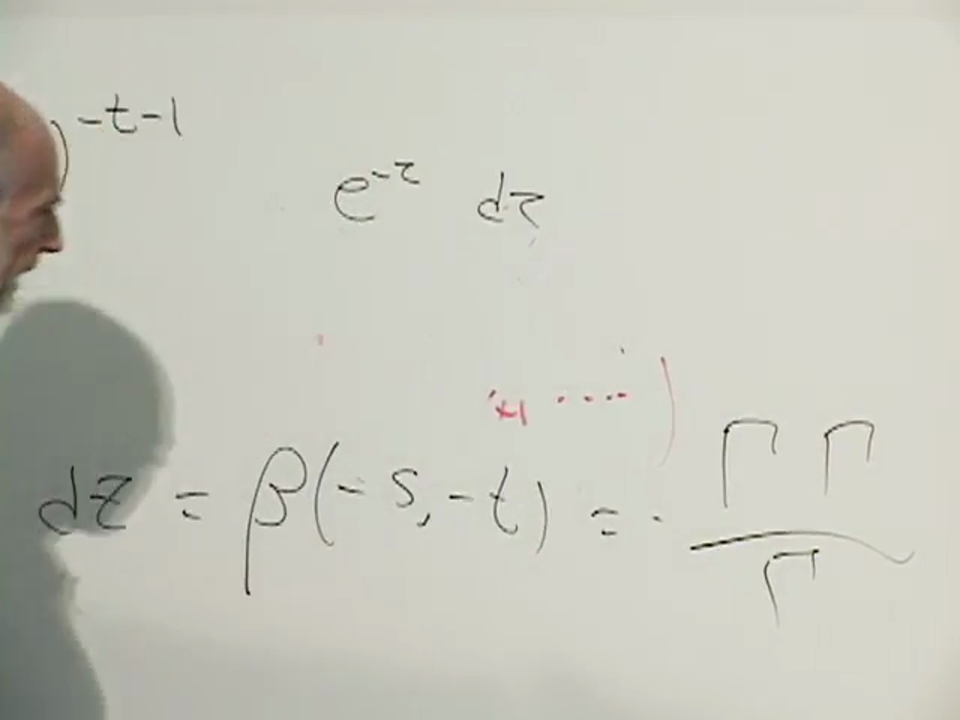
\includegraphics[width=0.72\textwidth]{lecture_06_figure_13.png}
  \caption{黑板上将变换后的积分等同于\(B(-s,-t)\)，并开始恢复其伽马函数形式。}
  \lectureframe{01:12:24}
  \label{fig:l06-beta-gamma-board}
\end{figure}

通道对称性现在是初等的。在\(z\mapsto1-z\)下，
\begin{equation}
  \int_0^1 z^{-s-1}(1-z)^{-t-1}\,dz
  =
  \int_0^1 z^{-t-1}(1-z)^{-s-1}\,dz.
\end{equation}
因此\(\mathcal A(s,t)=\mathcal A(t,s)\)。一个由两条弦连接、随后分裂所构造的过程，自动也包含了交叉描述。
\editorialnote{讲座在贝塔函数的自变量中省略了Regge斜率与截距。在标准记号中，人们把\(s,t\)替换为相应的线性轨迹\(\alpha(s),\alpha(t)\)。对偶性与变量替换论证不变。}

\begin{classroomqa}
\audiencequestion{伽马函数之比类似于组合学中的阶乘表达式。是否存在直接的物理计数解释？\lecturetimestamp{01:13:22}}
\lecturerresponse{在整数自变量处，贝塔函数与诸如\(n!\,m!/(n+m)!\)之比有关，但这里并未断言任何组合机制。同一个特殊函数恰好也来自世界面积分；这一相似性并不是发现该振幅所经由的途径。}
\end{classroomqa}

为什么一个世界面可以在两个通道中被读取，其仍然隐藏的原因是对称性。它允许把面像太妃糖一样拉伸而不改变振幅，从而把长的直接通道传播区域转变为交叉通道交换图像。这一几何解释推迟到下一讲。

\section{散射检验所确立的内容}
\enlargethispage{3\baselineskip}
\begingroup
\setlength{\medskipamount}{3pt plus 1pt minus 1pt}

离散的连接图像引出了最后一组问题。

\begin{classroomqa}
\audiencequestion{如果两条由\(n\)个组分构成的链在其端点处连接，结果是否为\(2n-1\)，并且这会改变费米子宇称吗？\lecturetimestamp{01:16:16}}
\lecturerresponse{在强子端点图像中，相接触的端点对可以被视为一对相互湮灭的粒子-反粒子，因此计数减少二，而不是一。在连续极限下，\(2n\)与\(2n-2\)之间的有限差异无关紧要，但保持费米子宇称并非无关紧要。点阵组分只是连续弦的一个调节器，而不是字面意义上的基本珠子。}
\end{classroomqa}

\begin{classroomqa}
\audiencequestion{后续讨论会继续深入到超弦的完整数学吗？\lecturetimestamp{01:18:05}}
\lecturerresponse{只会用到部分选定的推论。当前的路径是通过世界面对称性和紧致化，随后是1990年代中期发展出的另一个不同出发点：M理论。其目的是从一个视角达到相同的物理，在该视角下若干原本复杂的特征变得透明。}
\end{classroomqa}

\begin{classroomqa}
\audiencequestion{这一连接规则只是来自介子碰撞的一条线索吗？\lecturetimestamp{01:20:02}}
\lecturerresponse{介子散射提供了历史上的线索，但该规则对开弦是普遍的。同样的拓扑描述了开弦光子与其他开弦态的碰撞。两条闭弦通过类似的构造连接与分裂，中间区域有一条闭弦。}
\end{classroomqa}

\begin{classroomqa}
\audiencequestion{该计算是否只在弦态为费米子时适用？\lecturetimestamp{01:20:56}}
\lecturerresponse{不。最初的Veneziano计算属于玻色开弦。超弦需要额外的费米自由度并修改被积函数的细节，但连接、传播、投影以及世界面对偶的逻辑仍然密切类似。}
\end{classroomqa}

在振子谱中发现自旋为一或自旋为二的态是有启发性的，但并非决定性的。它们的散射振幅提供了更强的检验。光子振幅服从与电荷守恒和规范不变性相关的恒等式；引力子振幅服从无质量自旋二场的相应约束。弦态在与有质量和无质量态的相互作用中以及彼此之间的相互作用中通过了这些检验。这就是为什么光子和引力子标签成为物理上的认定，而不是仅基于极化计数的猜测。
\editorialnote{用现代语言来说，这些检验被编码在非物理极化的解耦、规范Ward恒等式以及无质量自旋二态的普适低能耦合中。}

\begin{classroomqa}
\audiencequestion{电荷本身在弦描述中来自何处？\lecturetimestamp{01:24:03}}
\lecturerresponse{这个问题在讲座结束时仍然悬而未决。其答案需要弦理论的内部结构与端点结构，而这些尚未被引入，因此它属于随后的讨论，而不属于这一散射推导。}
\end{classroomqa}
\endgroup

\chapter{世界面、威克转动与道对偶}

\lectureoverview{粒子描出一条世界线；弦则扫出一个世界面。对二者中任何一个进行量子化都需要对历史求和，但洛伦兹号差的求和是振荡的，难以定义。把世界面时间变为虚坐标后，得到一个由拉普拉斯方程支配的欧几里得理论。其共形对称性随即把四弦相互作用的裂缝状曲面变成带有四个边界插入点的圆盘，于是直接道与交叉道之间的对称性变得可见。}

\section{从世界线到对历史求和}

先从一个自由粒子开始。在非相对论力学中，它的位置是函数\(\mathbf x(t)\)，并且，在把质量取为1后，其作用量为
\begin{equation}
  S_{\mathrm{NR}}[\mathbf x]
  =\frac12\int_{t_1}^{t_2}\dot{\mathbf x}^{\,2}\,dt.
  \label{eq:l07-nr-action}
\end{equation}
对于相对论性描述，更自然的做法是把时间和空间放进一个矢量\(X^\mu(\tau)\)中，并沿轨迹用\(\tau\)参数化。相应的二次表达式为
\begin{equation}
  S_{\mathrm{rel}}[X]
  =\frac12\int_{\tau_1}^{\tau_2}
  \frac{dX^\mu}{d\tau}\frac{dX_\mu}{d\tau}\,d\tau.
  \label{eq:l07-rel-action}
\end{equation}
上指标与下指标编码了时间与空间之间的洛伦兹号差。
\editorialnote{这里使用的是在固定世界线参数化下的二次相对论作用量。显式重参数化不变的替代方案正比于固有长度，这一点在讲座后文会提到。}

\begin{figure}[H]
  \centering
  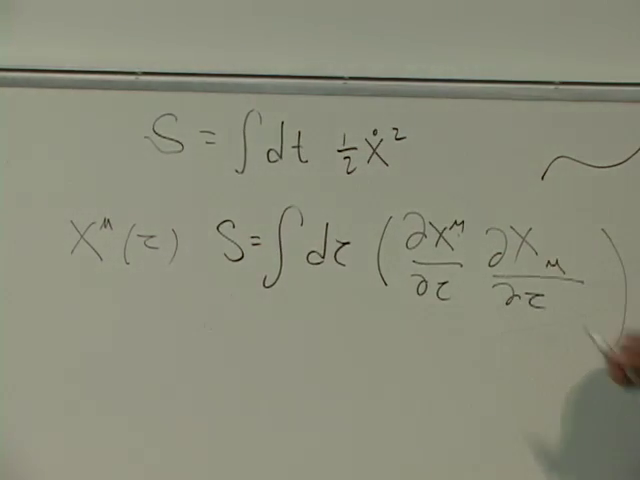
\includegraphics[width=0.72\textwidth]{lecture_07_figure_01.png}
  \caption{非相对论作用量及其相对论二次对应物一起写在黑板上。}
  \lectureframe{00:03:35}
  \label{fig:l07-particle-actions}
\end{figure}

在经典层面，人们固定端点并改变路径。自由粒子随后沿一条速度恒定的直线世界线运动。量子力学问的是另一个问题。它并不在端点之间选出一条轨迹；它问的是从一点出发并在另一点被探测到的振幅。每一条介于其间的路径都贡献一个相位，
\begin{equation}
  K(2,1)=\int_{X(1)}^{X(2)}\!\mathcal D X\,
  e^{iS[X]}.
  \label{eq:l07-feynman-integral}
\end{equation}
泛函积分是在无限维路径空间上的积分，而不是已经出现在作用量内部的普通积分。

\begin{figure}[H]
  \centering
  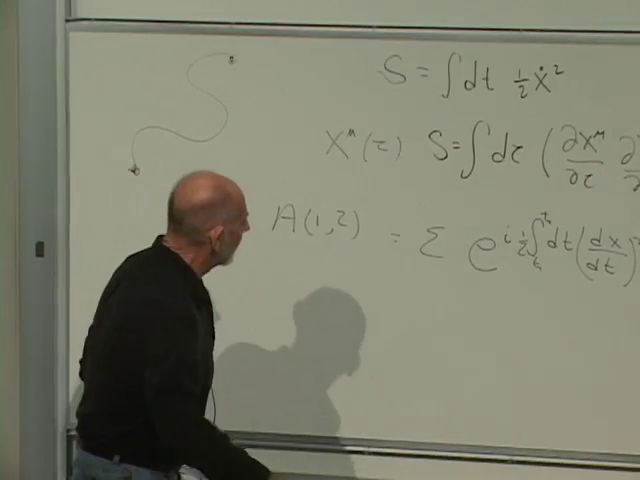
\includegraphics[width=0.72\textwidth]{lecture_07_figure_02.png}
  \caption{在取遍所有轨迹的求和之前，一条代表性路径以及赋予它的相位。}
  \lectureframe{00:06:21}
  \label{fig:l07-path-integral-board}
\end{figure}

用相对论语言来说，这个从点到点的振幅是一个传播子。对于相互作用，若干世界线段相遇。它们的作用量相加，相遇点被积分掉，并对外部粒子符合要求的图求和。因此，熟悉的费曼图展开已经隐含在对历史求和的指令之中。

符号\(S\)在这里将表示一个作用量。它既与熵无关，也与讲座接近末尾处使用的曼德尔施塔姆变量\(s\)无关。这种记号上的共用是传统使然，而非富有启发性。

\section{把时间转向侧面}

\eqref{eq:l07-feynman-integral}立刻存在一个问题。每个因子\(e^{iS}\)的模都是1。因此，一条剧烈振荡的轨迹和经典直线以相同的绝对权重进入；只有它们的相位不同。相消干涉恢复了经典行为，但这并不使形式积分成为一个普通的收敛对象。

通过
\begin{equation}
  \tau=\alpha s,
  \qquad
  d\tau=\alpha\,ds,
  \qquad
  \frac{dX}{d\tau}=\frac{1}{\alpha}\frac{dX}{ds}.
\end{equation}
引入一个新参数\(s\)。于是二次作用量按如下方式重新标度：
\begin{equation}
  \frac12\int d\tau
  \left(\frac{dX}{d\tau}\right)^2
  =
  \frac{1}{2\alpha}\int ds
  \left(\frac{dX}{ds}\right)^2.
  \label{eq:l07-rescaled-action}
\end{equation}
选择对应于\(\alpha=-i\)的围道会把振荡权重变为
\begin{equation}
  e^{iS}
  \longrightarrow
  \exp\!\left[-\frac12\int ds
  \left(\frac{dX}{ds}\right)^2\right]
  =e^{-S_E}.
  \label{eq:l07-euclidean-particle}
\end{equation}

\begin{figure}[H]
  \centering
  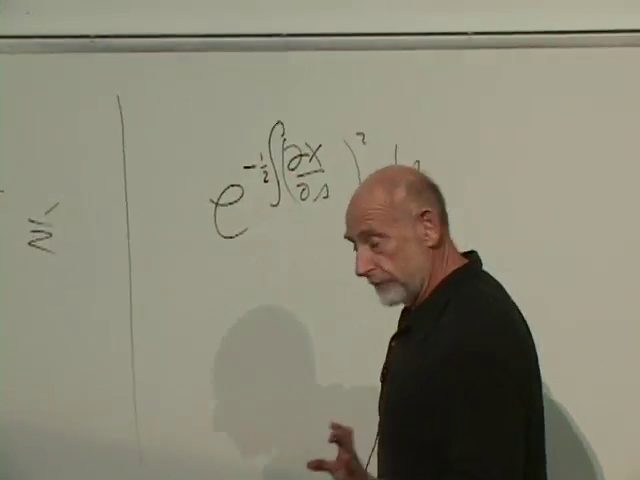
\includegraphics[width=0.66\textwidth]{lecture_07_figure_03.png}
  \caption{虚时间替换后的欧几里得粒子权重；指数为实且非正。}
  \lectureframe{00:16:20}
  \label{fig:l07-particle-wick}
\end{figure}

一条跑到很远再返回的路径，或者一条不跑远却快速扭动的路径，都有很大的正\(S_E\)，因而被指数压低。结果是一个维纳型积分，对此存在严格的收敛理论。从实\(\tau\)继承来的端点位于一条虚\(s\)围道上。实践中，人们在收敛区域内计算欧几里得对象，并把答案解析延拓回物理的洛伦兹变量。这一操作就是威克转动：时间是为了计算而被转向侧面，而不是被丢弃。

\section{从世界线到世界面}

点粒子有一条世界线。开弦扫出一条带子，闭弦扫出一根管子。坐标\((\sigma,\tau)\)标记这个二维世界面上的点，而
\begin{equation}
  X^\mu=X^\mu(\sigma,\tau)
  \label{eq:l07-embedding}
\end{equation}
给出被标记点的时空位置。知道所有函数\(X^\mu\)就完全确定了弦的整个历史。

二次洛伦兹世界面作用量具有与普通振动弦相同的动能减势能结构：
\begin{equation}
  S_{\mathrm{ws}}[X]
  =\frac{T_s}{2}\int d\tau\,d\sigma\,
  \left[
    \partial_\tau X^\mu\partial_\tau X_\mu
    -
    \partial_\sigma X^\mu\partial_\sigma X_\mu
  \right].
  \label{eq:l07-lorentzian-worldsheet}
\end{equation}
整体张力\(T_s\)固定了标度；本讲在专注于导数结构时将其略去。

\begin{figure}[H]
  \centering
  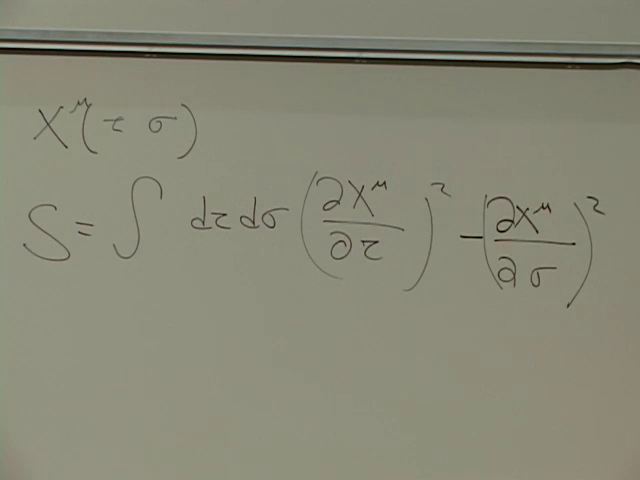
\includegraphics[width=0.72\textwidth]{lecture_07_figure_04.png}
  \caption{\(X^\mu(\sigma,\tau)\)的洛伦兹世界面作用量，及其动能减势能的符号。}
  \lectureframe{00:24:26}
  \label{fig:l07-worldsheet-action}
\end{figure}

弦振幅通过将此作用量指数化并对连接指定初末弦构型的所有曲面求和得到：
\begin{equation}
  \mathcal A=\int\mathcal D X\,e^{iS_{\mathrm{ws}}[X]}.
  \label{eq:l07-surface-integral}
\end{equation}
同一规则处理两弦变为两弦、两弦变为三弦，或任何其他允许的外腿构型。不同的世界面拓扑也属于该求和。添加洞是点粒子图展开中添加圈阶的弦对应物。

\begin{figure}[H]
  \centering
  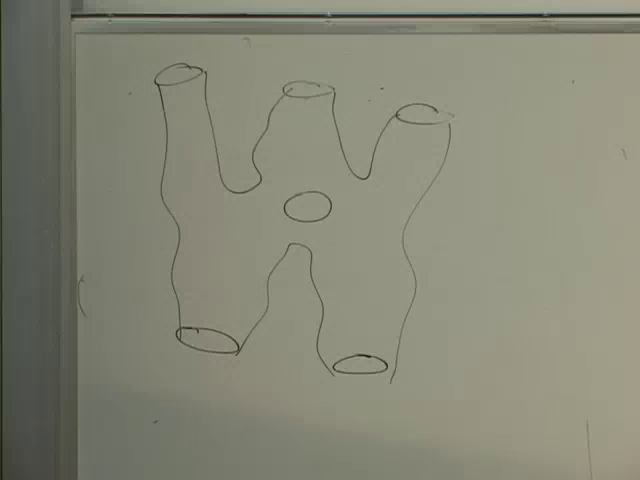
\includegraphics[width=0.66\textwidth]{lecture_07_figure_05.png}
  \caption{连接若干外弦的曲面，其中一个洞代表不同的世界面拓扑。}
  \lectureframe{00:27:14}
  \label{fig:l07-surface-topology}
\end{figure}

\begin{classroomqa}
\audiencequestion{对于点电子，\(\sigma\)导数是否直接消失？\lecturetimestamp{00:27:56}}
\lecturerresponse{点粒子首先就没有\(\sigma\)坐标。然而两幅图像是相联系的：当外态相对于弦标度很轻且过程能量很低时，弦振幅重现普通的点粒子费曼图。该极限不仅仅是把一个导数设为零。}
\end{classroomqa}

曲面积分与路径积分有相同的收敛问题。在对世界面时间做威克转动后，其稳定的欧几里得形式为
\begin{equation}
  \begin{aligned}
    S_{E,\mathrm{ws}}[X]
    &=\frac{T_s}{2}\int d\tau\,d\sigma\,
      \left[
        \partial_\tau X^\mu\partial_\tau X_\mu
        +\partial_\sigma X^\mu\partial_\sigma X_\mu
      \right],\\
    \mathcal A_E&=\int\mathcal D X\,e^{-S_{E,\mathrm{ws}}}.
  \end{aligned}
  \label{eq:l07-euclidean-worldsheet}
\end{equation}
两个导数现在都以相同的正号进入。剧烈振动或大幅拉伸的曲面具有大的欧几里得作用量并被压低。

\begin{figure}[H]
  \centering
  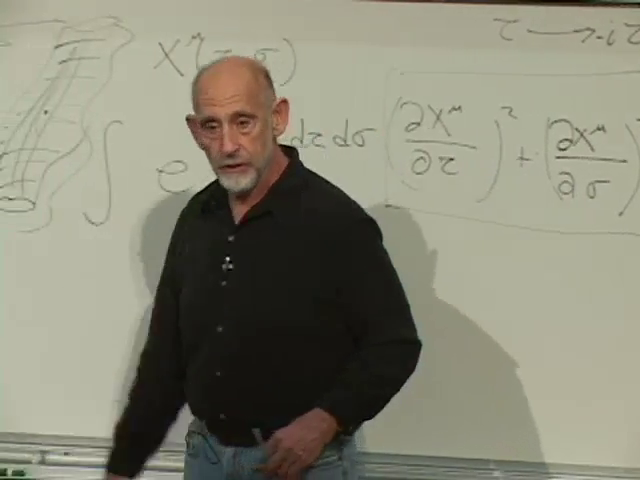
\includegraphics[width=0.72\textwidth]{lecture_07_figure_06.png}
  \caption{在\(\tau\)被转动到虚时间后的正欧几里得世界面密度。}
  \lectureframe{00:34:29}
  \label{fig:l07-worldsheet-wick}
\end{figure}

还有一种几何上直接的表述。可以给相对论性粒子赋予一个正比于其路径固有长度的作用量；可以给弦赋予一个正比于其世界面时空面积的作用量。后者即南部--后藤作用量。这里所用的二次世界面形式习惯上称为波利亚科夫形式，对当前计算要容易得多。
\editorialnote{本讲包含一段关于历史命名的幽默讨论，也提到了相关的刘维尔作用量和狄利克雷边界条件。该推导无需优先权主张：只用到面积表述与辅助度规表述的等价性。}

\section{欧几里得运动方程}

坐标\(\sigma\)和\(\tau\)只是世界面上的标签。因此下一个问题不可避免：哪些重标记使理论保持不变？答案最容易从运动方程看出。对\eqref{eq:l07-euclidean-worldsheet}变分，逐分量给出
\begin{equation}
  \partial_\tau^2X^\mu+\partial_\sigma^2X^\mu=0.
  \label{eq:l07-laplace}
\end{equation}
在威克转动之前，相对符号为负，这是一个波动方程。在欧几里得号差下两个符号都为正，因此它是二维拉普拉斯方程。

\begin{classroomqa}
\audiencequestion{这是振动鼓面的方程吗？
\lecturetimestamp{00:41:50}}
\lecturerresponse{它与之密切相关，但振动鼓面还带有一个真实时间坐标，因此服从波动方程。这里的方程是欧几里得拉普拉斯方程。无电荷区域中的静电势提供了一个更直接的熟悉例子。}
\end{classroomqa}

\begin{classroomqa}
\audiencequestion{作用量含有一阶导数。为什么其方程含有二阶导数？\lecturetimestamp{00:42:44}}
\lecturerresponse{对一阶导数的二次项变分并分部积分，会把一个导数移到该一阶导数上。这是场论版本的\(\dot x^{\,2}\)出现在作用量中而产生运动方程中的\(\ddot x\)。}
\end{classroomqa}

\begin{figure}[H]
  \centering
  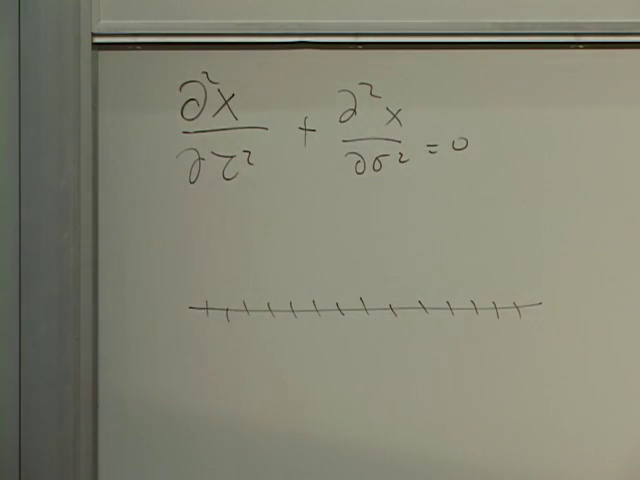
\includegraphics[width=0.68\textwidth]{lecture_07_figure_07.png}
  \caption{带正号的拉普拉斯方程，以及用于解释其二阶导数的第一行离散表达式。}
  \lectureframe{00:43:30}
  \label{fig:l07-laplace-board}
\end{figure}

为看清几何，先用间距\(\epsilon\)离散化一个坐标。一阶导数是相邻差分，而二阶导数是相邻差分之差：
\begin{equation}
  \frac{d^2X}{ds^2}\bigg|_{2}
  \longrightarrow
  \frac{X(3)-2X(2)+X(1)}{\epsilon^2}.
  \label{eq:l07-second-difference}
\end{equation}

\begin{figure}[H]
  \centering
  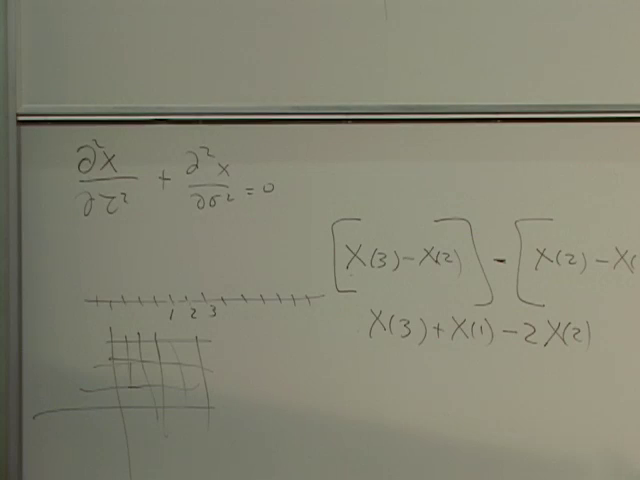
\includegraphics[width=0.72\textwidth]{lecture_07_figure_08.png}
  \caption{编号行、小点阵块，以及二阶导数的有限差分展开。}
  \lectureframe{00:45:51}
  \label{fig:l07-finite-difference-board}
\end{figure}

现在离散化\((\sigma,\tau)\)平面。将中心点\(5\)的四个最近邻标记为\(1,2,3,4\)。方程\eqref{eq:l07-laplace}变为
\begin{equation}
  X(1)+X(2)+X(3)+X(4)-4X(5)=0,
\end{equation}
或
\begin{equation}
  X(5)=\frac14\bigl[X(1)+X(2)+X(3)+X(4)\bigr].
  \label{eq:l07-mean-value}
\end{equation}

\begin{figure}[H]
  \centering
  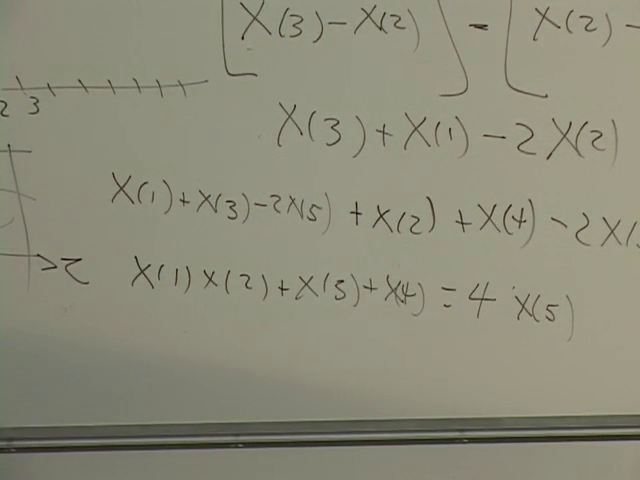
\includegraphics[width=0.72\textwidth]{lecture_07_figure_09.png}
  \caption{完成后的二维有限差分方程：中心值等于其四个相邻点的平均值。}
  \lectureframe{00:48:26}
  \label{fig:l07-mean-value-board}
\end{figure}

这一均值性质对任意取向的无穷小正方形都成立。它是拉普拉斯方程的局部几何内容，也是通向共形对称性的桥梁。

\section{共形坐标}

考虑从\((\sigma,\tau)\)到\((\sigma',\tau')\)的变换。一般的形变会把一个小正方形变为任意四边形。这里相关的特殊变换则把每个无穷小正方形变为另一个无穷小正方形，可能带有旋转和缩放。等价地说，它们保持曲线相交处的角度。这些就是共形变换。

\begin{figure}[H]
  \centering
  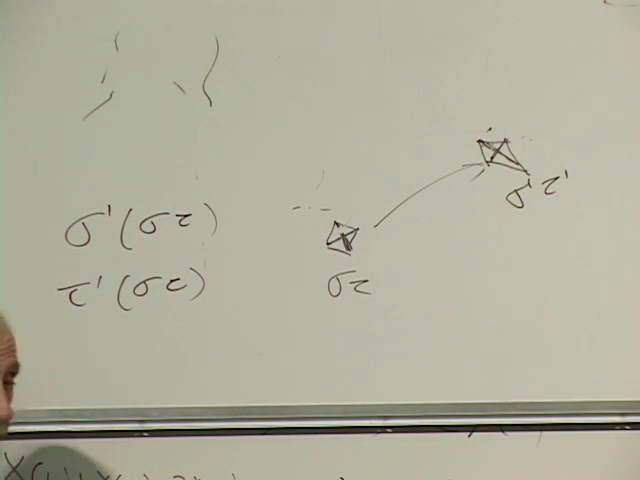
\includegraphics[width=0.68\textwidth]{lecture_07_figure_10.png}
  \caption{一个局部正方形被映射为另一个小图形，同时检验其角度是否被共形地保持。}
  \lectureframe{00:53:25}
  \label{fig:l07-conformal-board}
\end{figure}

\begin{classroomqa}
\audiencequestion{如果角度被保持，那么该变换基本上只是旋转吗？\lecturetimestamp{00:53:31}}
\lecturerresponse{只在局部如此，而且即便在局部，也允许一个共同的尺度变化。局部的旋转和尺度因子可以逐点变化，因此坐标网格可以弯曲，在一个区域膨胀，在另一个区域收缩，同时保持无穷小形状。}
\end{classroomqa}

保角映射不必保持大小。如果大小也在各处固定，那么可能性就会坍缩为小得多的刚性类，即平移和旋转。共形映射则保持局部形状。这就是为什么地图投影可以保持一个小岛的形状，却极大地扭曲其面积。

\begin{classroomqa}
\audiencequestion{共形映射等价于说坐标系是平坦的吗？\lecturetimestamp{00:55:35}}
\lecturerresponse{不。平坦性和共形性是两种不同的陈述。共形映射可以使用弯曲的坐标线；它所保持的是相交曲线之间的角度。墨卡托型地图投影就是一个熟悉的例子，它在保持局部形状的同时具有显著的尺度畸变。}
\end{classroomqa}

在二维情形中，所需的变换局部地由复坐标的解析函数生成
\begin{equation}
  z=\sigma+i\tau.
\end{equation}
有限边界可以显著改变外观。一个正方形区域可以被映射为一个光滑区域，原来的角被送到新边界上的普通点，而不是其视觉上突出的点。这并不矛盾：共形性是局部的内部条件，而映射在其正则之处保持无穷小角度。

\begin{classroomqa}
\audiencequestion{这种坐标自由度是否就是先前那个
join--split图可以被选为对称形式的原因？
\lecturetimestamp{00:56:32}}
\lecturerresponse{是的。正是这种保持世界面方程的共形自由度，让我们能够把别扭的相互作用带替换为更对称的区域。剩余的自由度并不会移除物理的
join--split参数；它只是把该参数重新包装为边界插入点的相对位置。}
\end{classroomqa}

\section{带缝薄片与圆盘}

回到四弦散射。两条开弦进入，它们的端点相接，合并后的弦传播，随后又分裂。画成平坦世界面时，这一过程是一条从两端被切开的无限长条带。两条缝的尖端之间的间隔\(\tau_0\)是中间弦的寿命，而振幅对它积分。

\begin{figure}[H]
  \centering
  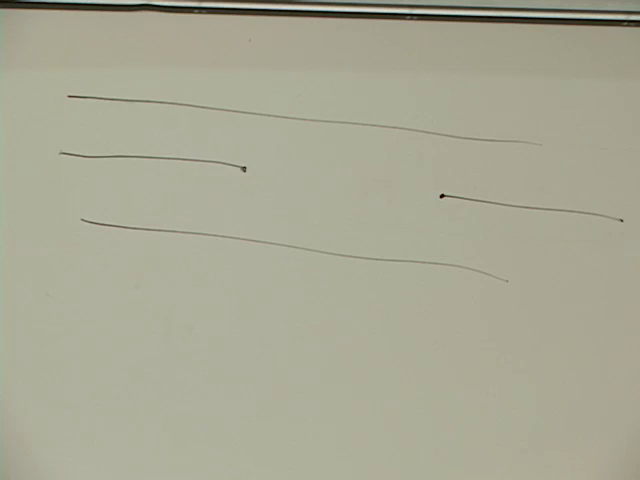
\includegraphics[width=0.72\textwidth]{lecture_07_figure_11.png}
  \caption{表示两条开弦相接、共同传播并再次分裂的双缝长条带。}
  \lectureframe{01:00:20}
  \label{fig:l07-slit-strip}
\end{figure}

欧几里得化之后，这一区域上的嵌入场满足拉普拉斯方程。因此共形不变性允许把带缝长条带映射为圆盘。看清其拓扑的一种方式是用同心圆叶状分层圆盘，并连续形变这些闭合曲线，直到它们填满带缝区域。无穷远处的端点在映射下成为特殊的边界点。

\begin{figure}[H]
  \centering
  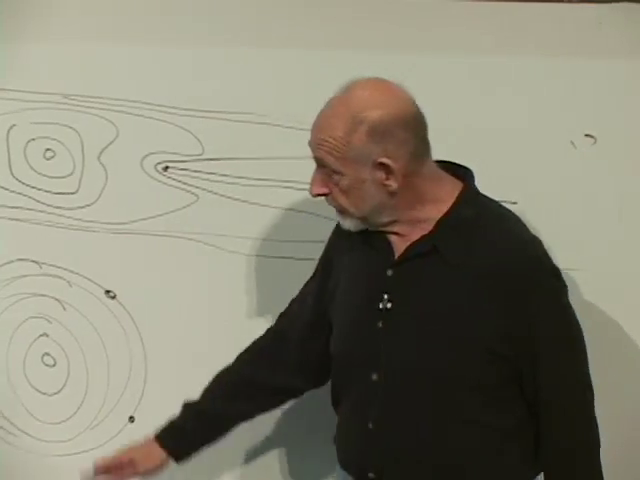
\includegraphics[width=0.72\textwidth]{lecture_07_figure_12.png}
  \medskip

  \begin{adjustbox}{max width=\linewidth}
  \begin{tikzpicture}[x=0.75cm,y=0.75cm]
    \draw[thick] (-5,1.2) -- (-1.2,1.2) -- (-0.35,0.35);
    \draw[thick] (-5,-1.2) -- (-1.2,-1.2) -- (-0.35,-0.35);
    \draw[thick] (0.35,0.35) -- (1.2,1.2) -- (5,1.2);
    \draw[thick] (0.35,-0.35) -- (1.2,-1.2) -- (5,-1.2);
    \draw[->,thick] (5.6,0) -- (7.0,0);
    \draw[thick] (9.0,0) circle (1.45);
    \foreach \a in {40,140,220,320} \fill (9.0,0) ++(\a:1.45) circle (1.5pt);
    \node[below] at (0,-1.65) {slit strip};
    \node[below] at (9.0,-1.65) {disc};
  \end{tikzpicture}
  \end{adjustbox}
  \caption{黑板上的等值线比较，以及从带缝长条带到圆盘的共形映射的清晰示意图。四个外部端点成为四个特殊的边界点。}
  \lectureframe{01:04:46}
  \label{fig:l07-strip-to-disc}
\end{figure}

外部态在这种坐标变换中并未丢失。动量、粒子类型和振子能级必须插入到四个特殊点上。承载这些信息的形式对象是顶点算子。它们的详细构造留待以后，但其作用已经清楚：它们把原本均匀的世界面路径积分变为一个指定的散射实验。

在利用圆盘的共形变换将三个边界点移到方便的参考位置之后，还剩下一个实相对位置。它可以由四个有序边界点的交比来表示。这就是旧的寿命\(\tau_0\)的圆盘版本。

\begin{figure}[H]
  \centering
  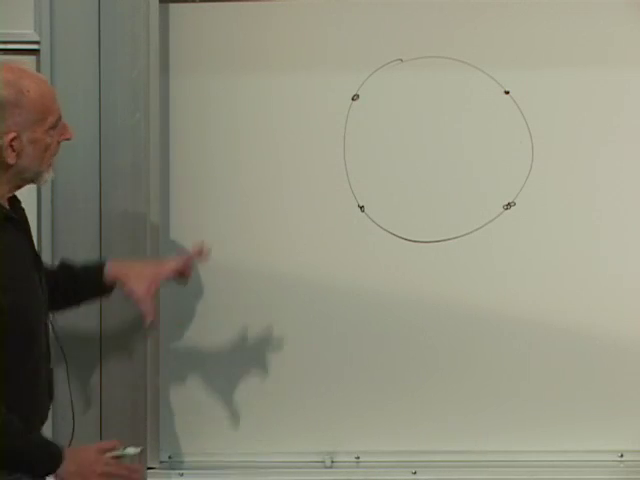
\includegraphics[width=0.62\textwidth]{lecture_07_figure_13.png}
  \caption{圆盘边界上的四个插入点。共形自由度除去了它们有序位形中除一个实模数之外的全部模数。}
  \lectureframe{01:10:55}
  \label{fig:l07-four-points}
\end{figure}

因此寿命积分并没有消失。它变成了对那个剩余模数的积分。采用惯用坐标\(0<z<1\)，四点开弦积分取与上一讲中所得相同的形式，
\begin{equation}
  \mathcal A(s,t)\propto
  \int_0^1 z^{-s-1}(1-z)^{-t-1}\,dz.
  \label{eq:l07-modulus-integral}
\end{equation}

\section{同一个曲面的两个极限}

在模空间的一端，与入射对相关联的两个插入点彼此靠近。在缝条坐标中，这是连接与分裂之间的一段长间隔：一个直接道中间弦传播了很长时间。在另一端，另一对相邻的点彼此靠近。同一个曲面于是自然地被读作交叉道交换。这些描述在条带上看起来互不相关，但它们是一个圆盘积分的相邻边界极限。

回到上一讲的mostly-plus约定，
\begin{equation}
  -s=(k_1+k_2)^2,
  \qquad
  -t=(k_1+k_3)^2.
  \label{eq:l07-mandelstam}
\end{equation}
直接极限将极点组织在\(s\)中；交叉极限将极点组织在\(t\)中。
\editorialnote{在讲座接近尾声时，黑板上对Mandelstam不变量使用了简写符号，同时将\(s\)等同于正的中心-of-mass能量平方。方程\eqref{eq:l07-mandelstam}保持了第6讲中确立的mostly-plus约定。}

\begin{figure}[H]
  \centering
  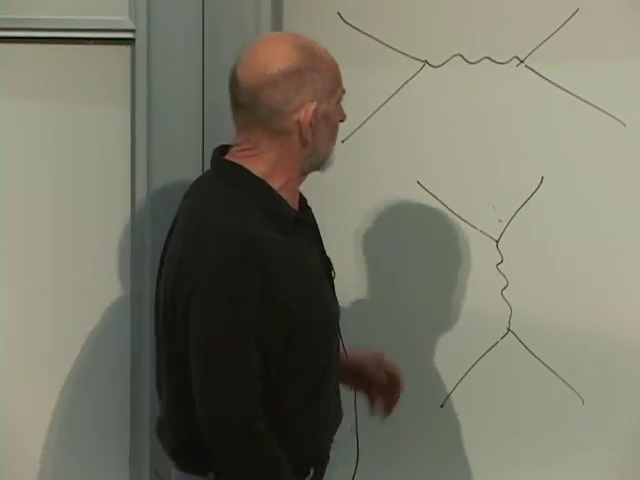
\includegraphics[width=0.62\textwidth]{lecture_07_figure_14.png}
  \caption{两个道图：在一个取向上是长传播，在交叉取向上是交换。}
  \lectureframe{01:19:27}
  \label{fig:l07-channel-diagrams}
\end{figure}

\begin{figure}[H]
  \centering
  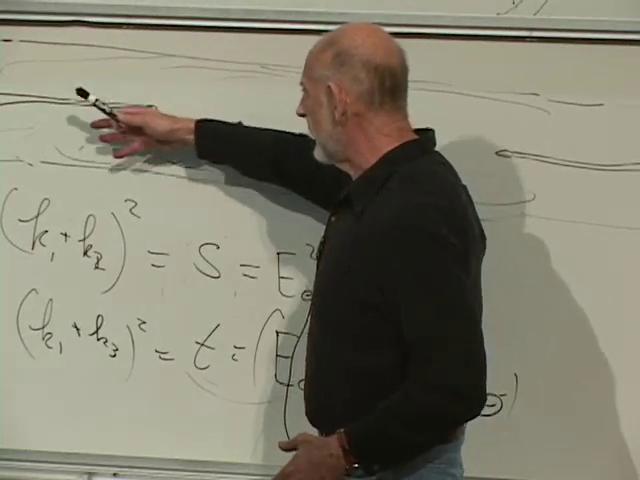
\includegraphics[width=0.72\textwidth]{lecture_07_figure_15.png}
  \caption{黑板回到\(s\)道和\(t\)道的动量配对，同时比较圆盘模数的两个极限。}
  \lectureframe{01:19:40}
  \label{fig:l07-st-board}
\end{figure}

因此一个解析对象同时提供了两种展开：
\begin{equation}
  \mathcal A(s,t)=\mathcal A(t,s).
\end{equation}
这就是道对偶。在最初的共振语言中，对直接道态求和竟也能编码交叉道交换，这显得不可思议。在欧几里得世界面上，共形对称性解释了为什么这两种描述属于同一个曲面。历史上，这一解释在Veneziano振幅于1969年被发现之后很快就出现了。

\begin{classroomqa}
\audiencequestion{是否也存在对应于交叉取向的缝条图像？\lecturetimestamp{01:20:49}}
\lecturerresponse{是的，但被称为时间的方向必须另行选取。同一个欧几里得曲面可以被切片，使得另一对外部端点位于遥远的过去和未来。正是这种替代切片方式，使得单个世界面允许多于一种道的解释。}
\end{classroomqa}

\begin{classroomqa}
\audiencequestion{弦保持连接的时间是否由耦合常数决定？\lecturetimestamp{01:21:39}}
\lecturerresponse{不会选出任何固定的寿命。寿命是一个积分变量，每一个值都有贡献。耦合控制连接与分裂的权重---等价地，即衰变强度---，并以相乘的方式进入振幅；它并不取代模数积分。}
\end{classroomqa}

\chapter{共形映射与开弦散射规定}

\lectureoverview{共形映射最初是作为二维静电学的一种实用对称性而出现的。复可微性把这种对称性变成了一种可计算的对称性：柯西--黎曼方程蕴含拉普拉斯方程，而与方向无关的复导数保持角度不变。有了这套工具，弦的世界面就可以画成条带、半平面、圆柱或圆盘，而物理不变。开弦散射于是变成圆盘上的高斯路径积分，动量插入位于其边界上，随后再对它们的不等价位置进行积分。}

\section{二维世界中的静电学}

我们从一个字面意义上的二维静电学问题开始。电荷及其场线被限制在一个平面内；它们并不只是运动恰好发生在平面内的普通三维电荷。于是高斯定律给出
\begin{equation}
  F(r)\propto \frac{1}{r},
  \qquad
  V(r)\propto \log r,
  \label{eq:l08-two-dimensional-coulomb}
\end{equation}
因为通量穿过的是一个周长按\(r\)增长的圆。

用标量势\(\phi\)来表示场。按照黑板上使用的符号约定，
\begin{equation}
  \mathbf E=\nabla\phi,
  \qquad
  \nabla\cdot\mathbf E=\rho,
\end{equation}
因此
\begin{equation}
  \nabla^2\phi
  =\frac{\partial^2\phi}{\partial x^2}
  +\frac{\partial^2\phi}{\partial y^2}
  =\rho.
  \label{eq:l08-poisson}
\end{equation}
在无电荷区域，这化为拉普拉斯方程，
\begin{equation}
  \nabla^2\phi=0.
  \label{eq:l08-laplace-phi}
\end{equation}
\editorialnote{许多电动力学教材定义
\(\mathbf E=-\nabla\Phi\)，在这种情况下，吸收常数后得到
\(\nabla^2\Phi=-\rho\)。本讲使用相反的势符号。无源方程以及所有共形论证都不变。}

\begin{figure}[H]
  \centering
  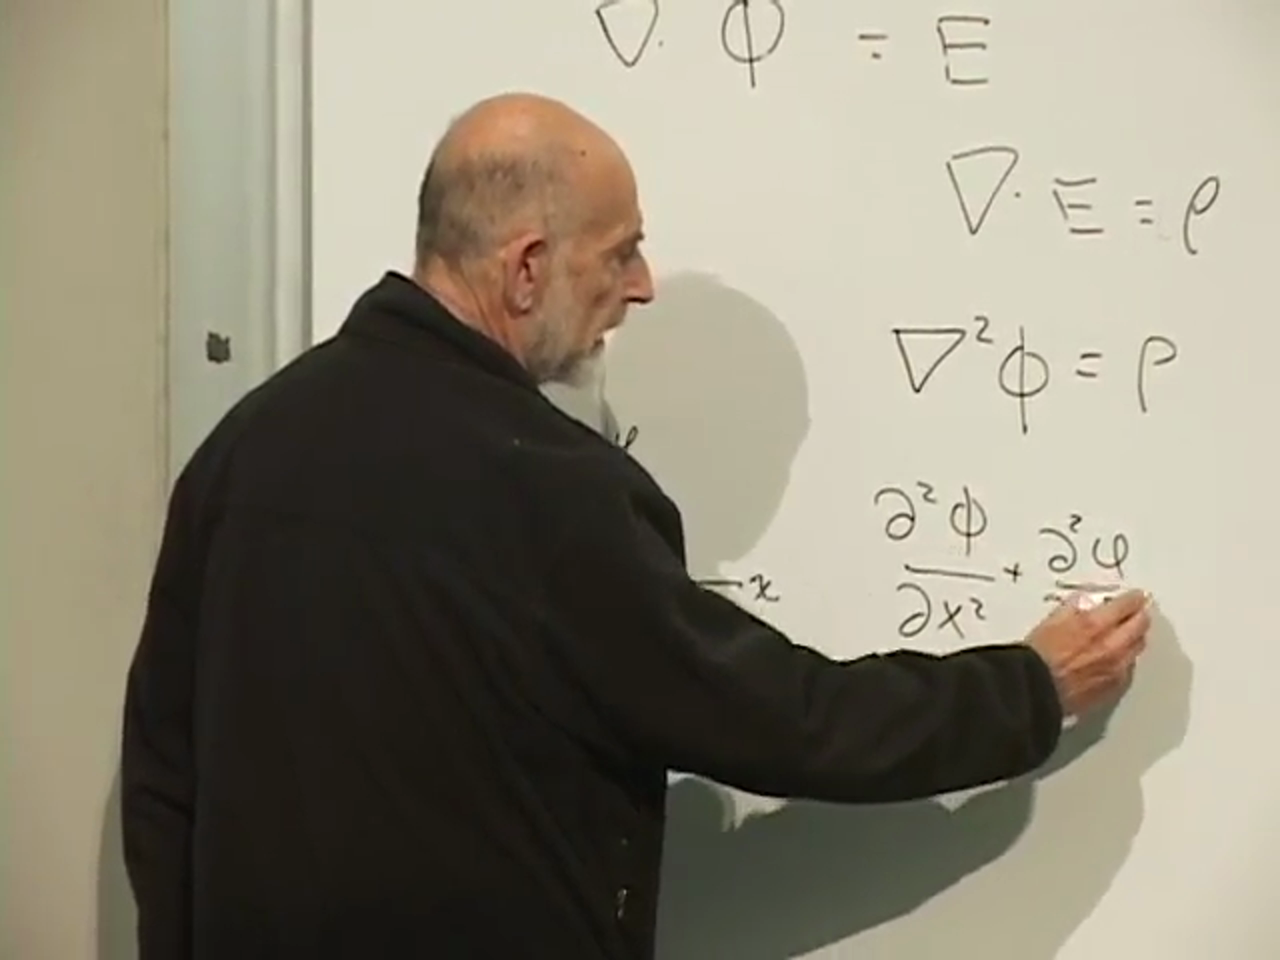
\includegraphics[width=0.72\textwidth]{lecture_08_figure_01.png}
  \caption{静电学方程展开为二维泊松算子。}
  \lectureframe{00:03:48}
  \label{fig:l08-electrostatics-board}
\end{figure}

两个空间导数之间的正号很重要。它使这个方程成为椭圆型方程，而不是波动方程。共形变换保持其无源形式，因此一个区域上的解可以连同其边界条件一起被搬到形状不同的区域上。这在静电学、二维流体流动和制图学中很有用，然后才在弦理论中有用。

\begin{classroomqa}
\audiencequestion{如果拉普拉斯算子为零，这是驻波方程吗？\lecturetimestamp{00:05:35}}
\lecturerresponse{不是。两个空间导数符号相同，而且没有时间导数。波动方程需要时间依赖，并具有洛伦兹式的相对符号。静电学之所以是静态的，正是因为没有任何东西在演化，包括波。}
\end{classroomqa}

\begin{classroomqa}
\audiencequestion{二维中有旋度吗？
\lecturetimestamp{00:06:06}}
\lecturerresponse{有，但它只有一个独立分量。对于
\(\mathbf E=(E_x,E_y)\)，
\[
  \operatorname{curl}_{2d}\mathbf E
  =\partial_yE_x-\partial_xE_y.
\]
可以把它想象为垂直于黑板的分量，尽管一个内禀二维的世界并不需要外部的垂直方向。在更高维中，相应的对象自然是一个反对称二形式。}
\end{classroomqa}

\section{没有优先方向的导数}

在原平面和像平面上引入复坐标：
\begin{equation}
  z=x+iy,
  \qquad
  w=u+iv,
  \qquad
  w=w(z).
  \label{eq:l08-complex-coordinates}
\end{equation}
这里\(x,y,u,v\)是实数。局部地，导数应当是
\begin{equation}
  \frac{dw}{dz}
  =\lim_{\Delta z\to0}\frac{\Delta w}{\Delta z}.
  \label{eq:l08-complex-derivative}
\end{equation}
与实直线不同，复平面允许无穷多个逼近方向。一个连续且通常光滑的映射不必沿每个方向给出相同的比值。

比较两种简单的逼近方式。沿\(x\)方向，\(dy=0\)，所以
\begin{equation}
  \left.\frac{dw}{dz}\right|_x
  =\frac{\partial u}{\partial x}
  +i\frac{\partial v}{\partial x}.
\end{equation}
沿\(y\)方向，\(dx=0\)，并且
\begin{equation}
  \left.\frac{dw}{dz}\right|_y
  =\frac{1}{i}\frac{\partial u}{\partial y}
  +\frac{\partial v}{\partial y}
  =\frac{\partial v}{\partial y}
  -i\frac{\partial u}{\partial y}.
\end{equation}
实部与虚部分别相等给出
\begin{equation}
  \boxed{
  \frac{\partial u}{\partial x}
  =\frac{\partial v}{\partial y},
  \qquad
  \frac{\partial u}{\partial y}
  =-\frac{\partial v}{\partial x}}
  \label{eq:l08-cauchy-riemann}
\end{equation}
这就是柯西--黎曼方程。在通常的可微性假设下，它们也足以使极限
\eqref{eq:l08-complex-derivative}与方向无关。具有这一性质的函数在该点解析，或称全纯。

\begin{figure}[H]
  \centering
  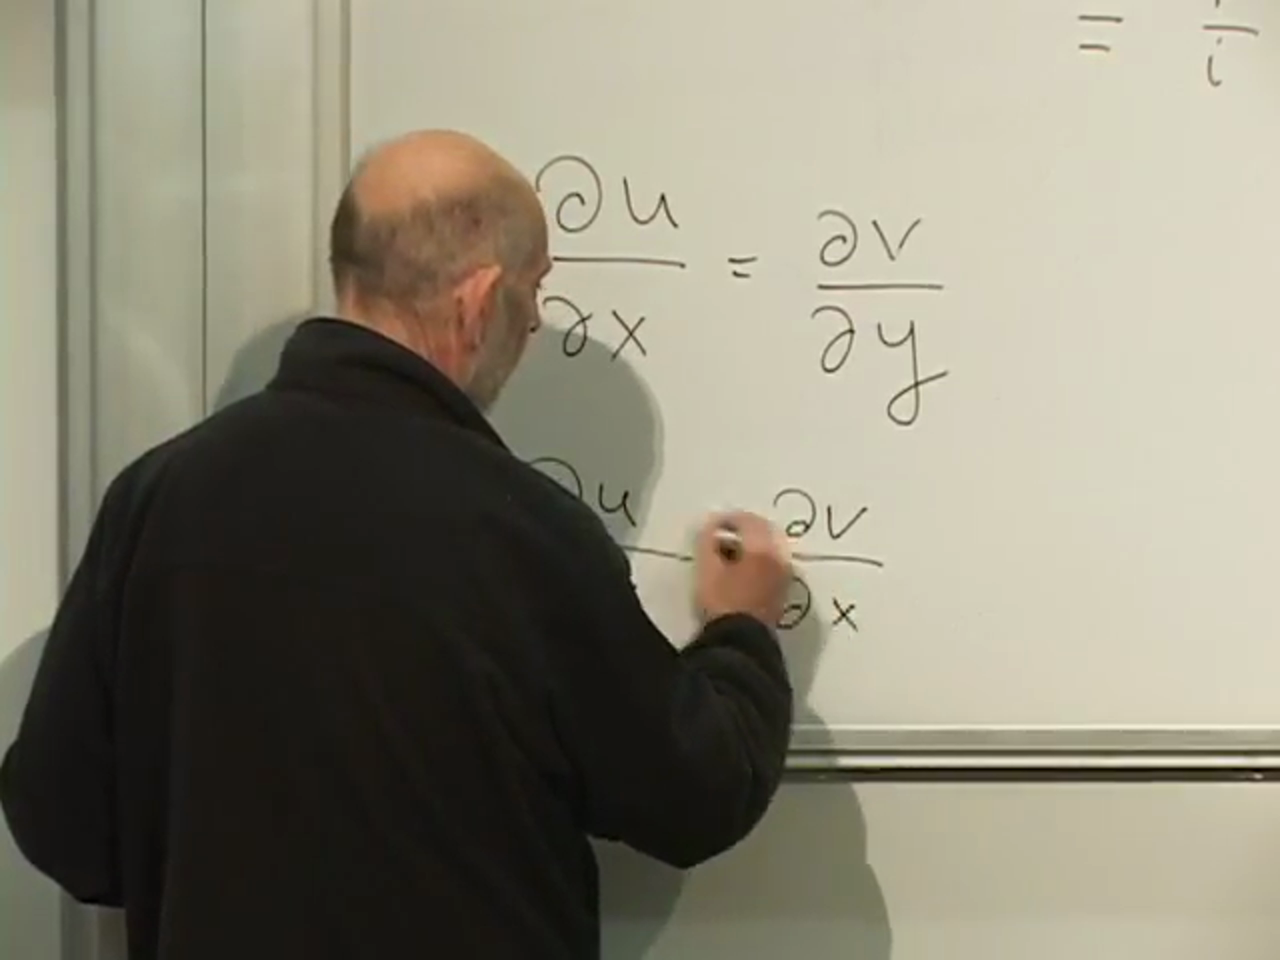
\includegraphics[width=0.70\textwidth]{lecture_08_figure_02.png}
  \caption{完整的柯西--黎曼方程组，包括相对负号。}
  \lectureframe{00:19:48}
  \label{fig:l08-cr-board}
\end{figure}

本讲简要区分了相关术语。在整个有限复平面上全纯的函数称为整函数。亚纯函数可以有孤立极点。因此\(1/z\)在\(z=0\)之外解析，但它不是整函数。

\section{调和共轭与共形几何}

柯西--黎曼方程是一阶耦合方程，但它们蕴含独立的二阶方程。将\(\partial_xu=\partial_yv\)对\(x\)求导，将\(\partial_yu=-\partial_xv\)对\(y\)求导，然后相加：
\begin{align}
  \partial_x^2u&=\partial_x\partial_yv,\\
  \partial_y^2u&=-\partial_y\partial_xv,\\
  \therefore\qquad
  \partial_x^2u+\partial_y^2u&=0.
  \label{eq:l08-harmonic-u}
\end{align}
交换\(u\)与\(v\)重复上述论证，得到
\begin{equation}
  \partial_x^2v+\partial_y^2v=0.
  \label{eq:l08-harmonic-v}
\end{equation}
因此，解析函数的实部和虚部是调和共轭的。两个任意的调和函数并不会自动构成解析函数；它们仍必须由\eqref{eq:l08-cauchy-riemann}相联系。

\begin{figure}[H]
  \centering
  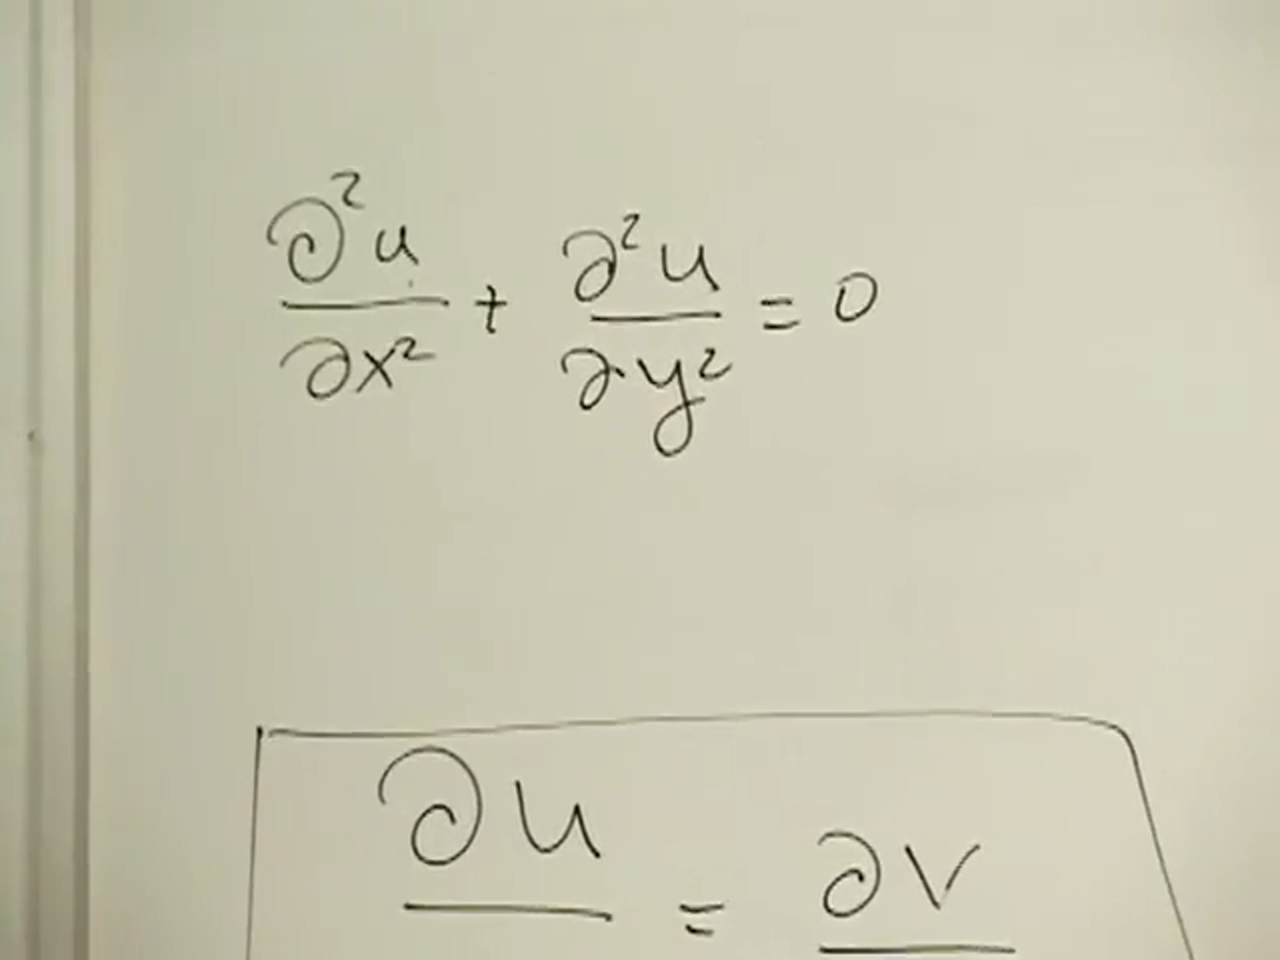
\includegraphics[width=0.68\textwidth]{lecture_08_figure_03.png}
  \caption{混合导数相消，留下解析映射的一个分量所满足的拉普拉斯方程。}
  \lectureframe{00:23:09}
  \label{fig:l08-harmonic-board}
\end{figure}

还有一种有用的矢量解释。若\(\mathbf F=(u,-v)\)，则两个柯西--黎曼方程表明，在所选定向约定下，\(\mathbf F\)的散度和二维旋度均为零。这就是所承诺的回到静电学。

\subsection{为何角度得以保持}

将两个小复位移写成极坐标形式：
\begin{equation}
  \delta z=\rho e^{i\theta},
  \qquad
  \Delta z=\rho'e^{i\theta'}.
\end{equation}
它们的比值具有相位\(\theta-\theta'\)，恰为二者之间的夹角。在解析映射下，
\begin{equation}
  \frac{\delta w}{\delta z}
  =\frac{\Delta w}{\Delta z}
  =w'(z),
\end{equation}
因为导数不依赖于方向。整理可得
\begin{equation}
  \frac{\Delta z}{\delta z}
  =\frac{\Delta w}{\delta w}.
  \label{eq:l08-angle-ratio}
\end{equation}
两边具有相同的相位，因此原区间之间的夹角等于其像之间的夹角。

\begin{figure}[H]
  \centering
  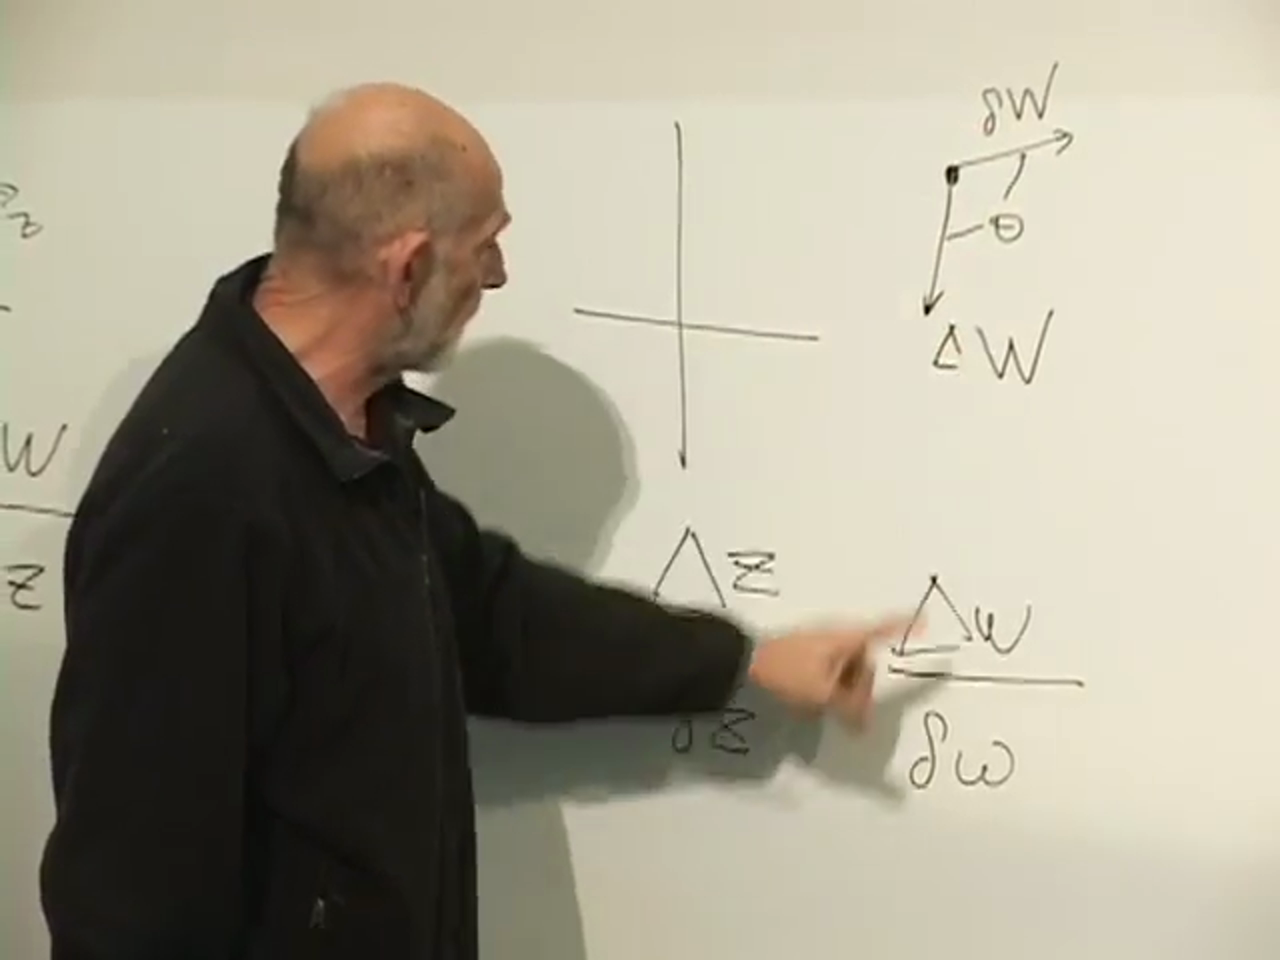
\includegraphics[width=0.70\textwidth]{lecture_08_figure_04.png}
  \medskip

  \begin{tikzpicture}[x=0.9cm,y=0.9cm,>=Latex]
    \begin{scope}
      \draw[->] (-0.2,0) -- (2.3,0);
      \draw[->] (0,-0.2) -- (0,2.1);
      \draw[very thick,blue!65!black,->] (0,0) -- (1.85,0.45)
        node[right] {\(\delta z\)};
      \draw[very thick,orange!75!black,->] (0,0) -- (0.72,1.65)
        node[above] {\(\Delta z\)};
      \draw (0.58,0.14) arc[start angle=14,end angle=66,radius=0.60];
      \node at (1.0,-0.55) {\(z\)-plane};
    \end{scope}
    \draw[->,thick] (3.0,0.9) -- (4.2,0.9)
      node[midway,above] {\(w(z)\)};
    \begin{scope}[xshift=5.0cm]
      \draw[->] (-0.2,0) -- (2.3,0);
      \draw[->] (0,-0.2) -- (0,2.1);
      \draw[very thick,blue!65!black,->] (0,0) -- (1.65,0.70)
        node[right] {\(\delta w\)};
      \draw[very thick,orange!75!black,->] (0,0) -- (0.48,1.62)
        node[above] {\(\Delta w\)};
      \draw (0.54,0.23) arc[start angle=23,end angle=74,radius=0.59];
      \node at (1.0,-0.55) {\(w\)-plane};
    \end{scope}
  \end{tikzpicture}
  \caption{黑板证明与一个清晰的局部重构。乘以\(w'(z)\)会将每个无穷小方向旋转并重新缩放相同的量，从而保持它们的相对角度。}
  \lectureframe{00:34:11}
  \label{fig:l08-angle-proof}
\end{figure}

这一局部论证假设\(w'(z)\neq0\)。在临界点处，映射可能不再是局部一一的，必须单独处理其几何。远离此类点处，解析映射与保向共形映射在局部是同一类对象。

\section{训练眼力的例子}

\subsection{平方映射与复共轭}

对于\(w=z^2\)，
\begin{equation}
  (x+iy)^2=x^2-y^2+2ixy=u+iv,
\end{equation}
因此
\begin{equation}
  u=x^2-y^2,
  \qquad
  v=2xy.
  \label{eq:l08-z-squared-components}
\end{equation}
\(u\)的二阶导数为\(2\)和\(-2\)；\(v\)的二阶导数分别消失。二者都是调和的，直接求导也验证了柯西--黎曼方程。

\begin{figure}[H]
  \centering
  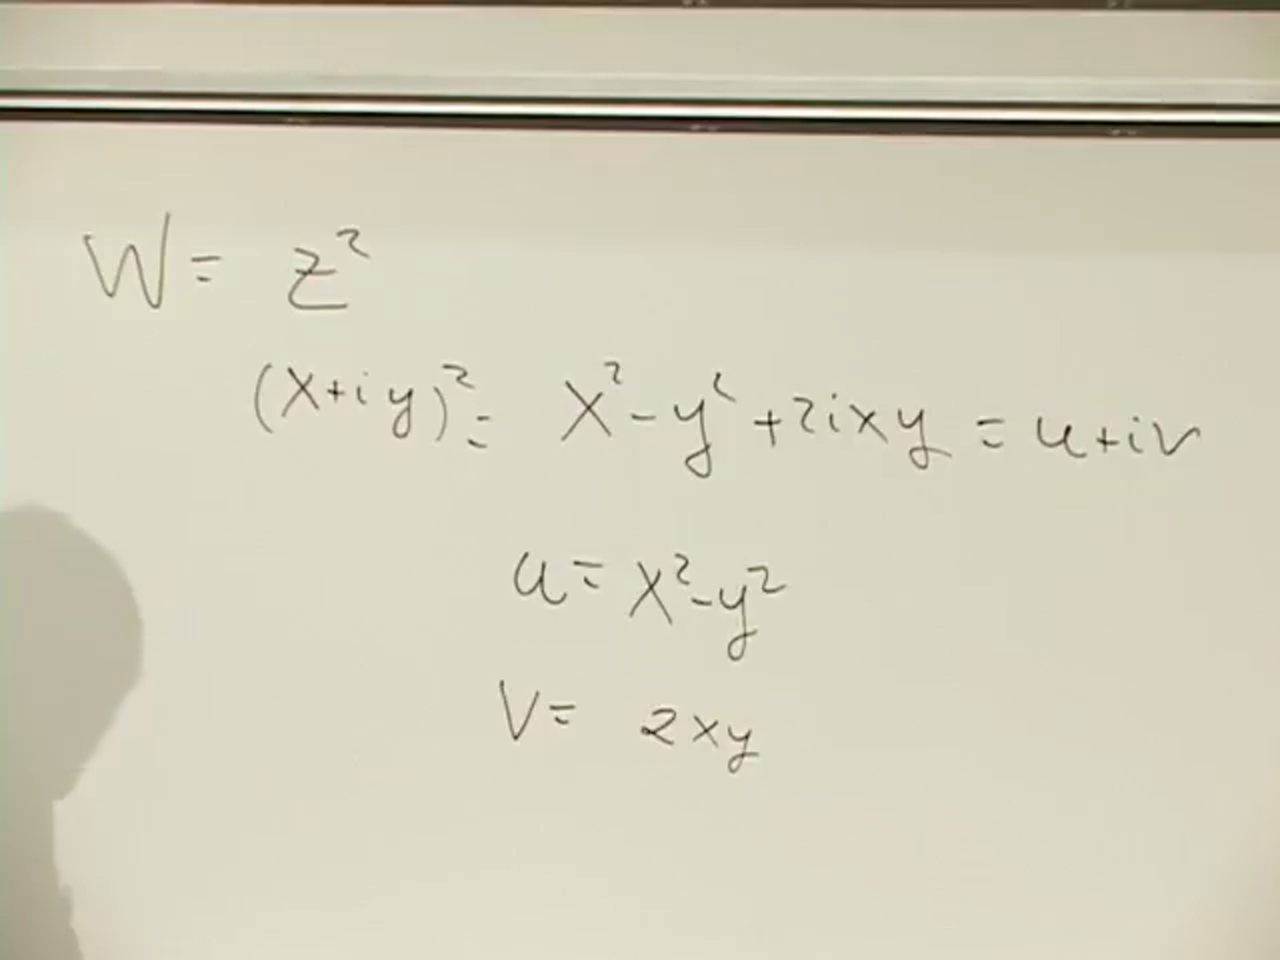
\includegraphics[width=0.72\textwidth]{lecture_08_figure_05.png}
  \caption{平方映射分解为其实部和虚部调和分量。}
  \lectureframe{00:36:45}
  \label{fig:l08-z-square-board}
\end{figure}

\begin{classroomqa}
\audiencequestion{\(1/z\)是否给出一个非解析的例子？
\lecturetimestamp{00:37:49}}
\lecturerresponse{仅在一个点处。它在\(z\neq0\)处解析，并在原点有一个极点。要看到一个处处不满足柯西--黎曼检验的映射，复共轭是更好的例子。}
\end{classroomqa}

相比之下，
\begin{equation}
  w=\bar z=x-iy
  \qquad\Longrightarrow\qquad
  u=x,\quad v=-y
\end{equation}
反转定向。它的导数以符号之差违反第一个柯西--黎曼方程，因此作为\(z\)的函数它不是解析的。

\begin{figure}[H]
  \centering
  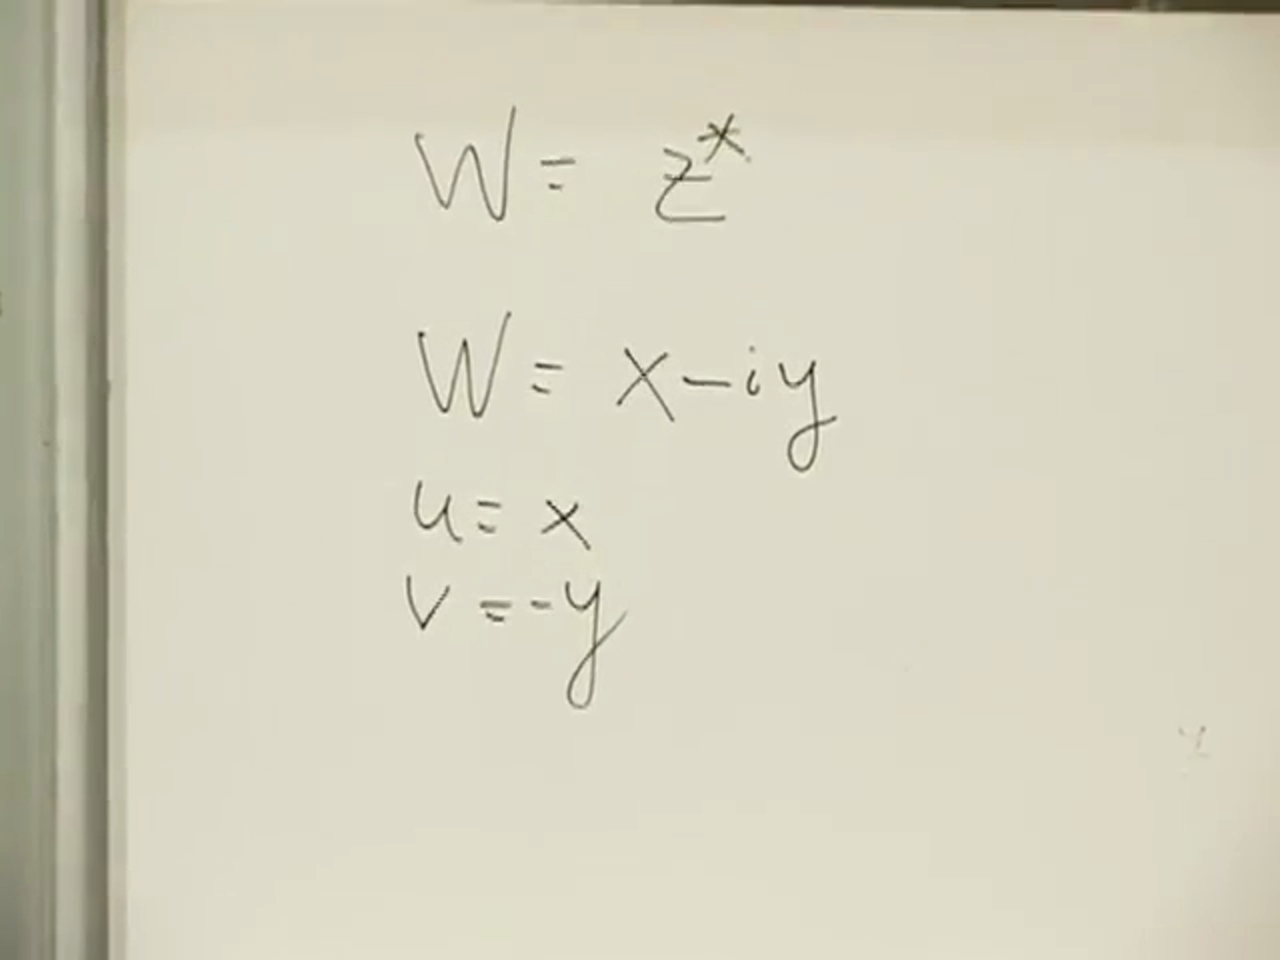
\includegraphics[width=0.62\textwidth]{lecture_08_figure_06.png}
  \caption{复共轭提供了刻意构造的非解析反例。}
  \lectureframe{00:38:38}
  \label{fig:l08-conjugate-board}
\end{figure}

\subsection{指数函数及其反函数}

\begin{classroomqa}
\audiencequestion{若\(e^z\)是解析的，为何其反函数\(\log z\)也应是解析的？\lecturetimestamp{00:40:38}}
\lecturerresponse{在反函数存在且\(w'(z)\neq0\)处，其导数为\(1/w'(z)\)。因此方向无关性得以保持。整体上对数函数是多值的，因此需选择一个分支并排除其分支点和割线。局部共形陈述在该选定区域上仍然成立。}
\end{classroomqa}

欧拉公式给出
\begin{equation}
  w=e^z=e^{x+iy}
  =e^x(\cos y+i\sin y),
\end{equation}
因此
\begin{equation}
  u=e^x\cos y,
  \qquad
  v=e^x\sin y.
  \label{eq:l08-exponential-components}
\end{equation}
例如，\(\partial_xu=e^x\cos y=\partial_yv\)，第二个柯西--黎曼方程同样直接可得。

\begin{figure}[H]
  \centering
  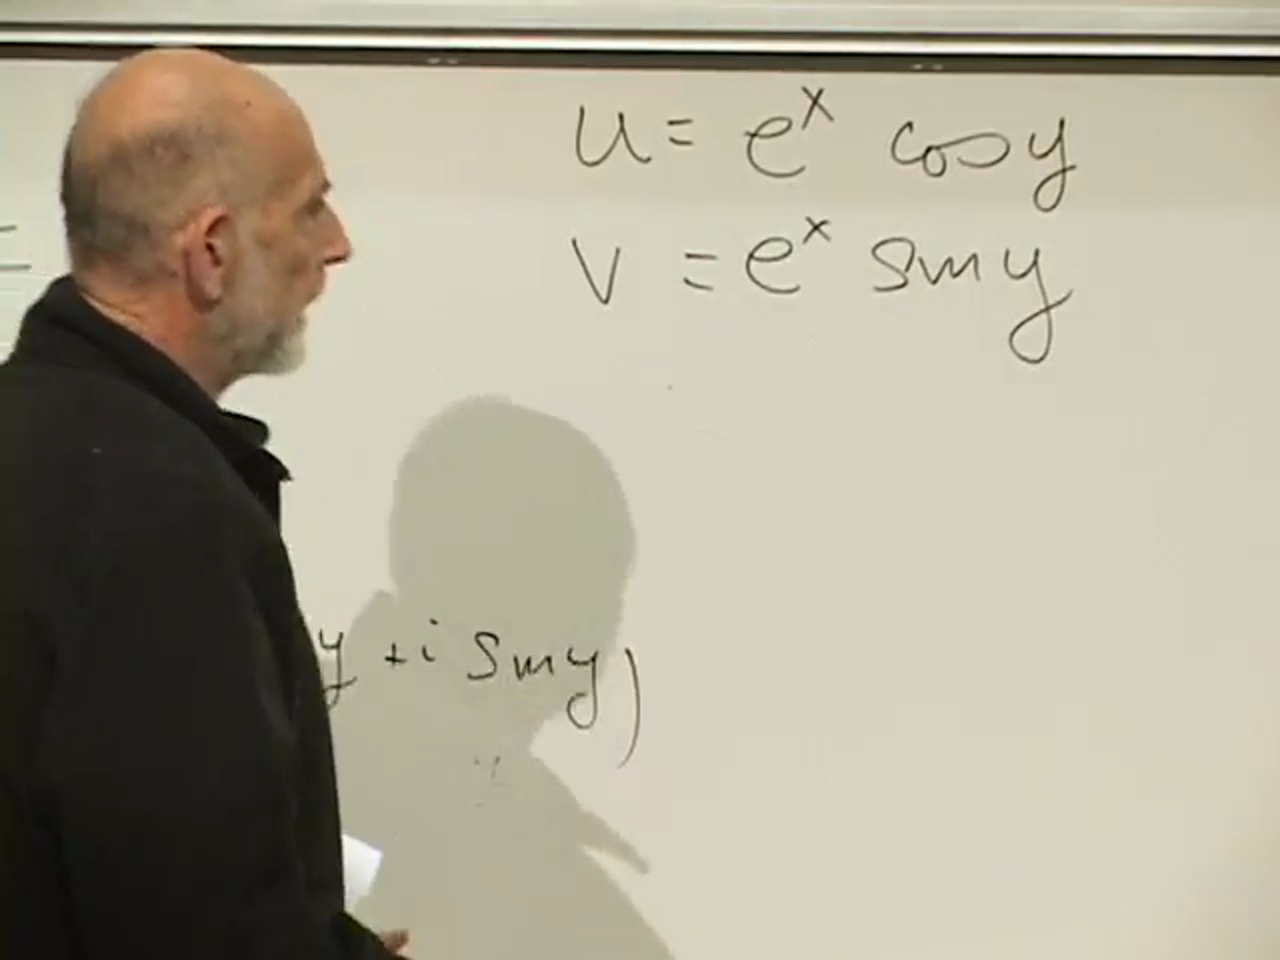
\includegraphics[width=0.68\textwidth]{lecture_08_figure_07.png}
  \caption{指数映射的实部和虚部分量。}
  \lectureframe{00:42:23}
  \label{fig:l08-exponential-board}
\end{figure}

\section{半平面、带形、柱面与圆盘}

\subsection{对数将半径变为时间}

取右半平面，其中\(-\pi/2<\theta<\pi/2\)，并写出
\begin{equation}
  z=re^{i\theta},
  \qquad
  w=\log z=\log r+i\theta.
  \label{eq:l08-log-map}
\end{equation}
该半平面映射到无限带形
\begin{equation}
  -\frac{\pi}{2}<\operatorname{Im}w<\frac{\pi}{2}.
\end{equation}
固定\(\theta\)的射线变为水平线，而固定\(r\)的半圆变为竖直线。原点被送到\(\operatorname{Re}w=-\infty\)，而\(r=\infty\)被送到\(\operatorname{Re}w=+\infty\)。

\begin{figure}[H]
  \centering
  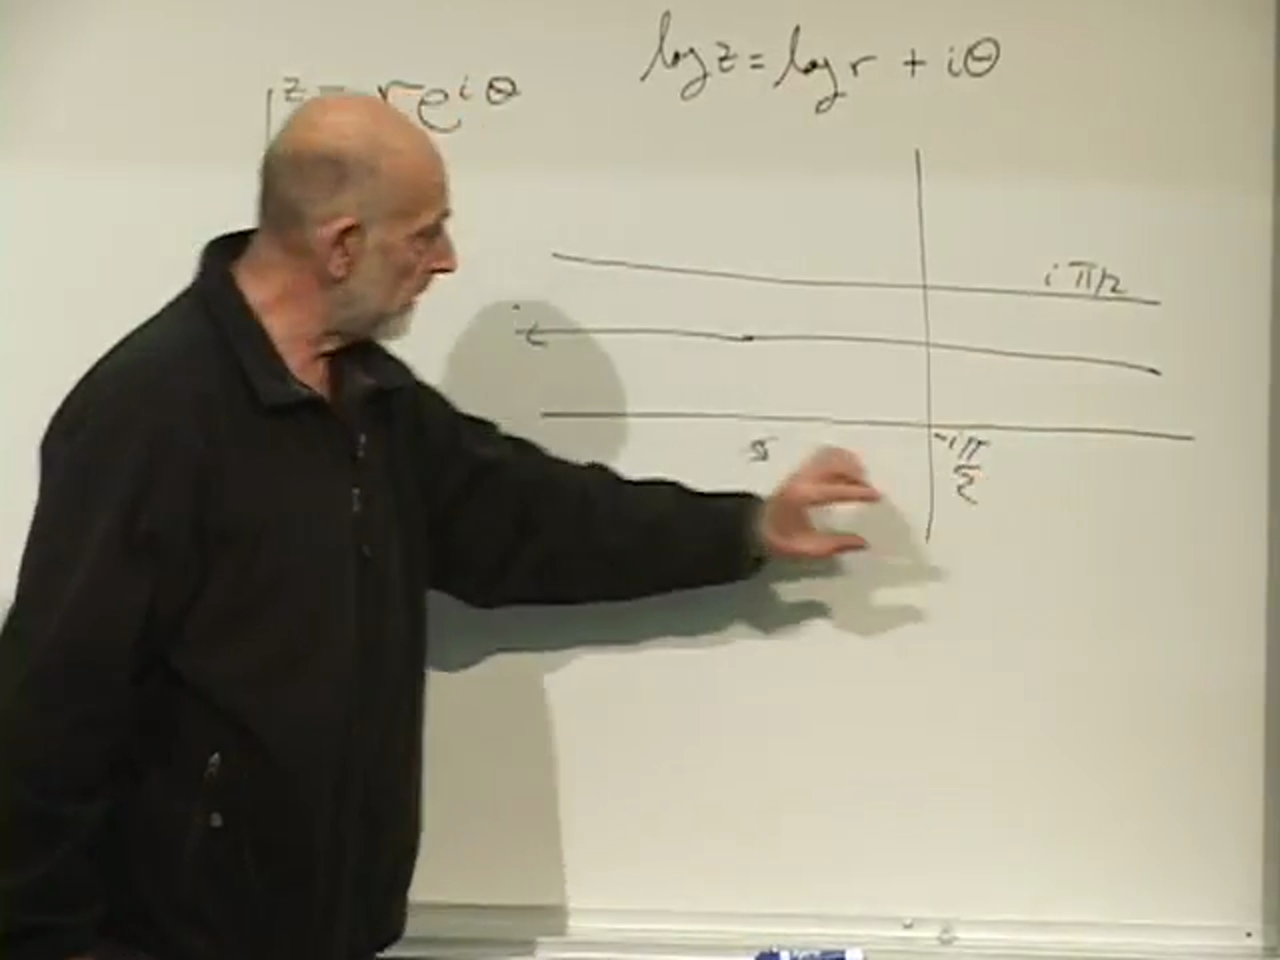
\includegraphics[width=0.75\textwidth]{lecture_08_figure_08.png}
  \caption{对数将右半平面映入一个无限带形：极坐标射线与半圆变为正交的矩形网格。}
  \lectureframe{00:47:48}
  \label{fig:l08-log-strip-board}
\end{figure}

这条带子是开弦的标准世界面。它有界的坐标是沿弦的参数，而沿无界方向的平移则是世界面时间。在逆指数映射下，时间平移变为伸缩\(z\mapsto e^a z\)。因此，同一个对称性在带子上看起来是平移，而在半平面上看起来是均匀膨胀。

\begin{classroomqa}
\audiencequestion{像\(r=1\)这样的特定值会到哪里去，带子上的坐标仍然是极坐标吗？\lecturetimestamp{00:50:58}}
\lecturerresponse{固定半径的圆变成\(\operatorname{Re}w=\log r\)处的竖直线；特别地，\(r=1\)映射到中心线\(\operatorname{Re}w=0\)。极坐标描述\(z\)平面。\(w\)平面使用普通的直角坐标\((\log r,\theta)\)。}
\end{classroomqa}

如果整个去心平面被\(\log z\)映射，则角坐标的周期为\(2\pi\)。因此，所得的带子的上下边缘被等同起来：它是一个无限长圆柱面。带边界的半平面描述开弦世界面；没有边界且角度具有周期性的整个平面描述闭弦圆柱面。

\begin{figure}[H]
  \centering
  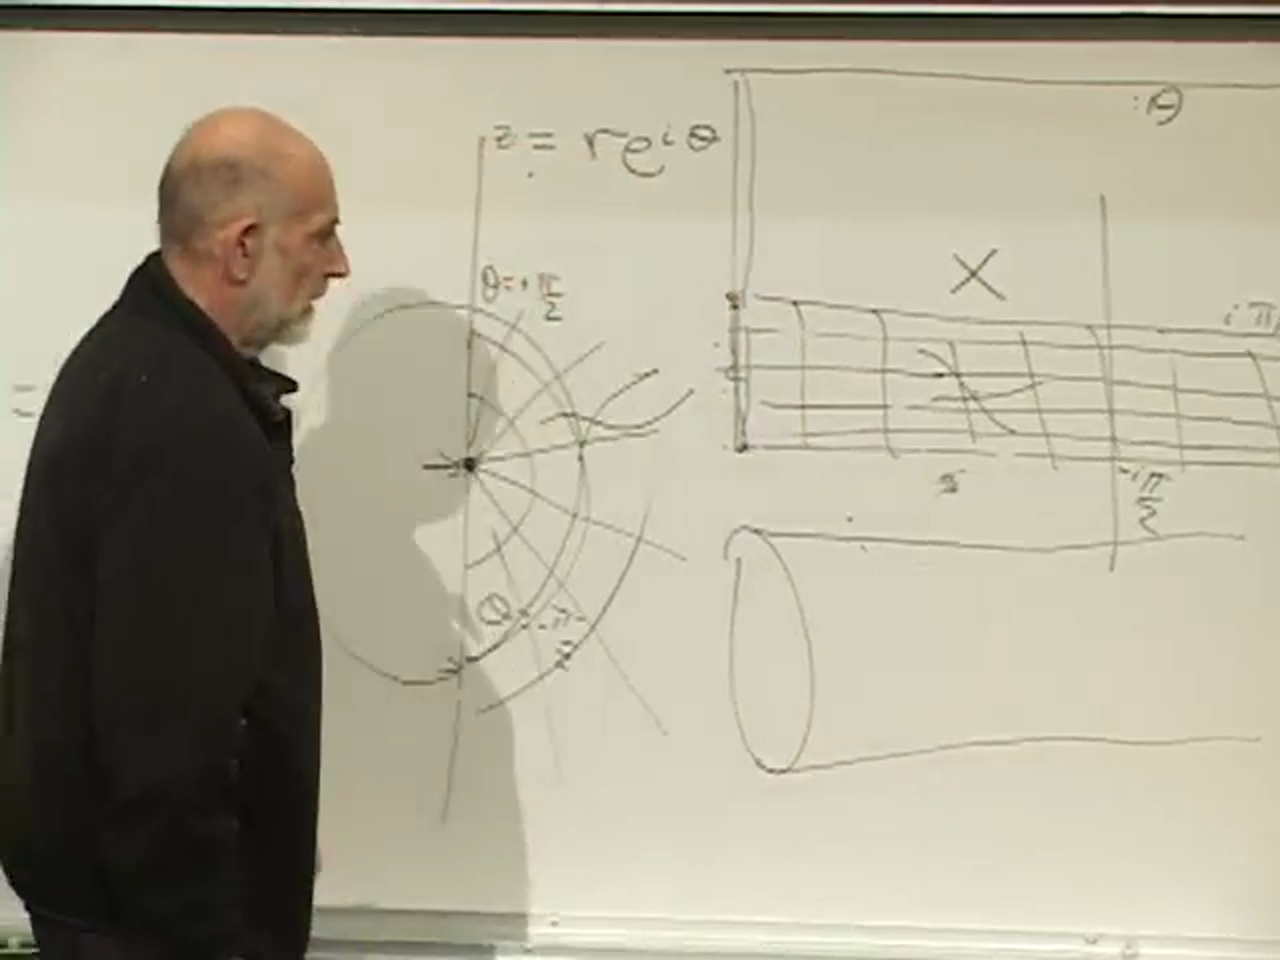
\includegraphics[width=0.75\textwidth]{lecture_08_figure_09.png}
  \caption{半平面/带子图像，以及将整个去心平面变成闭弦圆柱面的周期性等同。}
  \lectureframe{00:54:23}
  \label{fig:l08-open-closed-board}
\end{figure}

\subsection{到单位圆盘的Cayley映射}

线性分式映射，或称Möbius映射，将右半平面映到单位圆盘：
\begin{equation}
  w=\frac{z-1}{z+1}.
  \label{eq:l08-cayley}
\end{equation}
它将\(z=0\)映到\(-1\)，将\(z=\infty\)映到\(+1\)，并将虚轴映到\(|w|=1\)。如果\(z=ir\)，
\begin{equation}
  \left|\frac{ir-1}{ir+1}\right|=1.
\end{equation}
满足\(\operatorname{Re}z>0\)的点位于圆内；左半平面映到圆外。
\editorialnote{在实际推导过程中，当描述圆盘内部的像时，写下了倒数\((z+1)/(z-1)\)。该倒数具有相同的单位圆边界，但将右半平面映到外部。方程\eqref{eq:l08-cayley}是与所述几何相一致的圆盘内部约定。}

\begin{figure}[H]
  \centering
  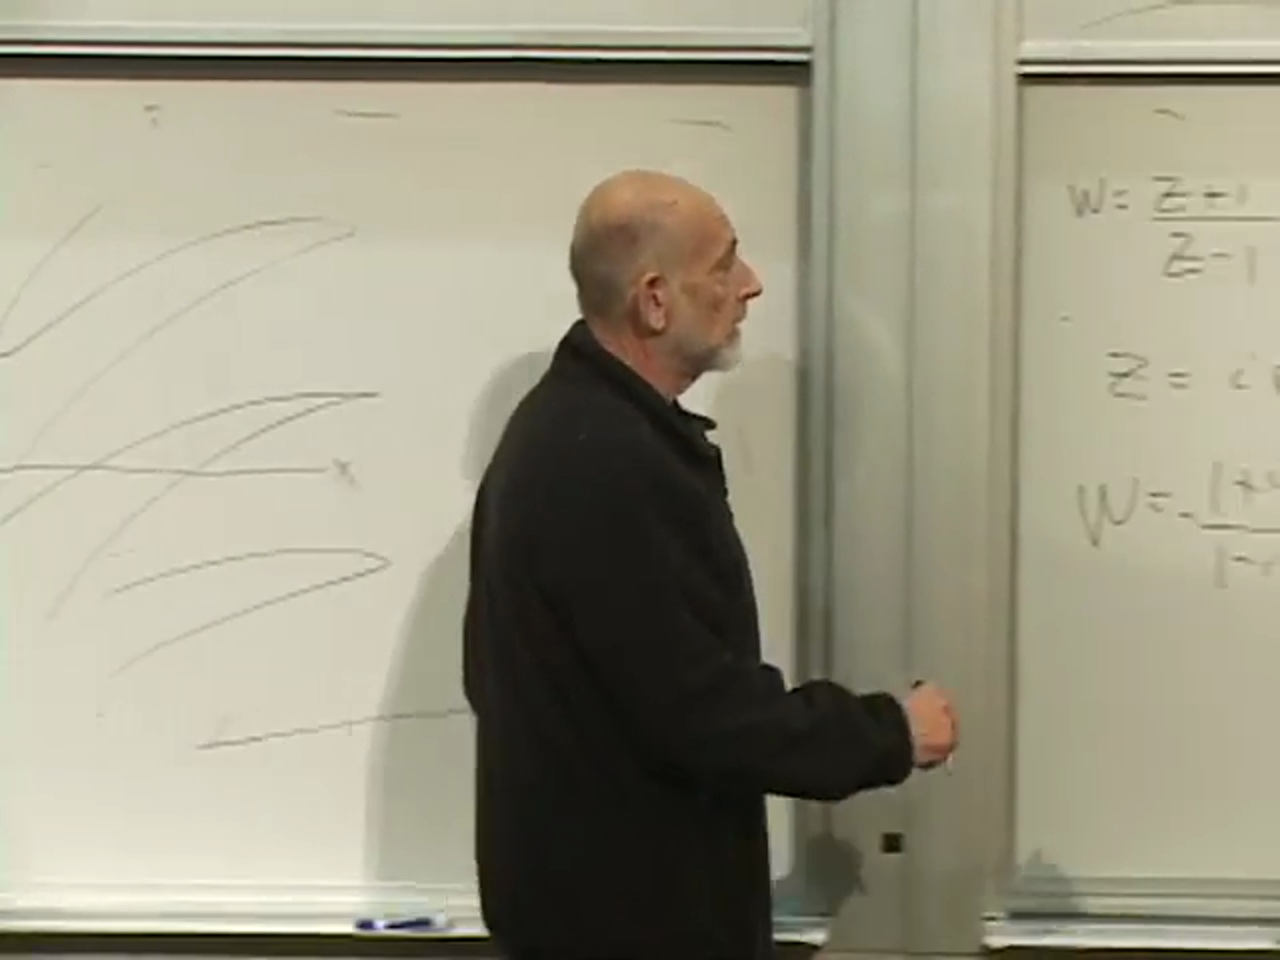
\includegraphics[width=0.72\textwidth]{lecture_08_figure_10.png}
  \caption{单位圆边界的线性分式构造。黑板上可见的倒数约定交换了内部与外部。}
  \lectureframe{00:58:38}
  \label{fig:l08-cayley-board}
\end{figure}

Möbius映射将圆和直线的广义集合映为圆和直线。因此，半平面上的径向和圆周网格在圆盘上变成两族正交的弧。直线直径不过是圆心趋于无穷远的圆的极限情形。

\begin{classroomqa}
\audiencequestion{在圆盘内部画出的弧真的是圆吗？\lecturetimestamp{01:00:55}}
\lecturerresponse{是的。它们的圆心位于不同位置，常常在可见圆盘之外。直径是同一族中半径趋于无穷的极限。}
\end{classroomqa}

\begin{classroomqa}
\audiencequestion{圆盘的图是否意味着它是一个球面，另一个半平面到哪里去了？\lecturetimestamp{01:01:21}}
\lecturerresponse{这里的图是一个平直的圆盘，不是球面。右半平面映到其边界内部，左半平面映到外部。如果向整个复平面添加无穷远点，那么该扩充平面可以通过球极投影表示为球面；那是一个不同的整体陈述。}
\end{classroomqa}

\begin{classroomqa}
\audiencequestion{哪些圆盘曲线对应于原来的径向辐条和固定半径的半圆？\lecturetimestamp{01:02:59}}
\lecturerresponse{正实轴变成连接\(-1\)和\(+1\)的直径。其他射线变成连接同样这些边界点的圆弧。固定半径的半圆变成在单位圆上开始并结束的正交族。}
\end{classroomqa}

\begin{figure}[H]
  \centering
  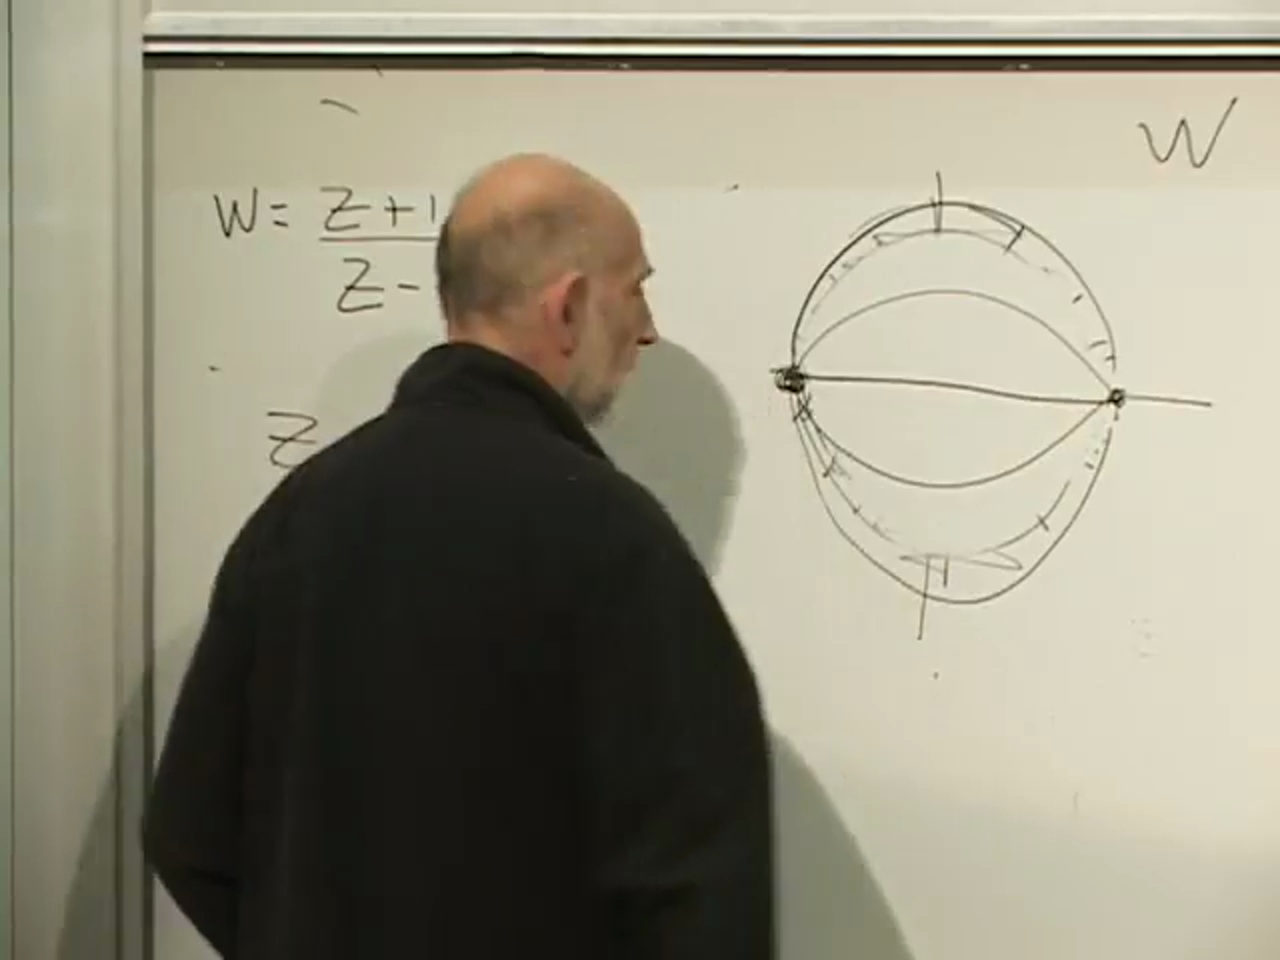
\includegraphics[width=0.72\textwidth]{lecture_08_figure_11.png}
  \caption{半平面中的直线和半圆变成圆盘中的正交圆与直线族。}
  \lectureframe{01:03:48}
  \label{fig:l08-circle-grid-board}
\end{figure}

\section{四弦世界面}

现在我们可以回到散射。两条开弦进入，结合成一条弦，传播任意一段时间，然后分裂成两条出射弦。在带子坐标中，世界面看起来像一条长带子，从两端各有一条缝---这就是“运动绷带”图像。中间寿命不是预先选定的。它是振幅所积分的诸多历史之一。

设\((\sigma,\tau)\)为世界面上的坐标，并设
\begin{equation}
  X^\mu=X^\mu(\sigma,\tau)
  \label{eq:l08-embedding}
\end{equation}
给出它在时空中的位置。标签\(\sigma,\tau\)位于二维参数曲面上；指标\(\mu\)标记时空坐标。在玻色弦理论中\(\mu=0,\ldots,25\)；在超弦情形中有十个时空坐标。

经过 Wick 转动后，自由嵌入场具有欧几里得作用量
\begin{equation}
  S_E[X]
  =\frac{1}{4\pi\alpha'}\int_\Sigma d\sigma\,d\tau\,
  \left[
    \partial_\tau X^\mu\partial_\tau X_\mu
    +\partial_\sigma X^\mu\partial_\sigma X_\mu
  \right].
  \label{eq:l08-euclidean-action}
\end{equation}
相应的路径积分对所选世界面到时空的每一个嵌入求和：
\begin{equation}
  \int\mathcal D X\,e^{-S_E[X]}.
  \label{eq:l08-bare-worldsheet-integral}
\end{equation}

\begin{figure}[H]
  \centering
  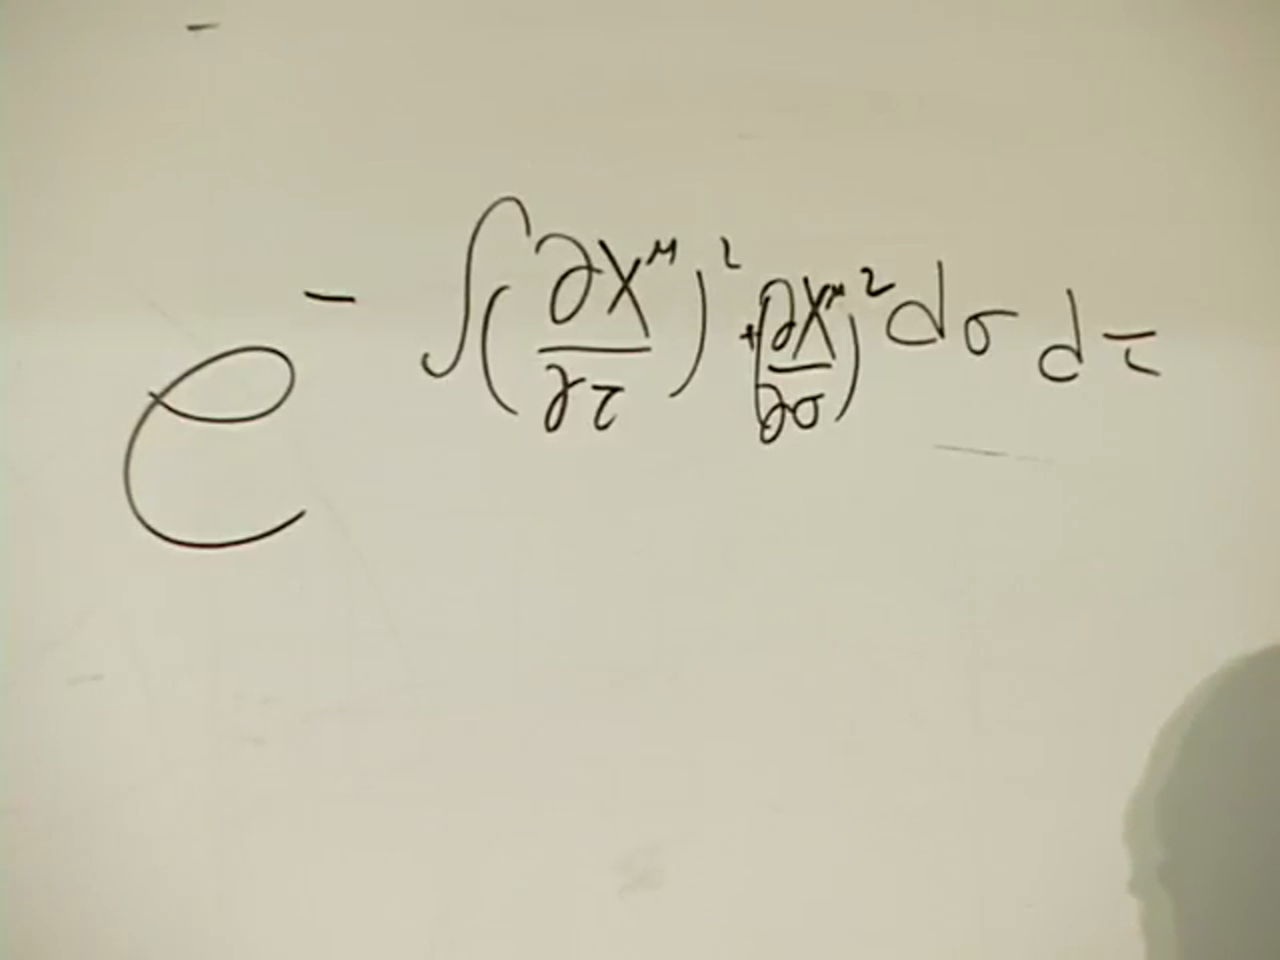
\includegraphics[width=0.74\textwidth]{lecture_08_figure_12.png}
  \caption{完整的正欧几里得世界面权重。两个导数项对所有时空分量求和。}
  \lectureframe{01:11:34}
  \label{fig:l08-action-board}
\end{figure}

带缝长条只有一个连通边界。因此，共形自由度允许将它表示为一个圆盘。长条的四个远端成为边界上的四个标记点。形变这些标记点会改变长条坐标中连接与分裂之间的表观间隔，但不会改变底层的曲面或物理。

\begin{figure}[H]
  \centering
  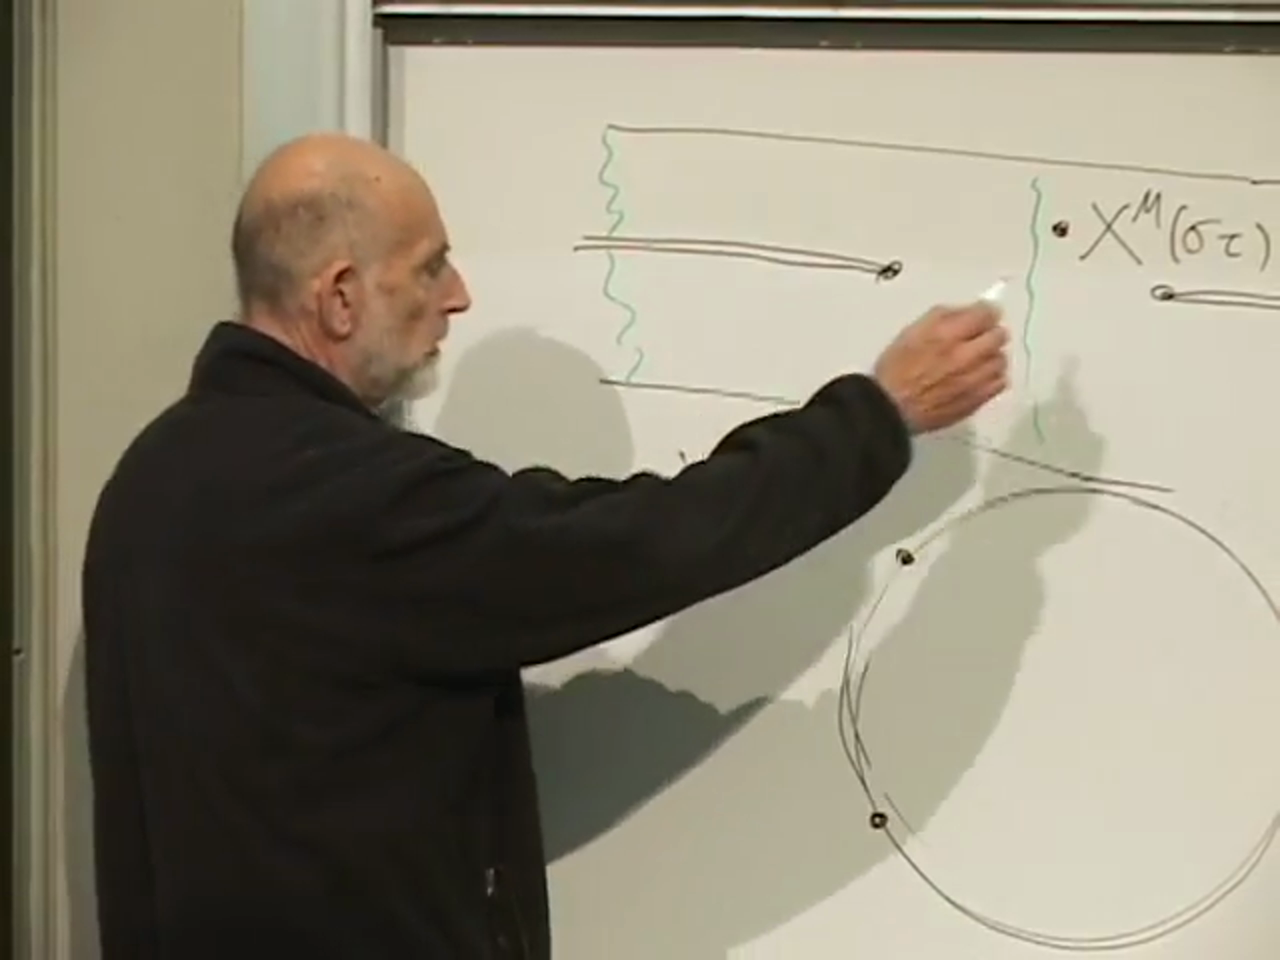
\includegraphics[width=0.76\textwidth]{lecture_08_figure_13.png}
  \caption{带缝长条世界面及其圆盘表示，边界点对应外部弦。}
  \lectureframe{01:15:18}
  \label{fig:l08-bandage-disc-board}
\end{figure}

用来描绘这个共形映射的详细网格线不携带任何物理内容。重要的是拓扑、边界以及标记的外部点。同一个世界面可以被拉伸成不同的通道图像，而不会引入新的相互作用。

\section{外部态作为边界插入}

裸积分 \eqref{eq:l08-bare-worldsheet-integral} 尚未说明哪些动量进入、哪些动量离开。对于动量为 \(k_i^\mu\) 的标量开弦态，在边界上插入顶点算符
\begin{equation}
  V_i(z_i)=e^{\,i k_i\cdot X(z_i)},
  \qquad
  k_i\cdot X=k_{i\mu}X^\mu.
  \label{eq:l08-vertex}
\end{equation}
点 \(z_i\) 是世界面边界上的一个位置。它不是时空坐标，也不是动量的方向。

\begin{figure}[H]
  \centering
  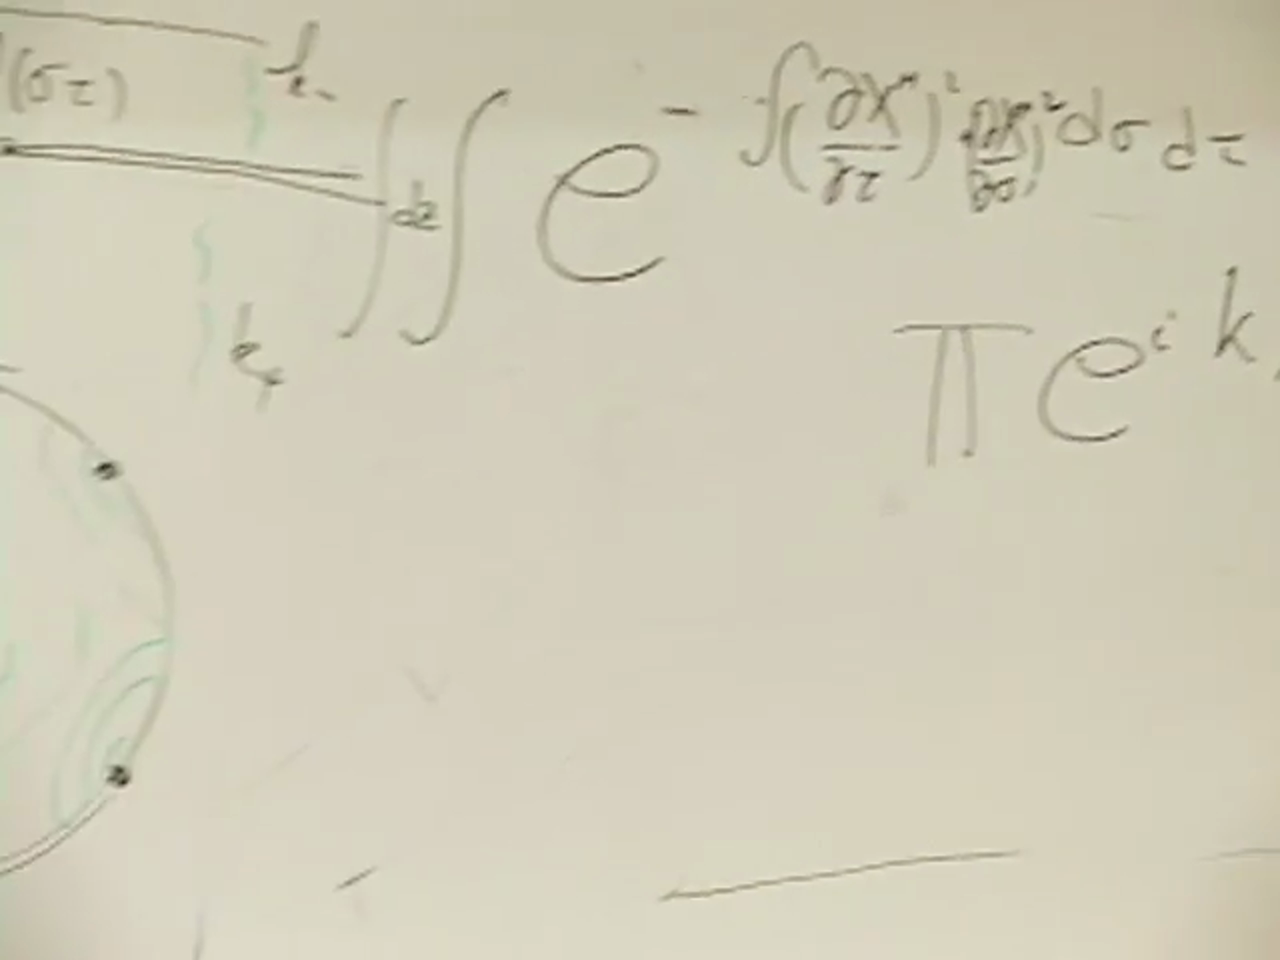
\includegraphics[width=0.72\textwidth]{lecture_08_figure_14.png}
  \caption{体欧几里得权重与边界动量插入的乘积被显示为不同的因子。}
  \lectureframe{01:18:58}
  \label{fig:l08-vertex-board}
\end{figure}

对于 \(n\) 条外部开弦，示意性的规定是
\begin{equation}
  \begin{aligned}
    \mathcal A_n(k_1,\ldots,k_n)
    &=\int_{\mathcal M_{0,n}^{\partial}}\!d\mu(z_i)
      \int\mathcal D X\\
    &\quad\times e^{-S_E[X]}
      \prod_{i=1}^{n}e^{\,i k_i\cdot X(z_i)}.
  \end{aligned}
  \label{eq:l08-open-string-prescription}
\end{equation}
泛函积分是对嵌入 \(X^\mu\) 进行的。有限维积分是对不等价的边界插入位置进行的。极化因子和规范固定测度在此阶段被省略，正如讲座中那样。
\editorialnote{一个完整的规范固定弦振幅还包含相应的鬼场贡献、依赖于态的顶点因子、耦合常数和归一化。方程
\eqref{eq:l08-open-string-prescription} 记录了本讲座中展开的嵌入场依赖和位置依赖。}

\begin{classroomqa}
\audiencequestion{如果外部动量是固定的，为什么还要对它们积分？\lecturetimestamp{01:20:42}}
\lecturerresponse{它们并没有被积分。\(k_i\) 是散射振幅的固定标记。被积分的是嵌入场以及那些固定动量所插入的世界面位置 \(z_i\)。后一个积分取代了长条图像中对中间寿命的积分。}
\end{classroomqa}

\begin{classroomqa}
\audiencequestion{顶点因子的乘积是在路径积分内部，它是作用量的一部分吗？\lecturetimestamp{01:21:39}}
\lecturerresponse{它是在泛函积分内部乘在 \(e^{-S_E}\) 上。也可以等价地将这些因子指数化，并把它们视为加到作用量上的局域源项，但它们在概念上是顶点算符，而不是自由体作用量的一部分。}
\end{classroomqa}

\begin{figure}[H]
  \centering
  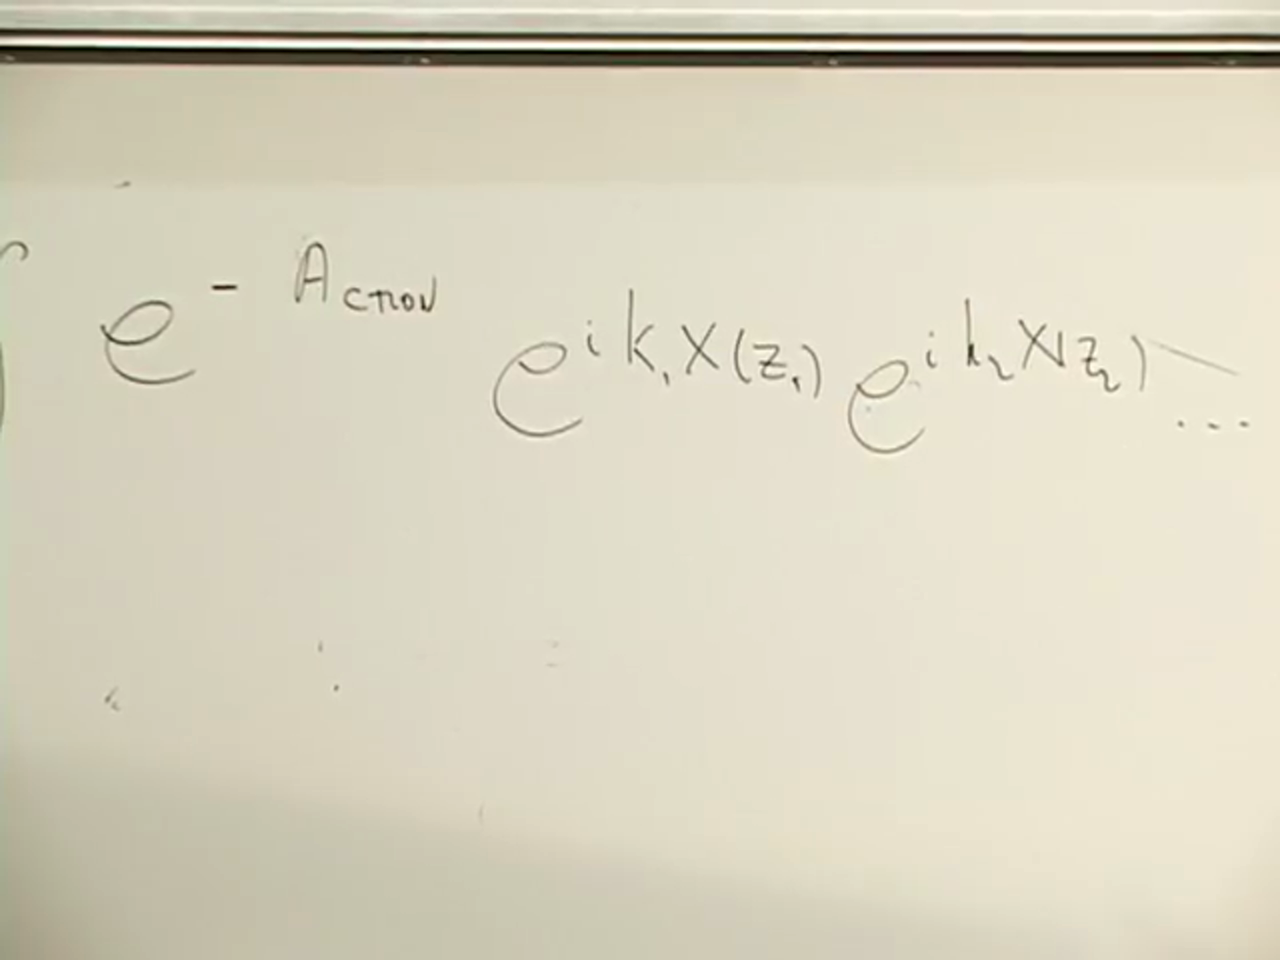
\includegraphics[width=0.76\textwidth]{lecture_08_figure_15.png}
  \caption{用分离的因子 \(e^{ik_i\cdot X(z_i)}\) 表示相继外部粒子的路径积分。}
  \lectureframe{01:23:23}
  \label{fig:l08-full-prescription-board}
\end{figure}

\begin{classroomqa}
\audiencequestion{为什么在世界面 Wick 转动之后 \(e^{ik\cdot X}\) 仍然含有 \(i\)？\lecturetimestamp{01:23:42}}
\lecturerresponse{该转动改变了世界面时间，并将体权重从 \(e^{iS}\) 转换为 \(e^{-S_E}\)。动量本征函数中的 \(i\) 是标记时空动量的傅里叶相位。它起着不同的作用，并且保留下来。}
\end{classroomqa}

\begin{classroomqa}
\audiencequestion{位置 \(z_i\) 是否决定动量矢量的方向？\lecturetimestamp{01:24:19}}
\lecturerresponse{不决定。方向编码在时空分量 \(k_i^\mu\) 中。插入点 \(z_i\) 说明该动量从何处进入世界面描述；\(X^\mu(z_i)\) 是 \(\mathcal D X\) 所求和的对象之一。}
\end{classroomqa}

\begin{classroomqa}
\audiencequestion{所画的绷带腿的角度是否编码了物理动量的方向？\lecturetimestamp{01:25:07}}
\lecturerresponse{不编码。绷带是参数空间，不是弦在物理时空中的图像。它的腿可以画成水平的、倾斜的或共形弯曲的。物理方向由分量 \(k^\mu\) 承载，而 \(X^\mu(\sigma,\tau)\) 则被积分掉。}
\end{classroomqa}

\section{作为静电学的高斯积分}

作用量\eqref{eq:l08-euclidean-action}对每个分量\(X^\mu\)都是二次的，而一旦把插入算符的指数与作用量合并，这些插入就表现为线性源。因此泛函积分是高斯型的。在其鞍点处，每个时空分量都满足一个示意形式为
\begin{equation}
  \nabla^2 X^\mu(z)
  \propto
  i\alpha'\sum_i k_i^\mu\,\delta(z-z_i),
  \label{eq:l08-electrostatic-source}
\end{equation}
的泊松方程，并带有圆盘边缘上的开弦边界条件。每个\(X^\mu\)的行为都像一个独立的静电势，而每个动量分量\(k_i^\mu\)的行为则像置于\(z_i\)处的相应电荷。

\begin{figure}[H]
  \centering
  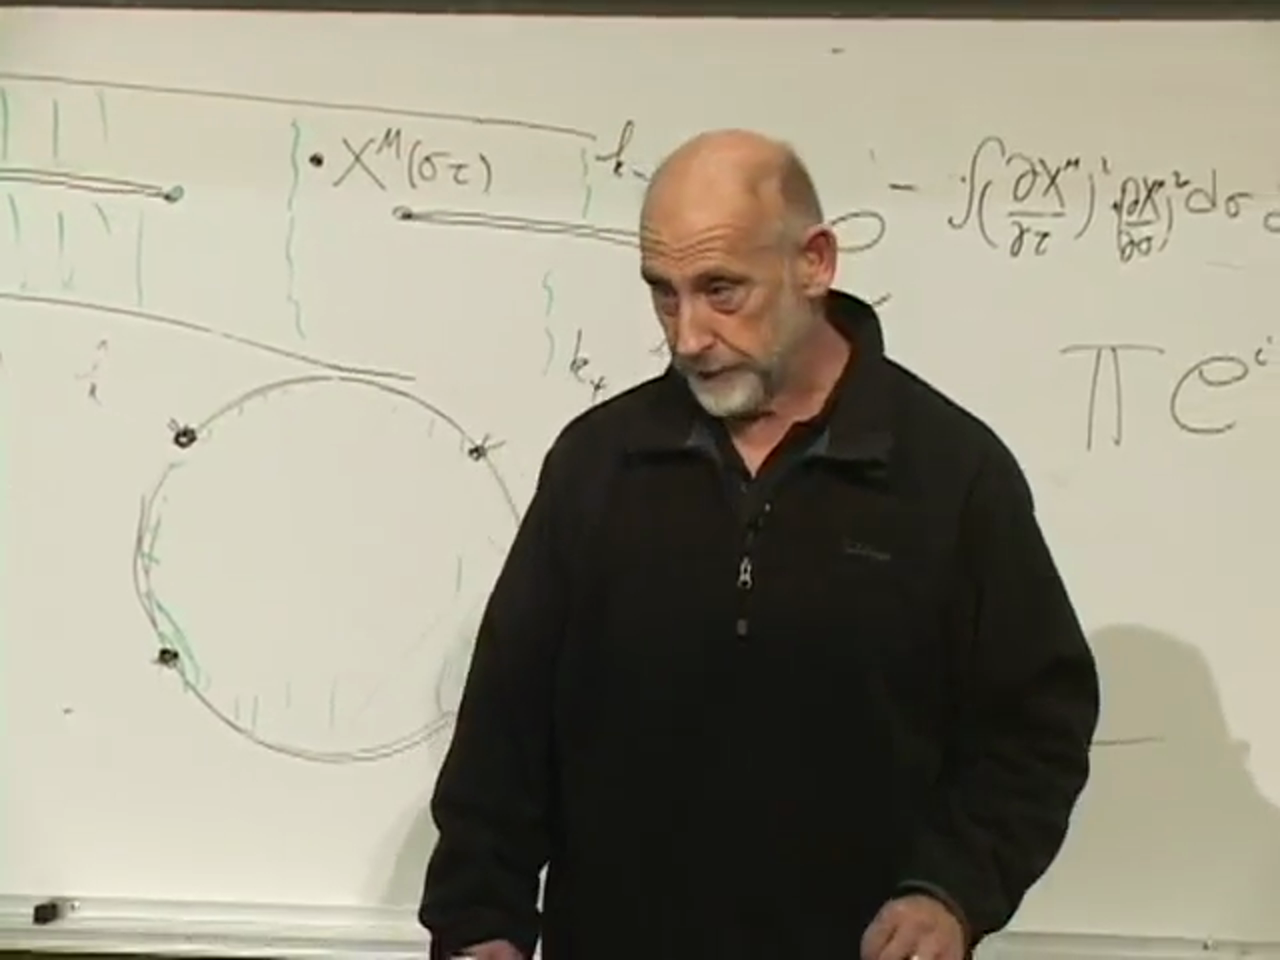
\includegraphics[width=0.76\textwidth]{lecture_08_figure_16.png}
  \caption{带有边界源的圆盘被解释为：对每个时空分量各有一个独立的二维静电场问题。}
  \lectureframe{01:28:58}
  \label{fig:l08-electrostatic-disc-board}
\end{figure}

求解该静电场问题，计算其能量，对负能量取指数，最后对不等价的电荷位置积分。在标准的开弦归一化下，嵌入场关联函数给出 Koba--Nielsen 因子
\begin{equation}
  \left\langle\prod_i e^{\,ik_i\cdot X(z_i)}\right\rangle
  \propto
  (2\pi)^D\delta^{(D)}\!\left(\sum_i k_i\right)
  \prod_{i<j}|z_i-z_j|^{2\alpha' k_i\cdot k_j}.
  \label{eq:l08-koba-nielsen}
\end{equation}
该 delta 函数表示动量守恒。乘积中包含静电场成对能量。对于此处所用的四个标量边界插入，固定三个位置后，剩余积分就化为前几讲中遇到的 Euler beta 积分。

\begin{classroomqa}
\audiencequestion{是有二十六个静电能，还是只有一个？
\lecturetimestamp{01:30:53}}
\lecturerresponse{对每个时空分量，都有一个独立的势和场。在一个正交归一的靶空间基中，它们的二次能量没有交叉项，并且这些贡献在取指数之前被加到一个总作用量中。}
\end{classroomqa}

\begin{classroomqa}
\audiencequestion{圆盘的角坐标就是物理散射角吗？\lecturetimestamp{01:32:10}}
\lecturerresponse{不是。它是一个世界面位置参数。它的不等价组合与中间传播间隔有关，并且要被积分掉。物理散射角通过由固定动量构造的 Lorentz 不变量来编码。}
\end{classroomqa}

\begin{classroomqa}
\audiencequestion{为什么这一构造在临界维数之外会失效？
\lecturetimestamp{01:32:35}}
\lecturerresponse{仅靠形式上的高斯积分并不是全部一致性条件。规范固定会引入一个共形反常，其物质贡献与鬼场贡献只有在临界维数下才会相消：玻色弦为\(D=26\)，超弦为\(D=10\)。若没有这种相消，量子世界面所假定的共形对称性就会丧失。}
\end{classroomqa}

\begin{classroomqa}
\audiencequestion{我们是否已经假定了三个大的空间维和紧致额外维？\lecturetimestamp{01:33:38}}
\lecturerresponse{没有。紧致化尚未进入这一构造。在这个阶段，玻色坐标仍然取遍全部二十六个靶空间方向，或者在超弦情形下取遍十个方向。一个子集如何能够保持宏观上很大，是下一次讨论的主题。}
\end{classroomqa}

\begin{classroomqa}
\audiencequestion{与静电学的联系仅仅在于坐标满足 Laplace 方程吗？\lecturetimestamp{01:33:57}}
\lecturerresponse{正是如此。在插入点之外，每个\(X^\mu\)都是调和的；顶点算符提供 delta 函数源。无论我们是否使用静电学的词汇，这在数学上都是与带点电荷的静态二维势相同的边值问题。}
\end{classroomqa}

\subsection{共形冗余与模的数目}

圆盘具有一个三实参数的共形自同构群，\(\mathrm{PSL}(2,\mathbb R)\)。因此，三个有序边界点可以被固定在方便的位置上。对于四个外弦，只剩下第四个位置需要积分；对于\(n\)个有序边界插入，树图阶有
\begin{equation}
  n-3
  \label{eq:l08-n-minus-three}
\end{equation}
个实位置积分。

\begin{classroomqa}
\audiencequestion{圆盘周围有四个独立的角位置吗？\lecturetimestamp{01:34:37}}
\lecturerresponse{物理上没有。起初写出四个位置，但圆盘的共形对称性可以把任意三个放到方便之处。对于两进两出振幅，只剩下第四个的相对位置需要处理。}
\end{classroomqa}

\begin{figure}[H]
  \centering
  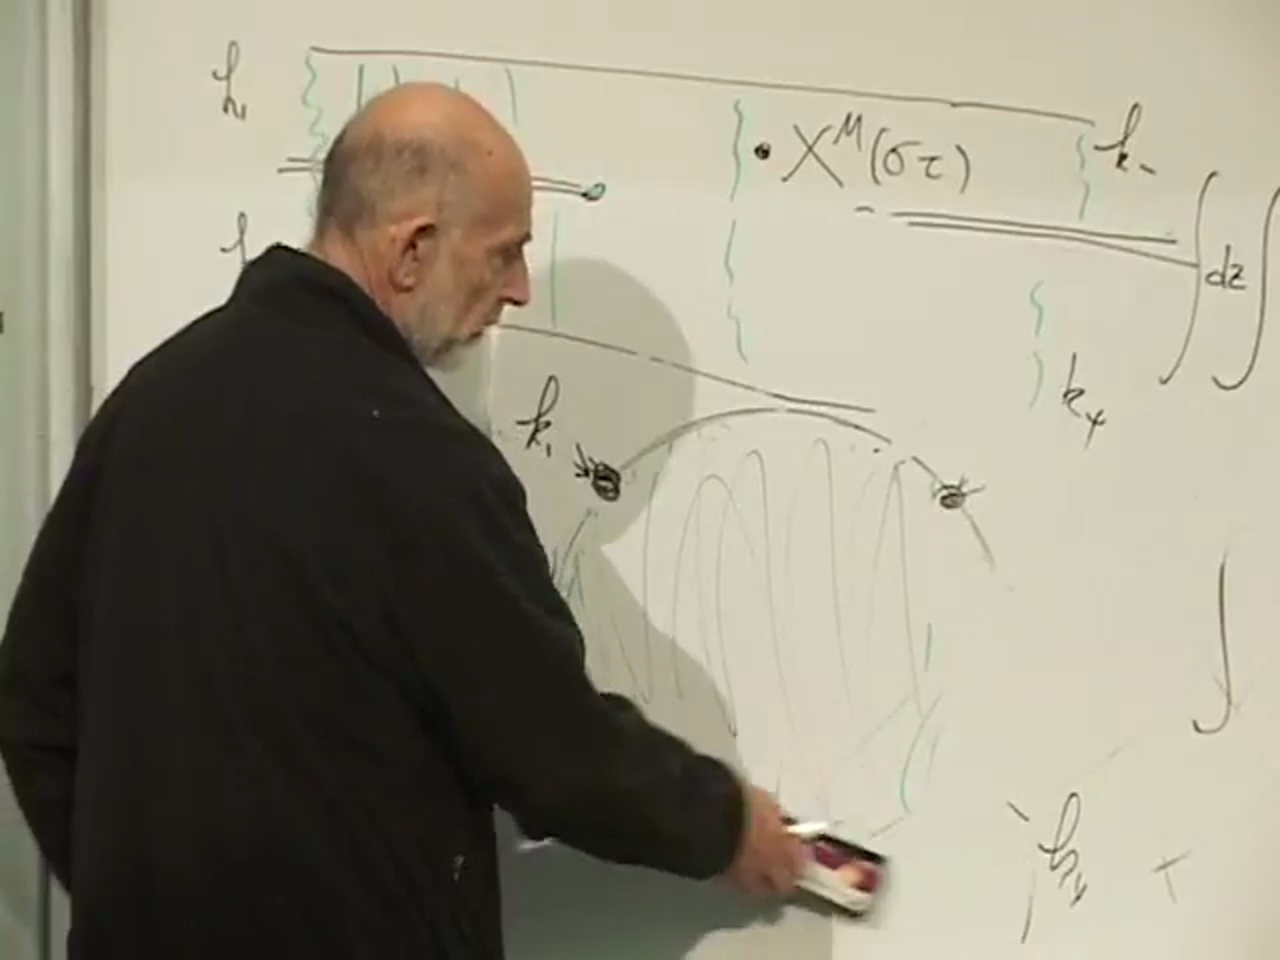
\includegraphics[width=0.72\textwidth]{lecture_08_figure_17.png}
  \caption{圆盘上的四个边界插入。共形自由度固定任意三个，留下一个四点模。}
  \lectureframe{01:35:18}
  \label{fig:l08-fix-three-board}
\end{figure}

\begin{classroomqa}
\audiencequestion{如果条带图中两个分裂点不在同一高度，会怎样？\lecturetimestamp{01:35:24}}
\lecturerresponse{共形映射可以把这种表观不匹配移走。不同的图是同一个模的不同坐标代表。不变的积分是对剩余边界位置的积分，等价地，也就是对传播间隔的积分。}
\end{classroomqa}

\begin{classroomqa}
\audiencequestion{对于更多的外部粒子，还剩下多少个位置参数？\lecturetimestamp{01:36:00}}
\lecturerresponse{利用共形对称性固定三个插入点，并对另外\(n-3\)个进行积分。这就是有序树级开弦振幅的边界模数计数。}
\end{classroomqa}

\begin{classroomqa}
\audiencequestion{这与M理论有何关系？\lecturetimestamp{01:36:37}}
\lecturerresponse{目前还没有。这里的构造是世界面上的微扰开弦散射。它与M理论的关系需要后来的对偶性和非微扰思想，因此这个问题被明确推迟。}
\end{classroomqa}

\begin{classroomqa}
\audiencequestion{不同的竖直或交叉条形图景是否是不同的计算？\lecturetimestamp{01:36:49}}
\lecturerresponse{不是。可以固定一个方便的点，并让其余的模数在其整个区间内变化。条形图景和圆盘上的边界点积分是同一个积分的不同切片方式，这就是为什么所有外部弦都可以被对称地处理。}
\end{classroomqa}

\section{该方案尚未解决的问题}

圆盘公式可以直接推广到更多外部弦：加入更多顶点算符，并对它们的\(n-3\)个不等价边界位置进行积分。对于一个自洽的弦模型来说，这是一个精确的树级方案，但它还不是一个关于已观测粒子物理的现实模型。简单的玻色子理论具有错误的时空维数和额外的物理缺陷。超弦改进了谱，并将临界维数降低到十，但仍然必须紧致化六个空间维度。

\begin{classroomqa}
\audiencequestion{这个简单模型是否已经与粒子碰撞实验一致？\lecturetimestamp{01:39:06}}
\lecturerresponse{不一致。其共振结构在历史上类似于强子散射，但二十六维玻色子模型不能直接描述已观测到的粒子。该形式体系为模型定义了散射振幅；要与自然相符，还需要现实的谱、紧致化、相互作用以及真空选择。}
\end{classroomqa}

\begin{classroomqa}
\audiencequestion{紧致化会减少额外维度并产生现实的粒子数据吗？\lecturetimestamp{01:41:10}}
\lecturerresponse{它可以降低有效宏观维度，并生成粒子谱和规范群。真正的数学困难也大多出现在这里。人们已经知道许多自洽的紧致化，但选择一个关于已观测基本粒子的唯一模型仍未解决。}
\end{classroomqa}

本讲强调这一区分，而不是宣传一个已经完成的理论。弦构造在数学上是确定的，并且已经产生了关于引力和几何的深刻信息，然而它们的多重性本身就是物理问题的一部分。

\begin{classroomqa}
\audiencequestion{有没有一种简短的方法来记住为什么玻色子临界维数是二十六？\lecturetimestamp{01:43:19}}
\lecturerresponse{先前的振子计算使用了正则化的零点求和\(1+2+3+\cdots=-1/12\)。横向振子贡献涉及二十四个方向，而恢复两个纵向时空坐标后得到\(24+2=26\)。这是对先前一致性论证的记忆法，而不是这里的新推导。}
\end{classroomqa}

\begin{classroomqa}
\audiencequestion{插入的动量\(k_i\)本身是量子化的吗？\lecturetimestamp{01:43:46}}
\lecturerresponse{在非紧致时空中，其分量是连续的。被量子化的是振子能级，从而是允许的质量平方谱。紧致维度可能会量子化相应的动量和绕数分量，但那属于下一次讨论。}
\end{classroomqa}

\chapter{弦、引力、紧致化与T对偶}

\lectureoverview{一个点粒子基本上可以在任何光滑几何上一致地运动，但量子弦不能。它无穷多的零点振荡依次探测越来越短的尺度上的靶空间，而当这些振荡被恢复时，有效几何会发生变化。要求这一过程具有不动点便给出\(R_{\mu\nu}=0\)，即真空爱因斯坦方程。随后我们从这一一致性条件转向紧致化。一个圆同时提供Kaluza--Klein动量态与弦缠绕态；交换它们便将半径为\(R\)的圆与半径为\(\alpha'/R\)的圆等同起来。}

\section{作为选择原理的一致性}

有两个问题需要回答。为什么引力会出现在弦理论中，以及为什么弦理论远比点粒子力学更不宽容？它们实际上是同一个问题。一个背景几何只有在一根弦能在其上传播而不保留对我们将弦分辨得多么精细的任意依赖时，才是可接受的。

从对照问题开始：一个被约束在光滑弯曲曲面上的点粒子。经典地，它沿测地线运动，即直线的内禀类比。人们可以用许多短线段来近似这一运动，写出差分方程，然后让线段长度趋于零。结果是一个具有良定义连续极限的常微分方程。

量子力学改变的是对历史的求和，而不是结论。我们不再选取一条经典路径，而是在曲面上的路径上对振幅求和。时间可以再次被分成小步，而该极限等价地由弯曲位形空间上的一个Schr\"odinger方程描述。对于光滑曲面，该极限稳定为一个确定的传播子和谱。

\begin{figure}[H]
  \centering
  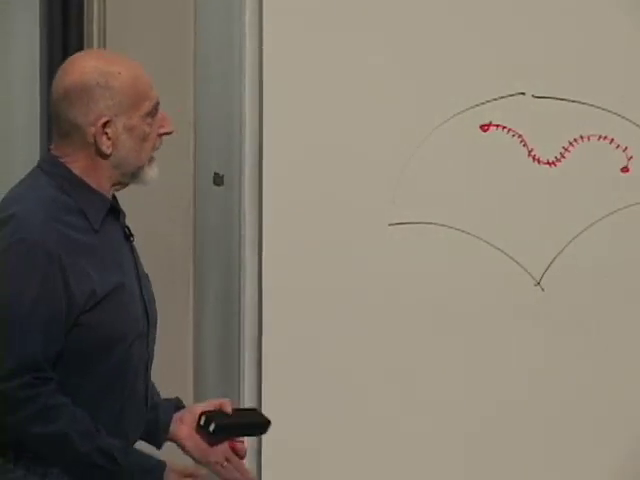
\includegraphics[width=0.72\textwidth]{lecture_09_figure_01.png}
  \caption{曲面上的光滑路径与来自时间切片量子求和的锯齿状路径。二者都保持为靶曲面的内禀对象。}
  \lectureframe{00:05:10}
  \label{fig:l09-particle-paths}
\end{figure}

\begin{classroomqa}
\audiencequestion{在路径积分中，是否要求所有路径都保持在曲面内部？\lecturetimestamp{00:05:39}}
\lecturerresponse{是的。曲面是粒子的位形空间，而不是嵌入在一个更大房间中的一张薄片，粒子不能穿过它走捷径。每一个中间点都属于该曲面，所有长度和作用量都用其内禀度规计算。}
\end{classroomqa}

对于弦，相应的问题更难。一根弦并不仅仅由质心位置来指定。它携带无穷多的振子塔，因此提高分辨率意味着允许更多的动力学自由度。只有当该塔被恢复时观测量趋于一个极限，理论才是一致的。

\section{球面上的点粒子}

球面是最简单的弯曲测试几何。设其半径为\(R\)，并首先将一个质量为\(m\)的粒子置于其上。对于沿大圆的运动，
\begin{equation}
  E=\frac{1}{2}mv^2=\frac{p^2}{2m},
  \qquad
  L=pR.
  \label{eq:l09-particle-energy}
\end{equation}
因此，
\begin{equation}
  E=\frac{L^2}{2mR^2}
   =\frac{L^2}{2I},
  \qquad
  I=mR^2.
  \label{eq:l09-rotor-energy}
\end{equation}
半径通过转动惯量进入。对角动量进行量子化便产生熟悉的刚性转子谱，而没有任何东西依赖于紫外截断。

\begin{figure}[H]
  \centering
  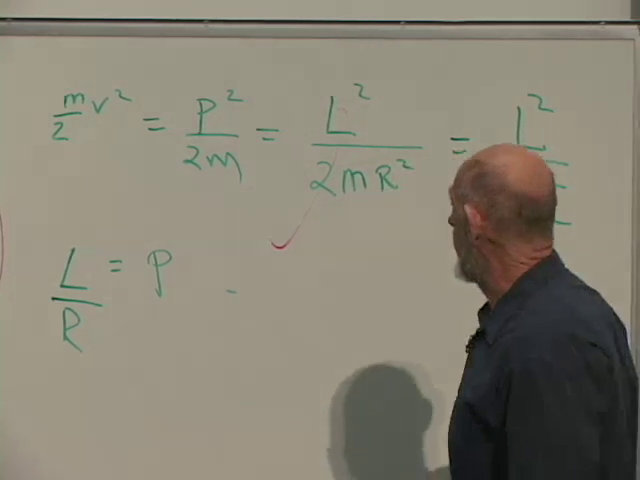
\includegraphics[width=0.74\textwidth]{lecture_09_figure_02.png}
  \caption{点粒子对照计算：
  \(p^2/(2m)=L^2/(2mR^2)=L^2/(2I)\)。}
  \lectureframe{00:11:25}
  \label{fig:l09-sphere-rotor}
\end{figure}

这个毫无困难的例子很重要。曲率本身并不是问题。当曲率与弦的内部量子延展耦合时，问题才出现。

\section{真空弦并非点状}

考虑开弦的一个横向坐标并减去其质心。这里所用的振子展开是示意性的：
\begin{equation}
  X(\sigma)-X_{\mathrm{cm}}
  \sim
  \sum_{n=1}^{\infty}
  \frac{a_n+a_n^\dagger}{\sqrt n}\cos(n\sigma).
  \label{eq:l09-mode-expansion}
\end{equation}
关键要素是余弦模、振子算符以及因子\(1/\sqrt n\)。精确归一化在尺寸论证中不起作用。
\editorialnote{精确展开包含依赖于约定的\(\alpha'\)因子、数值常数以及振子记号的选择。方程\eqref{eq:l09-mode-expansion}只保留了紫外估计所需的依赖关系，正如黑板推导中那样。}

\begin{figure}[H]
  \centering
  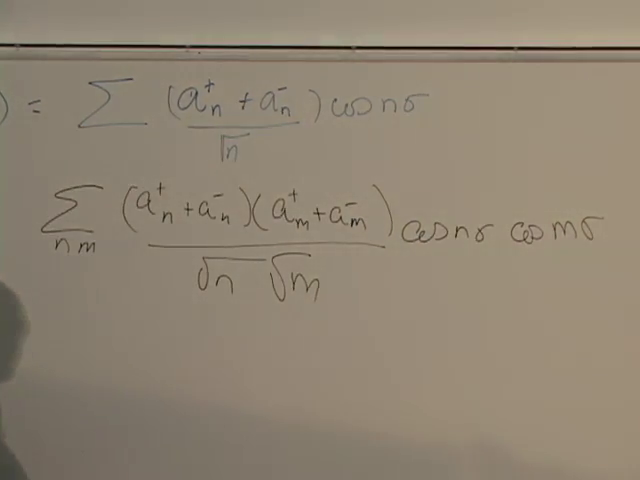
\includegraphics[width=0.78\textwidth]{lecture_09_figure_03.png}
  \caption{结构性的振子展开以及将其平方后得到的双重求和。}
  \lectureframe{00:15:20}
  \label{fig:l09-string-modes}
\end{figure}

在振子真空中，到质心的距离平方为
\begin{align}
  \expect{\bigl(X(\sigma)-X_{\mathrm{cm}}\bigr)^2}_0
  &\sim
  \sum_{n,m\geq1}
  \frac{\cos(n\sigma)\cos(m\sigma)}{\sqrt{nm}}\notag\\
  &\qquad\times
  \bra{0}(a_n+a_n^\dagger)\notag\\
  &\hspace{6em}\times(a_m+a_m^\dagger)\ket{0}.
  \label{eq:l09-size-double-sum}
\end{align}
大多数项都消失。两个湮灭算符将右矢消灭；两个产生算符留下一个与左矢正交的态；而一个产生算符后接一个湮灭算符在这种排序下也有零真空期望值。幸存的收缩为
\begin{equation}
  \bra{0}a_n a_m^\dagger\ket{0}=\delta_{nm}.
  \label{eq:l09-vacuum-contraction}
\end{equation}

\begin{figure}[H]
  \centering
  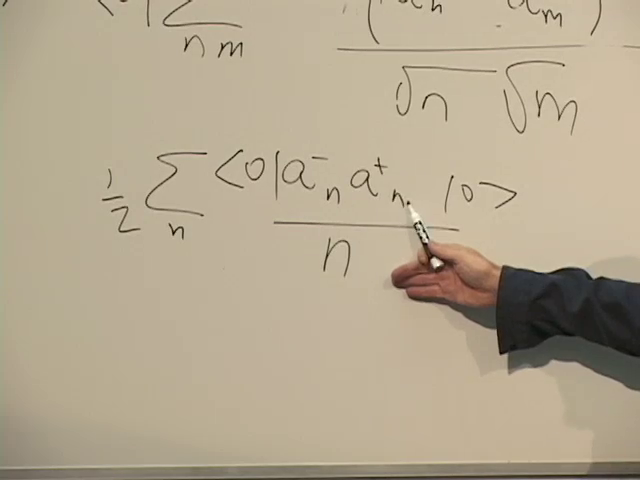
\includegraphics[width=0.74\textwidth]{lecture_09_figure_04.png}
  \caption{存活下来的真空收缩把双振子求和坍缩为单个求和。}
  \lectureframe{00:20:10}
  \label{fig:l09-vacuum-contraction}
\end{figure}

因此
\begin{equation}
  \expect{\bigl(X(\sigma)-X_{\mathrm{cm}}\bigr)^2}_0
  \sim
  \sum_{n=1}^{\infty}\frac{\cos^2(n\sigma)}{n}.
  \label{eq:l09-size-single-sum}
\end{equation}
在弦上的一个一般点处，或在对\(\sigma\)取平均之后，
\(\cos^2(n\sigma)\)大致贡献\(1/2\)。取模式截断
\(N\)，
\begin{equation}
  \expect{\bigl(X-X_{\mathrm{cm}}\bigr)^2}_{0,N}
  \sim
  \frac{1}{2}\sum_{n=1}^{N}\frac{1}{n}
  =\frac{1}{2}\log N+O(1).
  \label{eq:l09-logarithmic-size}
\end{equation}

\begin{figure}[H]
  \centering
  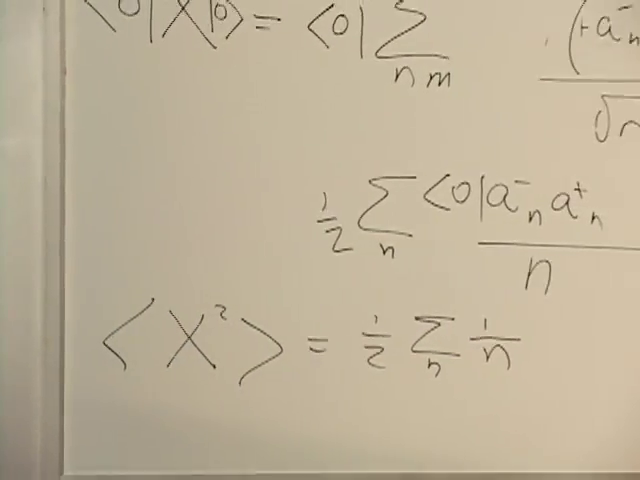
\includegraphics[width=0.72\textwidth]{lecture_09_figure_05.png}
  \caption{黑板上给出了控制基态展宽的调和求和。}
  \lectureframe{00:22:05}
  \label{fig:l09-harmonic-size}
\end{figure}

只保留比如说前二十五个模式，会得到一个有限的模糊客体，但它还不是连续弦。去掉截断会使均方展宽按对数增长。这一结论不应被误读为平直空间弦理论不自洽的证明。在平直空间中，质心运动与振子运动分离，物理振幅中精细的相消保持了预期的定域性。尺寸的增长是一个警告。曲率告诉我们这一警告是否会变成失败。

\section{当内部展宽改变几何时}

把弦放在球面的北极附近。当所有振子都被关闭时，它的行为就像刚才研究过的点粒子。随着更高模式被允许，弦变成一个在球冠上铺展开的涨落缠结。它的中心仍可绕球面运动，但进入转动能量的转动惯量所对应的客体现在是延展的。

对于穿过球心与两极的轴，
\begin{equation}
  I=\int r_\perp^2\,dm,
  \label{eq:l09-extended-inertia}
\end{equation}
其中\(r_\perp\)是弦元到该轴的垂直距离。轨道赤道处的一点具有最大的相关力臂。弦中向轴下垂的部分贡献较小。在总质量固定时，这降低了有效转动惯量：
\begin{equation}
  I_{\mathrm{eff}}<mR^2.
  \label{eq:l09-inertia-reduction}
\end{equation}
因此转动能量看起来像是一个位于更小球面上的点状客体的转动能量，
\begin{equation}
  E_{\mathrm{rot}}
  =\frac{L^2}{2I_{\mathrm{eff}}}
  \equiv \frac{L^2}{2mR_{\mathrm{eff}}^2},
  \qquad R_{\mathrm{eff}}<R.
  \label{eq:l09-effective-radius}
\end{equation}

\begin{classroomqa}
\audiencequestion{如果弦正在更大的区域上铺展开，为什么转动惯量会趋于零？\lecturetimestamp{00:33:23}}
\lecturerresponse{这一陈述是关于逐次粗粒化下的有效描述的，并不是说原始的延展分布立即具有零惯量。第一带模式把点变成一个模糊团块，其运动方式如同它生活在一个更小的球面上。下一带模式分辨出每个这样的团块内部的结构，并重复同样的重整化。迭代这一比较会把有效半径向内推。}
\end{classroomqa}

\begin{figure}[H]
  \centering
  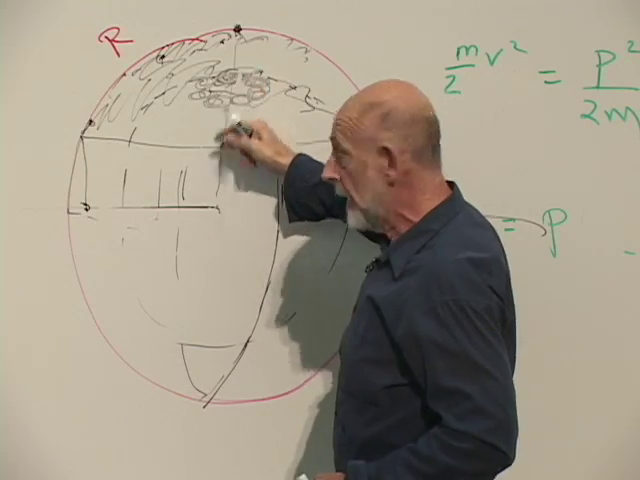
\includegraphics[width=0.72\textwidth]{lecture_09_figure_06.png}
  \medskip

  \begin{adjustbox}{max width=\linewidth}
  \begin{tikzpicture}[x=1cm,y=1cm,>=Latex]
    \draw[thick] (0,0) circle (2.15);
    \draw[dashed] (0,-2.55) -- (0,2.55);
    \draw[blue!65!black,thick]
      (-0.22,2.05)
      .. controls (-1.22,1.75) and (-1.52,1.08) .. (-1.06,0.44)
      .. controls (-0.55,-0.10) and (0.35,0.02) .. (1.10,0.68)
      .. controls (1.48,1.12) and (1.16,1.80) .. (0.20,2.05);
    \draw[red!70!black,dashed] (0,0) circle (1.25);
    \draw[->] (2.70,1.55) -- (4.05,1.55);
    \node[align=center] at (3.37,1.98) {add shorter\\modes};
    \draw[thick] (6.15,0) circle (1.25);
    \draw[dashed] (6.15,-1.65) -- (6.15,1.65);
    \draw[blue!65!black,thick]
      (6.00,1.18)
      .. controls (5.42,0.88) and (5.46,0.25) .. (6.02,-0.06)
      .. controls (6.46,-0.28) and (6.90,0.45) .. (6.28,1.18);
    \node at (0,-3.00) {sphere of radius \(R\)};
    \node at (6.15,-2.05) {effective radius \(R_{\mathrm{eff}}\)};
  \end{tikzpicture}
  \end{adjustbox}
  \caption{黑板上的北极弦以及有效半径论证的清晰重构。虚线内圆是一种有效几何，而不是球面内部的第二个物理壳层。}
  \lectureframe{00:35:15}
  \label{fig:l09-shrinking-sphere}
\end{figure}

这是一个重整化群陈述。有限截断使弦成为一个具有有限内部分辨率的团块。提高截断会改变该团块的力学。在正曲率球面上，每增加一层模式壳都会使从长距离运动推断出的背景变小。如果结果永不稳定，那么在该背景上就不存在与截断无关的弦理论。

\section{度规必须达到不动点}

现在把球面替换为一般的目标空间度规
\(g_{\mu\nu}(x)\)。在振子模式的薄对数壳层中积分会以局部对称二阶张量的形式改变该度规。这一改变必须在平直空间中消失，并且从度规的两个导数开始。在领头阶，协变性使里奇张量成为相关候选：
\begin{equation}
  \frac{\partial g_{\mu\nu}}{\partial\log\Lambda}
  =-C\,R_{\mu\nu}+\cdots ,
  \qquad C>0
  \label{eq:l09-ricci-flow}
\end{equation}
其方向对应于几何论证中所用的粗粒化方向。于是正曲率会把球面向内驱动，正如所需。
\editorialnote{归一化和符号取决于重整化参数是朝紫外还是朝红外增加。在通常的世界面记号中，领头度规贝塔函数是\(\beta^g_{\mu\nu}=\alpha'R_{\mu\nu}+\cdots\)。这里所用的不变量陈述是：截断无关性要求贝塔函数，因而在此阶要求\(R_{\mu\nu}\)，为零。}

\begin{figure}[H]
  \centering
  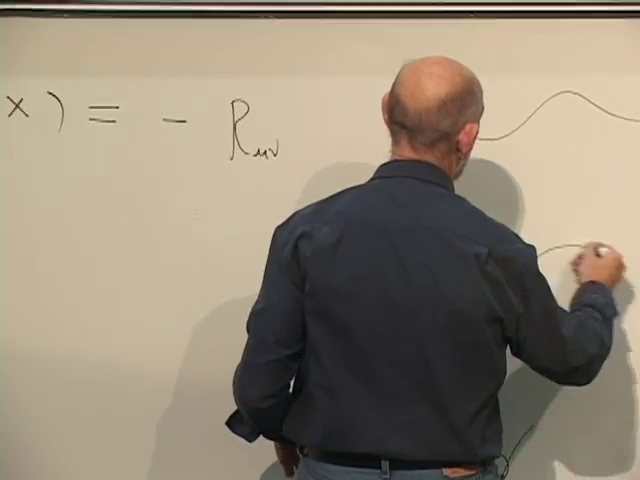
\includegraphics[width=0.76\textwidth]{lecture_09_figure_07.png}
  \caption{度规改变被示意性地写成负的里奇张量，旁边画有一条平滑曲线。}
  \lectureframe{00:43:00}
  \label{fig:l09-ricci-flow-board}
\end{figure}

\begin{classroomqa}
\audiencequestion{振子截断\(N\)在这个流方程中出现在哪里？\lecturetimestamp{00:43:38}}
\lecturerresponse{它就是标度变量。当所包含的最高模发生变化时，弦尺度求和按对数方式改变，因此自然的演化参数是\(\log N\)，或者等价地是\(\log\Lambda\)。方程\eqref{eq:l09-ricci-flow}描述了一个对数壳层模式所引起的无穷小变化。}
\end{classroomqa}

可容许的背景是这个流的不动点。在领头阶，
\begin{equation}
  \boxed{R_{\mu\nu}=0.}
  \label{eq:l09-ricci-flat}
\end{equation}
Ricci 平坦并不意味着 Riemann 张量的每一个分量都为零。例如，引力波在真空中可以具有非零曲率，同时满足\(R_{\mu\nu}=0\)。

\subsection{同一条件就是真空 Einstein 方程}

在抑制掉常规常数后，Einstein 方程为
\begin{equation}
  G_{\mu\nu}
  \equiv
  R_{\mu\nu}-\frac12 g_{\mu\nu}R
  =T_{\mu\nu}.
  \label{eq:l09-einstein}
\end{equation}

\begin{figure}[H]
  \centering
  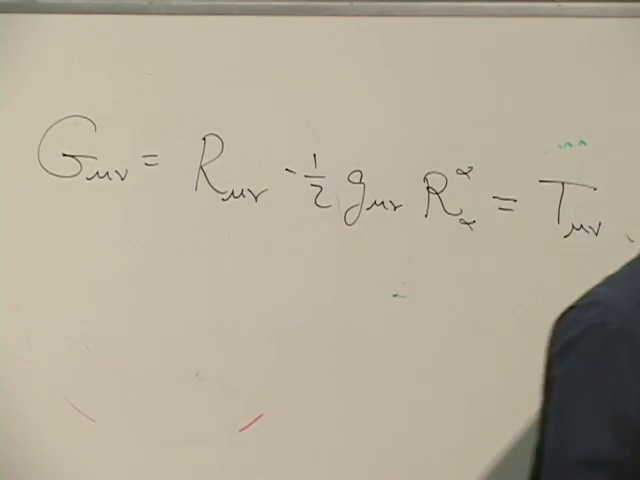
\includegraphics[width=0.78\textwidth]{lecture_09_figure_08.png}
  \caption{黑板上的 Einstein 张量与应力张量。}
  \lectureframe{00:47:15}
  \label{fig:l09-einstein-board}
\end{figure}

在真空中\(T_{\mu\nu}=0\)。在\(D\)维时空中取迹得到
\begin{equation}
  0=g^{\mu\nu}G_{\mu\nu}
   =\left(1-\frac{D}{2}\right)R.
  \label{eq:l09-einstein-trace}
\end{equation}
对于\(D\neq2\)，有\(R=0\)，再代回\eqref{eq:l09-einstein}便得到\(R_{\mu\nu}=0\)。因此，弦失去其对截断的依赖这一条件就是真空引力场方程。引力并不是被附加到理论上的；它是作为一致性的代价而出现的。

\emph{真空}一词并不意味着什么都不发生。它意味着该区域内没有应力-能量源。无源的 Maxwell 方程允许电磁波，无源的 Einstein 方程允许引力波。即使其 Ricci 张量为零，几何仍然可以是动力学的。

\begin{classroomqa}
\audiencequestion{这个条件与共形不变性有关吗？\lecturetimestamp{00:52:20}}
\lecturerresponse{是的，尽管这个问题在录音中有一部分丢失了。相关的对称性是\emph{世界面}量子理论的共形不变性。要求世界面标度反常消失，正是使度规 beta 函数为零的条件。不应把它与要求时空本身共形不变混淆起来。}
\end{classroomqa}

还有第二个一致性条件。世界面共形不变性还确定了临界时空维度：超弦为十维，玻色弦为二十六维。因此，仅 Ricci 平坦并不是全部要求，但它是最直接地显示出 Einstein 方程的那一部分。

\section{紧致维度而非缺失维度}

超弦背景有九个空间维度和一个时间维度。我们的宏观世界只显示出三个大的空间方向，因此六个空间维度必须在通常尺度下被隐藏起来，或者以其他方式变得不可及。紧致化使它们保持为真正的维度，同时赋予它们小的有限尺度。

\begin{classroomqa}
\audiencequestion{如果不同的观测者携带不同的时钟，那是否相当于拥有不止一个时间维度？\lecturetimestamp{00:56:59}}
\lecturerresponse{不。许多时钟只是许多测量一个时空中坐标的仪器；它们并不会创造出独立的类时方向。这里考虑的额外维度是空间性的。熟悉的量子构造和因果构造并不能提供一种可与之相比的、具有多个局部时间方向的一致理论，因此那种可能性不属于这个紧致化模型。}
\end{classroomqa}

想象一些生物，它们相信自己的世界是一条线。在低分辨率下，它们只能向前和向后移动。然而，在足够强大的显微镜下，这条线被揭示为一个非常细的圆柱。一个小生物除了可以沿着它的长度移动外，还可以绕着它的圆周方向移动。第二个方向一直存在；只是它的周长太小，粗糙的探测无法分辨。

\begin{figure}[H]
  \centering
  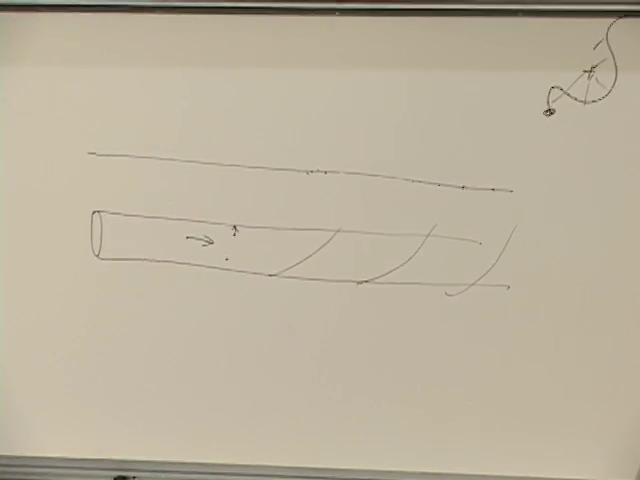
\includegraphics[width=0.78\textwidth]{lecture_09_figure_09.png}
  \caption{一个狭窄的圆柱以及绕其隐藏圆周方向缠绕的轨迹。}
  \lectureframe{01:01:00}
  \label{fig:l09-hidden-cylinder}
\end{figure}

圆柱可以表示为一个带，其上边缘和下边缘被等同起来。穿过上边缘会从下边缘的同一纵向位置返回。两个边缘处都没有物理边界。同样的操作可以用两个方向来进行：把一个矩形的左边缘和右边缘等同起来，同时也把它的上边缘和下边缘等同起来。结果就是一个二维环面。

\begin{figure}[H]
  \centering
  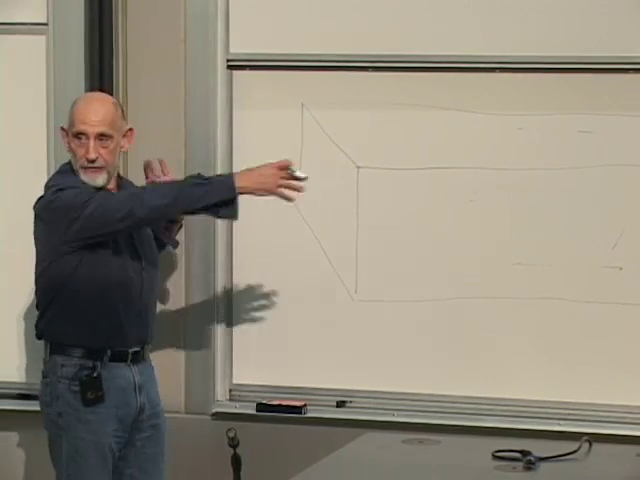
\includegraphics[width=0.76\textwidth]{lecture_09_figure_10.png}
  \medskip

  \begin{tikzpicture}[x=0.82cm,y=0.82cm,>=Latex]
    \draw[thick] (0,0) rectangle (4,2.15);
    \draw[blue!65!black,->] (0,2.48) -- (4,2.48);
    \draw[blue!65!black,->] (4,-0.34) -- (0,-0.34);
    \node at (2,-0.82) {one periodic direction};
    \draw[thick] (6.1,0) rectangle (10.1,2.15);
    \draw[blue!65!black,->] (6.1,2.48) -- (10.1,2.48);
    \draw[blue!65!black,->] (10.1,-0.34) -- (6.1,-0.34);
    \draw[red!70!black,->] (5.76,0) -- (5.76,2.15);
    \draw[red!70!black,->] (10.44,2.15) -- (10.44,0);
    \node at (8.1,-0.82) {two periodic directions};
  \end{tikzpicture}
  \caption{黑板上的板条以及一个干净的基本区域描述。等同一对边缘得到圆柱；等同两对边缘得到环面。}
  \lectureframe{01:04:40}
  \label{fig:l09-periodic-identification}
\end{figure}

环面首先是一种拓扑，其次才是三维空间中形如面包圈的曲面。把环面剪一刀，它就变成一个圆柱面；再剪一刀，它就变成一个矩形，前提是记住边的粘合方式。可以在这个矩形上放置一个平坦度规，因此所得的平坦环面局部具有零黎曼曲率，当然也是里奇平坦的。

矩形上的一条直线轨迹穿过一条被粘合的边后仍保持直线。如果它的斜率是两个周期的有理比，轨迹最终会闭合。如果这个比是无理数，它就永不闭合，并会在环面上变得稠密。

\begin{figure}[H]
  \centering
  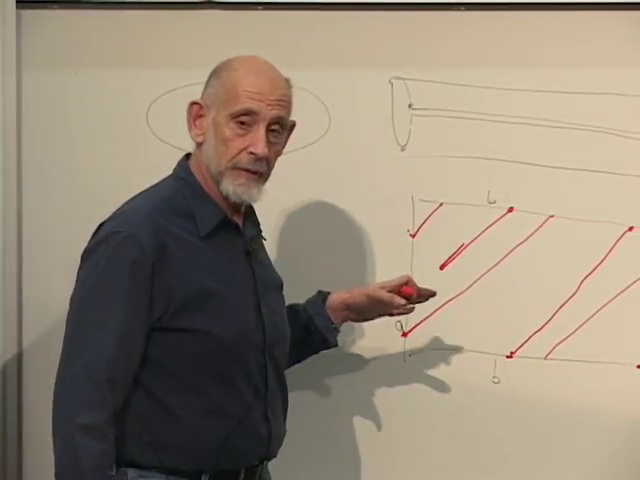
\includegraphics[width=0.76\textwidth]{lecture_09_figure_11.png}
  \caption{基本域中反复出现的直线段代表环面上的一条不间断轨迹。}
  \lectureframe{01:11:00}
  \label{fig:l09-torus-trajectory}
\end{figure}

高维环面以同样的方式构成。把立方体的每一对相对面粘合起来就得到一个三环面，而六个紧致方向可以用一个六环面来建模。不应试图把所有这些对象都嵌入普通的三维空间；面粘合的描述是内蕴的，也是完备的。

\begin{classroomqa}
\audiencequestion{额外维度是否必然要卷回到自身？
\lecturetimestamp{01:15:03}}
\lecturerresponse{并非作为一条定理。它也可以是非紧致的，但那样它通常会作为观测到的长距离世界中的另一个大方向而出现。紧致性是使额外维度与其表面上的缺失相协调的最简单方式。自然界为何选择某种特定的紧致化，则是一个独立的动力学问题。}
\end{classroomqa}

\begin{classroomqa}
\audiencequestion{为什么要假设那些看不见的维度是以这种方式卷曲起来的普通空间方向，而不是某种完全不同的东西？\lecturetimestamp{01:15:51}}
\lecturerresponse{因为这是一个确定的、可求解的假设，而不是因为它已被证明是对自然界的唯一描述。紧致空间流形使我们能够构造自洽的例子并计算其谱。更奇异的可能性必须通过做到同样的事情来赢得自己的位置。}
\end{classroomqa}

\begin{classroomqa}
\audiencequestion{熟悉的面包圈形环面上的距离看起来并不像矩形中的距离。这里指的是哪一种几何？
\lecturetimestamp{01:18:11}}
\lecturerresponse{\emph{环面}一词固定的是粘合方式，而不是某一个唯一的度规。嵌入的面包圈从三维空间继承了一个弯曲度规。周期粘合的矩形则带有一个平坦度规。它们具有相同的拓扑和不同的几何；对于这里所说的简单紧致化，我们指的是平坦的那一个。}
\end{classroomqa}

\section{平坦环面的形状参数}

即便是一个平坦的二环面也不是唯一的。它的基本平行四边形有一个总面积、一个长宽比和一个剪切。改变这些参数会改变距离，从而改变谱，但不改变拓扑。

\begin{figure}[H]
  \centering
  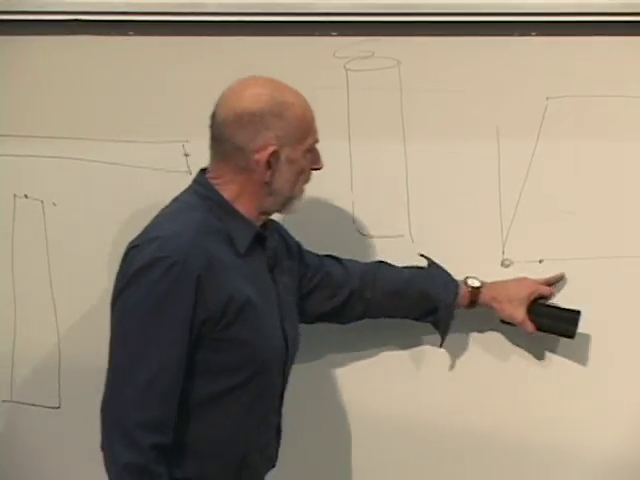
\includegraphics[width=0.74\textwidth]{lecture_09_figure_12.png}
  \medskip

  \begin{tikzpicture}[x=0.9cm,y=0.9cm,>=Latex]
    \draw[thick] (0,0) rectangle (3.4,2.1);
    \draw[<->] (0,-0.35) -- node[below] {\(L_1\)} (3.4,-0.35);
    \draw[<->] (-0.35,0) -- node[left] {\(L_2\)} (-0.35,2.1);
    \draw[thick] (5.4,0) -- (8.8,0) -- (9.7,2.1) -- (6.3,2.1) -- cycle;
    \draw[dashed] (5.4,0) -- (6.3,2.1);
    \draw[->] (5.75,2.48) -- node[above] {shear} (6.45,2.48);
    \node at (1.7,-1.00) {area and aspect ratio};
    \node at (7.55,-1.00) {complex structure};
  \end{tikzpicture}
  \caption{用于讨论环面模数的矩形基本域和剪切基本域。}
  \lectureframe{01:23:00}
  \label{fig:l09-torus-moduli}
\end{figure}

对于二环面，把形状打包成一个复数\(\tau=\tau_1+i\tau_2\)是有用的：实部记录剪切，虚部在分离出整体标度后记录长宽比。交换两个基本循环或改变它们的整数基，可以使表面上不同的平行四边形描述同一个环面。

\begin{classroomqa}
\audiencequestion{如果在粘合之前把一条边翻转，会发生什么？\lecturetimestamp{01:24:20}}
\lecturerresponse{那会产生一种不同的拓扑。用反射来粘合会得到一个不可定向曲面，即克莱因瓶，而不是普通的环面。}
\end{classroomqa}

\begin{classroomqa}
\audiencequestion{如果扭转沿边不是均匀的呢？
\lecturetimestamp{01:25:01}}
\lecturerresponse{一个光滑的非均匀形变可以被转移到基本域上的度规中。拓扑粘合与几何数据必须保持区分：改变粘合方式可能改变拓扑，而光滑地改变距离则改变度规。}
\end{classroomqa}

\editorialnote{对于平坦二环面，面积是最简单的凯勒模数，而\(\tau\)是复结构模数。连续的剪切是\(\tau\)的一部分。德恩扭转则是一种离散的映射类操作，由\(\tau\mapsto\tau+1\)表示；它本身并不是那个连续模数。这澄清了黑板讨论中所使用的有意非正式的术语。}

平坦环面之所以有用，是因为它们立即满足自洽性条件，但它们的对称性对于粒子物理的现实模型来说过于宽裕。更精细的里奇平坦空间，尤其是卡拉比--丘流形，提供了更丰富的紧致化。它们的详细构造超出了本讨论的范围；原理仍然相同。

\section{从谱中读出紧致圆}

休息之后，把紧致空间约化为一个周长为
\(2\pi R\)的圆。波函数绕行一周后必须单值：
\begin{equation}
  e^{ip_c(x+2\pi R)/\hbar}=e^{ip_cx/\hbar}.
\end{equation}
因此
\begin{equation}
  p_cR=n\hbar,
  \qquad
  p_c=\frac{n\hbar}{R},
  \qquad n\in\mathbb Z.
  \label{eq:l09-kk-momentum}
\end{equation}

\begin{figure}[H]
  \centering
  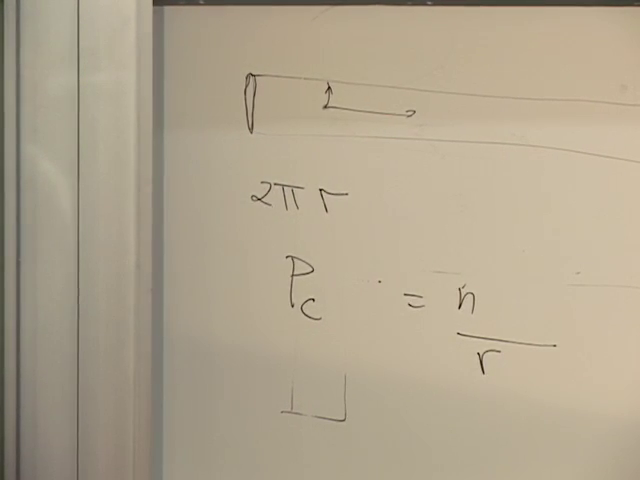
\includegraphics[width=0.74\textwidth]{lecture_09_figure_13.png}
  \caption{紧致周长\(2\pi R\)与量子化动量
  \(p_c=n\hbar/R\)。}
  \lectureframe{01:32:15}
  \label{fig:l09-kk-board}
\end{figure}

对于全时空中的无质量粒子，
\begin{equation}
  E=c|\mathbf P|.
  \label{eq:l09-massless-dispersion}
\end{equation}

\begin{figure}[H]
  \centering
  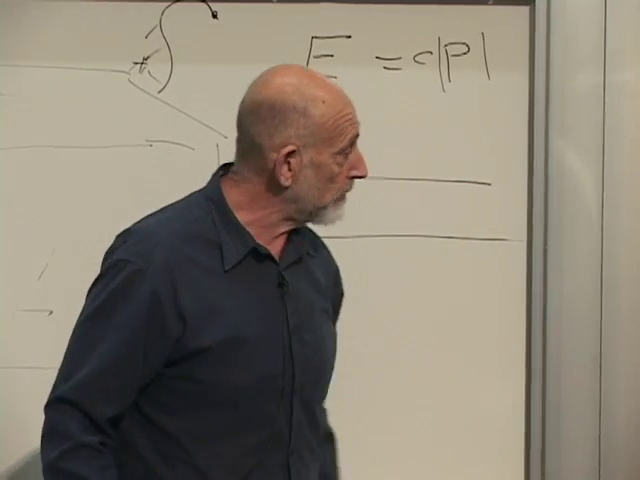
\includegraphics[width=0.70\textwidth]{lecture_09_figure_14.png}
  \caption{用于把紧致动量重新解释为低维质量的无质量色散关系。}
  \lectureframe{01:33:45}
  \label{fig:l09-massless-board}
\end{figure}

把动量分成非紧致部分与紧致部分，并令
\(c=\hbar=1\)：
\begin{equation}
  E^2=\mathbf p_{\mathrm{large}}^2+\frac{n^2}{R^2}.
  \label{eq:l09-kk-dispersion}
\end{equation}
无法分辨紧致方向的观测者将它与
\(E^2=\mathbf p_{\mathrm{large}}^2+m^2\)相比较，推断出一系列质量
\begin{equation}
  m_n=\frac{|n|}{R}.
  \label{eq:l09-kk-masses}
\end{equation}
\(n\)的两个符号描述的是具有相同正能量的相反紧致动量，而不是正质量和负质量。因此，间距\(1/R\)通过光谱揭示了半径。这就是
Kaluza--Klein机制：隐藏方向上的动量在可见维度中表现为质量。

\section{缠绕态补全谱}

闭弦具有一种点粒子不具备的可能性：它可以缠绕在圆上。若缠绕数为\(w\)，则弦只有在绕紧致方向\(w\)圈后才闭合。其长度为
\(2\pi |w|R\)，因此张力提供能量
\begin{equation}
  m_w
  =2\pi T\,|w|R
  =\frac{|w|R}{\alpha'}.
  \label{eq:l09-winding-mass}
\end{equation}
本讲选取\(\alpha'=1\)的单位，将其约化为
\begin{equation}
  m_w=|w|R.
  \label{eq:l09-winding-lecture-units}
\end{equation}
正的和负的\(w\)是绕圆的相反取向。

\begin{figure}[H]
  \centering
  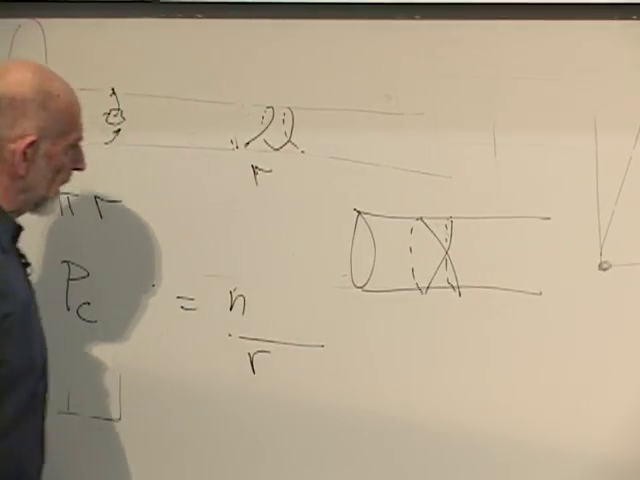
\includegraphics[width=0.76\textwidth]{lecture_09_figure_15.png}
  \caption{缠绕在紧致圆柱上的闭弦，黑板上标出了紧致半径。}
  \lectureframe{01:39:45}
  \label{fig:l09-winding-board}
\end{figure}

因此，紧致圆产生两个互补的阶梯：
\begin{equation}
  m_n=\frac{|n|}{R},
  \qquad
  m_w=\frac{|w|R}{\alpha'}.
  \label{eq:l09-two-towers}
\end{equation}
当\(R\)大时，动量能级间距小，而缠绕态很重。当\(R\)小时，动量能级间距大，而缠绕态很轻。

\begin{figure}[H]
  \centering
  \begin{tikzpicture}[x=1cm,y=0.9cm,>=Latex]
    \draw[->] (0,0) -- (0,4.7) node[above] {\(m\)};
    \foreach \y/\lab in {0/0,1.1/{1/R},2.2/{2/R},3.3/{3/R},4.4/{4/R}} {
      \draw (-0.16,\y) -- (0.16,\y);
      \node[left] at (-0.22,\y) {\(\lab\)};
    }
    \node at (0,-0.62) {momentum};
    \draw[<->,very thick,blue!65!black] (2.05,2.15) -- (4.05,2.15)
      node[midway,above] {\(R\leftrightarrow\alpha'/R\)};
    \draw[->] (6.1,0) -- (6.1,4.7) node[above] {\(m\)};
    \foreach \y/\lab in {0/0,1.1/{R/\alpha'},2.2/{2R/\alpha'},3.3/{3R/\alpha'},4.4/{4R/\alpha'}} {
      \draw (5.94,\y) -- (6.26,\y);
      \node[right] at (6.32,\y) {\(\lab\)};
    }
    \node at (6.1,-0.62) {winding};
  \end{tikzpicture}
  \caption{当半径以弦单位取倒数时，动量阶梯与缠绕阶梯互换。}
  \label{fig:l09-dual-mass-towers}
\end{figure}

\section{T对偶：小圆与大圆是相同的物理}

两个阶梯通过
\begin{equation}
  R\longleftrightarrow\frac{\alpha'}{R},
  \qquad
  n\longleftrightarrow w.
  \label{eq:l09-t-duality}
\end{equation}互换。
在黑板上所用的单位中，\(\alpha'=1\)，因此这简单地就是
\(R\leftrightarrow1/R\)。在自对偶半径
\(R=\sqrt{\alpha'}\)处，动量标度与缠绕标度重合。

\begin{figure}[H]
  \centering
  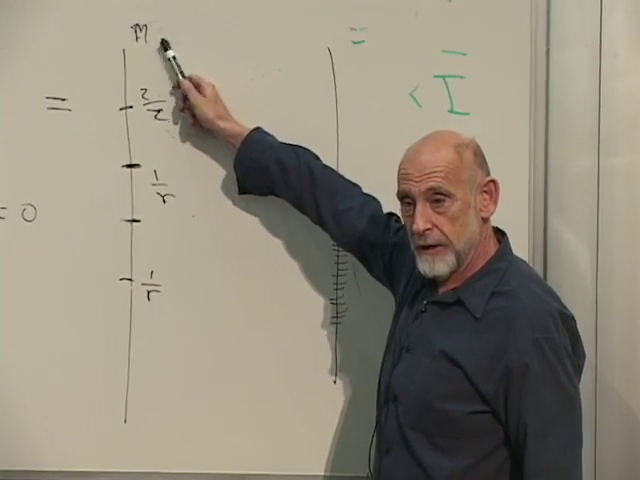
\includegraphics[width=0.74\textwidth]{lecture_09_figure_16.png}
  \caption{黑板上比较了半径越过自对偶标度时稀疏与稠密的质量阶梯。}
  \lectureframe{01:43:00}
  \label{fig:l09-duality-board}
\end{figure}

基本质量公式的互换只是这一结果可见的边缘。闭弦振子态与散射振幅也被一致地映射。比弦标度更小的圆并不是一种新的、越来越小的几何；它有一个作为更大对偶圆的等价描述。点粒子无法作出这种等同，因为它们拥有动量模但没有缠绕模。

\begin{classroomqa}
\audiencequestion{这难道仅仅等同于交换一个竖直方向和一个水平方向吗？\lecturetimestamp{01:44:38}}
\lecturerresponse{不。它交换的是两个不同的量子数：绕圆的动量与闭弦缠绕圆的次数。半径必须同时取倒数。}
\end{classroomqa}

\begin{classroomqa}
\audiencequestion{在\(R<\sqrt{\alpha'}\)和
\(R>\sqrt{\alpha'}\)处的描述只涉及玻色子，还是也涉及费米子？
\lecturetimestamp{01:46:30}}
\lecturerresponse{这种对偶性是整个紧致化弦理论的对称性，而不只是用来揭示它的简单玻色子质量阶梯的对称性。各扇区的详细映射取决于理论，但小--大的等价性并不限于一种粒子。}
\end{classroomqa}

\begin{classroomqa}
\audiencequestion{所比较的两个态是开弦还是闭弦？\lecturetimestamp{01:47:32}}
\lecturerresponse{它们是闭弦态。自由传播的闭弦可以缠绕紧致圆。端点自由的普通开弦不携带同样的守恒缠绕数。}
\end{classroomqa}
\editorialnote{在更完整的开弦论述中，T对偶交换Neumann边界条件与Dirichlet边界条件，并引入D膜。这就是为什么开弦的T对偶比简单照搬闭弦缠绕公式更为丰富。}

\begin{classroomqa}
\audiencequestion{这种互换是否类似于黑洞视界附近空间与时间的交换？\lecturetimestamp{01:48:00}}
\lecturerresponse{不是。视界坐标与因果性质是另一个不同的问题。这里两种描述涉及的是同一个紧致空间圆以及其动量扇区与缠绕扇区的交换。}
\end{classroomqa}

\begin{classroomqa}
\audiencequestion{这是否通过给出一个最小长度而解决了短距离自能问题？\lecturetimestamp{01:48:35}}
\lecturerresponse{它表明，小于弦尺度的半径并不定义新的不等价的圆背景：将\(R\)减小到自对偶点以下会增大对偶半径。这是对探测任意小圆几何的一种精确的弦论障碍，尽管不应把它变成这样一种主张：每一个可以想象的距离概念都有一个普适的硬性下界。}
\end{classroomqa}

\section{为什么缠绕扇区不能被省略}

\begin{classroomqa}
\audiencequestion{我们能否只用未缠绕的弦来定义理论，而把缠绕态排除在外？\lecturetimestamp{01:48:56}}
\lecturerresponse{不能。闭弦相互作用会产生它们。把一个未缠绕的圈沿紧致方向拉伸，使得一段沿一个方向绕圆，另一段沿相反方向绕圆。净缠绕仍然为零。随后一次重联可以把该圈分裂成两个闭弦，其缠绕数分别为\(+1\)和\(-1\)。这一对可以分开，因此即使初始态没有缠绕态，缠绕态也必须属于谱。}
\end{classroomqa}

\begin{figure}[H]
  \centering
  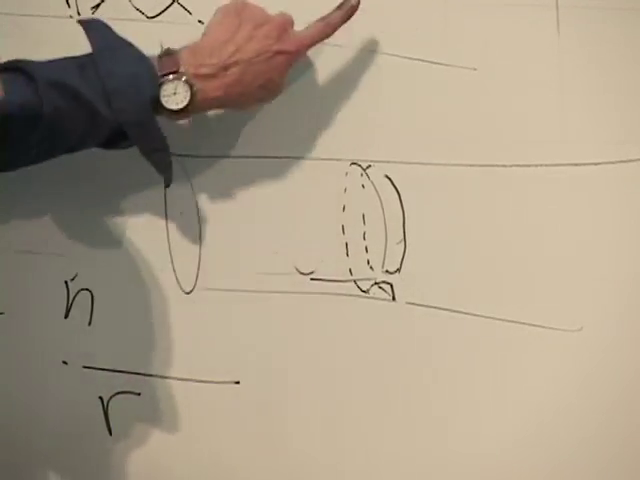
\includegraphics[width=0.74\textwidth]{lecture_09_figure_17.png}
  \caption{重联前围绕紧致方向排列的拉伸的零缠绕圈。}
  \lectureframe{01:50:30}
  \label{fig:l09-winding-pair-before}
\end{figure}

\begin{figure}[H]
  \centering
  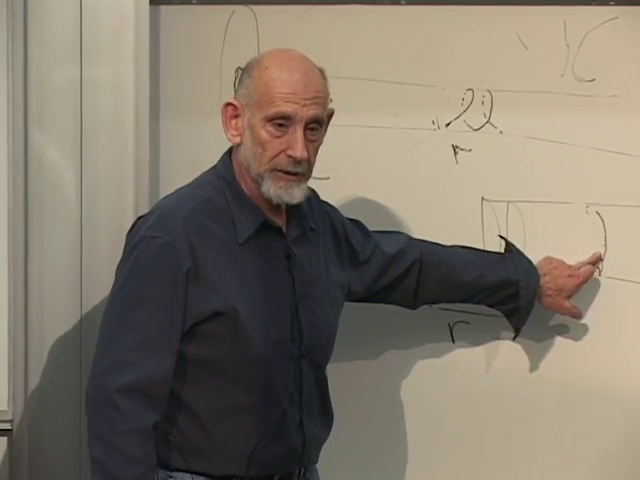
\includegraphics[width=0.72\textwidth]{lecture_09_figure_18.png}
  \medskip

  \begin{tikzpicture}[x=0.9cm,y=0.9cm,>=Latex]
    \draw[thick] (0,0) ellipse (1.0 and 1.55);
    \draw[blue!65!black,thick]
      (0.08,1.35) .. controls (2.0,1.15) and (2.0,-1.15) .. (0.08,-1.35);
    \draw[red!70!black,thick]
      (-0.08,-1.35) .. controls (-2.0,-1.15) and (-2.0,1.15) .. (-0.08,1.35);
    \node at (0,-2.15) {net \(w=0\)};
    \draw[->,thick] (2.45,0) -- (3.75,0) node[midway,above] {split};
    \draw[thick] (5.05,0.62) ellipse (0.68 and 1.02);
    \draw[blue!65!black,very thick,->]
      (5.05,1.64) arc[start angle=90,end angle=-250,x radius=0.68,y radius=1.02];
    \node at (5.05,-0.82) {\(w=+1\)};
    \draw[thick] (7.45,0.62) ellipse (0.68 and 1.02);
    \draw[red!70!black,very thick,<-]
      (7.45,1.64) arc[start angle=90,end angle=-250,x radius=0.68,y radius=1.02];
    \node at (7.45,-0.82) {\(w=-1\)};
  \end{tikzpicture}
  \caption{黑板上分开的缠绕圈以及缠绕--反缠绕对产生的清晰重构。总缠绕保持为零。}
  \lectureframe{01:51:30}
  \label{fig:l09-winding-pair-after}
\end{figure}

\begin{classroomqa}
\audiencequestion{产生缠绕对是否需要额外能量？\lecturetimestamp{01:52:11}}
\lecturerresponse{需要。拉伸一根弦要付出张力能量，而最终缠绕的弦具有\eqref{eq:l09-winding-mass}中的质量。一次能量足够高的碰撞可以产生这一对，正如一次碰撞可以产生一个粒子及其反粒子，同时保持相关的守恒荷。}
\end{classroomqa}

\section{人能听出弦背景的形状吗？}

对于普通的紧致化粒子理论，Kaluza--Klein谱的间距让我们推断半径：人们试图从其简正模听出紧致空间的形状。弦理论使这个逆问题变得更加微妙。动量模听到\(1/R\)，缠绕模听到\(R/\alpha'\)，而当两者互换时，完整谱保持不变。点粒子几何视为不同的两个半径，其实是用对偶变量描述的同一个弦背景。

因此，本讲通过一条途径得出了它所承诺的两个结论。紫外一致性迫使靶空间度规满足真空爱因斯坦方程，所以引力不可避免。紧致化随后把隐藏的几何变成粒子谱，但缠绕态阻止该谱在弦尺度以下指定一个唯一的经典半径。一致性不仅仅选择哪些几何是允许的；通过T对偶，它改变了什么才算作不同的几何。

\chapter{T对偶、D膜与规范理论}

\lectureoverview{T对偶最初表现为半径为(R)的圆上的闭弦与\(\alpha'/R\)上的闭弦之间的精确等价。动量与缠绕互换角色，世界面导数\(\partial_\tau Y\)与\(\partial_\sigma Y\)也互换角色，由\(G_{\mu 5}\)与\(B_{\mu 5}\)导出的时空矢量同样互换。当把同样的操作施加于开弦时，Neumann端点条件变为Dirichlet条件。端点因此必须位于一个动力学D膜上。被限制在一张膜上的开弦在低能下产生阿贝尔规范理论；连接一叠膜的弦带有两个端点标记，产生非阿贝尔规范理论。终止于D3膜上的D弦提供相应的磁单极子。}

\section{为什么要回到T对偶？}

我们已经遇到过T对偶，但回到它是有理由的。它是表明弦理论所包含的内容远多于微扰弦的线索之一。一旦理解了它对开弦的后果，它就引出了D膜；D膜反过来又成为构造和研究量子场论的一种方式。因此，本讲的目的不仅仅是重复“小圆等价于大圆”这一口号。我们将足够仔细地重建论证，以看清这一口号如何把新的物理对象强加进理论之中。

最简单的设定是环面紧致化。一维环面就是一个圆。二维环面可以用一个对边等同的平行四边形来表示，三维环面则可以用一个对面等同的平行六面体来表示。同样的构造可以继续到更高维。我们将只保留一个紧致空间坐标，称为\(Y\)，以及一个代表性的非紧致坐标，称为\(X\)。时间也存在，但不在板书中画出。

选择标准约定
\begin{equation}
  Y\sim Y+2\pi R,
  \label{eq:l10-circle-identification}
\end{equation}
于是\(R\)是半径，\(2\pi R\)是周长。本讲常把紧致尺度简称为\(r\)，并略去\(2\pi\)与\(\alpha'\)的因子。我们将在推导中保留这些常规因子，并在有用时显示本讲的单位。

在讨论的前半部分，弦是闭弦且是有向的。取向是画在弦上的一支内禀箭头。把所有箭头处处反向不会改变任何实验；重要的是两根弦的相对取向。在分裂与合并过程中，箭头必须连续地连接。这是带符号的守恒量将会出现的第一个迹象。

\begin{figure}[H]
  \centering
  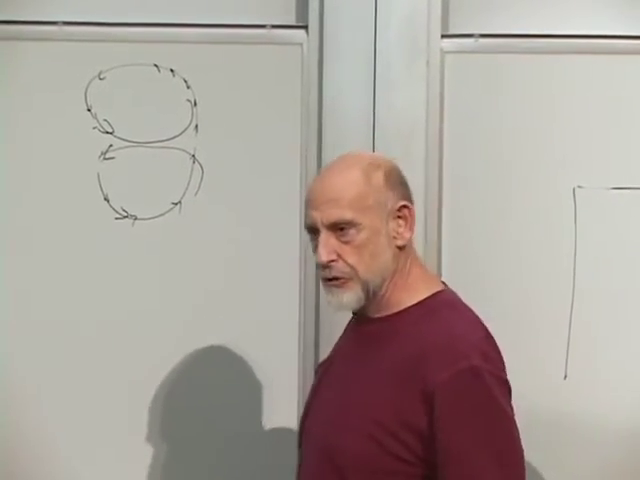
\includegraphics[width=0.72\textwidth]{lecture_10_figure_01.png}
  \caption{黑板上标出了两根闭弦及其相对取向。取向在分裂与合并过程中必须连续。}
  \lectureframe{00:05:40}
  \label{fig:l10-oriented-closed-strings}
\end{figure}

\begin{classroomqa}
\audiencequestion{如果世界面坐标从\(\sigma=0\)跑到\(2\pi\)，弦是否已经绕紧致方向走了一圈？\lecturetimestamp{00:08:42}}
\lecturerresponse{没有。坐标\(\sigma\)标记的是弦上的点；它并不标记紧致空间中的位置。每根闭弦都有一个周期性的参数\(\sigma\)，无论它是否缠绕。橡皮筋的类比很有用：即使橡皮筋没有绕在任何东西上，也可以给橡皮筋周围的分子编号。缠绕是映射\(Y(\tau,\sigma)\)的性质，而不是单由参数\(\sigma\)决定的性质。}
\end{classroomqa}

\begin{classroomqa}
\audiencequestion{紧致尺度是否也必须在大坐标\(X\)的每一个取值处都相同？\lecturetimestamp{00:10:00}}
\lecturerresponse{在一般的动力学紧致化中并非如此。我们从固定的圆开始，因为它是最干净的背景。后来，分量\(G_{55}\)将成为一个标量场，其取值度量第五方向的局部尺度，因此该尺度可以在普通时空上变化。}
\end{classroomqa}

\section{即使弦重新连接，缠绕也是守恒的}

一根未缠绕的弦可以穿过紧致方向而不绕它。缠绕的弦则不同：当\(\sigma\)绕闭弦走一圈时，嵌入\(Y(\tau,\sigma)\)前进一个或多个紧致圆的周期。因为弦是有向的，这一前进带有符号。弦可以沿正方向缠绕，也可以沿负方向缠绕。

守恒定律在合并的图像中最为清楚。取一根缠绕数为\(+1\)的弦和另一根缠绕数为\(-1\)的弦。它们相容的片段可以重新连接。所得位形具有零净缠绕数，并且可以形变为一根未缠绕的弦。黑板所描绘的正是这种相反取向的重新连接。

\begin{figure}[H]
  \centering
  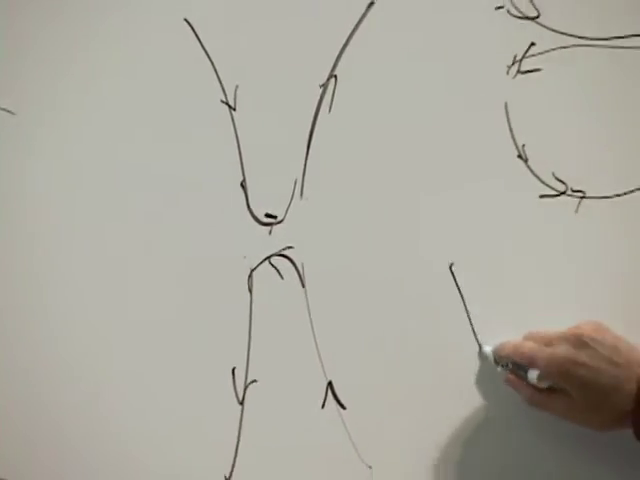
\includegraphics[width=0.72\textwidth]{lecture_10_figure_02.png}
  \medskip

  \begin{tikzpicture}[x=1cm,y=1cm,>=Latex]
    \draw[thick] (-4.0,0.3) circle (0.65);
    \draw[->,thick] (-4.55,0.58) arc (150:-145:0.65);
    \node at (-4.0,-0.65) {$w=+1$};
    \draw[thick] (-2.0,0.3) circle (0.65);
    \draw[<-,thick] (-2.55,0.58) arc (150:-145:0.65);
    \node at (-2.0,-0.65) {$w=-1$};
    \node at (-3.0,0.3) {$+$};
    \draw[->,thick] (-1.0,0.3) -- (0.3,0.3);
    \draw[thick] (1.4,0.3) ellipse (0.95 and 0.55);
    \node at (1.4,-0.65) {$w_{\rm total}=0$};
  \end{tikzpicture}
  \caption{相反绕数重新连接为零净绕数
  位形。下图是对黑板操作的清晰重构，而不是第二个动力学过程。}
  \lectureframe{00:13:20}
  \label{fig:l10-opposite-winding}
\end{figure}

现在用两根取向相同的弦重复该实验。它们可以连接，但不能退绕。结果携带任一根入射弦绕数的两倍。连接在一起的弦的数目改变了；总绕数没有改变。

\begin{figure}[H]
  \centering
  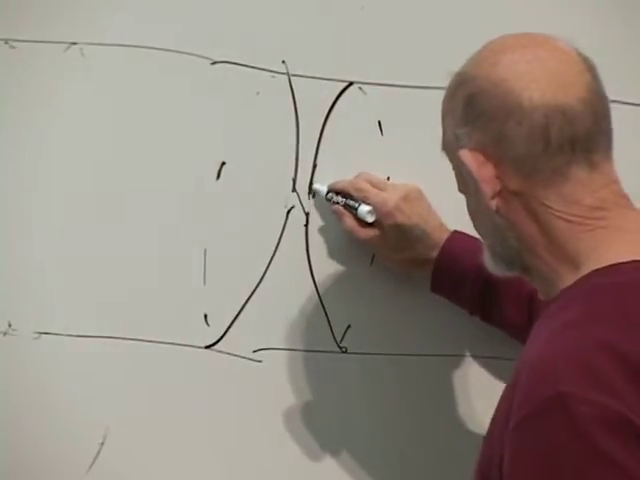
\includegraphics[width=0.72\textwidth]{lecture_10_figure_03.png}
  \medskip

  \begin{tikzpicture}[x=1cm,y=1cm,>=Latex]
    \draw[thick] (-4.0,0.3) circle (0.65);
    \draw[->,thick] (-4.55,0.58) arc (150:-145:0.65);
    \node at (-4.0,-0.65) {$w=+1$};
    \draw[thick] (-2.0,0.3) circle (0.65);
    \draw[->,thick] (-2.55,0.58) arc (150:-145:0.65);
    \node at (-2.0,-0.65) {$w=+1$};
    \node at (-3.0,0.3) {$+$};
    \draw[->,thick] (-1.0,0.3) -- (0.3,0.3);
    \draw[thick] (1.45,0.3) circle (0.78);
    \draw[thick] (1.45,0.3) circle (0.52);
    \draw[->,thick] (0.81,0.74) arc (145:-145:0.78);
    \node at (1.45,-0.78) {$w=+2$};
  \end{tikzpicture}
  \caption{同号绕数可以重新连接成一根双重缠绕的弦。
  连通性改变，而总绕数保持为二。}
  \lectureframe{00:16:40}
  \label{fig:l10-same-winding}
\end{figure}

这一区别在每一个允许的过程中都保持不变。总绕数一百可以由一根缠绕一百次的弦携带，由两根各缠绕五十次的弦携带，或由一百根单次缠绕的弦携带。弦可以在这些描述之间分裂和连接，但有符号之和保持为一百。我们将其记为\(w\in\mathbb Z\)。

\section{动量模式与绕数模式}

守恒本身还不是对偶性。接下来我们比较能量。一个绕紧致圆运动的态具有量子化动量
\begin{equation}
  p_Y=\frac{n}{R},
  \qquad n\in\mathbb Z.
  \label{eq:l10-compact-momentum}
\end{equation}
对于一个其他质量贡献可以忽略的态，紧致运动贡献\(E_{\rm mom}=|n|/R\)。正的和负的\(n\)表示相反的运动方向，而能量为正。

\begin{figure}[H]
  \centering
  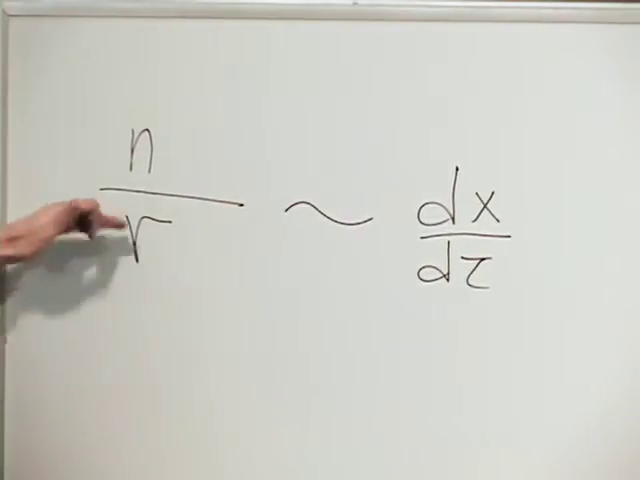
\includegraphics[width=0.72\textwidth]{lecture_10_figure_04.png}
  \caption{黑板上的紧致动量量子数。讲义将动量示意性地写为紧致速度的积分。}
  \lectureframe{00:21:30}
  \label{fig:l10-compact-momentum-board}
\end{figure}

一根缠绕\(|w|\)次的弦具有长度\(2\pi |w|R\)。以基本弦张力
\begin{equation}
  T_{\rm F}=\frac{1}{2\pi\alpha'},
\end{equation}
其绕数能量为
\begin{equation}
  E_{\rm wind}=T_{\rm F}(2\pi |w|R)
  =\frac{|w|R}{\alpha'}.
  \label{eq:l10-winding-energy}
\end{equation}
在讲义单位\(\alpha'=1\)下，这简单地就是\(E_{\rm wind}=|w|R\)。

当半径变化时，两座能级塔的行为相反。对于\(R\gg
\sqrt{\alpha'}\)，动量能级间距小，而绕数能级间距大。对于\(R\ll\sqrt{\alpha'}\)，动量能级间距大，而绕数能级间距小。

\begin{figure}[H]
  \centering
  \begin{minipage}[t]{0.48\textwidth}
    \centering
    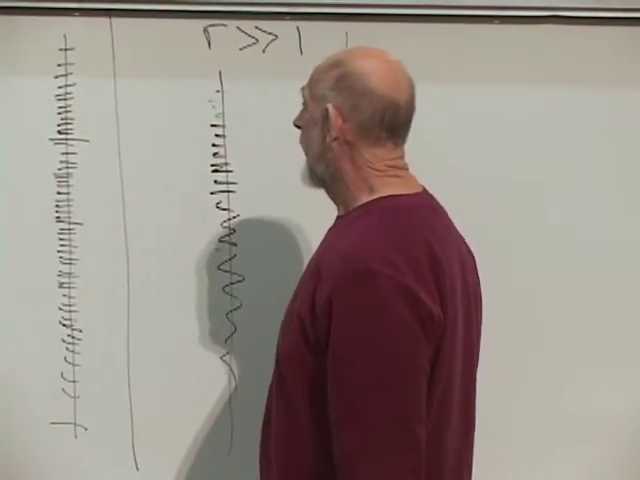
\includegraphics[width=\linewidth]{lecture_10_figure_05.png}
    \par\smallskip
    \textit{大紧致半径。}
  \end{minipage}\hfill
  \begin{minipage}[t]{0.48\textwidth}
    \centering
    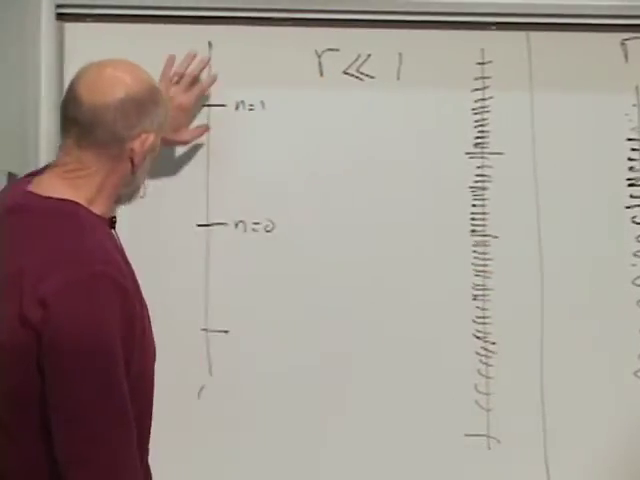
\includegraphics[width=\linewidth]{lecture_10_figure_06.png}
    \par\smallskip
    \textit{小紧致半径。}
  \end{minipage}
  \caption{黑板上的两个谱比较。当半径被反转时，稀疏和稠密的能级塔交换角色。}
  \lectureframe{00:25:30--00:26:00}
  \label{fig:l10-dual-spectra-board}
\end{figure}

清晰的示意图为
\begin{figure}[H]
  \centering
  \begin{adjustbox}{max width=\linewidth}
  \begin{tikzpicture}[x=1cm,y=0.74cm,>=Latex]
    \node[font=\bfseries] at (-3.6,6.2) {$R\gg\sqrt{\alpha'}$};
    \draw[->] (-5.1,0) -- (-5.1,5.5) node[above] {$E$};
    \foreach \y in {0.4,1.0,1.6,2.2,2.8,3.4,4.0,4.6}
      \draw (-5.35,\y)--(-4.85,\y);
    \node[align=center] at (-4.25,5.15) {momentum\\dense};
    \draw[->] (-2.2,0) -- (-2.2,5.5) node[above] {$E$};
    \foreach \y in {0.4,2.4,4.4}
      \draw (-2.45,\y)--(-1.95,\y);
    \node[align=center] at (-1.35,5.15) {winding\\sparse};

    \node[font=\bfseries] at (3.6,6.2) {$R\ll\sqrt{\alpha'}$};
    \draw[->] (2.2,0) -- (2.2,5.5) node[above] {$E$};
    \foreach \y in {0.4,2.4,4.4}
      \draw (1.95,\y)--(2.45,\y);
    \node[align=center] at (3.05,5.15) {momentum\\sparse};
    \draw[->] (5.1,0) -- (5.1,5.5) node[above] {$E$};
    \foreach \y in {0.4,1.0,1.6,2.2,2.8,3.4,4.0,4.6}
      \draw (4.85,\y)--(5.35,\y);
    \node[align=center] at (5.95,5.15) {winding\\dense};
  \end{tikzpicture}
  \end{adjustbox}
  \caption{能级间距论证的重构。当动量和绕数连同\(R\leftrightarrow\alpha'/R\)一起交换时，完整的弦谱不变。}
  \label{fig:l10-dual-spectra-redraw}
\end{figure}

假设一位观察者拿到这些谱中的一个，却没有被告知它是如何产生的。间距小的能级塔是大圆上的动量，还是小圆上的绕数？仅凭谱无法说明。弦理论给出更强的陈述：散射振幅也无法说明。这两种描述在
\begin{equation}
  n\longleftrightarrow w,
  \qquad
  R\longleftrightarrow \widetilde R=\frac{\alpha'}{R}.
  \label{eq:l10-radius-duality}
\end{equation}
下完全等价。不动点是
\begin{equation}
  R=\sqrt{\alpha'},
  \label{eq:l10-self-dual-radius}
\end{equation}
或在讲义单位下为\(R=1\)。在该半径处，额外的态可以变为无质量，并且规范对称性得到增强。

\begin{classroomqa}
\audiencequestion{绕数仅仅是为了重写谱而采用的数学便利吗？\lecturetimestamp{00:27:33}}
\lecturerresponse{不是。绕数标记闭弦希尔伯特空间的真实扇区，而这些扇区参与相互作用。``对偶''一词意味着动量描述和绕数描述是同一物理的不同坐标，而不是说一个扇区是另一个扇区的可选助记。}
\end{classroomqa}

\begin{classroomqa}
\audiencequestion{是否存在一个被映射到自身的半径？
\lecturetimestamp{00:27:58}}
\lecturerresponse{存在。自对偶值为
\(R=\sqrt{\alpha'}\)，在黑板所用单位下为\(R=1\)。两座能级塔在那里相遇，并且谱具有增强的对称性。}
\end{classroomqa}

\section{对偶性的世界面形式}

谱论证具有启发性，但世界面使这种交换更加精确。在共形规范中，与\(Y\)共轭的动量正比于\(\partial_\tau Y\)。因此总紧致动量具有形式
\begin{equation}
  P_Y=\frac{1}{2\pi\alpha'}
      \int_0^{2\pi}d\sigma\,\partial_\tau Y.
  \label{eq:l10-worldsheet-momentum}
\end{equation}
绕数为
\begin{equation}
  w=\frac{1}{2\pi R}
      \int_0^{2\pi}d\sigma\,\partial_\sigma Y
   =\frac{Y(2\pi)-Y(0)}{2\pi R}.
  \label{eq:l10-worldsheet-winding}
\end{equation}

\begin{classroomqa}
\audiencequestion{为什么导数的积分在闭合弦周围不会消失？\lecturetimestamp{00:32:33}}
\lecturerresponse{因为\(Y\)是一个周期性的靶空间坐标，而不是\(\sigma\)圆上的单值实函数。世界面点\(\sigma=2\pi\)与\(\sigma=0\)相同，但嵌入到覆盖线上的提升会改变\(2\pi wR\)。\(\partial_\sigma Y\)的积分衡量的正是这一移动。}
\end{classroomqa}

\begin{figure}[H]
  \centering
  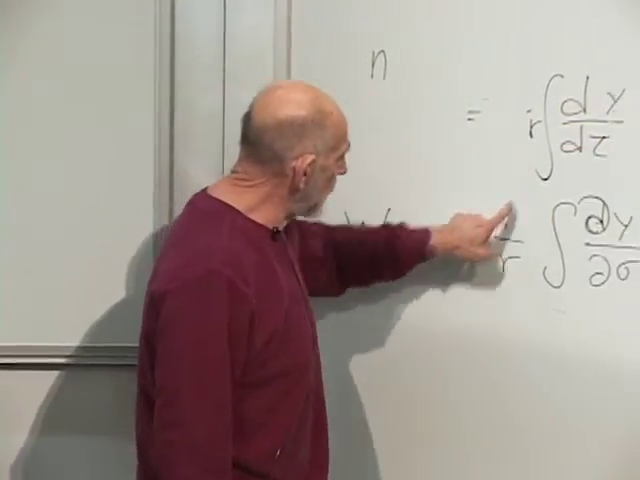
\includegraphics[width=0.76\textwidth]{lecture_10_figure_07.png}
  \caption{在板上完成两条线之后的动量与缠绕积分。常见的\(2\pi\)和\(\alpha'\)因子在讲座归一化中被省略。}
  \lectureframe{00:33:25}
  \label{fig:l10-momentum-winding-integrals}
\end{figure}

对于绕卷一次的弦，
\begin{equation}
  Y(\tau,\sigma+2\pi)=Y(\tau,\sigma)+2\pi R.
\end{equation}
对于缠绕数\(w\)，右侧的移动为\(2\pi wR\)。方程\eqref{eq:l10-worldsheet-winding}于是精确地计入了缠绕数。这就是板书简写\(w\sim R^{-1}\int
d\sigma\,\partial_\sigma Y\)的精确版本。

因此，T对偶的世界面表述为
\begin{equation}
  \partial_\tau Y\longleftrightarrow
  \partial_\sigma \widetilde Y,
  \qquad
  \partial_\sigma Y\longleftrightarrow
  \partial_\tau \widetilde Y,
  \label{eq:l10-derivative-duality}
\end{equation}
其中\(Y\)中的动量变为对偶坐标\(\widetilde Y\)中的缠绕，反之亦然。

\begin{classroomqa}
\audiencequestion{这是否意味着世界面坐标\(\tau\)和\(\sigma\)本身是相关的或互换的？\lecturetimestamp{00:34:39}}
\lecturerresponse{不。T对偶映射解，并交换紧致靶坐标的特定导数。它并不将世界面时间坐标与世界面空间坐标等同起来。}
\end{classroomqa}

\section{为什么缠绕态无法避免}

人们可能会问，当存在未缠绕态时，弦为什么还会处于缠绕态。弦并不按偏好选择自己的状态。碰撞中提供的能量会将它拉伸。一个能量足够高、高度畸变的弦可以重新连接成两根具有相反缠绕的弦。它们的总缠绕仍然为零，但在分裂之后，这两根弦可能分开。这对弦中的一个可以被送到很远的地方，使观察者面对一根看似孤立的缠绕弦。

\begin{figure}[H]
  \centering
  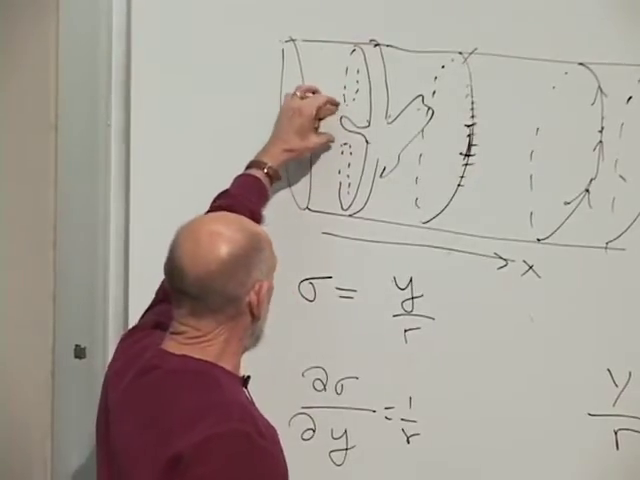
\includegraphics[width=0.76\textwidth]{lecture_10_figure_08.png}
  \caption{一个高度拉伸的零净缠绕构型，重新连接后相反缠绕的弦可以从中分离。}
  \lectureframe{00:36:15}
  \label{fig:l10-winding-pair-production}
\end{figure}

能量阈值由缠绕能设定。在一个大圆上，需要很大的碰撞能量才能将足够多的弦沿紧致方向拉伸。然而，在阈值以上，缠绕--反缠绕对产生不能被禁止。类比是光子碰撞产生电子--正电子对。总电荷仍然为零，但带电粒子确实存在并且可以被分开。缠绕守恒以同样的方式起作用。

这个类比不只是口头上的。紧致动量和缠绕表现为两个不同的荷量子数。在相应的约化描述中，同号相斥，异号相吸。因此，我们应当寻找传递这些力的两个矢量场。

\section{来自五维引力的动量荷}

从五维引力开始。令大写指标\(M,N\)遍历四个普通时空方向和紧致的第五方向。度规分解为
\begin{equation}
  G_{MN}\quad\longrightarrow\quad
  \bigl\{G_{\mu\nu},\,G_{\mu5},\,G_{55}\bigr\}.
  \label{eq:l10-metric-decomposition}
\end{equation}
对称分量\(G_{5\mu}\)除了\(G_{\mu5}\)之外不包含新信息。

\begin{figure}[H]
  \centering
  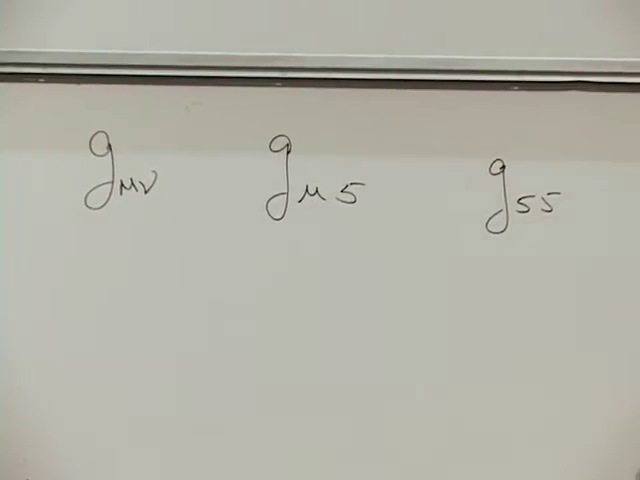
\includegraphics[width=0.74\textwidth]{lecture_10_figure_09.png}
  \caption{五维度规分量的独立分组：\(G_{\mu\nu}\)、\(G_{\mu5}\)和\(G_{55}\)。}
  \lectureframe{00:44:05}
  \label{fig:l10-metric-components}
\end{figure}

从四维观点看，
\begin{align}
  G_{\mu\nu} &\quad\hbox{is a spacetime metric},\\
  G_{\mu5} &\equiv A_\mu\quad\hbox{is a vector field},\\
  G_{55} &\equiv e^{2\varphi}\quad\hbox{is a scalar modulus}.
  \label{eq:l10-four-dimensional-fields}
\end{align}
标量\(\varphi\)衡量紧致方向的尺度。它可以在普通时空上平滑变化，因此\(\varphi\)的波就是第五维半径的波。

\begin{figure}[H]
  \centering
  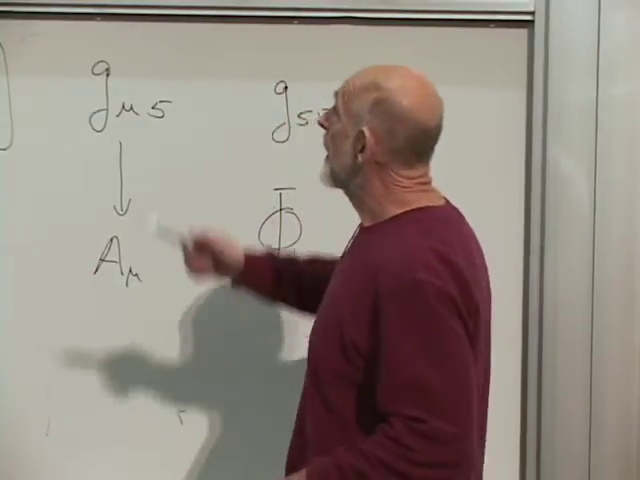
\includegraphics[width=0.74\textwidth]{lecture_10_figure_10.png}
  \caption{板书将\(G_{\mu5}\)等同于矢量\(A_\mu\)，将\(G_{55}\)等同于标量\(\Phi\)。}
  \lectureframe{00:47:40}
  \label{fig:l10-vector-and-radius-modulus}
\end{figure}

混合引力分量的源是混合动量流。特别地，沿第五方向的动量是\(G_{\mu5}\)的源。因此，四维观察者将整数\(n\)解释为耦合到\(A_\mu\)的电荷。这就是Kaluza--Klein机制：在高维几何中是动量的东西，在低维场论中变成电荷。

\editorialnote{讲座将来自\(G_{55}\)的标量粗略地称为``dilaton''。在这种约化中，它具体是半径模量。控制弦耦合的十维弦膨胀子是另一个场，尽管在改变标架和对偶下，低维标量组合可以混合。}

\begin{classroomqa}
\audiencequestion{标量\(\varphi\)是否正比于动量整数\(n\)？\lecturetimestamp{00:48:43}}
\lecturerresponse{不。整数\(n\)标记一个量子化态，并充当电荷。标量\(\varphi(x)\)是一个连续场，它决定局部的紧致化尺度。它可以随位置变化；它本身不是整数。}
\end{classroomqa}

\section{第二矢量场与缠绕荷}

缠绕也是类电荷的，但它不能以同样的方式耦合到同一个矢量。要看到第二个矢量，回到最初的闭弦激发。闭弦具有左行和右行振子模式。物理态满足能级匹配：左行和右行的总激发能级必须一致。

在玻色理论中，未激发态是快子。单个左行或右行振子会破坏能级匹配。因此第一个允许的无质量态包含每种振子各一个，
\begin{equation}
  \alpha_{-1}^{I}\widetilde\alpha_{-1}^{J}\ket{0;k}.
  \label{eq:l10-first-massless-state}
\end{equation}
指标\(I,J\)遍历横向空间方向，包括紧致方向。如果一个指标是普通的，另一个是\(5\)，则有两个类矢量振子态，
\begin{equation}
  \alpha_{-1}^{\mu}\widetilde\alpha_{-1}^{5}\ket{0;k},
  \qquad
  \alpha_{-1}^{5}\widetilde\alpha_{-1}^{\mu}\ket{0;k}.
  \label{eq:l10-two-vector-states}
\end{equation}

\begin{figure}[H]
  \centering
  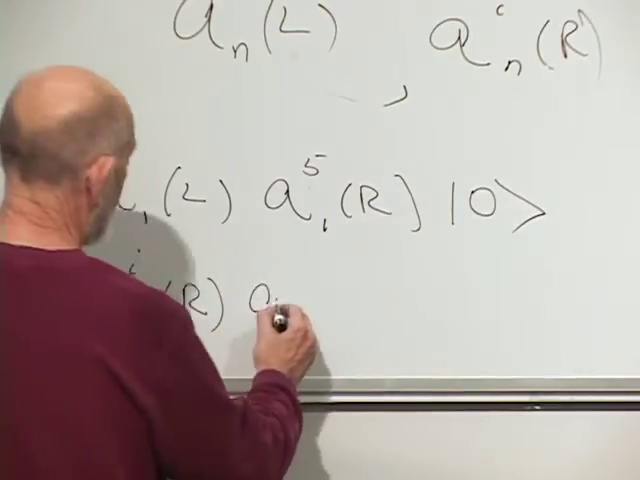
\includegraphics[width=0.76\textwidth]{lecture_10_figure_11.png}
  \caption{当其中一个极化沿紧致方向时，两种左--右振子排序成为四维矢量态。}
  \lectureframe{00:58:20}
  \label{fig:l10-two-vector-states-board}
\end{figure}

它们的对称和反对称组合属于不同的时空场：
\begin{align}
  \alpha_{-1}^{(\mu}\widetilde\alpha_{-1}^{5)}\ket{0;k}
    &\longleftrightarrow G_{\mu5},\\
  \alpha_{-1}^{[\mu}\widetilde\alpha_{-1}^{5]}\ket{0;k}
    &\longleftrightarrow B_{\mu5}.
  \label{eq:l10-g-and-b-vectors}
\end{align}
第一个是由紧致动量作为源的Kaluza--Klein矢量。第二个来自反对称的Kalb--Ramond场，并由弦缠绕作为源。因此，约化理论包含两个类光子场，每个电荷扇区各一个。

如果两个振子指标都沿紧致方向，则该态是与紧致化模量相关的标量。如果两者都在普通横向方向上，则对称无迹部分为引力子，反对称部分为\(B_{\mu\nu}\)，而迹则贡献到一个标量扇区。

\begin{classroomqa}
\audiencequestion{这些态中哪一个是单态，哪一个是三重态？\lecturetimestamp{01:00:21}}
\lecturerresponse{这种分类在这里不是有用的分类。两个混合态都作为四维矢量变换。它们的和与差将对称的度规极化与反对称的\(B\)场极化分开。具有两个紧致指标的态反而是四维标量。}
\end{classroomqa}

休息前得到的完整字典是
\begin{equation}
  \boxed{
  \begin{gathered}
    n\leftrightarrow w,
    \qquad
    R\leftrightarrow\dfrac{\alpha'}{R},\\
    \partial_\tau Y\leftrightarrow\partial_\sigma\widetilde Y,
    \qquad
    G_{\mu5}\leftrightarrow B_{\mu5}.
  \end{gathered}}
  \label{eq:l10-complete-t-duality-map}
\end{equation}

\begin{figure}[H]
  \centering
  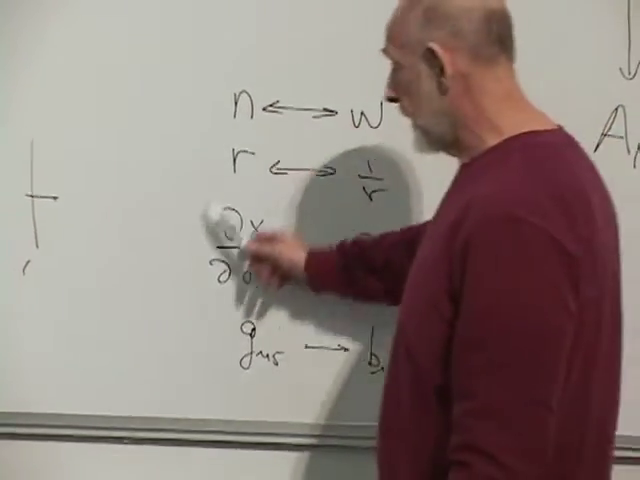
\includegraphics[width=0.72\textwidth]{lecture_10_figure_12.png}
  \caption{黑板上关于T对偶映射的总结：动量与缠绕、半径与倒数半径、世界面导数以及两个矢量场都被交换。讲演者部分遮挡了最后一行，因此该行在方程
  \eqref{eq:l10-complete-t-duality-map}中明确给出。}
  \lectureframe{01:02:20}
  \label{fig:l10-t-duality-map-board}
\end{figure}

不应将这一构造与如下主张混淆：刚刚列出的每个场都已经在观测到的粒子谱中被识别出来。在这一点上，它是紧致化弦理论的数学结果。有许多提议将这类结构与现象学联系起来，但这不是本讲所要解决的问题。

\section{开弦改变了问题}

休息之后，我们再次从开弦开始。闭弦可以具有稳定的缠绕，因为它没有端点可供缠绕滑脱。开弦有端点，因此没有类似的拓扑保护缠绕数。然而，T对偶是理论的精确对称性。这个对称性对开弦做了什么？

对于自由运动的端点，弦作用量的变分给出Neumann边界条件。在简单的\((X,Y)\)几何中，
\begin{equation}
  \left.\partial_\sigma X\right|_{\partial\Sigma}=0,
  \qquad
  \left.\partial_\sigma Y\right|_{\partial\Sigma}=0.
  \label{eq:l10-neumann-boundary}
\end{equation}
力学图像很直接。把弦看作由越来越小的质量元组成的链。对最后一个质量元施加非零的切向力，会使其加速度在其质量趋于零时发散。因此，自由端点会自行调整，直到端点净张力消失。人们也可以改为固定端点并提供所需的力，但那样端点就不再自由了。

\begin{figure}[H]
  \centering
  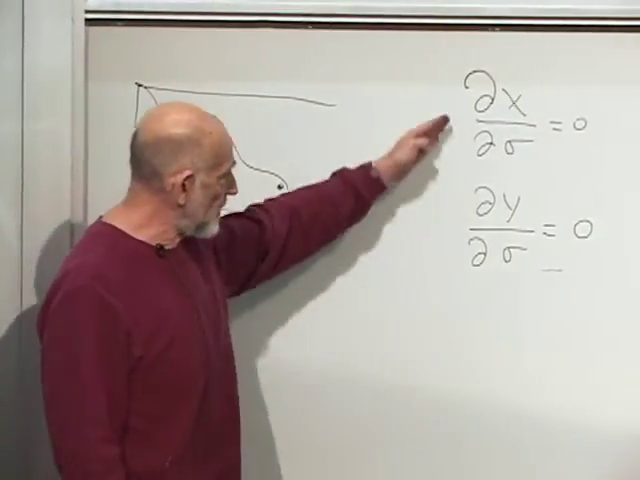
\includegraphics[width=0.76\textwidth]{lecture_10_figure_13.png}
  \caption{开弦及其完整的Neumann端点条件，\(\partial_\sigma X=\partial_\sigma Y=0\)。}
  \lectureframe{01:09:20}
  \label{fig:l10-neumann-board}
\end{figure}

现在只对紧致坐标\(Y\)做对偶化。非紧致坐标\(X\)保持不变。方程\eqref{eq:l10-derivative-duality}将第二个Neumann条件变为
\begin{equation}
  \left.\partial_\tau\widetilde Y\right|_{\partial\Sigma}=0.
  \label{eq:l10-dirichlet-time-derivative}
\end{equation}
因此，端点在対偶紧致方向上具有不依赖于时间的位置，
\begin{equation}
  \left.\widetilde Y\right|_{\partial\Sigma}=Y_0.
  \label{eq:l10-dirichlet-boundary}
\end{equation}
这就是Dirichlet边界条件。

\begin{figure}[H]
  \centering
  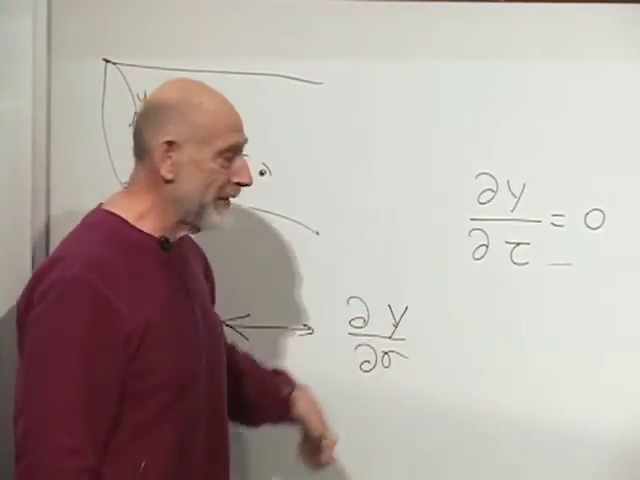
\includegraphics[width=0.76\textwidth]{lecture_10_figure_14.png}
  \medskip

  \begin{adjustbox}{max width=\linewidth}
  \begin{tikzpicture}[x=1cm,y=1cm,>=Latex]
    \node[align=center] at (-3.5,0.8)
      {Neumann\\\(\left.\partial_\sigma Y\right|_{\partial\Sigma}=0\)};
    \draw[->,thick] (-1.7,0.8) -- (1.3,0.8)
      node[midway,above] {$T_Y$};
    \node[align=center] at (3.4,0.8)
      {Dirichlet\\\(\left.\partial_\tau\widetilde Y\right|_{\partial\Sigma}=0\)};
    \node[align=center] at (3.4,-0.5)
      {\(\widetilde Y(\tau)=Y_0\) at each endpoint};
  \end{tikzpicture}
  \end{adjustbox}
  \caption{黑板上完成的对偶端点条件及其清晰的逻辑重构。T对偶将紧致方向上的自由度变为对偶方向上的固定端点位置。}
  \lectureframe{01:12:35}
  \label{fig:l10-neumann-to-dirichlet}
\end{figure}

\begin{classroomqa}
\audiencequestion{为什么対偶条件意味着端点是固定的？\lecturetimestamp{01:12:39}}
\lecturerresponse{因为\(\partial_\tau\widetilde Y=0\)在対偶化方向上的速度为零。无论端点在\(\widetilde Y\)中从哪里开始，它都停留在那里。其平行于未対偶化方向的坐标仍然是自由的。}
\end{classroomqa}

\section{持有端点的物体是D膜}

如果端点被固定，那么必须有某种东西能够把它保持在那里。因此，精确的T对偶要求存在一种新的物体，开弦可以终止于其上。这种物体就是D膜。字母\(D\)代表Dirichlet，而不是该物体的维度。在讲座的历史旁注中，这些物体或许会以Joseph Polchinski命名，因为他的分析使它们的动力学作用变得无可置疑，但已经确立的术语``p膜''使得Dirichlet成为自然的名称。

一个\(p\)膜具有\(p\)个空间维度。弦是一膜，膜是二膜，而延展的三维物体是三膜。一个D\(p\)膜是一个\(p\)膜，基本弦的端点在其横向方向上服从Dirichlet条件，而在与膜相切的方向上服从Neumann条件。

对偶论证中没有任何东西挑出\(Y_0\)的某一个值，因此D膜不可能是钉在宇宙中某个优先点上的刚性固定物。它必须是可移动的。相对论也禁止绝对刚性的延展物体，因此D膜可以涨落和弯曲。黑板上画出的简单平坦膜是它的平衡构型，而不是对其动力学的限制。

\begin{classroomqa}
\audiencequestion{开弦的两个端点是否必须具有相同的対偶坐标固定值？\lecturetimestamp{01:14:55}}
\lecturerresponse{一般来说不是。两个端点可以位于同一个D膜上，在这种情况下它们共享该膜的横向位置。它们也可以位于两个处于不同横向位置的不同D膜上，于是弦在它们之间拉伸。膜本身可以涨落和弯曲，因此端点轨迹不必保持为完全平坦的平面。}
\end{classroomqa}

\section{计算D膜的维度}

十维超弦理论有九个空间维度。假设T对偶在一个空间方向上施加Dirichlet条件。端点在其余八个方向上仍然是自由的，因此其允许的轨迹是一个八维D8膜。每增加一个独立的Dirichlet条件，就移除端点运动的一个方向。如果\(k\)个空间坐标被固定，那么
\begin{equation}
  p=9-k.
  \label{eq:l10-dp-counting}
\end{equation}

桌面给出了同一计数的三维版本。固定竖直坐标，指尖可以在二维桌面上移动。固定第二个坐标，它就只能沿一条线移动。固定全部三个坐标，它就被限制在一个点上。

\begin{figure}[H]
  \centering
  \begin{adjustbox}{max width=\linewidth}
  \begin{tikzpicture}[x=1.05cm,y=1cm,>=Latex]
    \draw[fill=blue!8] (-5.5,-0.7) -- (-2.5,-0.7) -- (-1.7,0.2)
      -- (-4.7,0.2) -- cycle;
    \node at (-3.6,-1.15) {one constraint: sheet};
    \draw[very thick,blue!60!black] (-0.9,-0.25) -- (1.3,-0.25);
    \node at (0.2,-1.15) {two constraints: line};
    \fill[blue!70!black] (4.1,-0.25) circle (0.09);
    \node at (4.1,-1.15) {three constraints: point};
    \draw[->] (-1.45,0.95) -- (-0.75,0.95);
    \draw[->] (2.25,0.95) -- (2.95,0.95);
    \node at (0.35,1.35) {each Dirichlet condition lowers \(p\) by one};
  \end{tikzpicture}
  \end{adjustbox}
  \caption{在桌面处使用的维度计数论证。D\(p\)膜是端点在其中仍可自由移动的轨迹。}
  \label{fig:l10-dp-counting-redraw}
\end{figure}

反复进行对偶化会生成D8膜、D7膜、D6膜等等，直到D0膜，它在空间中是点状的。如果没有空间方向被固定，一个D9膜填满全部九个空间维度，普通开弦可以在各处自由移动。讲座简要提到了D\((-1)\)膜；它们在欧几里得时空中是局域化的，其行为像瞬子，而不是像在时间中传播的普通粒子。

\editorialnote{维度阶梯是关于类型II理论合在一起的一个陈述。稳定的BPS D\(p\)膜在类型IIA中具有偶数\(p\)，在类型IIB中具有奇数\(p\)。沿一个圆进行T对偶会使\(p\)改变一，同时将类型IIA与类型IIB互换。}

\begin{classroomqa}
\audiencequestion{如果只有六个维度是紧致的，那么计数是否应当从六而不是从九开始减？\lecturetimestamp{01:20:49}}
\lecturerresponse{这一初等推导对紧致方向施行T对偶，但当一个圆变得任意小时，其对偶圆会变得任意大。在该极限下，它实际上是无限大的。因此，所得出的膜可以沿着在可及尺度上看似无限大的方向延展，也可以与之横截。维度\(p\)计数的是与膜相切的所有空间方向，而不仅仅是某一种推导中所用的紧致方向。}
\end{classroomqa}

D0膜是一种新型粒子。一根开弦可以从一个D0膜延伸到另一个D0膜，也可以回到同一个D膜，或者伸向一个非常遥远的膜。若把弦按字面意义延伸到空间无限远处，它便具有无限长度，因而具有无限能量，所以物理上有用的版本是把它的另一个端点放在另一个物体上。

下一个情形，即D1膜，本身是弦状的，但它并不是我们一开始所讨论的基本弦。它可以弯曲并闭合成自身，而基本弦可以终止于其上。它的张力对弦耦合常数的标度关系不同：
\begin{equation}
  T_{\rm D1}=\frac{1}{2\pi\alpha' g_s},
  \qquad
  T_{\rm F1}=\frac{1}{2\pi\alpha'}.
  \label{eq:l10-dstring-tension}
\end{equation}
在弱耦合\(g_s\ll1\)下，D弦比基本弦重得多，这解释了为什么它最初表现为一个质量巨大的锚点。

\begin{figure}[H]
  \centering
  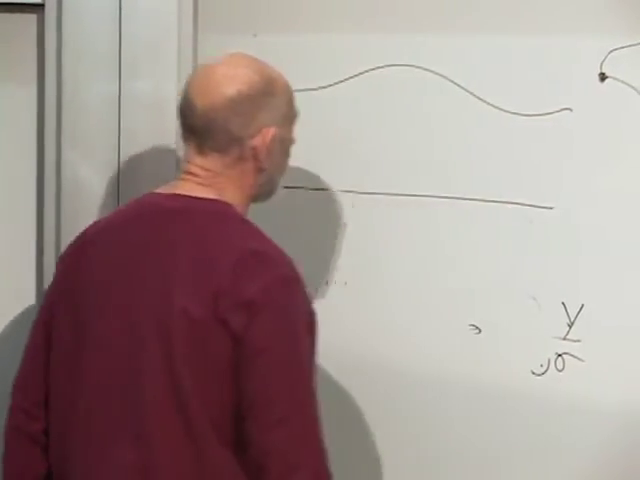
\includegraphics[width=0.76\textwidth]{lecture_10_figure_15.png}
  \caption{黑板上的D1膜：一个可弯曲的一维物体，不同于可以终止于其上的基本弦。}
  \lectureframe{01:24:20}
  \label{fig:l10-d1-brane}
\end{figure}

\begin{classroomqa}
\audiencequestion{T对偶是否既作用于弦，也作用于D膜？\lecturetimestamp{01:25:35}}
\lecturerresponse{是的。平行于D\(p\)膜的T对偶将其维度降低为D\((p-1)\)，而横截于它的T对偶将其维度升高为D\((p+1)\)。膜是对偶词典的一部分，而不是在对偶下保持不变的、外部的支撑物。}
\end{classroomqa}

\begin{classroomqa}
\audiencequestion{与膜相切的方向是否仍可以是紧致的？\lecturetimestamp{01:27:25}}
\lecturerresponse{是的。``相切''与``紧致''回答的是不同的问题。一个方向可以沿着膜，同时仍闭合成一个圆；它也可以是非紧致的。对端点而言，重要的是该方向上的边界条件是诺伊曼型还是狄利克雷型。}
\end{classroomqa}

D2膜是类似膜片的薄片。D3膜有三个空间维度。在真正高维的时空中，D3膜是一个三维子空间，而不是整个空间，尽管被限制在其上的观测者可能会把它体验为自己的整个空间世界。

\begin{figure}[H]
  \centering
  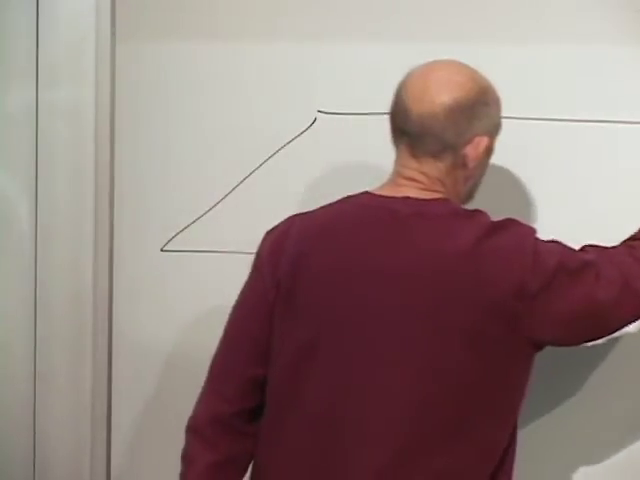
\includegraphics[width=0.76\textwidth]{lecture_10_figure_16.png}
  \caption{一个画成薄片的D2膜，弦的端点可以在其上移动。}
  \lectureframe{01:27:55}
  \label{fig:l10-d2-brane}
\end{figure}

这里给出的推导有意只是一个梗概。它本身并不能证明弦理论描述了自然。然而，在弦理论内部，一致性检验为数众多：对偶性、量子计算和数学结果都指向D膜是真正的动力学物体。

\section{开弦成为膜上的场}

取一个除此之外空无一物的D2膜，并把短开弦放在其上。每个端点都被限制在薄片内，因此整个低能激发沿着薄片运动。两根有向弦，若其相邻端点带有相容的箭头，便可以接合。接合后的弦之后可以再次分裂。若读作粒子历史，这些就是费曼图的顶点：两个粒子进入，一个中间激发传播，两个粒子出来。

\begin{figure}[H]
  \centering
  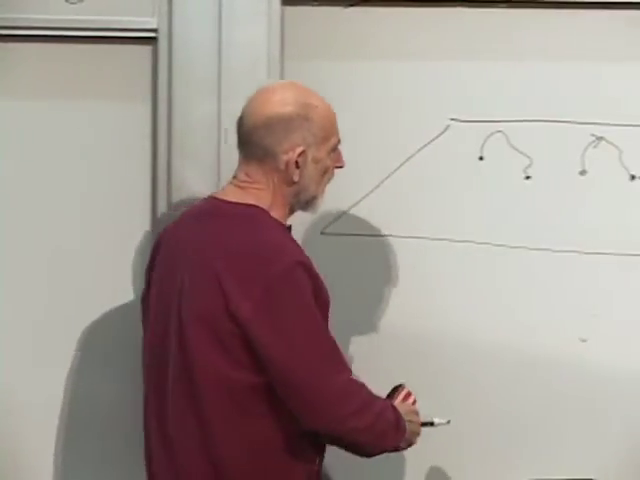
\includegraphics[width=0.76\textwidth]{lecture_10_figure_17.png}
  \caption{D2膜上的有向开弦通过相容的端点接合。在低能下，该过程被读作膜上的场论相互作用。}
  \lectureframe{01:29:55}
  \label{fig:l10-open-strings-on-brane}
\end{figure}

在远低于弦标度的能量下，内部振动谱塔不会被激发。剩下的无质量开弦态是膜世界体上的一个矢量场。对于单个膜，这是一个阿贝尔\(U(1)\)规范场，即电磁学在膜上的对应物。该场并不传播通过整个十维体空间；它的量子是开弦，其端点把它们保持在膜上。

\section{一叠膜产生非阿贝尔色}

现在把若干平行的膜放在彼此附近。对于三张膜，将它们标记为红、绿、蓝。一根有向弦具有一对有序的端点标签：它可以从红到绿、从绿到蓝、从红到红，等等。对于\(N\)张膜，无质量开弦态可以排列成一个\(N\times N\)矩阵
\begin{equation}
  A_\mu{}^{i}{}_{j},
  \qquad i,j=1,\ldots,N.
  \label{eq:l10-chan-paton-matrix}
\end{equation}
这些就是\(U(N)\)规范理论的Chan--Paton标签。

\begin{figure}[H]
  \centering
  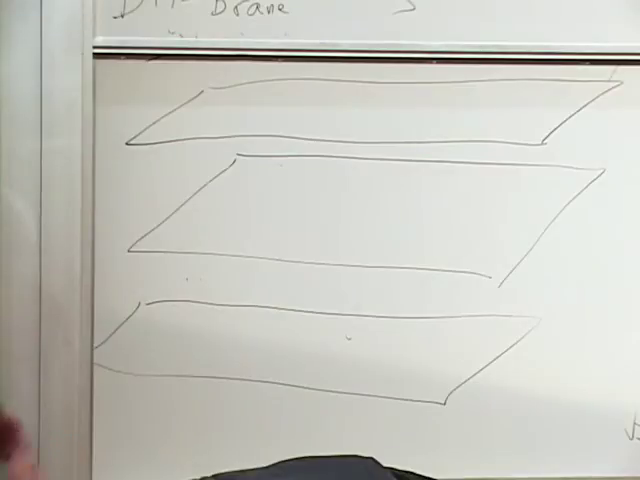
\includegraphics[width=0.76\textwidth]{lecture_10_figure_18.png}
  \medskip

  \begin{adjustbox}{max width=\linewidth}
  \begin{tikzpicture}[x=1cm,y=1cm,>=Latex]
    \draw[very thick,red!70!black] (-4.8,2.0)--(4.8,2.0);
    \draw[very thick,green!55!black] (-4.8,0.8)--(4.8,0.8);
    \draw[very thick,blue!70!black] (-4.8,-0.4)--(4.8,-0.4);
    \node[left] at (-4.8,2.0) {Red};
    \node[left] at (-4.8,0.8) {Green};
    \node[left] at (-4.8,-0.4) {Blue};
    \draw[->,thick] (-3.4,2.0) .. controls (-2.8,1.35) and (-2.3,1.15)
      .. (-1.7,0.8);
    \node at (-2.7,1.05) {$R\!G$};
    \draw[->,thick] (-0.6,0.8) .. controls (0.0,0.25) and (0.6,-0.05)
      .. (1.2,-0.4);
    \node at (0.1,0.0) {$G\!B$};
    \draw[->,thick] (2.1,2.0) .. controls (2.9,2.55) and (3.8,2.55)
      .. (4.3,2.0);
    \node at (3.2,2.65) {$R\!R$};
  \end{tikzpicture}
  \end{adjustbox}
  \caption{黑板上的三张平行膜，以及它们之间弦所携带的有序端点标签的清晰重构。}
  \lectureframe{01:33:15}
  \label{fig:l10-three-brane-stack}
\end{figure}

\begin{classroomqa}
\audiencequestion{一根弦真的能从红膜跑到绿膜，而不被其他图形挡住吗？\lecturetimestamp{01:35:07}}
\lecturerresponse{是的。这些膜嵌在更高维的空间中。二维的黑板图像只是一个投影，所以一根弦可以沿横向绕过另一条投影线。}
\end{classroomqa}

\begin{classroomqa}
\audiencequestion{一根红--绿弦必须与一根绿--蓝弦结合，才能变成红--蓝弦吗？\lecturetimestamp{01:35:39}}
\lecturerresponse{这就是基本的局部连接规则。相容的端点相遇，两段弦变成一根弦，其未连接的端点保留它们的红、蓝标签。更复杂的过程通过重复同一操作来构建。}
\end{classroomqa}

连接规则就是几何化的矩阵乘法。一根红--绿弦可以与一根绿--蓝弦连接，因为其中一根弦的绿端点与另一根弦的绿端点相容。结果是红--蓝弦：
\begin{equation}
  (R,G)\circ(G,B)\longrightarrow(R,B).
  \label{eq:l10-color-composition}
\end{equation}
重复的指标被连接并在内部消失。这与Yang--Mills相互作用顶点处出现的指标结构相同。

\begin{figure}[H]
  \centering
  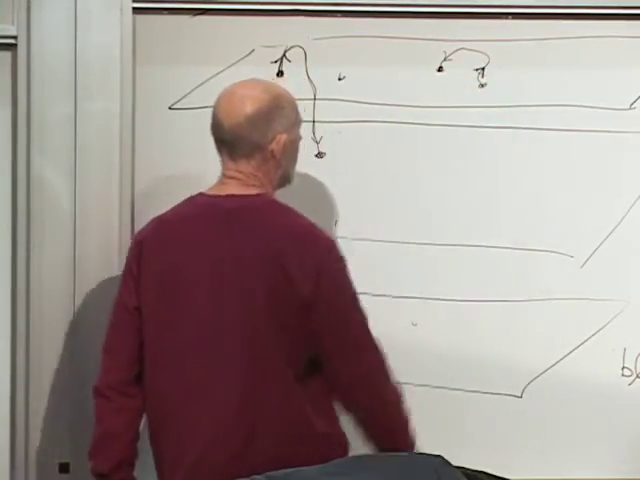
\includegraphics[width=0.76\textwidth]{lecture_10_figure_19.png}
  \caption{在膜堆上连接开弦。端点取向强制采用与非阿贝尔规范场相同的有序指标合成。}
  \lectureframe{01:36:30}
  \label{fig:l10-color-joining-board}
\end{figure}

对于三张重合的膜，完整的开弦规范群是\(U(3)\)，有九个矢量态。其代数分解为
\begin{equation}
  \mathfrak u(3)=\mathfrak{su}(3)\oplus\mathfrak u(1).
  \label{eq:l10-u3-decomposition}
\end{equation}
八个无迹组合具有QCD胶子的色结构，而对角质心\(U(1)\)是一个单独的阿贝尔场。

\editorialnote{讲座将九种色对组合之一描述为能够脱离并消失，从而留下八个胶子。精确的D膜陈述是：三张重合膜的堆给出\(U(3)\)，而不仅仅是\(SU(3)\)。要得到QCD八重态，需要分离、投影掉或以其他方式解耦对角\(U(1)\)。讲座的图像正确地启发了有序色指标，但它并不是对QCD的完整推导。}

类夸克物质只携带一个色指标。在膜图像中，它由一根弦表示，弦的一个端点位于色膜堆上，另一个端点位于另一张不同的、遥远的膜上。相对于色膜堆，只有一个端点作为色标签可见。反转取向就得到反粒子。一根类夸克弦和一根类反夸克弦若端点相容，就可以连接并离开色膜堆；两根取向相同的类夸克弦不能以这种方式湮灭。

由此得到的低能理论一般是超对称Yang--Mills理论，其附加物质由膜及其相交决定。它们与QCD足够接近，可以阐明非阿贝尔动力学，但它们并不自动就是标准模型。只有一张膜时，同样的构造约化为\(U(1)\)理论：短的膜--膜弦是类光子的，而到达第二个扇区的有向弦扮演正、负电荷的角色。

\section{D弦以磁单极子为终点}

现在故事中有两种类弦物体。原本的基本弦，即F弦，在D3膜上携带电流。D1膜，即D弦，在弱耦合下重得多。D弦也可以终止于D3膜上。它的端点在世界体规范场下不带电荷；它带磁荷。从D3膜上的观察者来看，该端点是一个磁单极子。

\begin{figure}[H]
  \centering
  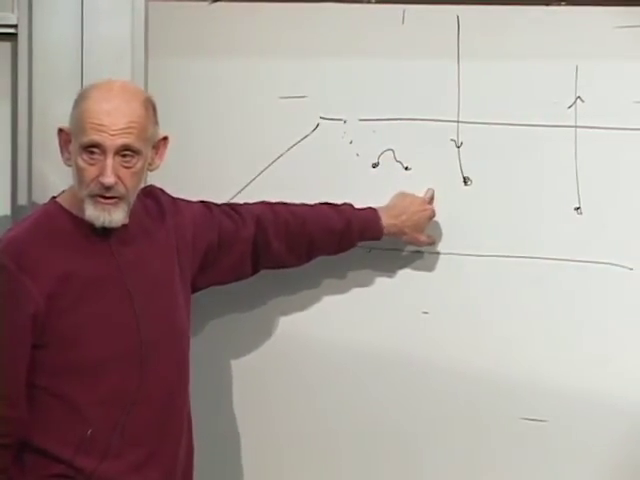
\includegraphics[width=0.76\textwidth]{lecture_10_figure_20.png}
  \medskip

  \begin{adjustbox}{max width=\linewidth}
  \begin{tikzpicture}[x=1cm,y=1cm,>=Latex]
    \draw[fill=blue!7] (-3.8,-0.5)--(2.6,-0.5)--(3.6,0.35)--(-2.8,0.35)--cycle;
    \node at (2.25,-0.95) {D3-brane};
    \draw[very thick,red!70!black] (0.0,3.0)--(0.0,0.0);
    \fill[black] (0.0,0.0) circle (0.08);
    \node[right] at (0.15,2.1) {D-string};
    \foreach \a in {25,65,115,155} {
      \draw[->,blue!65!black] (0.0,0.0)--({1.25*cos(\a)},{0.65*sin(\a)});
    }
    \node[align=center] at (4.8,1.7) {magnetic flux\\on the D3 worldvolume};
    \draw[->] (3.7,1.35)--(1.05,0.45);
  \end{tikzpicture}
  \end{adjustbox}
  \caption{黑板上的端点构造及其清晰解释。一根终止于D3膜上的D弦，对世界体规范理论而言表现为磁单极子。}
  \lectureframe{01:41:30}
  \label{fig:l10-dstring-monopole}
\end{figure}

质量等级结构也具有正确的定性形式。由于D弦张力带有因子\(1/g_s\)，在弱耦合下其端点比普通的电激发重得多。F弦与D弦端点之间的电/磁关系是IIB型弦理论更广泛对偶结构的一部分。

\begin{classroomqa}
\audiencequestion{D弦的端点是中性的吗？
\lecturetimestamp{01:42:19}}
\lecturerresponse{相对于基本弦端点所携带的电荷而言，它是中性的，但它并非不带电。它携带磁荷，因此是D3膜规范理论中的磁单极子。}
\end{classroomqa}

\section{该构造声称了什么，又没有声称什么}

从T对偶到膜的这条道路是历经数十年逐步拼合而成的，而非出自单一计算。一个最初为描述强子而提出的理论，变成了量子引力的候选理论。它的对偶性随后把D膜逼入谱中，而规范理论又作为终结于这些膜上的弦的低能动力学重新出现。在这个意义上，这门学科兜了一个完整的圈子。

D膜及相关的对偶构造已成为研究超对称规范理论、强耦合系统以及引力与场论之间联系的有力工具。它们还通过规范/引力对偶为流体和等离子体模型提供了启示。这一成功并不等同于直接推导出观测到的粒子谱。紧致化几何、膜位形、超对称破缺以及许多其他要素仍然有待选定。

\begin{classroomqa}
\audiencequestion{是什么决定了哪一个紧致维度被对偶化？
\lecturetimestamp{01:44:59}}
\lecturerresponse{从数学上说，只要所需对称性存在，就可以对任何紧致方向做对偶，并选择最方便的描述。从物理上说，在某一特定状态中实现的膜取向和紧致化数据，是由该状态的历史和动力学所选择的。}
\end{classroomqa}

\begin{classroomqa}
\audiencequestion{磁单极子构造由哪一种膜承载？
\lecturetimestamp{01:45:21}}
\lecturerresponse{规范理论所经历的世界是一张D3膜。D弦延伸到横向方向并终结于那张D3膜上；它的端点就是在该膜的三维空间中所见的磁单极子。}
\end{classroomqa}

\begin{classroomqa}
\audiencequestion{D弦也是有取向的吗？
\lecturetimestamp{01:45:55}}
\lecturerresponse{是的。反转D弦的取向会反转相应的荷。两种端点取向区分磁单极子与反磁单极子，正如取向对基本弦端点区分电荷一样。}
\end{classroomqa}

\begin{classroomqa}
\audiencequestion{这个简单的环面图像能解释手征粒子物理的左--右不对称性吗？
\lecturetimestamp{01:46:05}}
\lecturerresponse{仅凭它本身不能。平坦环面过于对称。手征谱需要更多结构，例如不对称的膜相交、orbifold投影，或在合适的Calabi--Yau几何上的紧致化。弦理论具有产生手征性的机制，但它们超出了这一初等T对偶构造的范围。}
\end{classroomqa}

我们追踪了一种对称性历经四种具体形式：谱的交换、世界面导数的交换、时空场的交换，最后是端点边界条件的交换。最后一种形式是决定性的。它把一种数学等价性转变为D膜的发现，并把开弦的动力学转变为其世界体积上的规范理论。到了这一步，用Susskind的话说，这场讲座已经用尽了它的时间、能量和动量。
\end{document}
